\documentclass[b5paper,]{book}
\usepackage{lmodern}
\usepackage{amssymb,amsmath}
\usepackage{ifxetex,ifluatex}
\usepackage{fixltx2e} % provides \textsubscript
\ifnum 0\ifxetex 1\fi\ifluatex 1\fi=0 % if pdftex
  \usepackage[T1]{fontenc}
  \usepackage[utf8]{inputenc}
  \usepackage{eurosym}
\else % if luatex or xelatex
  \ifxetex
    \usepackage{mathspec}
  \else
    \usepackage{fontspec}
  \fi
  \defaultfontfeatures{Ligatures=TeX,Scale=MatchLowercase}
  \newcommand{\euro}{€}
\fi
% use upquote if available, for straight quotes in verbatim environments
\IfFileExists{upquote.sty}{\usepackage{upquote}}{}
% use microtype if available
\IfFileExists{microtype.sty}{%
\usepackage{microtype}
\UseMicrotypeSet[protrusion]{basicmath} % disable protrusion for tt fonts
}{}
\usepackage[margin=1in]{geometry}
\usepackage{hyperref}
\hypersetup{unicode=true,
            pdfborder={0 0 0},
            breaklinks=true}
\urlstyle{same}  % don't use monospace font for urls
\usepackage{natbib}
\bibliographystyle{apalike}
\usepackage{longtable,booktabs}
\usepackage{graphicx,grffile}
\makeatletter
\def\maxwidth{\ifdim\Gin@nat@width>\linewidth\linewidth\else\Gin@nat@width\fi}
\def\maxheight{\ifdim\Gin@nat@height>\textheight\textheight\else\Gin@nat@height\fi}
\makeatother
% Scale images if necessary, so that they will not overflow the page
% margins by default, and it is still possible to overwrite the defaults
% using explicit options in \includegraphics[width, height, ...]{}
\setkeys{Gin}{width=\maxwidth,height=\maxheight,keepaspectratio}
\IfFileExists{parskip.sty}{%
\usepackage{parskip}
}{% else
\setlength{\parindent}{0pt}
\setlength{\parskip}{6pt plus 2pt minus 1pt}
}
\setlength{\emergencystretch}{3em}  % prevent overfull lines
\providecommand{\tightlist}{%
  \setlength{\itemsep}{0pt}\setlength{\parskip}{0pt}}
\setcounter{secnumdepth}{5}
% Redefines (sub)paragraphs to behave more like sections
\ifx\paragraph\undefined\else
\let\oldparagraph\paragraph
\renewcommand{\paragraph}[1]{\oldparagraph{#1}\mbox{}}
\fi
\ifx\subparagraph\undefined\else
\let\oldsubparagraph\subparagraph
\renewcommand{\subparagraph}[1]{\oldsubparagraph{#1}\mbox{}}
\fi

%%% Use protect on footnotes to avoid problems with footnotes in titles
\let\rmarkdownfootnote\footnote%
\def\footnote{\protect\rmarkdownfootnote}

%%% Change title format to be more compact
\usepackage{titling}

% Create subtitle command for use in maketitle
\newcommand{\subtitle}[1]{
  \posttitle{
    \begin{center}\large#1\end{center}
    }
}

\setlength{\droptitle}{-2em}

  \title{}
    \pretitle{\vspace{\droptitle}}
  \posttitle{}
    \author{}
    \preauthor{}\postauthor{}
    \date{}
    \predate{}\postdate{}
  
\usepackage{booktabs}
\usepackage{booktabs}
\usepackage{longtable}
\usepackage{array}
\usepackage{multirow}
\usepackage[table]{xcolor}
\usepackage{wrapfig}
\usepackage{float}
\usepackage{colortbl}
\usepackage{pdflscape}
\usepackage{tabu}
\usepackage{threeparttable}
\usepackage{threeparttablex}
\usepackage[normalem]{ulem}
\usepackage{makecell}

\usepackage{amsthm}
\newtheorem{theorem}{Theorem}[chapter]
\newtheorem{lemma}{Lemma}[chapter]
\theoremstyle{definition}
\newtheorem{definition}{Definition}[chapter]
\newtheorem{corollary}{Corollary}[chapter]
\newtheorem{proposition}{Proposition}[chapter]
\theoremstyle{definition}
\newtheorem{example}{Example}[chapter]
\theoremstyle{definition}
\newtheorem{exercise}{Exercise}[chapter]
\theoremstyle{remark}
\newtheorem*{remark}{Remark}
\newtheorem*{solution}{Solution}
\begin{document}

{
\setcounter{tocdepth}{1}
\tableofcontents
}
\part{Introduction}\label{part-introduction}

The information field human beings are living in has changed
dramatically over the last years, effecting economy, technology, culture
and society. And yet, its stronger mark has been over business systems
\citep{Arun2006Firm, jin2015significance, degryse2016digitalisation, john2014big, o2016weapons}:
companies have to master methods and tools to solve the information
overload issue in order to strive and stay competitive
\citep{levitin2014organized, feng2015competing}.

To understand what companies go through in terms of challenges, we have
to wear their shoes. Let's say that the amount of information (such as
tactile, visual and sounds, rumors and conversations, the content of
business papers) gathered in the location we live in starts to rise
quickly. To survive such an environment, we would need new and more
powerful senses; we would probably need outside systems to help us
processing information. Considering the mole of digital information
produced in the past 10 years, companies have found themselves in our
hypothetical scenario: their digital universe is chaotic and constantly
expanding. In fact, this very universe will grow from 2005 to 2020, from
130 exabytes to 40,000 exabytes (40 zettabytes)
\citep{gantz2012digital}, as shown in figure \ref{fig:biginfo}.

Moreover, new digital technologies have had an impact outside but most
importantly inside companies
\citep{lasi2014industry, brettel2014virtualization, russmann2015industry}.
Thanks to Industry 4.0, it is possible to create a low-budget digital
copy of the company; in other terms, it is economically sustainable to
extract information from any business process
\citep{davies2015industry}. Even though it seems a great advantage for
companies, it leads to an information overload as an internal issue
which should be handled as an external one.

Inside this rising pressure, the general goal of the present thesis is
to understand how this information can be turned in to technical
knowledge by technical experts (e.g.~engineers, researchers, managers,
marketeers). In order to do that, this work investigates:

\begin{itemize}
\tightlist
\item
  where valuable business information is hidden in certain documents
\item
  which technical knowledge can be extracted from different sources of
  information
\item
  what methods and software are available in order to reach this goal
\item
  how these tools can be redesigned (if necessary) for being effective
  in non-standard contexts
\end{itemize}

\begin{figure}

{\centering 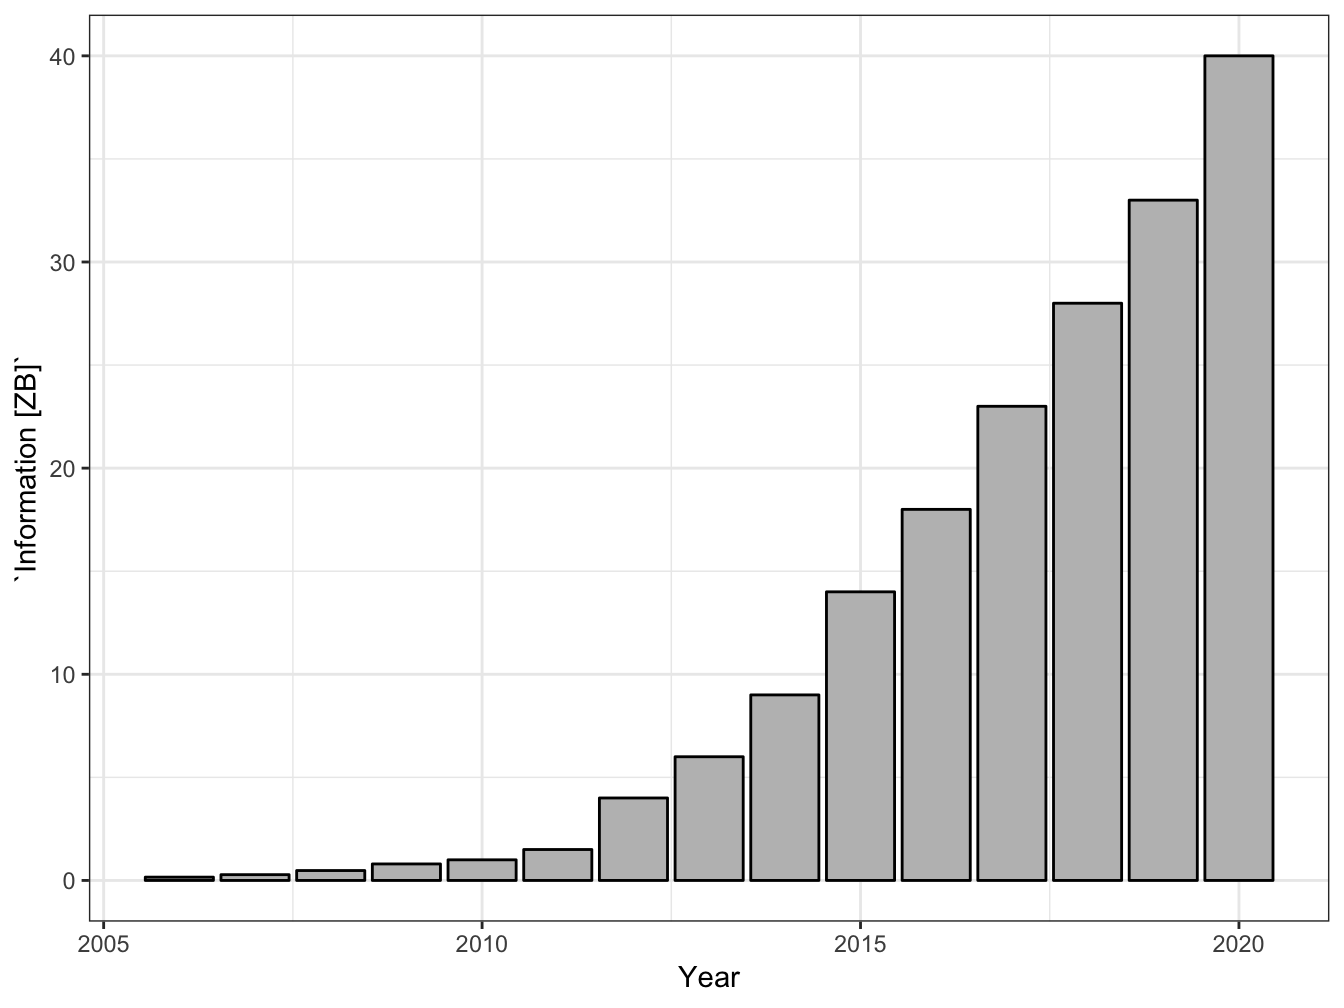
\includegraphics[width=0.6\linewidth]{thesis_source_files/figure-latex/biginfo-1} 

}

\caption{Hisogram of the eximated Zettabites of information produced from 2005 to 2020.}\label{fig:biginfo}
\end{figure}

\chapter{Scope of the Thesis}\label{scope-of-the-thesis}

\section{Sources of Information}\label{sources-of-information}

Documents written in natural language contains knowledge by design.
Their goal in fact is the explication of implicit knowledge
\citep[\citet{graesser1985structures}]{masters1992knowledge}. With the
growth of information of the last years also this kind of documents has
grown in number and there exist a huge opportunity for business to
manage this knowledge. The problem to address in order to take advantage
of this opportunity, is understanding which sources of information are
relevant to a certain company
\citep{larose2014discovering, chemchem2015data, kasemsap2015role}. It is
considered relevant all the information that helps the company building
knowledge as a tool to achieve their goals (both vision and mission).
Finding these sources requires a deep understanding of digital
technologies and of business acumen , skills that not every company can
have
\citep{hecklau2016holistic, davenport2012data, provost2013data, van2014data}.
To understand the practical implications of this issue, it has been
estimated that just a small portion of the digital universe has been
explored with the purpose of extracting competitive gain
\citep{data2012bigger}. The estimated percentage of untapped data is
25\% and it is going to rise to 33\% within 2020: it is likely that many
of the potential sources of valuable knowledge are not taken in to
consideration by companies and that a huge value is still hidden. This
untapped value can be potentially found everywhere in the info-verse:
users behaviors in social media, correlations among scientific studies,
overlaps between medical and sociological studies, beneath complex
analysis in legal documents and so on.

For these reasons an analytically process gains great value thanks to a
correct decision of which documents mine to extract knowledge. To
maximize this value the problem space has to be searched in term of
business relevant knowledge content of documents. Since this problem
space is huge (all the documents of which a company is stakeholder) in
the present thesis this decision has been taken a-priori ensuring a wide
set of document types in terms of their characteristics. These documents
are:

\begin{enumerate}
\def\labelenumi{\arabic{enumi}.}
\tightlist
\item
  \emph{Patents}
\item
  \emph{Scientific Papers}
\item
  \emph{Wikipedia}
\item
  \emph{Social Media}
\end{enumerate}

Patents has their core in technical information. Despite this, some
researchers \citep{bonino2010review} affirm that there is an increasing
variety of readers of patents: not only technician and researchers but
also marketers and designers who have grown an interest in patent
analysis. To our knowledge this thesis represent a first step the
direction of these potential readers. Papers are similar to patents in
terms of technical content but are not affected by the bias of being
legal documents. If this makes technical information easier to find, it
also brings a problem when there is the need of synthesizing the huge
information coming from a corpus of papers. Wikipedia is distant from
patents and papers. It (by design) contains encyclopedic and less
objective information, which comes in a semi-structured form. Due to the
bottom-up approach in which Wikipedia is developed, it has some
reliability shortages to take in to account. Finally social media
documents are far from the previous ones since they make use of a short,
subjective and colloquial lexicon. It is another of the challenges
addressed by this thesis to demonstrate that this sources contains
exploitable technical information too.

\section{Methods and Focus of the
Analysis}\label{methods-and-focus-of-the-analysis}

Thanks to the improvement in the Artificial Intelligence (AI) field,
\emph{Natural Language Processing} (NLP) has dramatically increased its
effectiveness in the last years \citep{russell2016artificial}. Now
powerful tools for the analysis of documents are available to every one
that has a little understating of programming
\citep[\citet{Kenneth2018spacyr},
\citet{Wijffels2018udpipe}]{Taylor2017Tidy}. For this reason, the
processes carried out in this thesis uses state of the art NLP
techniques that only in few cases has been deeply modified in the design
process. In other words the value of the output is not in the modified
NLP algorithm but on the whole process of knowledge extraction that goes
from the decision of which documents to analyze to the communication of
the results.

Furthermore, despite the golden ages of AI and NLP we are living in,
some problems this research area is trying to address are still having a
huge impact on companies \citep{hand2007principles, mining2006data}.

The first one is that the information overload is not manageable by
machines alone and thus there is the need of understating which are the
best practices in experts-machine interaction. In this context, it is
interesting to notice that the way companies incorporate knowledge in
their own artificial systems is drastically changed in the last 30
years. In fact, in the 1990s the main approach was knowledge
engineering: machine learned how to perform analysis tasks thanks to the
rules experts gave them. This idea has failed. In some contexts, it is
impossible representing knowledge with explicit expert-driven rules. For
this reason on the 2010s inductive revolution developed; machines are
used to extract knowledge from huge amounts of data in an inductive way.

This has led to a second major problem observed by literature: black
boxes or systems whose working mechanism are unknown, except input and
output. A recent paper \citep{pedreschi2018open} tries to clarify the
issue with black boxes and offers a few solutions. The authors point at
a way similar to reversing, in which a program is stimulated with
various inputs to study the outputs and understand its logic. In the
same way, to study the mechanisms of a machine-learning model, it is
possible to modify slightly the input only, and observe the result; or,
foresee the right input for the needed output. It is still cutting edge,
but it is already discussed and it is opening up to specific research,
such as explainable AI.

Considering these problems and considering the general goal of the
present thesis (i.e.~to extract and synthesize technical knowledge from
unstructured documents) we can state that we can not take aside the
design of processes, which can provide correct knowledge exchange
between human and machine, leading to:

\begin{itemize}
\item
  incorporate knowledge of the experts inside AI systems
\item
  experts' ability to use in their process of decision making,
  inductively generated knowledge of machines
\end{itemize}

\chapter{Approach}\label{approach}

\section{Design Science Paradigm}\label{introdesres}

Knowledge extraction systems are implemented within an organization for
the purpose of improving the probability for that organisation to reach
its goals. A wide literature exists on the design of these kind of
systems and the main focus comes from Information Systems (IS)
discipline. It is incumbent upon researchers in the IS to further
knowledge that aids in the productive application of information
technology to human organizations and their management
\citep{edit2002info} and to develop and communicate knowledge concerning
both the management of information technology and the use of information
technology for managerial and organizational purposes
\citep{Zmud1997edit}. Hevner et al. \citep{bichler2006design} argues
that acquiring such knowledge involves two complementary but distinct
paradigms: \emph{behavioral science} and \emph{design science}
\citep{march1995design}.

The \emph{behavioral-science paradigm} has its roots in the research
method of natural science
\citep{makadok2018practical, colquitt2007trends}. Its goal is to develop
and justify theories that explain (or predict) organizational phenomena
\citep{zahra2009maximizing} about the analysis, design, implementation,
management, and use of information systems. Such theories inform
researchers and companies of the interactions among humans, machines,
and organizations that must be managed if an information system has to
be effective. These theories interact with design decisions made with
respect to the system development methodology used
\citep{fini2018collaborative}.

The \emph{design-science paradigm} is a problem solving paradigm and has
its roots in engineering and the sciences of the artificial
\citep{simon1996sciences}. Its goal is to create innovations: define the
ideas, practices, technical capabilities, and products through which the
analysis, design, implementation, management, and use of information
systems can be effectively and efficiently accomplished
\citep{denning1997new, tsichritzis1997dynamics}. In this context the
researchers switches his goal: the artifacts that are created in the
research process are not exempt from natural laws or behavioral theories
but relies on existing kernel theories that are applied, tested,
modified, and extended through the experience, creativity, intuition,
and problem solving capabilities of the researcher
\citep{george2016big, madhavji2015big, markus2002design, walls1992building}.

Since Design science creates and evaluates IT artifacts intended to
solve identified organizational problems, the present thesis has as main
approach this second paradigm. In Design Science, artifacts are
represented in a structured form that may vary from software, formal
logic, and rigorous mathematics to informal natural language
descriptions. We will use all these representations at different level,
for the different applications described.

Furthermore the thesis has been developed following the guidelines of
design-science research. Hevner et al. \citep{bichler2006design} provide
a set of seven guidelines which help information systems researchers
conduct, evaluate and present design-science research. The guidelines
are summarised in table \ref{tab:introdesignscience}.

As previously discussed, design science is a problem solving paradigm.
The fundamental principle of design-science research is that is the
building and application of an artifact that permits to the researcher
to gain new knowledge and understanding of a design problem and its
solution. From this fundamental principle the seven guidelines are
derived. That is, design-science research must end and must have as goal
the \emph{creation of an innovative, purposeful artifact (Guideline 1)}
for a specified \emph{problem domain (Guideline 2)}. Because the
artifact has to be purposeful, researcher has to measure its utility for
the specified problem: this imply that \emph{evaluation of the artifact
is crucial (Guideline 3)}. Novelty is similarly crucial since the
artifact must \emph{solve an unsolved problem or solving a known problem
in a more effective or efficient manner (Guideline 4)}. In this way,
design-science research is differentiated from the practice of design
since artifact itself must be \emph{rigorously defined, formally
represented, coherent, and internally consistent (Guideline 5)}. The
process of design of the artificial and also artifact itself,
incorporates a search process whereby \emph{a problem space is
constructed and a mechanism posed or enacted to find an effective (not
necessarely otpimal) solution (Guideline 6)}. Finally, the results of
the \emph{design-science research must be communicated effectively
(Guideline 7)}.

The communication phase is crucial, and the results of a design science
based research has to be comprehensible and usable to:

\begin{itemize}
\tightlist
\item
  a technical audience (researchers who will extend them and
  practitioners who will implement them)
\item
  a managerial audience (researchers who will study them in context and
  practitioners who will decide if they should be implemented within
  their organizations).
\end{itemize}

\begin{table}

\caption{\label{tab:introdesignscience}Design-Science Research Guidelines}
\centering
\begin{tabular}[t]{>{}l>{\em\raggedright\arraybackslash}p{20em}}
\toprule
Guideline & Description\\
\midrule
Design as an Artifact & Design-science research must produce a viable artifact in the form of a construct, a model, a method, or an instantiation.\\
Problem Relevance & The objective of design-science research is to develop technology-based solutions to important and relevant business problems.\\
Design Evaluation & The utility, quality, and efficacy of a design artifact must be rigorously demonstrated via well-executed evaluation methods.\\
Research Contributions & Effective design-science research must provide clear and verifiable contributions in the areas of the design artifact, design foundations, and/or design methodologies.\\
Research Rigor & Design-science research relies upon the application of rigorous methods in both the construction and evaluation of the design artifact.\\
\addlinespace
Design as a Search Process & The search for an effective artifact requires utilizing available means to reach desired ends while satisfying laws in the problem environment.\\
Communication of Research & Design-science research must be presented effectively both to technology-oriented as well as management-oriented audiences.\\
\bottomrule
\end{tabular}
\end{table}

\section{Data Science Workflow}\label{data-science-workflow}

Many frameworks and models exists that describes the process of
knowledge extraction from data \citep[\citet{bellinger2004data},
\citet{ackoff1989data},
\citet{liew2007understanding}]{kanehisa2013data}. All this models brings
contribution to the literature but with a focus on the
\emph{behavioral-science paradigm}, thus with the goal to develop
theories about the analysis, design, implementation, management, and use
of data analysis systems.

For the present thesis we adopted a more actionable framework popular in
the field of data science: the Data Science Workflow
\citep{wickham2016r}. We adopted this model because is a generic
workflow that can be used as guideline to design any knowledge
extraction system. The workflow is represented in figure
\ref{fig:mainworkflow}.

The workflow is a model of the tools needed in a typical data science
project. Since data science is a huge field, and there's no way that a
model can master it, the goal of the model is to give a solid foundation
in the most important tools. These tools are used in every data science
project, but for most projects they are not enough. The tools
represented in the model has been chosen following a rough Pareto 80-20
rule \citep{pareto1971manual}.

The workflow is divided in the subsequent tasks:

\begin{itemize}
\item
  \emph{Import:} take data stored in a file, database, or web API, and
  load it into a computer.
\item
  \emph{Tidy:} Tidying data means storing it in a consistent form that
  matches the semantics of the data-set with the way it is stored. In
  brief, when the data is tidy, each column is a variable, and each row
  is an observation. Tidy data is important because the consistent
  structure lets focus on questions about the data and not in its shape.
\item
  \emph{Transform:} Transformation includes narrowing in on observations
  of interest, creating new variables that are functions of existing
  variables, and calculating a set of summary statistics.
\item
  \emph{Visualize:} Visualisation is a fundamentally human activity. A
  good visualisation will show unexpected information, or raise new
  questions about the data. A good visualisation might also hint that
  the hypothesis is wrong, or there is the need to collect different
  data. Visualisations can surprise, but do not scale particularly well
  because they require a human to interpret them.
\item
  \emph{Model:} Model is complementary to visualize. Once the hypothesis
  are sufficiently precise, a model can answer them. Models are a
  fundamentally mathematical or computational tool, so they generally
  scale well. Even when they don't, it's usually cheaper to buy more
  computers than it is to buy more brains. But every model makes
  assumptions, and by its very nature a model cannot question its own
  assumptions. That means a model cannot fundamentally surprise.
\item
  \emph{Communicate}: The last step is communication, an absolutely
  critical part of any project. As stated before communication phase is
  crucial, and the results of a design science based research has to be
  comprehensible and usable to a technical audience a managerial
  audience.
\item
  \emph{Program:} To design knowledge extraction tool programming is
  nowadays essential. There is no need to be an expert programmer to
  design effective knowledge extraction tool, but learning more about
  programming allows to automate common tasks, and solve new problems
  with greater ease.
\item
  \emph{Understand:} The greatest feature of a knowledge extraction
  system is not to detect the large trends- they are visible anyway; it
  is, rather, to detect weak signals, or information that initially
  appears with low frequency \citep{apreda2016functional}. These signals
  escape from traditional statistical detection techniques, exactly
  because it is difficult to distinguish them from pure statistical
  noise. It is hard to distinguish weak-signals from noise only using
  algorithms: understanding the problem to be solved and having domain
  expertise is essential. For this reason \emph{understand} is not only
  part of the process of analysis, but is maybe the most important task
  with respect to the present thesis.
\end{itemize}

A full state of the art on all of these tasks as been conducted in
section \ref{sotatools}.

\begin{figure}

{\centering 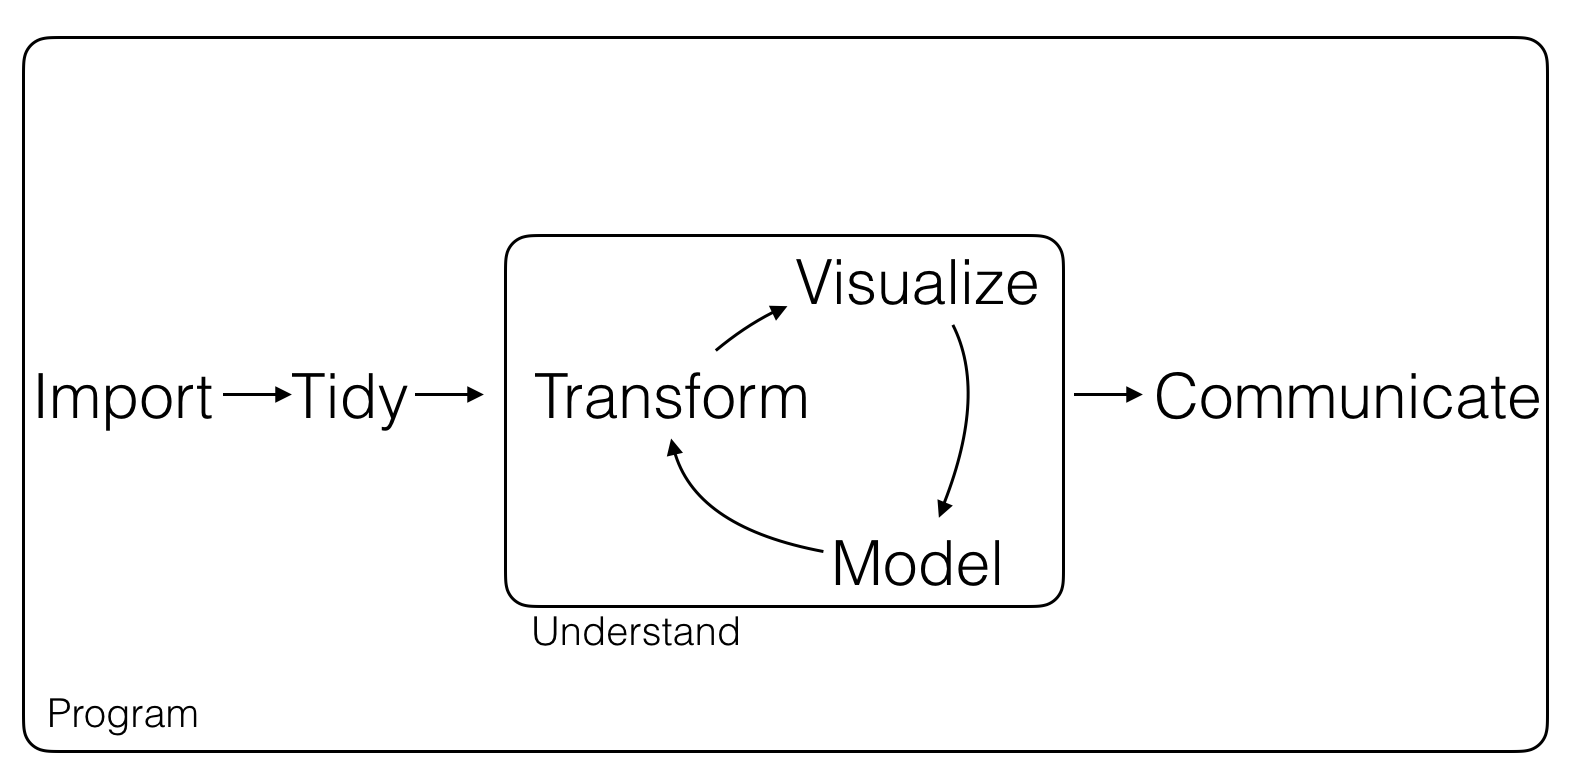
\includegraphics[width=0.8\linewidth]{_bookdown_files/figures/main_work_flow} 

}

\caption{A general workflow for the process of data analysis. Readapted from Wickham (2016)}\label{fig:mainworkflow}
\end{figure}

\chapter*{Structure and Rationale}\label{structure-and-rationale}
\addcontentsline{toc}{chapter}{Structure and Rationale}

The selected documents to analyze, the exploitation of Natural Language
Processing Techniques , the Design Science Approach and the Data Science
Workflow helps to explain the structure of this thesis, since the
decision of using these paradigm and tools had a direct impact on its
form and content. The thesis is in fact structured as follow:

\begin{itemize}
\item
  \emph{Part Number 2 ``State of the Art''} makes a review of tools and
  techniques for Natural Language Processing and shows the documents
  used for knowledge extraction. In particular, the analysis of
  technical documents require the design of processes that rely both on
  Natural Language Processing techniques and on technical field experts.
  While the first techniques are codified and explicit, the second are
  sometimes implicit and always hard to systematize. In the State of the
  Art these two groups of techniques are treated in the same way to give
  to the reader a systematic literature review on these topics.
  Furthermore it is important to define the value in terms of new
  knowledge that documents can bring to companies. The goal of this
  state of the art is to demonstrate that a large literature on
  Techniques able to solve the problems described in section
  \ref{introproblems} exists, but weak or no effort exist in the
  literature in the systemic integration of these tools and in the
  design of holistic methods to solve these problems.
\item
  \emph{Part Number 3 ``Methods and Results''} is the core Part of the
  thesis. This part describes the methods and processes designed for the
  analysis of technical documents following the guidelines of design
  research described in section \ref{introdesres}. Since design research
  is a problem solving paradigm, each chapter (focalised on a different
  kind of document) starts with a brief description of the field of
  application of the method and with the framing of the problem to be
  solved. Then the methodology to solve the problem is described with
  the goal of being clear to a technical audience and a managerial
  audience. Each chapter closes with the results description that proves
  the utility, quality, and efficacy of the design artifact.
\item
  \emph{Part Number 4 ``Applications of the Results''} is a collection
  of projects that describes the applications and results of the methods
  designed in \emph{Part 3 ``Methods and Results''}. The goal, again
  following the the guidelines of design research
  \citep{bichler2006design}, is to provide clear and verifiable
  contributions in the areas of the design artifact, design foundations,
  and/or design methodologies.
\item
  \emph{Part Number 5 ``Conclusions''} summarises the thesis, and its
  possible future developments. The thesis ends giving a more
  descriptive-science view of the results. In this last part we focus on
  a general method that has proven to be effective in the major part of
  the designs of the present thesis: \textbf{lexicons design}.
\end{itemize}

\part{State of the Art}\label{part-state-of-the-art}

The analysis of technical documents require the design of processes that
rely both on Natural Language Processing techniques and on technical
field expertise. While the first techniques are codified and explicit,
the second are sometimes implicit and always hard to systematize. In
this section i treat these two groups of techniques in the same way to
give to the reader a systematic literature review on these topics. This
chapter can be seen as a background chapter as it illustrates the
information that the reader should know to understand the rest of the
dissertation. Furthermore it is important to define the value in terms
of new knowledge that documents can bring to companies. For this reason
the chapter of this part has the subsequent structure:

\begin{itemize}
\item
  At a first level there are two sections \ref{sotatools} and
  \ref{sotadocuments}, reviewing respectively the processes of
  \emph{programming and Natural Language Processing} and the
  \emph{documents};
\item
  Section \ref{sotatools} has a subsection for each of the \emph{phases}
  showed in figure \ref{fig:mainworkflow}. These subsections goes from
  \ref{sotatoolsprogram} to \ref{sotatoolscomunicate};
\item
  Each subsection from \ref{sotatoolsprogram} to
  \ref{sotatoolscomunicate} contains the relative Natural Language
  Processing \emph{task} that are relevant for the analysis of technical
  documents, for example Document Retrieval
  \ref{sotatoolsimportretrieval}, Part-Of-Speech-Tagging;
  \ref{sotatoolstransformpos} or Named Entity Recognition
  \ref{sotatoolsmodelner}.
\item
  Each task subsection describes the relevant \emph{techniques} to
  perform that task. I use the word techniques to include mainly
  algorithms and procedures but also more generic methods or frameworks;
\item
  Finally, section \ref{sotadocuments} has a subsection for each of the
  analyzed technical \emph{documents}. These subsections goes from
  \ref{sotadocumentspatents} to \ref{sotadocumentstwitter}.
\end{itemize}

The goal of this state of the art is to demonstrate that a large
literature on Techniques able to solve the problems described in section
\ref{introproblems} exists, but week or no effort exist in the
literature in the systemic integration of these tools.

\chapter{Phases, Tasks, and Techniques}\label{sotatools}

In this section I make a review of the most important techniques for
Natural Language Processing in the context of technical documents
analysis. The techniques (mainly algorithms) are grouped in phases
(Import, Tidy, Transform, Model, Visualize, Communicate) showed in
figure \ref{fig:mainworkflow} and each phases is dived in the NLP tasks
that are the most important for the analysis of technical documents.
This standard process has been disclosed in the framework of the
tidyverse \citep{wickham2016r}.

\section{Program}\label{sotatoolsprogram}

Programming is a key activity to perform in order to effectively and
efficiently perform text mining. It is not a phases per se because each
phase is implemented trough programming. It is critical that an analysts
has in mind the need of maximizing the probability that their analysis
is reproducible, accurate, and collaborative. This goals can be reached
only trough programming. The most used programming languages for text
mining and natural language processing are R \citep{r2008} and Python
\citep{py95}. R and Python are both open-source programming languages
with a large community of developers, and new libraries or tools are
added continuously to their respective catalog. R is mainly used for
statistical analysis and data science while Python is a more general
purpose programming language.

R has been developed by Academics and statisticians over two decades. R
has now one of the richest ecosystems to perform data analysis and there
are around 12000 packages available in CRAN (open-source repository of
R). The rich variety of libraries makes R the first choice for
statistical analysis. Another cutting-edge difference between R and the
other statistical products is R-studio. RStudio is a free and
open-source integrated development environment (IDE) for R. It includes
a console, syntax-highlighting editor that supports direct code
execution, as well as tools for plotting, history, debugging and
workspace management. Finally, it is widely recognized the great
performances that R has for data visualisation and communication.

Python can pretty much do the same tasks as R: data wrangling,
engineering, feature selection web scrapping, app and so on. Anyway,
Python has great performances in the deployment and implementation of
machine learning at a large-scale. Furthermore, Python codes are easier
to maintain and more robust than R.

\section{Import}\label{sotatoolsimport}

The first activities to perform in a text mining pipeline is to find all
the documents that contains useful information for the analysis and then
import the corpus (the set of documents) in to the computer program. The
present section is thus focused on techniques for document retrieval
\ref{sotatoolsimportretrieval} and on the most popular documents digital
formats \ref{sotatoolsimportformat}.

\subsection{Document Retrieval}\label{sotatoolsimportretrieval}

Document retrieval is the process of matching a user query against a set
of documents. A document retrieval system has two main tasks:

1- Find the documents that are relevant with respect to the user queries
2- Measure the relevance of the matching results

Building a query means to use field specific knowledge and logical rules
to write a text string that is the composition of keywords and Boolean
operators. The set of keywords (single words or phrases) is chosen in
such a way that these are likely to be contained in the searched
documents. Boolean operators can also be used to increment the
performance of the query. The AND operator, for example is used to
retrieve all the document that contains both of the terms at the left
and the right of it, OR for document that contains at least one of the
two words. Another important tool for making a good query are regular
expressions. Regular expression (regexp) is a language for specifying
text search strings, an algebraic notation for characterizing a set of
strings. This language widely used in modern word processor and text
processing tools. A regular expression search function will search
through the corpus, returning all texts that match the pattern. For
example, the Unix command-line tool grep takes a regular expression and
returns every line of the input document that matches the expression. To
evaluate the performance of a query is useful to understand the concepts
of precision and recall.

Recall is the ratio of relevant results returned to all relevant
results. Precision is the number of relevant results returned to the
total number of results returned. Due to the ambiguities of natural
language, full-text-search systems typically includes options like stop
words to increase precision. Stop-words are words that filter all the
document which contains them. On the other side, stemming to increase
recall \ref{sotatoolstransformstemming}. The trade-off between precision
and recall is simple: an increase in precision can lower overall recall,
while an increase in recall lowers precision \citep{yuwono1996search}.
Usually when a user performs a query, the main problem are false
positives (the results that are returned by the systems but are not
relevant to the user). False positives has a negative impact on the
precision of the query. The retrieval of irrelevant documents is
particularly strong for technical documents due to the inherent
ambiguity of technical language. For this reason to understand and to
use the rules of query building are fundamental to the technical
document analysis, since without a good query is rare to have a good set
of documents to analyze.

\subsection{Documents Format}\label{sotatoolsimportformat}

For the purpose of the present thesis documents are considered in a
digital format, and there is no need to read it from a analogical
source. From the computer science point of view, text is a
human-readable sequence of characters and the words they form that can
be encoded into computer-readable formats. There is no standard
definition of a text file, though there are several common formats. The
most common types of encoding are:

\begin{itemize}
\item
  ASCII, UTF-8: plain text formats
\item
  .doc for Microsoft Word: Structural binary format developed by
  Microsoft (specifications available since 2008 under the Open
  Specification Promise)
\item
  HTML (.html, .htm): open standard, ISO from 2000
\item
  Office Open XML .docx: XML-based standard for office documents
\item
  OpenDocument .odt: XML-based standard for office documents
\item
  PDF: Open standard for document exchange. ISO standards include PDF/X
  (eXchange), PDF/A (Archive), PDF/E (Engineering), ISO 32000 (PDF),
  PDF/UA (Accessibility) and PDF/VT (Variable data and transactional
  printing). PDF is readable on almost every platform with free or open
  source readers. Open source PDF creators are also available.
\item
  Scalable Vector Graphics (SVG): Graphics format primarily for
  vector-based images.
\item
  TeX: Popular open-source typesetting program and format. First
  successful mathematical notation language.
\end{itemize}

For the R software there exist many packages that helps to import
documents in several formats \citep{readr2017r}.

\section{Tidy}\label{sotatoolstidy}

After that data are imported they have to be processed in such a way
that it would be possible to perform the main task of data analysis
(transformation, modelling and visualisation). This task of tidying data
(usually referred to as data pre-processing) can be very time expensive,
so it is important to have clear methods and techniques to perform this
task.

Tidy data sets have structure and working with them is easy; they're
easy to manipulate, model and visualize \citep{wickham2014tidy}. Tidy
data sets main concept is to arrange data in a way that each variable is
a column and each observation (or case) is a row. The characteristics of
tidy data can be thus summarised as the points \citep{leek2015elements}:

\begin{itemize}
\tightlist
\item
  Each variable you measure should be in one column
\item
  Each different observation of that variable should be in a different
  row
\item
  If you have multiple tables, they should include a column in the table
  that allows them to be linked
\end{itemize}

The main advantages of structuring the data in this way is that a
consistent data structure make it easier to use the tools (programs)
that work with it because they have an underlying uniformity. This lead
to an advantage in reproducibility of code.

In the context of the present Thesys, the Tidy task mean applying this
process to text. It is clear that to tidy unstructured information is
harder then to tidy structured data \citep{silge2016tidytext}. On the
other side, using tidy data principles can make many text mining tasks
easier, more effective, and consistent with tools already in wide use.
Treating text as data frames of individual words allows us to
manipulate, summarize, and visualize the characteristics of text easily
and integrate natural language processing into effective workflows
already used.

Tidy text format is designed as being a table with one-token-per-row. A
token unit of text that is meaningful for the analysis to be performed
(for example letters, words, n-gram, sentences, or paragraphs ).
Tokenization is the process of splitting text into tokens. This
one-token-per-row structure is in different from the ways documents are
often stored in current analyses, mainly strings or document-term
matrix. The term document matrix has each corpus word represented as a
row with documents as columns. The document term matrix is the
transposition of the TDM so each document is a row and each word is a
column. The term document matrix or document term matrix is the
foundation of bag of words text mining. The bag-of-words model is a
simplifying representation of documents: a text is represented as the
bag (multiset) of its words, disregarding grammar and even word order
but keeping multiplicity \citep{mctear2016conversational}.

\section{Transform}\label{sotatoolstransform}

Transforming in the context of Natural Language Processing is what in
computational linguistic is called text normalization. Normalizing text
means converting it to a more convenient, standard form. Most of the
task of technical document analysis in fact relies on first separating
out or tokenizing sentences and words, strip suffixes from the end of
the word, determining the root of a word or transform the text using
regular expressions.

\subsection{Sentence Splitting}\label{sotatoolstransformsentencesplit}

The analysis of technical documents require as first process, that the
input text is segmented in sentences. Since documents do not encode this
information in a non ambiguous manner (using dots) due to common
abbreviations (e.g.: ``Mr., Dr.''), a sentence splitting process that
does not rely only on a trivial \emph{dot based} rule is required. This
issue in the technical documents domain is even more problematic due to
the presence of formulas, numbers, chemical entity names and
bibliographic references. Furthermore, since sentence splitting is one
of the first processes of an NLP pipeline, errors in this early stage
are propagated in the following steps causing a strong decrease for what
concerns their accuracy. One of the most advanced techniques are machine
learning techniques: given a training corpus of properly segmented
sentences and a learning algorithm, a statistical model is built. By
reusing the statistical model, the sentence splitter is able to split
sentences on texts not used in the training phase. ItalianNLP lab
systems uses this approach
\citep{dell2009ensemble, attardi2009reverse, attardi2009accurate}. For
this reason this algorithm is used for the most of the application
presented in this Thesis.

\subsection{Tokenization}\label{tokenization}

Since documents are unstructured information, these has to be divided
into linguistic units. The definition of linguistic units is
non-trivial, and more advanced techniques can be used (such as n-gram
extraction) but most of the times these are words, punctuation and
numbers. English words are often separated from each other by white
space, but white space is not always sufficient. Solving this problems
and splitting words in well-defined tokens defined as tokenization. In
most of the application described in the present Thesis, the tokenizer
developed by the ItalianNLP lab was integrated
\citep{dell2009ensemble, attardi2009reverse, attardi2009accurate}. This
tokenizer is regular expression based: each token must match one of the
regular expression defined in a configuration file. Among the others,
rules are defined to tokenize words, acronyms, numbers, dates and
equations.

\subsection{Stemming}\label{sotatoolstransformstemming}

Stemming is a simpler but cruder methodology for chopping off of
affixes. The goal of stemming is reducing inflected (or sometimes
derived) words to their word stem, base or root form. The stem of a word
and its morphological root do not need to be identical; it is sufficient
that related words map to the same stem, even if this stem is not a
valid root. One of the most widely used stemming is the simple and
efficient Porter algorithm \citep{porter1980algorithm}.

\subsection{Lemmatisation}\label{sotatoolstransformlemmatisation}

Lemmatization is the task of determining the root of a words. The output
allow to find that two words have the same root, despite their surface
differences. For example, the verbs \emph{am}, \emph{are}, and \emph{is}
have the shared lemma \emph{be}; the nouns \emph{cat} and \emph{cats}
both have the lemma \emph{cat}. Representing a word by its lemma is
important for many natural language processing tasks. Lemmatisation in
fact diminish the problem of sparsity of document-word matrix.
Furthermore lemmatisaion is important for document retrieval
\ref{sotatoolsimportretrieval} web search, since the goal is to find
documents mentioning motors if the search is for motor. The most recent
methods for lemmatization involve complete morphological parsing of the
word \citep{hankamer1989morphological}.

\subsection{Words importance metrics}\label{sotatoolstransformwi}

Once that a document has been tokenized and the tokens has been
transformed, an analyst usually wants to measure how important a word is
to a document in a collection or corpus. Some of the metrics adopted
are:

\begin{itemize}
\tightlist
\item
  \emph{Term Frequency}: the number of times that a term occurs in
  document.
\item
  \emph{Boolean frequency}: 1 if the term occurs in the document and 0
  otherwise;
\item
  \emph{Term frequency adjusted for document length}: is raw count
  normalized for the number of words contained in the document
\item
  \emph{Logarithmically scaled frequency}: is raw count normalized for
  the natural logarithm of one plus the number of words contained in the
  document
\item
  \emph{Inverse document frequency}: is the logarithmically scaled
  inverse fraction of the documents that contain the word, obtained by
  dividing the total number of documents by the number of documents
  containing the term, and then taking the logarithm of that quotient.
  It is a measure of how much information the word provides, that is,
  whether the term is common or rare across all documents.
\item
  \emph{Term frequency--Inverse document frequency}: the product between
  \emph{term frequency and inverse document frequency}. A high weight in
  tf--idf is reached by a high term frequency (in the given document)
  and a low document frequency of the term in the whole collection of
  documents; the weights hence tend to filter out common terms.
\end{itemize}

\subsection{Part-of-Speech Tagging}\label{sotatoolstransformpos}

The part of speech plays an central role in technical document analysis
since it provides very useful information concerning the morphological
role of a word and its morphosyntactic context: for example, if a token
is a determiner, the next token is a noun or an adjective with very high
confidence. Part of speech tags are used for many information extraction
tools such as named entity taggers (see section \ref{sotatoolsmodelner})
in order to identify named entities. In typical named entity task these
are people and locations since tokens representing named entities follow
common morphological patterns (e.g.~they start with a capital letter).
For the application to technical documents, technical entities (like the
possible failures of a manufact) becomes more relevant. In this context
a correct part-of-speech tagger becomes even more important since
morphosyntactical rules can not be used. In addition part of speech tags
can be used to mitigate problems related to polysemy since words often
have different meaning with respect to their part of speech (e.g.
``track'', ``guide''). This information is extremely valuable in patent
analysis, and some patent tailored part-of-speech tagger has been
designed (see section \ref{sotadocumentspatents}). The literature on
pos-tagger is huge, and goes behind the scope of the present thesis to
make a complete review. In most of the application presented in this
work, was employed the ILC postagger \citep{attardi2006experiments}.
This postagger uses a supervised training algorithm: given a set of
features and a training corpus, the classifier creates a statistical
model using the feature statistics extracted from the training corpus.

\section{Model}\label{sotatoolsmodel}

The goal of a model is to provide a simple low-dimensional summary of a
dataset \citep{wickham2016r}. Ideally, the model will capture patterns
generated by the phenomenon of interest (true signals), and ignore
random variations (noise). A good model at the same time is able to
capture the weak signals that cab be easily confounded with noise. These
information is particularly valuable in the context of technical
document analysis, where great technical insight could come weak
quasi-invisible signals. \citep{james2013introduction}

Probabilistic models are widely used in text mining nowadays, and
applications range from topic modeling, language modeling, document
classification and clustering to information extraction. The present
section contains a review of the most used methods used to model textual
information.

\subsection{N-Grams}\label{sotatoolstransformngrams}

An n-gram is a sequence of N n-gram words: a 2-gram (or bigram) is a
two-word sequence of words like ``credit card'', ``3d printing'', or
''printing machine'', and a 3-gram (or trigram) is a three-word sequence
of words like ``3d printing machine''. Statistical model can be used to
extract the n-grams contained in a document. A first approach has the of
predicting the next item in a sequence in the form of a (n − 1)--order
Markov model\citep{lafferty2001document}. The algorithm begin with the
task of computing P(w\textbar{}h), the probability of a word w given a
word h.The way to estimate this probability is using relative frequency
counts. To do that the algorithms count the number of times h is
followed by the w. With a large enough corpus it is possible to build
valuable models, able to extract n-grams
\citep{bellegarda2004statistical}. While this method of estimating
probabilities directly from counts works for many natural language
applications, in many cases a huge dimension of the corpus does make the
model useful, and this is particularly true for technical documents
\citep{brants2012large}. This is because technical language has a strong
ratio of evolution; as new artifact are invented, new chunks are created
all the time, and has no sense to continuously count every word
co-occurrence to update our model\citep{gibson1994tools}. A more useful
method for chunk extraction fro technical document uses
part-of-speech-tagging and regular expression. Once a document is
pos-taggerd each word is associated whit a particular part of speech:
each sentence is represented as a sequence of part-of-spech. Once this
representation is ready, it is possible to extract only certain
sequences of part-of-speeches, the ones that whit an high level of
confidence are n-grams.

\subsection{Document Classification}\label{sotatoolsmodeldocclass}

Classification is a general process that has the goal of taking an
object, extract features, and assign to the observation one of a set of
discrete classes. This process is largely used for documents
\citep{borko1963automatic} and there exist many methods for document
classification \citep{aggarwal2012survey}.

Regardless of technological sector, most organizations today are facing
the problem of overload of information. When it comes to classify huge
amount of documents or to separate the useful documents from the
irrelevant, document classification techniques can reduce the process
cost and time.

The simplest method for classifying text is to use expert defined rules.
These systems are called expert systems or knowledge engineering
approach. Expert rule-based systems are programs that consist of rules
in the IF form condition THEN action (if condition, then action). Given
a series of facts, expert systems, thanks to the rules they are made of,
manage to deduce new facts. The expert systems therefore differ from
other similar programs, since, by referring to technologies developed
according to artificial intelligence, they are always able to exhibit
the logical steps that underlie their decisions: a purpose that, for
example, is not feasible from the human mind or black box-systems. There
are many type of documents for which expert based classifiers constitute
a state-of-the-art system, or at least part of it. Anyway, rules can be
useless in situations such as: - data change over time - the rules are
too many and interrelated

Most systems of documents classification are instead done via supervised
learning: a data set of input observations is available and each
observation is associated with some correct output (training set). The
goal of the algorithm is to build a static model able to learn how to
map from a new observation (test set) to a correct output. The
advantages of this approach over the knowledge engineering approach are
a very good effectiveness, considerable savings in terms of expert labor
power, and straightforward portability to different domains.

In the supervised document classification process, is used a training
set of N documents that have each been typically hand-labeled with a
class: (d1, c1),\ldots{}.,(dN, cN). I say typically, because other less
expensive methods could be designed, as it will be shown for the task of
Named Entity Recognition (another supervised learning task, that
classifies words instead of documents \ref{sotatoolsmodelner}). The goal
of the supervised document classification task is to learn a statistical
model capable of assign a new document d to its correct class c ∈ C.
There exist a class of these classifier, probabilistic classifiers, that
additionally will tell us the probability of the observation being in
the class.

Many kinds of machine learning algorithms are used to build classifiers
\citep{aggarwal2012survey}, such as:

\begin{itemize}
\item
  \emph{Decision Tree Classifiers}: Decision tree documents classifier
  are systems that has as output a classification tree
  \citep{sebastiani2002machine}. In this tree internal nodes are terms
  contained in the corpus under analysis, branches departing are labeled
  by the weight (see section \ref{sotatoolstidy}) that the term has in
  the test document, and leafs are labeled by categories. There exists
  many methods to automatically learn trees from data. A tree can be
  build by splitting the data source into subsets based on an test
  feature. This process is repeated on each derived subset in a
  recursive manner called recursive partitioning. The recursion is
  completed when the subset at a node has all the same value of the
  target variable, or when splitting no longer adds value to the
  predictions.
\item
  \emph{Rule Based Classifiers}: Rule-based classifiers are systems in
  which the patterns which are most likely to be related to the
  different classes are extracted from a set of test documents. The set
  of rules corresponds to the left hand side to a word pattern, and the
  right-hand side to a class label. These rules are used for the
  purposes of classification. In its most general form, the left hand
  side of the rule is a Boolean condition, which is expressed in
  Disjunctive Normal Form (DNF). However, in most cases, the condition
  on the left hand side is much simpler and represents a set of terms,
  all of which must be present in the document for the condition to be
  satisfied \citep{yang2004building}.
\item
  \emph{Support Vector Machines (SVM) Classifiers}: SVM Classifiers
  attempt to partition the data space with the use of linear or
  non-linear delineations between the different classes. The main
  principle of SVM algorithm is to determine separators in the feature
  space which can best separate the different classes
  \citep{joachims1998text, manevitz2001one}.
\item
  \emph{Baeysian Classifiers}: Bayesian classifiers build a
  probabilistic classifier based on modeling the underlying word
  features in different classes. The idea is then to classify documents
  using the posterior probability of the documents belonging to the
  different classes on the basis of the word presence in the documents
  \citep{pop2006approach}.
\item
  \emph{Neural Network Classifiers}: The basic unit in a neural network
  is a neuron. Each neuron receives a set of inputs, which are denoted
  by the vector \emph{Xi}, which are the values of the feature vector
  for a certain instance. Each neuron is also associated with a set of
  weights, which are used in order to compute a function of its inputs.
  Neural Networks Classifier are able, thank to a process called
  learning phase, to adjust their weights in such a way that the
  function is able to effectively classify new instances. Neural
  networks are nowadays one of the best method for documents
  classification, and are used in a wide variety of applications
  \citep{manevitz2007one}. Great performances has also been reached by
  deep neural networks, which are neural networks whit a large number o
  neurons arranged in multiple layers
  \citep{lai2015recurrent, kim2014convolutional}.
\end{itemize}

\subsection{Sentiment Analysis}\label{sotatoolsmodelsentanal}

Sentiment analysis techniques are algorithms able to measure from text,
people's opinions and emotions toward events, topics, products and their
attributes \citep{pang2008opinion}. For example, businesses
(particularly marketeers) are interested in finding costumers opinions
about their products and services.

Thanks to the growth of social media (forums, blogs and social
networks), individuals and organizations are producing a huge quantity
of their written opinion. This has make it possible to scholars to study
this phenomena and to develop many different and effective sentiment
analysis techniques \citep{liu2012survey}. In the past decade, a
considerable amount of research has been done by scholars and there are
also numerous commercial companies that provide opinion mining services.
However, measuring sentiment in documents and distilling the information
contained in them remains a challenging task because of the diversity of
documents from which is possible to extract sentiment.

The approaches to perform sentiment analysis are many. Among all, the
most interesting for technical documents analysis are:

\begin{itemize}
\item
  \emph{Dictionary Base Approaches} : This approach has the aim of
  collecting words that are clues for positive or negative sentiment. In
  literature these words are called opinion words, opinion-bearing words
  or sentiment words. Examples of positive opinion words are: good, nice
  and amazing. Examples of negative opinion words are bad, poor, and
  terrible. Collectively, they are called the opinion lexicon. The most
  simple and widely used techniques to produce a dictionary of opinion
  words is based on bootstrapping using a small set of seed opinion
  words and an online dictionary such as WordNet
  \citep{miller1995wordnet}. The works that used this approach
  \citep{hu2004mining, kim2004determining}, adopts a process that
  consist in two phases: first collect set of opinion words manually,
  then grow this set by searching in the WordNet for their synonyms and
  antonyms. The process stops when no more new words are found. After
  that a manual inspection can be carried out to remove and/or correct
  errors. Scholars has developed several opinion lexicons
  \citep{ding2008holistic, baccianella2010sentiwordnet, hu2004mining, philip1966general, wiebe1999development}
  The lexicon based approach has the characteristic of being strongly
  context specific. This is an advantage when the goal is to design a
  method able to extract sentiment in a specific context
  \citep{chiarello2017product}, but is a major shortcoming if the goal
  is to design a general purpose method.
\item
  \emph{Supervised Learning Approaches}: Sentiment analysis can be
  formulated as a document classification problem with three classes:
  positive, negative and neutral\citep{mullen2004sentiment}. Training
  and test sets of documents are typically collected from product
  reviews, movies reviews or are created by scratch using manual
  annotation. Any learning algorithm can be applied to sentiment
  classification (naive Bayesian classification, and support vector
  machines \citep{prabowo2009sentiment}). The crucial phase for
  Supervised Learning sentiment analysis is the features presentation of
  the data. It was shown \citep{pang2002thumbs} that using uni-grams (a
  bag of individual words) as features in classification performed well
  with either naive Bayesian or SVM. Subsequent research used many more
  features and techniques in learning \citep{pang2008opinion}.
\end{itemize}

\subsection{Text Clustering}\label{sotatoolsmodelnetanal}

The goal of clustering methods is to find groups of similar objects in
the data thanks to the measure of a similarity function
\citep{jain1988algorithms, kaufman2009finding}. Clustering techniques
are widely applied in the text domain, where the objects of the
clustering can be documents (at different level of granularity) or
terms. In the context of technical documents analysis Clustering is
especially useful documents retrieval
\citep{anick1997exploiting, cutting1993constant}. Clustering problems
are studied widely outside the text domain. Methods for clustering have
been developed focusing on quantitative/non-textual data
\citep{guha1998cure, han2001spatial, zhang1996birch}.

In the context of text analysis, the problem of clustering finds
applicability for a number of tasks, such as Document Organization and
Browsing \citep{cutting2017scatter}, Corpus Stigmatization using
documents maps \citep{schutze1997projections} or word clusters
\citep{baker1998distributional, bekkerman2001feature}. It is useful also
to use a Soft clustering approach, that associates each document with
multiple clusters with a given probability.

However, standard techniques for cluster analysis (k-means or
hierarchical clustering) do not typically work well for clustering
textual data in general or more specific technical documents. This is
because of the unique characteristics of textual data which implies the
design of specialized algorithms for the task.

The distinguishing characteristics of the text representation are the
following \citep{aggarwal2012survey}:

\begin{itemize}
\item
  There is a problem of course of dimensionality. The dimensionality of
  the bug-of-words representation is very large and the underlying data
  is sparse. In other words, the lexicon from which the documents are
  drawn may be of the order of millions, but a given document may
  contain only a few hundred words.This problem is even more serious for
  technical documents in which the lexicon is even more large.
\item
  The words are correlated with one another and thus the number of
  concepts (or principal components) in the data is much smaller than
  the feature space. This necessitates the careful design of algorithms
  which can account for word correlations in the clustering process.
\item
  The number of words (or non-zero entries) in the different documents
  may vary widely. Therefore, it is important to normalize the document
  representations appropriately during the clustering task.
\end{itemize}

The problems of sparsity and high dimensionality necessitate the design
of specific algorithms text processing. The topic has been heavily
studied in the information retrieval literature where many techniques
have been proposed \citep{ricardo2011modern}.

\subsection{Named Entity Recognition}\label{sotatoolsmodelner}

Named Entity Recognition is the task of identifying entity names like
people, organizations, places, temporal expressions or numerical
expressions. An example of an annotated sentence for a NER extraction
system tailored for user entity extraction from patents, is the
following:

\emph{Traditionally, guitar players or players of other stringed
instruments may perform in any of a number of various positions, from
seated, with the stringed instrument supported on the leg of the
performer, to standing or walking, with the stringed instrument
suspended from a strap.}

Methods and algorithms to deal with the entity extraction task are
different, but the most effective are the ones based on supervised
methods. Supervised methods tackle this task by extracting relevant
statistics from an annotated corpus. These statistics are collected from
the computation of features values, which are strong indicators for the
identification of entities in the analyzed text. Features used in NLP
for NER purposes are divided in two main categories: - Linguistically
motivated features, such as n-gram of words (sequences of n words),
lemma and part of speech - External resources features as, for example,
external lists of entities that are candidates to be classified in the
extraction process.

The annotation methods of a training corpus can be of two different
kinds: human based, which is time expensive, but usually effective in
the classification phase; automatically based, which can lead to
annotation errors due to language ambiguity. For instance driver can be
classified both as a user (the operator of a motor vehicle), or not a
user (a program that determines how a computer will communicate with a
peripheral device). Different training algorithms, such as Hidden Markov
Models \citep{eddy1996hidden}, Conditional Random Fields (CRF)
\citep{lafferty2001conditional} Support Vector Machines (SVM)
\citep{hearst1998support}, or Bidirectional Long Short Term Mermory-CRF
Neural Networks \citep{lample2016neural, misawa2017character} are used
to build a statistical model based on features that are extracted from
the analyzed documents in the training phase.

\subsection{Topic Modelling}\label{sotatoolsmodeltopicmodel}

Topic modeling is a form of dimension reduction that uses probabilistic
models to find the co-occurrence patterns of terms that correspond to
semantic topics in a collection of documents
\citep{crain2012dimensionality}. To understand topic modelling it is
useful to understand its differences with clustering
\ref{sotatoolsmodelnetanal} and the problem they both solves: the course
of dimensionality. Both these techniques has in fact the goal of
representing documents in such a way that they reveals their internal
structure and interrelations.

Clustering measures the similarity (or dissimilarity) between documents
to place documents into groups. Representing each document by
considering the belonging to a group, clustering induces a
low-dimensional representation for documents. However, it is often
difficult to characterize a cluster in terms of meaningful features
because the clustering is independent of the document representation,
given the computed similarity. Topic modeling integrates soft clustering
(assigning each element to a cluster with a given probability and not
with a Boolean variable) with dimension reduction. Each document is
associated with a number of latent topics: a topic can be seed as both
document clusters and compact group of words identified from a corpus.
Each document is assigned to the topics with different weights: this
feature can be seen both as the degree of membership in the clusters, as
well as the coordinates of the document in the reduced dimension space.
The result is an understandable representation of documents that is
useful for analyzing the themes in documents. Latent Dirichlet
allocation (LDA) is a particularly popular method for fitting a topic
model \citep{blei2003latent}. It treats each document as a mixture of
topics, and each topic as a mixture of words. This allows documents to
``overlap'' each other in terms of content, rather than being separated
into discrete groups, in a way that mirrors typical use of natural
language.

\section{Visualize}\label{sotatoolsvisualize}

Traditionally, statistical training has focused primarily on
mathematical derivations and proofs of statistical tests: the process of
developing the outputs (the paper, the report, the dashboard, or other
deliverable) is less frequently analyzed. This problem influences also
text mining \citep{parker2017opinionated}. One of the most studied
problems of output production is data visualisation. Data visualisation
involves the creation and study of the visual representation of data
\citep{friendly2001milestones}. Data visualization uses statistical
graphics, plots, information graphics and other tools to communicate
information in a clear and efficient way. The main process of data
visualisation is the visual encoding of numbers. Numerical data may be
encoded in many ways, using a wide range of shapes: the main used are
dots, lines, and bars \citep{wickham2016ggplot2}. The main goal of
visualizations is to help users (students, researchers, companies and
many others) analyze and reason about evidences hidden in data. It is
possible thanks to the ability of visualisation to make complex data
more accessible, understandable and usable. Tables are generally used
where users will look up a specific measurement, while charts of various
types are used to show patterns or relationships in the data for one or
more variables.

Data visualisation has become in the last year a well established
discipline thanks to the increased amounts of data created by Internet
activity and an expanding number of sensors in the environment are
referred to as ``big data'' or Internet of things
\citep{ertug2018editors}. It is important to underline how the way this
data is communicated present ethical and analytical challenges for data
visualization practitioner \citep{bikakis2018big}. The field of data
science and practitioners called data scientists help address this
challenge \citep{loukides2011data}.

Users of information displays are executing (consciously or not)
particular analytical tasks such as making comparisons or determining
causality \citep{tufte1990envisioning}. The design principle of the
information graphic should thus support the analytical task, showing the
comparison or causality \citep{tufte2006beautiful}.

Graphical displays and principles for effective graphical display is
defined as the ability to communicate complex statistical and
quantitative ideas with clarity, precision and efficiency
\citep{mulrow2002visual}. For this reason graphical displays should:

\begin{itemize}
\tightlist
\item
  show the data
\item
  induce the viewer to think about the substance rather than about
  methodology, graphic design, the technology of graphic production or
  something else
\item
  avoid distorting what the data has to say
\item
  present many numbers in a small space
\item
  make large data sets coherent
\item
  encourage the eye to compare different pieces of data
\item
  reveal the data at several levels of detail, from a broad overview to
  the fine structure
\item
  serve a reasonably clear purpose: description, exploration, tabulation
  or decoration
\item
  be closely integrated with the statistical and verbal descriptions of
  a data set
\end{itemize}

In literature are identified eight types of quantitative messages that
users may attempt to understand or communicate from a set of data and
the associated graphs used to help communicate the message
\citep{few2012show}:

\begin{itemize}
\tightlist
\item
  Time-series: A single variable is captured over a period of time, such
  as the unemployment rate over a 10-year period. A line chart may be
  used to demonstrate the trend.
\item
  Ranking: Categorical subdivisions are ranked in ascending or
  descending order, such as a ranking of sales performance (the measure)
  by sales persons (the category, with each sales person a categorical
  subdivision) during a single period. A bar chart may be used to show
  the comparison across the sales persons.
\item
  Part-to-whole: Categorical subdivisions are measured as a ratio to the
  whole (i.e., a percentage out of 100\%). A pie chart or bar chart can
  show the comparison of ratios, such as the market share represented by
  competitors in a market.
\item
  Deviation: Categorical subdivisions are compared against a reference,
  such as a comparison of actual vs.~budget expenses for several
  departments of a business for a given time period. A bar chart can
  show comparison of the actual versus the reference amount.
\item
  Frequency distribution: Shows the number of observations of a
  particular variable for given interval, such as the number of years in
  which the stock market return is between intervals such as 0-10\%,
  11-20\%, etc. A histogram, a type of bar chart, may be used for this
  analysis. A boxplot helps visualize key statistics about the
  distribution, such as median, quartiles, outliers, etc.
\item
  Correlation: Comparison between observations represented by two
  variables (X,Y) to determine if they tend to move in the same or
  opposite directions. For example, plotting unemployment (X) and
  inflation (Y) for a sample of months. A scatter plot is typically used
  for this message.
\item
  Nominal comparison: Comparing categorical subdivisions in no
  particular order, such as the sales volume by product code. A bar
  chart may be used for this comparison.
\item
  Geographic or geospatial: Comparison of a variable across a map or
  layout, such as the unemployment rate by state or the number of
  persons on the various floors of a building. A cartogram is a typical
  graphic used.
\end{itemize}

Data visualisation practitioners has to consider whether some or all of
the messages and graphic types above are applicable to their task and
audience. The process of trial and error to identify meaningful
relationships and messages in the data is part of exploratory data
analysis.

\subsection{The Grammar of Graphics}\label{the-grammar-of-graphics}

Even if trial and error is and will remain an important part of data
visualisation, some works has tried to give to data visualisation
practitioners a well structured framework able to guide the process of
data visualisation. Among the many frameworks, the most used is the
\emph{Grammar of Graphics} \citep{wilkinson2006grammar} and its
implementation \citep{wickham2008ggplot2}. The grammar of graphics is a
coherent system for describing and building graphs. Like other kind of
grammars, it describes to basic rules to use the element of data
visualization with the goal of communicating some content. The main
concept in the grammar of graphics is that graphs are made by multiple
layers. Layers are responsible for creating the objects that we perceive
on the plot. A layer is composed of four parts:

\begin{itemize}
\tightlist
\item
  \emph{Data and aesthetic mapping}: Data are independent from the other
  components: we can construct a graphic that can be applied to multiple
  datasets. Along with the data, we need a specification of which
  variables are mapped to which aesthetics.
\item
  \emph{Statistical transformation}: A statistical transformation
  transforms the data, typically by summarizing them in some manner.
\item
  \emph{Geometric object}: Geometric objects control the type of plot
  that is created. For example, using a point geom will create a
  scatterplot, whereas using a line geom will create a line plot.
  Geometric objects can be classified by their dimensionality.
\item
  \emph{Position adjustment}: Sometimes there exist the need to tweak
  the position of the geometric elements on the plot, when otherwise
  they would obscure each other. This is most common in bar plots, where
  we stack or dodge (place side-by-side) the bars to avoid overlaps.
\end{itemize}

Multiple layers together are used to create complex plots.

Together with the layer the designer can control the \emph{scale}. A
scale controls the mapping from data to aesthetic attributes, and one
scale for each aesthetic property used in a layer is needed. Scales are
common across layers to ensure a consistent mapping from data to
aesthetics.

After the decision of the scale, the designer has to decide the
\emph{coordinate system} for the layer. A coordinate system maps the
position of objects onto the plane of the plot. Position is often
specified by two coordinates (x, y), but could be any number of
coordinates. The Cartesian coordinate system is the most common
coordinate system for two dimensions, whereas polar coordinates and
various map projections are used less frequently. For higher dimensions,
we have parallel coordinates (a projective geometry), mosaic plots (a
hierarchical coordinate system), and linear projections onto the plane.
Coordinate systems affect all position variables simultaneously and
differ from scales in that they also change the appearance of the
geometric objects.

Finally, the last element of the grammar are \emph{facets}. Faceting
makes it easy to create small multiples of different subsets of an
entire dataset. This is a powerful tool when investigating whether
patterns are the same or different across conditions. The faceting
specification describes which variables should be used to split up the
data, and how they should be arranged.

\section{Comunicate}\label{sotatoolscomunicate}

The last task to perform in the process of knowledge extraction from
technical documents is communications. If it means to communicate the
results of an analysis inside a team or to the world, it does not matter
how great an analysis is unless it is impossible to explain it to others
\citep{wickham2016r}. For the purposes of the present thesis, the focus
is on the review of technical mechanics of communication especially in
the R \citep{R-base} environment. One of the most important innovation
for the task of communication in data science is R Markdown
\citep{R-rmarkdown}. R Markdown provides an unified authoring framework
for data science, combining code, results, and comments. R Markdown
documents are fully reproducible and support dozens of output formats,
like PDFs, Word files, slideshows, and more.

R Markdown files are designed to be used in three ways:

\begin{itemize}
\item
  For communicating to decision makers, who want to focus on the
  conclusions, not the code behind the analysis.
\item
  For collaborating with other data scientists (including future you!),
  who are interested in both your conclusions, and how you reached them
  ( i.e.~the code).
\item
  As an environment in which to do data science, as a modern day lab
  notebook where you can capture not only what you did, but also what
  you were thinking.
\end{itemize}

Together with reports (and usually contained in them) there are
visualisation. Making graphics for communication follow all the rules
and framework previously revised in section \ref{sotatoolsvisualize},
but when a graph has to be used to communicate to a wide audience there
are some more rules to follow. The reason why this happen is that the
audience likely do not share the background knowledge of the analysis
and do not be deeply invested in the data. To help others quickly build
up a good mental model of the data, the analyst need to invest
considerable effort in making plots as self-explanatory as possible. For
this reason has been developed many tools to help data scientist to make
effective communication
graphs\citep{wickham2016ggplot2, shiny2017, plotly2017, ggprah2018, ICWSM09154}
.

\section{Understand}\label{sotadocumentsunderstand}

The harder challenge in technology intelligence is not how to detect the
large trends- they are visible anyway; it is, rather, how to detect weak
signals, or information that initially appears with low frequency, in
unrelated or unexpected regions of the technology landscape, and
associated with large noise \citep{apreda2016functional}. These signals
escape from traditional statistical detection techniques, exactly
because it is difficult to distinguish them from pure statistical noise.
It is hard to distinguish weak-signals from noise only using algorithms:
understanding the problem to be solved and having domain expertise is
essential. For this reason \emph{understand} is not only part of the
process of analysis, but is maybe the most important task with respect
to the present thesis.

Unfortunately is difficult to design a process of analysis in such a way
that the source of domain knowledge and they way they impact the
analysis is clear. According to the survey carried out by Popper
\citep{popper2008foresight}, expert panels are the second most used
methodology, after the survey of the literature (see section
\ref{sotadocumentspapers} for automatic approach to this task). It is
non-sense to gain technical knowledge that is valuable to carry on a
text mining analysis by relying exclusively on algorithms, without the
support of human experts that are acknowledgeable about the knowledge
field, technologies, their inner functioning, and the range of practical
problems they are intended to solve. Due to the ill-structured nature of
knowledge field expertise systematisation in data science, it requires
an extensive problem-formulation phase, which cannot be done by others
than human experts \citep{bracken2013making}.

It is usually necessary to involve experts into panels or focus groups,
in which they have face-to-face interaction (FTF). It is well known that
experts have a preference for methods involving personal communication,
such as FTF, but this method delivers the least reliable results, as
compared to other methods such as prediction markets, nominal groups
and, above all, the Delphi technique
\citep{woudenberg1991evaluation, graefe2011comparing}.

Yet the use of experts creates a large number of problems. Even when
experts are trained in data science, professionally engaged and
personally committed to high standards of ethical integrity, they may
introduce cognitive and motivational biases in the
process\citep{kahneman2011thinking}. A crucial point in the literature
is that not only lay people but also experts are subject to
\emph{cognitive biases}, and that cognitive abilities may moderate but
not eliminate these effects \citep{stanovich2008relative}. Therefore the
issue cannot be solved by selecting better experts
\citep{taleb2007black}.

In addition, experts often work in groups or panels, rather than in
isolation or following the Delphi procedure, in which the revision of
estimates is done separately and under the protection of anonymity
\citep{meijering2016effect, makkonen2016policy}. The group decision
making process may add other peculiar distortions to the knowledge
extraction exercise, as shown by the large literature on groupthink
\citep{janis1972victims, esser1998alive}. These biases are difficult to
overcome and require a dedicated attention. As the Expert Group of the
European Commission has recommended: ``in order to minimize cognitive
bias in analysis, selection and interpretation of information, explicit
tools and methodologies should be used'' \citep{tuomi2013next}.

The issue of biases in data science technological analysis has been
raised only recently in a few seminal papers, but it has not yet created
a consistent literature, comparable to the large and robust literature
in the field of forecasting and in many other areas of social sciences.

\subsection{The problem of biases}\label{sotadocumentsunderstandbyas}

The literature in the heuristic and biases tradition is now in the order
of several thousand articles. A deliberately crude search for
``heuristic and biases'' delivers more than 208,000 items in Google
Scholar, a more sober 5,298 items in JSTOR, and 2,463 items in Scopus
(accessed January 19, 2018). Even looking at specialized branches of the
field we find references in the hundreds: in the EBSCO Business Source
database the items are 453, in Pub Med they are 281. There is not a
unique agreement on the terminology and the number. To make an example,
Arnott \citep{arnott1998decision} mentions 37 heuristics and biases; a
quite different list of 13 heuristics is discussed by Mousavi and
Gigerenzer \citep{mousavi2014risk}. There is a minority opinion that has
contested the overall Kahneman-Tversky \citep{kahneman2011thinking}
paradigm, apparently without substituting it \citep{gigerenzer1991make}.
There are several meta-analyses and systematic reviews that examine
specific biases, which will be included in the reference list and in the
discussion below.

What follows is a selection of topics that might be important in data
science, and in particular for knowledge extraction from technical
documents. In the following we start from the biases suggested by
Goodwin \citep{goodwin2015history} and we add a few ones, which we
believe are relevant for the field. The list is not necessarily
exhaustive but is focused on those biases that are more important for
anticipating technological trends. We first describe the biases in
general terms.

\subsubsection*{Framing effect}\label{framing-effect}
\addcontentsline{toc}{subsubsection}{Framing effect}

According to a famous experiment by Tversky and Kahneman
\citep{tversky1981framing} people react differently to a decision
problem according to the way it is ``framed'' in the task description,
ignoring the content. In particular, framing a problem in terms of
losses induces more risk-taking than framing in terms of gains. Risk or
loss aversion occurs when people prefer a small reward with greater
certainty than a large reward with less certainty. Framing a problem in
terms of gains, or improvement, activates a different response
\citep{tversky1981framing}. This effect has been confirmed in a large
number of studies. The literature review by Levin, Schneider and Gaeth
\citep{levin1998all} suggests to distinguish the effects of framing on
risky choices, on the evaluation of attributes of alternatives, and of
goal-related attributes. Experts are subject to framing effects not
differently than novices \citep{loke1992effects} while in high level
cognitive tasks the differences are remarkable \citep{larkin1980expert}.

Several studies suggest that the framing can be mitigated or reduced to
zero by warning on the effect \citep{cheng2010debiasing}, using Decision
Support Systems \citep{bhandari2008debiasing}, creating heterogeneous
groups \citep{yaniv2011group}, exposing people to dissenting minority
views \citep{nemeth1988modelling}, or using deliberately devil's
advocate or dialectical inquiry methods \citep{lord1984considering}.
However, other studies underline the importance of real conflict, or
minority views, as opposed to artificially created situations (such as
the devil's advocate method, based on role playing)
\citep{goodwin2010limits}. Exposure to dissent and disagreement reduces
the confidence in one's own views, but also reduces the level of
conformity and improves the accuracy \citep{nemeth2001devil}. At the
same time, it is critical that the dissent is centered around factual
data, so that the discussion does not degenerate into issues of
personalities \citep{keay2012authorising}. It is also critical that the
judgment is repeated, so that people come to weight information
according to its accuracy, considering discordant opinions and not
discounting them \citep{harries2004combining}.

According to Burgman \citep{burgman2015trusting}, ``experts groups
should be as diverse as possible, and systems for engagement should
encourage people to listen and integrate information and reasoning from
as many sources as possible, and to explore competing explanations''.

Different expert orientation than a framing in which gains and losses
are compared and weighted. A related problem is that the framing of the
problem may hinder the ability to identify rare events, or low
predictability phenomena. A combination between quantitative modelling
and scenario analysis is suggested to avoid blindness
\citep{makridakis2009forecasting}.

\subsubsection*{Anchoring}\label{anchoring}
\addcontentsline{toc}{subsubsection}{Anchoring}

In producing numeric estimates of unknown quantities, people are heavily
influenced by the information provided in the task description, even
when it is not consistent or realistic \citep{gigerenzer2015calculated}.
In other words, according to Kahneman and Tversky
\citep{tversky1974judgment}, people ``anchor'' their estimate to the
number provided in the description and incorporate new information by
``adjusting'' the estimate above and below the anchor. In this way
people do not make efficient use of information available and may be
distorted in their judgment \citep{thorsteinson2008anchoring}. Furnham
and Boo \citep{furnham2011literature} offers a literature review. The
effect seems to be originated from the confirmatory testing of
hypothesis that selectively activates anchor-consistent information in
memory \citep{block1991overconfidence, chapman1999anchoring}.

In a classical experiment \citep{slovic2000violence} the authors asked
thousands of forensic experts, trained formally in psychology and
psychiatry, to estimate the probability that a given person with mental
disorder would reiterate an offense after release from hospital. Two
random assignments were used, one in which there was a suggestion to use
a 1-40 scale to estimate probability, the other to use a 1-100 scale.
Those using the 1-100 scale estimated that the probability to re-offend
was approximately double than the one estimated by the other group.
Another striking example was found by Ariely et al.
\citep{ariely2003coherent}: the willingness to pay for consumption goods
is influenced by an arbitrary anchor created by asking the subjects to
remember the last two digits of their Social Security Number.

The magnitude of the bias is a function of personality and motivational
orientation \citep{eroglu2010biases} and of the social origin of the
anchor value \citep{meub2015anchoring}, but not of cognitive abilities,
so that experts are also subject to its effect
\citep{mussweiler2000numeric, oechssler2009cognitive, bergman2010anchoring}.
However, the level of knowledge of experts moderates the intensity of
the anchoring effect \citep{wilson1996new, smith2013knowledge}.

The extent to which the anchoring bias can be mitigated is the object of
large research. George, Duffy and Auja \citep{george2000countering} and
Legerstee and Franses \citep{legerstee2014experts} report that after a
training on the feedback from automated statistical program the accuracy
of experts improves substantially, while Mussweiler et al.
\citep{mussweiler2002malleability} and Furnham and Boo
\citep{furnham2011literature} suggest that using compensating
strategies, such as consider-the-opposite strategy, may reduce the
anchoring bias (see also Mussweiler and Strack
\citep{mussweiler2001semantics}). Providing experts with a feedback that
uses metric knowledge (but not mapping knowledge) reduces the anchoring
bias \citep{smith2015resisting}. Experts may receive incentives for the
accuracy of their predictions, so that a loss function is defined and
implemented \citep{lawrence2005judgmental}. This does not eliminate
biases in the adjustment: Franses, Legerstee and Paap
\citep{franses2011estimating} show that the loss functions of experts is
typically asymmetric, so that underprediction is penalized more.

\subsubsection*{Overconfidence}\label{overconfidence}
\addcontentsline{toc}{subsubsection}{Overconfidence}

A pervasive effect observed in many settings is the inability of
individuals to evaluate correctly the degree of knowledge they have
about issues or facts on which their judgment is requested
\citep{shanteau1992competence}. Moore and Healey
\citep{moore2008trouble} review a large literature, starting from a
pioneering observation by Oskamp \citep{oskamp1965overconfidence}. The
dominant effect is that people overestimate their own ability to perform
accurate judgments (precision or accuracy), that is, they exhibit
overconfidence in the form of overprecision, or unwarranted certainty
\citep{koriat1980reasons}. They also overestimate their absolute ability
or performance (overestimation) and their relative comparison within a
group (overplacement) \citep{kruger1999unskilled}.

According to Plous ``no problem in judgment and decision making is more
prevalent and more potentially catastrophic than overconfidence''
\citep{plous1993psychology}. In technical terms, people are not good in
defining appropriately the confidence interval they assign to their own
estimates \citep{lichtenstein1977calibration}. If confidence is defined
at 90\%, it means that about 90\% of the probability intervals provided
by experts will include the observed (true) values. In a classical
experiment, on the contrary, Russo and Schoemaker
\citep{russo1992managing} found that only betwen 40\% an 60\% of the
intervals suggested by managers included the true value of several
economic variables, while respondents claimed they were 90\% confident
about the estimate. The overconfidence leads to illusion of competence
\citep{castel2007illusions}.

Very importantly for our discussion, experts produce on average better
estimates than non experts, but they are subject to overconfidence in
the same way: ``Experts are good at reporting relatively narrow
intervals centered on true values, but they are no better than novices
at reporting well calibrated, high-confidence interval''
\citep{mckenzie2008overconfidence}.

It has also been suggested that the willingness of people to revise
their judgment in the light of feedback depends on their power and
egocentrism. People who self-perceive themselves as powerful tend to be
more self-confident and do not adjust their own judgments following
external feedback \citep{bonaccio2006advice}.

\subsubsection*{Hindsight bias}\label{hindsight-bias}
\addcontentsline{toc}{subsubsection}{Hindsight bias}

Another distortion that makes it difficult to learn from past events and
external knowledge is the hindsight bias. The hindsight bias, initially
discussed by Fischhoff \citep{fischhoff2003hindsight}, is the
unjustified increase in the perceived probability of an event due to the
knowledge of how the event actually took place, or outcome knowledge
\citep{hawkins1990hindsight}. People who know the outcome of an event
find it difficult to report objectively the predictions they made before
the knowledge of the outcome.

For example, after the outcome of a disease, physicians may become
unable to retrieve the reasons for their diagnosis, which at the time of
execution was based on a prediction judgment
\citep{arkes1980effect, arkes1981hindsight, arkes1984demonstration}. As
another example, Herrmann and Choi \citep{herrmann2007prediction}
examined the judgments of senior experts in foreign policy in Korea
after the international political events were manifest and asked them to
reconstruct their predictions, finding that ``experts tend to forget
what they used to believe and conclude in hindsight that they understand
the causal forces driving developments'' \citep{herrmann2007prediction}.
Christensen-Szahansky and Willham \citep{christensen1991hindsight}
offers a meta-analysis of 128 studies on the effect and Guilbault et al
\citep{guilbault2004meta} update it.

This effect is also labeled ``curse of knowledge'', or ``curse of
expertise'', that is, the tendency to be biased by one's current
knowledge in the evaluation of the knowledge of others (that is, the
same person in an earlier perspective, or someone's else) or the
difficulty in discounting one's privileged knowledge in judging what
other people know or should know \citep{koriat2006illusions}.

In other words, outcome knowledge compromises the ability of respondents
to appreciate one's own prior knowledge and another person's naïve
knowledge \citep{bernstein2012auditory} and therefore produces an
exaggerated perception of the a priori predictability, or obviousness,
of outcomes after they become known
\citep{fessel2009hindsight, lassiter2010videotaped}, leading to the
inability to learn from the past and the underestimation of the
informativeness of facts \citep{mazursky1996knew}.

Interestingly, expertise exacerbates the hindsight bias
\citep{knoll2017effects}. Experts incorporate more easily new knowledge
but tend to ``go beyond the information given''. This means that they
erroneously infer information that was not actually presented or
consider old the newly presented information
\citep{arkes1984demonstration}. They tend to take for granted elements
that are in their knowledge, failing to examine whether the same level
of knowledge is available to others. As shown by Tetlock and Lebow
\citep{tetlock2001poking}, experts that have a preference for
explanatory closure and are theory-driven, tend to exaggerate the degree
to which ``they knew it all along''.

\subsubsection*{Desirability bias}\label{desirability-bias}
\addcontentsline{toc}{subsubsection}{Desirability bias}

One of the fundamental assumptions of rational decision theory is that
people are able to separate the judgment from the motivation, that is,
the estimation of the frequency or probability of an event, from the
desirability of the event. Beliefs and desires should be a priori
independent. A large and consistent literature shows that this is not
the case: people systematically inflate the judged probability of
desirable events, and diminish that of undesirable events. This is an
example of motivational bias, or the influence of motivational factors,
such as preferences or desires, on cognitive activities. This distortion
is, in principle, of great importance if experts are asked to judge the
future developments of techologies which they consider, for any possible
reason, desirable. This seems to be plausible in data science, in which
experts come from industry, academia, or consulting.

Initially discovered in the `50s, the desirability bias has been the
object of an extensive empirical research. It is considered a case of
motivated reasoning \citep{kunda1990case}, or interdependence between
cognitive and motivational factors, and is also labelled wishful
thinking. People distort their evaluation of probability in the
direction of their preferred decision alternative
\citep{dekay2009distortion}. It has been found not only in lay people
\citep{lench2012automatic}, but in experts in a variety of fields, from
professional investors to price forecasters , from political election
voters , to sport fans . Interestingly, people exhibit the desirability
bias not only when they have preferences before the choice
(disposition), but also when the preferences are acquired during the
decision process \citep{russo1996distortion}.

The explanations for this effect are multiple: people distort their
judgment because the future prospects have an impact on their personal
and affective future
\citep{ayton1989psychological, wright1996role, lench2008automatic}, or
because there is high uncertainty and large amount of guessing on future
prospects \citep{windschitl2010desirability}, or because the prospect
horizon is very far \citep{vosgerau2010prevalent}. A related distortion,
called advocacy bias, refers to the conscious over-estimation of the
prospects for technologies of products, when there is competition for
resources. Here experts may inflate the probability of success in order
to actively champion some technologies.

Of particular interest is the situation in which overoptimism, induced
by the desirability bias, is associated to overconfidence, or the
misplaced belief in the accuracy of one's own judgments. Several studies
show that overconfidence is frequently found in people with top
managerial responsibilities in companies \citep{hribar2016ceo}. It is
not known to what extent people involved in data science are also
subject to this effect, but this is clearly an area for further
research.

\chapter{Documents}\label{sotadocuments}

In this section contains a review of the main classes of technical
documents analyzed in the present work. The documents are Patents,
Papers, Wikipedia and Social Media.

\section{Patents}\label{sotadocumentspatents}

Nowadays patent data can be used for planning technological strategy
\citep{azoulay2009impact, ernst2003patent}. The focus on the
technological usefulness of patent data is certainly a great advantage,
but this huge research area could hide other useful application for
patents. For example, in \citep{jin2015technology} the authors consider
on one side patents as a source to collect information about
technologies and products, and on the other side manuals, handbooks and
market reports to collect market information. Since patents are only
technological documents many potential patent reader (e.g.~designers,
marketers) could be taken aside. Despite this problem, some researchers
\citep{bonino2010review} affirm that there is an increasing variety of
readers: not only technician and researchers but also marketers and
designers who have grown an interest in patent analysis. Nevertheless,
to our knowledge there are no researches that aim at facilitating
information extraction for non-technological focused patent readers.

The bias that patent are only tech-oriented documents is due to two main
reasons:

\begin{itemize}
\tightlist
\item
  Patents are produced to disclose and protect an invention, their
  content is mainly technical and legal.
\item
  80\% of technical information is not available elsewhere
  \citep{terragno1979}, so patents are one of the most comprehensive
  resources for technical analysis.
\end{itemize}

Focusing on the second point, our hypothesis is that also a fraction of
all the other kinds of information (e.g.~marketing and sociological
information ) is not contained elsewhere and it will appear in public
documents (e.g.~manual handbooks and market reports) in 6-18 months
\citep{golzio2012}.

The main difference between typical and non-tech patent readers is the
information they focus on. \emph{Patent attorneys} and
\emph{Intellectual Property (IP) managers} are interested in reading
patents for legal reasons to orient the IP direction. Analyzing patents
is the core of their work, so they are experts in finding the
information they need. Furthermore, they can spend most of their
work-time on the activity. On the other hand, usually \emph{marketers
and designers} (taken as example of non-tech oriented readers) search
users' behavioral changes and needs, market trends, designers' vision,
R\&D trends and competitors' strategies. In addition, they rarely work
with patents, so they do not know what and how to search. Lastly, they
have short time to spend on the activity, and they waste most of this
time understanding the legal and technical jargon used in patents.

Due to the large amount of information contained in patents and the
growing interest to exploit this information, huge efforts have been
devoted to the development of systems source to automatically extract
different kind of information from such an enormous and valuable data.

Many techniques introduced in order to extract textual information from
patents come from extensive research advances in the Natural Language
Processing field (NLP). NLP is an area of research and artificial
intelligence which aims at teaching computers to understand and
manipulate natural language text in order to performs different tasks
such as information extraction, machine translation and sentiment
analysis.

The field of technology intelligence has become so large in recent years
that several efforts to review and summarize the various approaches have
been undertaken \citep{abbas2014literature}. There are several possible
ways to classify the approaches. For example a used classification
distinguish between Visualization techniques (Patent networks,
Clustering) and Text mining (NLP-based, Property-function, Rule-based,
Semantic analysis, Neural networks). Another possible classification is:

\begin{itemize}
\item
  \emph{Metadata approaches}: methods that uses sources of information
  embedded in patents, such as claims structure or bibliographic
  information
\item
  \emph{Keyword approaches}: methods able to produce vector
  representations of the analyzed documents. Computed vectors can be
  used for many applications such as patent retrieval by keyword, or
  patent similarity matching. Even though this approach can be used for
  several tasks, it is not suitable to catch semantic relationships
  between entities in sentences. Furthermore, these methods use a
  blacklist to remove noisy words \citep{blanchard2007understanding} or
  use predefined lexicons \citep{chiarello2017product}. The right design
  of such list dramatically impacts the final output of the analysis
  \citep{Lee2009, Lee2015, Montecchi2013}
\item
  \emph{Natural Language Processing approaches}: methods based on
  grammatical and syntactical structures extracted by natural language
  processing tools, such as Part-of-Speech taggers and syntactical
  parsers. Unlike the keyword based approach, these methods are able to
  capture the relationships between the entities mentioned in sentences
  \citep{Park20131, Park2011a, Park20133}.
\end{itemize}

Each approach allows to capture different types of information from
patents and build a knowledge base which can be exploited by patent
analysis tools. For this reason the right approach to be chosen to
develop a patent analysis system depends on the task to be solved, on
the information to be analyzed and on the computational resources
involved to solve the task. Choosing a good trade-off between these
factors is a strict requirement in particular when analyzing big patent
sets.

\subsection{Metadata Approaches}\label{metadata-approaches}

Patent documents has the following metadata:

\begin{itemize}
\tightlist
\item
  Patent office
\item
  Inventors
\item
  Affiliation of the inventors
\item
  Filling date
\item
  Publication date
\item
  Address of the affiliation of the inventor
\item
  Patent classifications
\item
  References
\item
  Assignee
\item
  Affiliation of the assignee
\item
  Address of the affiliation of the assignee
\end{itemize}

Furthermore they contain text content:

\begin{itemize}
\tightlist
\item
  Title
\item
  Abstract
\item
  Keyword
\item
  Summary page
\item
  Drawing set
\item
  Background of the invention
\item
  Brief summary of the invention
\item
  Brief description of the drawings
\item
  Detailed description of the invention
\item
  Claim set
\end{itemize}

This does not mean that metadata allow a unique identification.
Disambiguation of metadata remains a challenge in most cases. Only
recently documents have started to include a unique identifier,
following the cooperation among the main producers and users. The unique
identifiers refer to the publication (DOI, Digital Object Identifier) or
the author (author ID).

However, metadata are written and stored in a standardized way, so that
it is possible to categorize them. Issues of disambiguation refer mainly
to the identity of individual entities (e.g.~distinguish between two
authors with exactly the same name and surname) but not of categories
(e.g.~distinguish between the name of an author and the name of a
university).

Metadata approaches for patent analysis exploit three types of
information:

\begin{itemize}
\tightlist
\item
  bibliometric information
\item
  patent structure information
\item
  patent review process information.
\end{itemize}

In this approach are usually considered both patent and non-patent
literature: for example patents with a high number of citations in
papers usually indicate a strong correlation with the foundation of a
technology.

On of the main problems addressed using metadata approaches is measure
of the technology life cycle stage. The information about at which stage
of maturity a technology is, is an important aspect taken into account
by who decides to invest. Since the life cycle of a product is clearly
related by patent grants evolution \citep{andersen1999hunt}, this lead
research to investigate on patent indices that can be considered as
appropriate life cycle stage indicators. The main effort has been
directed in the identification of the three different technology life
cycle stages: introduction, growth and maturity \citep{haupt2007patent}.
In this work, the author took into account that several studies have
shown that a S-shape evolution of the number of patent applications or
even a double-S-shape is typical. Consequently, the author defined the
concept of patent activity index as an appropriate life cycle indicator
only if its mean value differs significantly between the life cycle
stages. The results of the work can be summarised as follow:

\begin{enumerate}
\def\labelenumi{\arabic{enumi}.}
\tightlist
\item
  Backward literature citations increase significantly only at the
  transition from introduction to growth;
\item
  Backward patent citations increase significantly at both stage
  transitions;
\item
  The number of forward citations decreases significantly at the
  transition from introduction to growth;
\item
  The number of dependent claims is significantly higher at later
  technology life cycle stages than in earlier ones;
\item
  The number of priorities referred to in a patent application is
  significantly higher at later technology life cycle stages than in
  earlier ones;
\item
  Examination processes take longer in the phases of introduction and
  maturity than at the growth stage.
\end{enumerate}

The main limit of these methods is the need of assumptions for what
concerns the shapes of the stages curves.

For this reason further works introduced an unsupervised method able to
automatically detect the number of life cycle stages and the transition
times of the technology of interest \citep{lee2016stochastic}. Here,
seven time series patent indicator were taken into account:

\begin{itemize}
\tightlist
\item
  patent activity which allows to model the evolution of a pattern. In
  particular increasing and decreasing patterns are considered a change
  for what concerns the research and development activity;
\item
  the number of technology developers in the analyzed temporal series.
  It has been shown that a great number of competitor enters in the
  initial stages of a technology's life cycle, but this number lowers in
  the maturity stage
\item
  the number of different patent application areas in the considered
  temporal series. This is an important indicator since it has been
  shown that the number of technology application areas are small in the
  first stages of their life cycles and in- creases in the later life
  cycle stages
\item
  the number of backward citations. It has been shown that patents with
  an high number of backward citations have less relevance with respect
  to the patents with a lower number of citations
\item
  the number of forward citations which expresses the technological
  value of a patent in the analyzed temporal period
\item
  the duration of examination processes as the average time between the
  filing and granting dates.
\item
  the number of claims belonging to the patent. The more the number of
  claims reported by the patents, the higher the correlation with
  novelty and the financial value is.
\end{itemize}

Another widely adressed problem using metadata is citation analysis.
Publications, patents, technical standards or clinical guidelines
include a section in which other documents are cited. Citation analysis
argues that including the reference to another document is the result of
an intentional act, whose meaning may differ according to the type of
document, but is nevertheless always worth of consideration
\citep{moed2006citation}. The analysis of citations, initially developed
in scientometrics and bibliometrics, has migrated to technology
intelligence, following the initial concept of patent bibliometrics
\citep{narin1994patent}. Patent (or firms, or inventors) that cite the
same prior art are clustered together. Patent citation networks are then
generated \citep{karki1997patent, erdi2013prediction}. In fact,
citations form a network structure, whose graph-theoretic properties can
be interpreted in technology intelligence exercises
\citep{lee2017knowledge}. Patent citation networks have properties of
small world \citep{cowan2004network} and their degree follows a power
law distribution \citep{chen2004tracing}. Patent citation analysis can
be used to identify trajectory patterns and technology structure and
paths, that is, knowledge flows among firms and among subsectors of an
industry.

In standard citation analysis all citations are considered equal. This
counting approach can be criticized because ``it relies on the
assumption that patents are equally significant'' \citep{gerken2012new},
which is in contrast with the empirical evidence on the large
differences in patent value. This assumption is therefore removed in
more advanced techniques in which the structure of citations from
patents gets a qualification. It may be possible, however, that
citations to other patents are strategically made by applicants, for
example by citing their own patents or hiding other relevant citations).
Backward citations may not be associated to technological novelty if
they deliberately point only to the state of the art
\citep{rost2011strength}. Citations introduced by examiners are also
another potential source of bias \citep{alcacer2006patent}. Finally, it
has been reported that the total number of citations increased over
time, leading to ``citation inflation'' and the loss of value
\citep{hall2001nber}.

Derived from citation analysis, co-citation analysis argues that
documents that are cited by the same documents should be considered part
of the same cluster \citep{small2006tracking, small1985clustering}. A
variant of this technique, called author co-citation analysis
\citep{white1981author}, cluster documents that are cited by the same
authors. Co-citation analysis can also be used to create classification
systems of patents \citep{lai2005using}.

\subsection{Keywords Approaches}\label{keywords-approaches}

In the keyword based approach each patent is represented as a vector
where each component measure the importance of a specific keyword, like
explained in section \ref{sotatoolstransformwi}. The keywords to be
taken into account depend on the patent set under analysis and on the
goal of the task. Keywords can be extracted automatically using a text
mining module, manually by experts or with hybrid methods where domain
experts judge the relevance and the quality of the extracted keywords in
order to limit the results to the most important keywords. Once keyword
vectors are obtained, tasks such as patent similarity can be easily
computed by using standard distance measures like cosine similarity. In
addition, the keyword extraction allows to define more complex patent
similarities measures \citep{moehrle2010measures} that can be exploited
for the development of patent analysis tools
\citep{lee2009approach, lee2015novelty} such as mappers or patent search
engines. The main goal of these works is to developed systems for
building keyword-based patent maps to be used for technology innovation
activities. The system is composed of a text mining module, a patent
mapping module and a patent vacancies identification module. Once a
specific technology field is taken into account for analysis and a
related patent set is extracted, the modules of the system are
sequentially executed.

The text mining module automatically identifies relevant keywords in
each patent of the considered patent set. Once all the keywords are
extracted, only the ones with the highest relevance are selected for a
further screening by domain experts. The final set of keywords resulting
from the screening process is then considered for building the patent
keyword vectors on the considered patent set. Specifically each
component of the patent vector holds the frequency the corresponding
keyword in the considered patent. Once all the keyword vectors are
computed, the patent mapping module is executed to generate the patent
map. The mapping is calculated by executing the Principal Component
Analysis (PCA) algorithm on all the vectors. The PCA method allows to
map n-dimensional vectors on a rectangular planar surface in order to
generate the patent map. Intuitively this method allows to find the most
meaningful 2 dimensional projection that filters out the correlated
components of a n-dimensional vectors. The result of applying this
method over the patent keyword vectors is a meaningful patent mapping,
in which each patent is mapped over a 2-dimensional surface.

Once the patent map is computed, a vacancy detection module is executed
on the patent map. The vacancy detection module identifies sparse areas
which can be considered good candidates for a research investigation.
For each interesting vacancy, a list of related patents is obtained by
selecting the ones which are located on the region boundaries. On the
calculated list, a set of information for each patent is computed. This
information is used to capture the importance of a patent in this patent
list. Features considered strong indicators of the relevance of each
patent are the number of citations {[}38{]} and the number of average
citations by patents in the patent list. Finally, emerging and declining
keywords are computed by taking into account the time series analysis of
the considered keywords in the patent list. This allows to identify
promising technology trends that can considered for further
investigation.

The metadata and keyword approaches has a long tradition but suffers
from several limitations. First, the initial query based on keywords is
usually produced by human experts, either on an individual basis or
organized as a panel. In practice, one of the best skills of research
centers or consultancies specialised in technology intelligence has
been, in the past, the ability to mobilize high level experts on an
international basis in order to produce well crafted query lists.
Unfortunately these lists, even if they are produced following
elicitation procedures that respect state of the art recommendations in
social sciences, are inevitably biased. Experts are extremely good in
their field, but are not better that others if they have to evaluate
matters that are outside their domain \citep{burgman2015trusting}. To
the extent that emerging technologies are complex and fast evolving
technologies, it is likely that experts have a narrow, or biased,
perception of the dynamics. Experts tend to keep their existing R\&D
areas in mind, have personal and organizational inclinations, are
subject to halo effects in favor of well known institutions or
solutions, and may follow different criteria for selecting promising
technologies \citep{kim2017novel}.

It has been shown that little differences in the wording of queries, or
on the time window, may end up in completely different sets of
documents, leading the analysis in different directions
\citep{bassecoulard2007mapping}. In addition to these authors, several
studies in recent years have called the attention to the risk that
initial differences in the delineation process generate non-comparable
descriptions of technologies
\citep{mogoutov2007data, youtie2008nanotechnology, ghazinoory2013application}.
Following this line of concern,methodologies to update the keyword
structure in an iterative, or evolutionary way has been proposed
\citep{mogoutov2007data}. Second, it has been shown that when experts
are asked to decide on relatedness measures (e.g.~synonyms, hypernims or
hyponims), they do not apply systematic rules
\citep{tseng2007text, noh2015keyword}.

Third, the query list is static. Once defined, it is used to extract
documents from large corpora, which are then processed. In dynamic
technologies, it is likely that the pace of technological changes
exceeds the speed of updating of the query lists. It is difficult to
convene panels of experts repeatedly, also because of the large costs
incurred in expert selection and management \citep{tseng2007text}. As an
example, with the advent of nanotechnology it was felt the need to
introduce a new patent sub-class. The sub-class B82B was introduced in
year 2000, but it did not incorporate the previous patents, so that a
comparison across time is not feasible. A new sub-class, B82Y, was
introduced in 2011 \citep{kreuchauff2017patent}.

\subsection{Natural Language Processing
approaches}\label{natural-language-processing-approaches}

The impressive advancements of computational linguistics in the last two
decades have made it possible to carry out analysis on the full content,
not only the metadata, of large collections of texts. In text mining
patterns are extracted from unstructured collection of documents, while
in the metadata approach the patterns are extracted from structured
documents or databases.

This has opened the way to the ``full text based scientometrics''
\citep{boyack2013improving} and has created the conditions for the
convergence between the citationist approach illustrated above, and the
lexical approach.

Text mining techniques have then been applied to the corpus of patent
texts, with a number of extremely powerful results
\citep{tseng2007text, joung2017monitoring, kreuchauff2017patent, ozcan2017patent, yoon2012detecting}.

In turn, text mining can be applied for the search of specific words (or
combination thereof) or in the search for patterns that are not defined
ex ante. In the former case the most used techniques are combination of
keywords, correspondence analysis or category specific terms. These
approaches expand the search over the full text of patents but preserve
the limitations of keyword-based search. On the contrary, the search for
patterns is the object of the most largely used technique, namely topic
modelling. Pattern recognition in patent texts is ``still in its
infancy'' \citep{madani2016evolution} but its applications are growing
rapidly.

A useful review of NLP techniques in patent analysis
\citep{madani2016evolution} identifies:

\begin{itemize}
\tightlist
\item
  the statistical approach that uses the Term Frequency-Inverted
  Document Frequency (TF-IDF) method to detect regularities
\item
  the semantic approach uses SAO (Subject-Action-Object) and
  property-function structures in order to attribute meaning to the
  texts
\item
  the corpus approach adopts ontology-based techniques.
\end{itemize}

In turn, all these three information retrieval approaches can be
extended by using pattern recognition techniques, that are keyword-,
patent- or concept-based.

Text mining has several limitations : it cannot consider synonyms and
the co-occurrence of keywords, while the inclusion of compound words and
n-gram expressions requires large computational power. In addition, in
the case of patents, claims are written in ``arcane legalese'' in order
to hide critical elements and confound potential competitors.

The challenge here is how to maximize the substantive knowledge that can
be generated by automatic processing of the full text.

It has been remarked since long time that a promising direction for
research into technology intelligence and data science lies in the
combination of methods. This recommendation requires the combination
between domain-knowledge and powerful computational approaches. It is
this combination that holds the best promise to generate methods for the
identification of emerging technologies, and more generally, for
technology intelligence, that are able to identify high-granularity
information producing weak signals, that is, to distinguish accurately
the signal from the noise in turbulent and dynamic technological
landscapes.

By exploiting the information obtained by these steps, several
information extraction tasks can be solved by other NLP tools such as:

\begin{itemize}
\item
  Term extraction: the task of automatically extract relevant terms from
  a given corpus. Part of Speech tags are typically used by term
  extractors to narrow the terms search to a predefined term structure;
\item
  Named entity recognition: the task of automatically identify and
  classify named entities in text such as persons, organizations and
  locations. Named entity recognizers usually use Part of Speech tags in
  order to disambiguate the morphosyntactic role of tokens in a phrase,
  improving the performance of the extraction;
\item
  Relation extraction: the task of automatically build relations among
  entities in the analyzed text. In this context entities can be named
  entities or extracted terms. In addition, the syntactic role of the
  entities can be exploited to better categorize the relation type
  (e.g.: subject, object).
\end{itemize}

Technical domain language, as other linguistic domains, suffers from
linguistic ambiguities. For instance the word ``support'' can have two
totally different meanings when used as a noun or as a verb. By using
part of speech taggers which are able to disambiguate the morphological
role of each word in a sentence, more precise information extractions
are possible and can be used in several applications (e.g.~patent search
engines). In addition part of speech taggers allow to perform textual
lemmatization, which can further improve the performances of automatic
patent analysis tools. Another key NLP tool used by several automatic
patent analysis systems are syntactic parsers: by identifying the
syntactic role of each word in document sentences, several patent
analysis applications are possible.

The most well established system for patent analysis using NLP
techniques is the extraction of the Subject-Action-Object (SAO)
structures, which is also a common use of syntactic parsers in automatic
patent analysis tools. Each SAO structure represents the subject (S),
the action (A) and the object (O) in a patent sentence
\citep{yoon2011identifying}. By automatically extracting SAO structures
from patents, relationships between key technological components can be
easily represented
\citep{yoon2013identifying, choi2011sao, park2011identifying}.

Another techniques that is growing in patent literature analysis is
Named Entity Recognition (for further details see section
\ref{sotatoolsmodelner}). The Named Entity Recognition (NER) is the task
of identifying entity names like people, organizations, places, temporal
expressions or numerical expressions.

Entity extraction tools used in patent analysis are largely based on NLP
tools which can be applied to the analyzed text to extract entities that
are important for the extraction purpose. For example, in the chemical
field relevant entities are chemical components, proteins or product
names. For the latter cases, adaptations of Named Entity Recognizers
(NER) are commonly used for this task.

Methods and algorithms to deal with the entity extraction task are
different, but the most effective are based on supervised methods.
Supervised methods tackle this task by extracting relevant statistics
from an annotated corpus. These statistics are collected from the
computation of features values, which are strong indicators of the
identification of entities in the analyzed text. Features used in NLP
based entity recognition systems, are divided in two main categories:

\begin{itemize}
\tightlist
\item
  linguistically motivated features, such as n-grams of words, lemma and
  part of speech;
\item
  external resources features as, for example, external lists of
  entities that are candidates to be classified in the extraction
  process.
\end{itemize}

The annotation methods of a training corpus can be of two different
kinds: (a) human based, which is time expensive, but usually effective
in the classification phase; (b) automatically based, which can lead to
annotation errors due to language ambiguity. As an example \emph{crack}
can be classified both as a drawback (a fracture), or not drawback
(short for crack cocaine). Different training algorithms, such as Hidden
Markov Models \citep{hmm}, Neural Networks \citep{nnet}, Conditional
Random Fields \citep{crf} or Support Vector Machines \citep{svm}, are
used to build a statistical model based on the features that are
extracted from the analyzed documents in the training phase. The same
statistical model is later used in classification of unseen documents.

For what concerns the extraction of specific entities in patents, a
major interest both in academia and commercial organizations has raised
in the latest years, with the main aim of improving the accuracy of
domain specific patent retrieval systems \citep{chemdner}. In
\citep{lee-ner13} the authors proposed a machine learning based patent
NER system that identifies key terms in patent documents and recognizes
products, services and technology names in patent summaries and claims.
In this work a study was conducted to identify the most relevant
features for this classification task and by using lexical features like
word uni-grams, word bi-grams and word trig-rams, their NER system
reached an F1 score (the harmonic mean of precision and recall) of
65.4\%. The authors compared their NER tagging system resulting from the
optimal feature selection method, with the human tagged corpus, showing
that the kappa coefficient was 0.67. This result was better than the
kappa coefficient between two human taggers (0.60).

Other entity extraction systems for the patent domain were proposed for
the CHEMDNER (chemical compounds and drug names recognition) community
challenge \citep{chemdner}. The main aim of the organizers was to
promote the development of novel, competitive and accessible chemical
text mining systems. The best results were obtained by the \emph{tmChem}
system \citep{leaman2015}, achieving a 0.8739 f-measure score. The
authors proposed an ensemble system composed of two Conditional Random
Fields based classifiers, each one using hard feature engineering such
as lemmatization, stemming, lexical and morphological features. In
addition, external lists of entities were exploited to recognize whether
a token matched the name of a chemical symbol or element, each one used
to compute features to be added in the final statistical model.

The described entity tagging systems have very good performances mainly
for two reasons: firstly, chemical entity names (such as molecular
formulas) have very common orthographic patterns; secondly, these
entities surrounding contexts are very similar. In more generic cases,
these two features can not be exploited for entity extraction from
patents, since different words have totally different surrounding
contexts. Another important key factor concerning the high performances
of the described systems is that many external resources, such as lists
of chemicals or product names, are available: this external knowledge
can not be fully exploited in generic system.

\section{Papers}\label{sotadocumentspapers}

Researchers are starting to increasingly design and rely on automated
literature analysis using text mining techniques
\citep{nuzzo2010text, azoulay2006publicationharvester}. This task is
particularly valuable in the starting stage of any study, when gathering
knowledge about a scientific question or a problem is crucial in
formulation of hypotheses and resaearch planning. Furthermore, even if
research communities and publishing houses are putting increasing
efforts in delivering scientific articles as structured texts
\citep{poelmans2012text}, nowadays a considerable part of digital
scientific literature is available in layout-oriented data formats, like
PDF, lacking any explicit structural or semantic information. As a
consequence the bootstrap of textual analysis of scientific papers is
often a time-consuming activity.

To understand how text minign techniques can help to extract knowledge
from scientific papers, we can analyze the phases in wich the literature
review process (the proces trough which researchers extract knowledge
from a corpus of documents) consists of. The task are:

\begin{itemize}
\tightlist
\item
  \emph{locate} the best-available empirical evidence to answer specific
  research questions
\item
  \emph{appraise} which documents are valuable for the research
\item
  \emph{synthesize} the information in such a way that the results of
  the analysis are clear and can be comunicated to the scientific
  community.
\end{itemize}

An ideal literature search would retrieve all relevant papers for
inclusion (precision) and exclude all irrelevant papers (recall).
However, researchers have proved that a lot of studies are not fully
indexed, as well as a number of scientific papers are indexed
incorrectly
\citep{cooper1988structure, okoli2010guide, edinger2013large}.

In general an automatic systems able to extract knowledge from
scientific papers and a process of literature review are structured in a
similar way. The steps for the first type of process (with a particular
focus on paper classification, see section \ref{sotatoolsmodeldocclass})
can be divied in paper collection, text processing, data division,
feature extraction, feature selection, data representation, classifier
training, applying a classification model, and performance evaluation
\citep{khorsheed2013comparative, weiss2010text, carlos2015text} (which
are a subset of the generical tasks of natural language processing
described in chapter \ref{sotatools}).

Papers Collection has the aim of selecting all the papers that belong to
a limited scientific domain, e.g., ``industry 4.0''
\citep{weiss2015fundamentals, chiarello2018extracting}. This task is not
trivial, and domain experts has to work with computer scientists with
the goal of building a query able to filter for all the relevant
documents. Each sample text must then be labeled with one or more tags
indicating a label to a certain class.

\emph{Text preprocessing} has been discussed in section
\ref{sotatoolstransform}. Actually preprocessing is in this context a
way to improve text classification by removing useless information
\citep[\citet{meyer2008text}]{weiss2010text}.

In \emph{data division} papers are divided into two parts, training data
and testing data. Based on training data, the classification statistical
model will be trained. The testing data will be used to asses the
performance of the resulting classification model. There is no ideal
ratio of training data to testing data, but usually a split of 25\% for
training and 75\% for testing is used.

Then the process of \emph{feature extraction} is performed. Considering
single words, the simplest of lexical features, as a representation
feature in text classification has proven effective for a number of
applications. The result of this step is a list of features and their
corresponding frequency in the training data set \citep{weiss2010text}.

The result of the previous step is a collection of features. Clearly not
all of these features are good for classification. The main reasons are:

\begin{itemize}
\item
  some classification algorithms are negatively affected when using many
  features due to what is called ``curse of dimensionality''
\item
  the over-fitting problem may occur when the classification algorithm
  is trained in all features
\item
  some other features are common in most of the classes and thus do not
  add information to the classifier .
\end{itemize}

To solve these problems, there is the need of a \emph{feature
selection}. Many methods were proposed to select the most representative
features for each class in the training data set
\citep{zhao2012r, weiss2010text, weiss2015fundamentals}.

The features obtained from the previous step gives the possibility to
\emph{rapresent the data} in matrix format, so that these can be used by
the classification algorithm. Usually, the data are in the document-term
matrix format with n rows and m columns wherein the columns correspond
to the selected feature, and the rows correspond to the texts in the
training data. Weighting methods, such as term frequency inverse
document frequency (TFIDF) and term frequency (TF) are used to compute
the value of each cell in this matrix, which represents the weight of
the feature in the text \citep{meyer2008text}.

At this point of the process the \emph{classifier can be trained}. The
classification algorithm is trained using the document-term matrix. Many
classical machine learning algorithms have been used in paper
classification
\citep{hotho2005brief, aphinyanaphongs2003text, zhao2012r}. The result
is a classification model to be tested by means of the testing data.

Finally, \emph{Classification model evaluation} techniques are assessed
to estimate future performance by measures such as accuracy, recall,
precision, and f-measure, and to maximize empirical results
\citep{weiss2015fundamentals}.

Researchers has also used unsupervised techniques to extract knowledge
from papers corpora. In particular the interest have been increased
about the manner in which important research topics evolve over time
within the corpus of scientific literature \citep{zhou2017topic}. One of
the main method used in this context is topic modelling (see section
\ref{sotatoolsmodeltopicmodel}). Topic models identify and measure
latent topics within a corpus of papers documents
\citep{seaghdha2014unsupervised} in such a way that classes of topics
has not to be decided apriori by researchers
\citep{gargiulo2017deep, yang2016discriminative, paraschiv2015semantic}.

\section{Wikipedia}\label{sotadocumentswiki}

The use of Wikipedia as source of knowledge started more than a decade
ago and has been validated repeatedly in a variety of text mining
applications (text annotation, categorization, indexing, clustering,
searching \citep{milne2008learning}). In addition to the large and
growing size in terms of number of articles, the structure of Wikipedia
has a number of useful features that make it a good candidate for text
mining applications.

First, Wikipedia pages are considered reliable in many knowledge fields,
including the ones more interesting for technical analysis,
e.g.~engineering and computer science \citep{xu2015improving}. The pages
are regularly and systematically updated by a large global community of
contributors, which includes many scientific and industrial authorities
in the field. The use of Wikipedia as knowledge source for computerized
text mining tools is established in the literature
\citep{ferragina2012fast}. In addition, it is powerful in disambiguation
of terms, particularly through the use of redirect pages and
disambiguation pages. This means that it can be used for detection and
disambiguation of named entities \citep{bunescu2006using}.

Second, the pages include links to other pages motivated by clear
reasons on content. There are many links between Wikipedia pages, which
are clues for semantic relations. This makes Wikipedia a densely
connected structure, creating a classical small world effect: according
to an often cited estimate, it takes on average 4.5 clicks to reach an
article from any other article \citep{dolan2008six}. Unfortunately it is
not possible to disentangle the kind of semantic relation, introducing a
distinction between equivalent relations (synonymy), hierarchical
relations (hyponymy/ hyperonimy) and associative relations, but this
limitation is not relevant for our applications.

Third, it has the ability to evolve quickly \citep{lih2004wikipedia},
particularly after the development of systems such as Wikify
\citep{mihalcea2007wikify, cheng2013relational}. Wikipedia has by design
a dynamic structure, since it is constantly growing in the number of
entries and changing in their content, when this is needed due to the
advancements of knowledge \citep{ponzetto2007knowledge}. Furthermore the
new terms that appear on Wikipedia thanks to comprehensive contributions
by volunteers around the world, cannot be found in other linguistic
corpora, such as WordNet Miller, 1995. Indeed, Wikipedia is the
expression of a large international community, that is, of a ``real
community agreement'' \citep{bizer2009dbpedia} or ``community
consensus'' \citep{hepp2007harvesting}, guaranteed by permanent
collective monitoring of the quality and rigor of the entries
\citep{bryant2005becoming}.

Finally, Wikipedia is free-content and multilingual. This make it
possible to freely collect the information contained in the web pages
and allows the possibility for future developments of the dictionary in
other languages. In our opinion multilanguage is an interesting feature
for the dictionary, due to the fact that Industry 4.0 is a worldwide
phenomena.

These properties make Wikipedia the ideal candidate for the goal of
extracting technical knowledge from texts. Technical fields are in fact
comprehensive, dynamically updated, and, as far as possible,
expert-independent.

In particular, Wikipedia entries allow an endogenous measurement of
semantic relatedness. This is an exceedingly important property for
technical analysis: technologies can be mapped and can be defined as
included in the perimeter of a knowledge field if and only it exhibits
relatedness with other technologies already included in the perimeter.
The inclusion of new technologies is therefore not dependent on experts'
subjective views, but is endogenously generated by the technological
community that writes the articles for the encyclopedia and includes
hyperlinks in the text of newly added pages.

\section{Social Media}\label{sotadocumentstwitter}

Nowadays, more than ever before, companies, governments, and researchers
can gather and access data about people on a massive scale. Monitoring
public opinion is increasingly made possible thanks to the rise of
Social Media. These ones are computer-mediated technologies that
facilitate the creation and sharing of information, ideas, career
interests and other forms of expression with friends, families,
co-workers, and other users, via virtual communities and networks. There
are many different Social Media platforms, each of which targets a
different aspect of what users want or need: e.g., LinkedIn targets
professional networking activities, Facebook provides a mean of
connecting friends and family, and Twitter provides a platform from
which to quickly broadcast thoughts and ideas. These platforms are
incredibly popular: as of February 2017, Facebook sees an average of
1,871 billion active users, with 76\% of them that logging in every day
\citep{tuten2017social}.

Being so widely used, Social Media platforms generate huge amount of
data. In 2013 users were posting an average of over 500 million tweets
every day \citep{krikorian2013new}. Social Media are not constrained by
national, cultural, and linguistic boundaries differently from
traditional data sources and records of human activities, such as
newspapers and broadcast media. Moreover, traditional media requires
time to compile relevant information for publication, while Social Media
data is generated in real-time as events take place.

Virtually anyone who wishes to use all this information could collect
and mine it. In 2009, the United States Geological Survey (USGS) began
investigating the possibility of using SM data to detect earthquakes in
real time \citep{ellis2015usgs}. Information about an earthquake spreads
faster on Social Media than the earthquake itself can spread through the
crust of the Earth \citep{konkel2013tweets}. Similarly, interesting work
in Social Media forecasting also exists: EMBERS is a currently deployed
system for monitoring civil unrest and forecasting events such as riots
and protests \citep{ramakrishnan2014beating}. Using a combination of
Social Media and publicly-available, non-SM, researchers are able to
predict not just when and where a protest will take place, but also why
a protest may occur. These encouraging results have stocked the interest
of researchers toward the possibilities opened by Social Media data,
although some unanswered questions remain. If Social Media is useful for
detecting real-time events, can it be used to make predictions about the
future? What limitations does forecasting with Social Media data face?
What methods lead researchers to positive results with Social Media
data? However, some researchers are pessimist about Social Media
analysis. According to \citep{ruths2014social, weller2015accepting},
Social Media is noisy, and the data derived from it are of mixed
quality: for every relevant post there may be millions that should be
ignored. Learning with Social Media data sometimes requires robust
statistical models. Nevertheless, researchers continue to investigate
how best to make use of Social Media data. First studies show positive
findings.

Social Media users not only react to and talk about events in real time,
but also talk about and react to events that will happen in the future.
This fact fuels the interesting possibility that Social Media data might
be useful for forecasting events: making predictions about future
events. Not only have researchers begun to investigate this line of
questioning, earlier review articles on Social Media forecasting
showcase early positive examples of predictive success
\citep{kalampokis2013understanding, o2015twitter, schoen2013power}. A
lot of studies show that Social Media could be used to predict the
future. At the same time, some works have been controversial
\citep{schoen2013power}. It's clear that this domain of research is in
its infancy, methodologies are different, common best practices are
difficult to determine, and true replication of studies is
near-impossible due to data sharing concerns
\citep{weller2015accepting}. The use of data from Social Media for
modelling real-world events and behavior has seen a growing interest
since his first appearance in academic world around 2008. This
increasing popularity is proportional to the leaps ahead made in
computational social science. In the past, many sociological theories
were hard to prove for the difficulties encountered in gathering
indispensable data. Today, Social Media can record so many sides of
human relationships on the web from millions of people all around the
world. On the other hand, Social Media data cannot always provide a
complete picture of what researchers might hope to see. The use of
Social Media varies depending on age, culture, social background, gender
and ethnicity. However, positive findings and the interest in
fundamental dynamics of Social Media platforms explain the exponential
growth in popularity of this field of research.

Social Media data has a huge potential but understanding if its
application can be useful is not a trivial task. Forecasting models
(data- or theory-driven) are important in many fields but Social Media
data challenges researchers to find new ways to apply them. In natural
sciences, aggregating techniques of data coming from network of sensors
are important, but Social Media data challenges researchers to find new
ways to increase their forecasting power. Researchers should first
identify the methods through which Social Media challenges may be
addressed to be able to make valid and reliable predictions. Among these
difficulties, there are: noisy data, possible biases, a rapidly shifting
Social Media landscape that prevents generalization and a need for
domain-specific theory that brings all together.

Furthermore it is important to chose the best text source for Social
Media analysis, among the many available. Previous studies found that
researchers focused mainly on Twitter data \citep{ossola2018}. While
Facebook is trying to compete, and Snapchat offers a unique perspective
on the theme, Twitter remains the best indicator of the wider pulse of
the world and what is happening in it. According to Hamad
\citep{ahmed2017using}, there are at least six reasons that explain the
importance of Twitter for Social Media analysis: 1. Twitter is a popular
platform in terms of the media attention it receives, and it therefore
attracts more research due to its cultural status; 2. Twitter makes it
easier to find and follow conversations (e.g., by both its search
feature and by tweets appearing in Google search results); 3. Twitter
has hashtag norms which make it easier gathering, sorting, and expanding
searches when collecting data; 4. Twitter data is easy to retrieve as
major incidents, news stories and events on Twitter are tending to be
centered around a hashtag; 5. The Twitter API is more open and
accessible compared to other Social Media platforms, which makes it more
favorable to developers creating tools to access data. This consequently
increases the availability of tools to researchers; 6. Many researchers
themselves are using Twitter and because of their favorable personal
experiences, they feel more comfortable with researching a familiar
platform. It is probable that a combination of the response from 1 to 6
led to more research on Twitter. However, this raises another distinct
but closely related question: when research is focused so heavily on
Twitter, what (if any) are the implications of this on methods? As for
the methods that are currently used in analysing Twitter data e.g.,
sentiment analysis, time series analysis (examining peaks in tweets),
network analysis etc., can these be applied to other platforms or are
different tools, methods and techniques required?

Below has to be considered whether these methods would work for other
Social Media platforms \citep{ahmed2017using}:

\begin{enumerate}
\def\labelenumi{\arabic{enumi}.}
\tightlist
\item
  Sentiment analysis works well with Twitter data, as tweets are
  consistent in length would sentiment analysis work well with, for
  example Facebook data where posts may be longer?
\item
  Time series analysis is normally used when examining tweets overtime
  to see when a peak of tweets may occur, would examining time stamps in
  Facebook posts, or Instagram posts, for example, produce the same
  results? Or is this only a viable method because of the real-time
  nature of Twitter data?
\item
  Network analysis is used to visualize the connections between people
  and to better understand the structure of the conversation. Would this
  work as well on other platforms whereby users may not be connected to
  each other i.e., public Facebook pages?
\item
  Machine learning methods may work well with Twitter data due to the
  length of tweets but would these work for longer posts and for
  platforms that are not text based, i.e., Instagram?
\end{enumerate}

Maybe at least some of these methods can be applied to other platforms,
however they may not be the best methods, and may require the
formulation of new methods and tools. In conclusion, Twitter is the best
for Social Media analysis for now. Despite its smaller user base
compared with Facebook, its responsiveness and openness to researchers'
tool make possible gathering useful data.

Since the usage of social media has a wide impact on a great number of
disciplines, here is exposed the main literature in the most technical
related fields that are strongly related to social media analysis:
economics and marketing.

\subsection{Economics}\label{economics}

This domain has raised the great interest of researchers. The first
studies focused especially on market fluctuation and on aggregated
measure, such as Dow Jones Industrial Average (DJIA). Most recent
researches have gone further predicting single stock price and yield.

Great interest in Social Media analysis for economics has been on Stock
market analysis. Stock price forecasting is an important and thriving
topic in financial engineering and is considered a very difficult task,
even outside Social Media. Many articles in this context present models
based on sentiment analysis to make forecasts
\citep{xu2014collective, kordonis2016stock, cakra2015stock, cakra2015stock, wang2016using, shen2016using, brown2012will, rao2012analyzing},
although some researchers realised more detailed models: Crone et al.
\citep{crone2014predicting} implemented neural networks and incorporated
non-SM sources, and Shen et al. \citep{shen2016using} developed a model
that studies the connection between consumers' emotion and commodity
prices.

The simplest task for stock market forecasting is predicting whether the
following day will see rise or fall in stock prices. Comparison between
researches is complicated by the fact that stock market volatility, and
so the difficulty of prediction, may vary over time periods. High
accuracy on this task was reported by Bollen et al.
\citep{bollen2011twitter}, using sentiment analysis to achieve an
accuracy of 87,6\%. They investigated whether measurements of collective
mood states derived from large-scale Twitter feeds are correlated to the
value of the Dow Jones Industrial Average (DJIA) over time. They
analysed the text content of daily Twitter feeds by two mood tracking
tools, namely OpinionFinder, that measures positive vs negative mood,
and Google-Profile of Mood States (GPOMS) that measures mood in terms of
6 dimensions (Calm, Alert, Sure, Vital, Kind, and Happy). They find that
measures of ``calm'' on Twitter along with DJIA numbers from the
previous three days provide the best up/down predictions. Further adding
the emotion ``happy'' reduces rise/fall accuracy to 80\% but does reduce
error in terms of forecasting absolute DJIA values. Importantly, they
find that positive/negative sentiment analysis through the popular
OpinionFinder's tool leads to no improvement over just using previous
DJIA values. In conclusion, researchers obtained good results
forecasting up/down movements in the stock market.

Furthermore the topic of Sales and revenues is of great interest for
people working on economics. For example, boosting movie ticket sales is
an important task for producers and publishers, and this has been
studied specifically on Social Media platforms like Twitter. Asur et al.
\citep{asur2010predicting} showed how social media content can be used
to predict movie success. In particular, they used the chatter from
Twitter.com to forecast box-office revenues for movies. Specifically,
using the rate of chatter from almost 3 million tweets, they constructed
a linear regression model for predicting box-office revenues of movies
in advance of their release. Then, they showed that the results
outperformed in accuracy those of the Hollywood Stock Exchange and that
there is a strong correlation between the amount of attention a given
topic has (in this case a forthcoming movie) and its ranking in the
future. They also analysed the sentiments present in tweets and
demonstrated their efficacy at improving predictions after a movie has
released.

Cheng et al. \citep{cheng2013predicting} obtained mixed results
developing a model for predicting TV audience rating. They accumulated
the broadcasted TV programs' word-of-mouse on Facebook and apply the
Back-propagation Network to predict the latest program audience rating.
They also presented the audience rating trend analysis on demo system
which is used to describe the relation between predictive audience
rating and Nielsen TV rating.

Kim et al. \citep{kim2014nowplaying} investigated the relationship
between music listening behavior in Twitter and the Billboard rankings.
They found that the play-counts extracted from tweets have strong
relationships with the Billboard rank, whereas, interestingly, the
artist popularity extracted from tweets has a weak correlation with
future chart rankings. In addition, the number of weeks on chart
information alone was insufficient to predict rank alone.

With the features extracted from tweets, They built three regression
models to predict the ranking. Among the proposed models, SVR (Support
Vector Machine) showed the highest squared correlation coefficient
(0.75). Although the combined model with the number of weeks on chart
performed the best in rank prediction, the music listening behavior
available in Twitter can generate an outstanding predictive model. They
also built a hit prediction classifier with the features acquired in
tweets and the number of weeks on chart. They classified the hit and
non-hit songs in the Billboard Hot 100 and obtained a value of 83.9\%
accuracy, 83\% precision, and 85.3\% recall for classifying a hit song
over the whole data set. The proposed feature showed a high performance
both for rank prediction and hit classification. The previous week's
twitter features and the number of weeks on chart are effective for
predicting the Billboard rank of a song. Ahn et al. \citep{ahn2014sales}
focused on periodic forecasting problems of product sales based on
social media analysis and time-series analysis. In particular, they
presented a predictive model of monthly automobile sales using sentiment
and topical keyword frequencies related to the target brand over time on
social media. Their predictive model illustrates how different time
scale-based predictors derived from sentiment and topical keyword
frequencies can improve the prediction of the future sales.

Tuarob et al. \citep{tuarob2013fad} proposed a Knowledge Discovery in
Databases (KDD) model for predicting product market adoption and
longevity using large scale, social media data. In particular, the
authors analysed the sentiment in tweets and use the results to predict
product sales. The authors presented a mathematical model that can
quantify the correlations between social media sentiment and product
market adoption in an effort to compute the ability to stay in the
market of individual products. The proposed technique involves computing
the Subjectivity, Polarity, and Favorability of the product. Finally,
the authors utilised Information Retrieval techniques to mine users'
opinions about strong, weak, and controversial features of a given
product model. The authors evaluated their approaches using the
real-world smartphone data, which are obtained from www.statista.com and
www.gsmarena.com.

The findings show that tweets can be used to predict product sales for
up to at least 3 months in advance for well-known products such as Apple
iPhone 4, Samsung Galaxy S 4G, and Samsung Galaxy S II, thus the
predictive ability varies across products.

\subsection{Marketing}\label{marketing}

Scholars had a great focus in the last years on using Social Media
Information for marketing. Chen et al. \citep{chen2015making} conducted
a survey study and a field study to explore the feasibility of using
predicted personality traits derived from social media text for the
purpose of ad targeting. In the survey study, they measured people's
personalities and their responses to an advertisement tweet. They found
that people with high openness and low neuroticism responded more
favorably to a targeted advertisement, thus demonstrating the effects of
the personality traits themselves. In the field study, they sent the
advertisement tweets to real-world Twitter users, and found the same
effects on users' responses using personality traits derived from users'
tweet text. They demonstrate that aiming advertisements at users with
particular personality traits improves click and follow rates by 66\%
and 87\% respectively, representing a large increase in value for
companies. These results suggest that the derived personality traits had
the same effects as the personality traits measured by traditional
personality questionnaires and can indeed improve ad targeting in
real-world settings. Li et al. \citep{li2016project} present a solution
to the problem of predicting project success in a crowd-funding
environment combined with innovative introduction of survival analysis
based approaches. They used comprehensive data of 18 thousand
Kick-starter (a popular crowd-funding platform) projects and 116
thousand corresponding tweets collected from Twitter. While the day of
success is considered to be the time to reach an event, the failed
projects are considered to be censored since the day of success is not
known.

They performed rigorous analysis of the Kick-starter crowd-funding
domain to reveal unique insights about factors that impact the success
of projects. Their experimental results show that incorporation of
failed projects (censored information) can significantly help in
building a robust prediction model. Additionally, they also created
several Twitter-based features to study the impact of social network on
the crowd-funding domain. Their study shows that these social
network-based features can help in improving the prediction performance.
They found that the temporal features obtained at the beginning stage
(first 3 days) of each project will significantly improve the prediction
performance. Even when just using Social Media information from the
first three days of the project, they achieve an AUC of 0.90, reflecting
very high classification performance.

Also the software engineering field, has helped marketing specialits
using social media and other data sources, as, e.g., reviews, to improve
products design specificaly in the requirements design phase
\citep{groen2017crowd}.

\part{Methods and Results}\label{part-methods-and-results}

This part describes the methods and processes designed for the analysis
of technical documents following the guidelines of design research
described in Part 1 of the present Thesis. The methods are ensamble of
Natural Language Processing (NLP) and Text Mining \emph{techniques}
described in \ref{sotatools}, re-designed depending on the analyzed
document and the analysis goal.

Since design research is a problem solving paradigm, each chapter starts
with a brief description of the field of application of the method and
with the framing of the problem to be solved. Then the methodology to
solve the problem is described with the goal of being clear to a
technical audience and a managerial audience. Each chapter closes with
the results description that proves the utility, quality, and efficacy
of the design artifact.

\chapter{Patents}\label{patents}

Patents contain a large quantity of information which is usually
neglected. This information is hidden beneath technical and juridical
jargon and therefore so many potential readers cannot take advantage of
it. State of the art natural language processing tools and in particular
named entity recognition tools, could be used to detect valuable
concepts in patent documents. A deeper description of what patents are
and how these documents are used to mine technical knowledge can be
found in section \ref{sotadocumentspatents}

In this section we present three methodologies capable of automatically
detecting and extracting three technical entities hidden in patents:

1- the users of the invention 2- advantages and drawbacks of the
invention 3- trademarks.

The results of the methodologies are described, together with example of
applications of the extracted entities for intelligence tasks.

\section{Users}\label{usersresults}

Patents are documents that must provide a detailed public disclosure of
an invention \citep{wipo2}. An \emph{invention} is a new and useful
process, machine, manufacture, or composition of matter, or any new and
useful improvement thereof \footnote{\url{http://www.uspto.gov}}.

The notion of usefulness implies that the invention must have some value
and not necessarily for a human entity. In fact, patents usually
describe processes, machines or composition of matter which are useful
for another process, machine or composition of matter.

Therefore, we distinguish between stakeholders and users, considering
the definitions given by the authors in \citep{bonam2017}.

Definition 1: \textbf{Stakeholder} : \emph{Stakeholders are entities on
which the invention has or will have a positive or negative effect in
order to show usefulness.}

This definition covers all possible entities that engage an active or
passive relation with the invention.Given the logical condition of
usefulness of patents, all patents must have stakeholder information. If
a patent has not got any stakeholder information in it the patent
application should be rejected.

Definition 2: \textbf{User}: \emph{Users are animated or previously
animated Stakeholder (human or animal, alive or dead), on which the
invention has a positive or negative effect at an unspecified moment.}

Given definition 2, it is clear that every user is a stakeholder while
non-users stakeholders include artifacts, machines, manufacturing or
operational processes.

Corollary 1: \textbf{Multiple roles}: \emph{Identities may have multiple
roles as users.}

Our idea of users describes roles, not identities (individual entities
or specific persons). Animated entities have an identity, as it happens
for a specific person. A person has many roles as a user. For example, a
\emph{working mother} starts her day taking on the role of a \emph{mom},
in which she is expected to feed her children and get them ready for
school. At the office she shifts to the role of \emph{project manager},
so she oversees projects in a timely and professional manner.
\emph{Working mother}, \emph{mom} or \emph{project manager} can be
considered user roles attributed to the same person, or identity. From
this definition it is clear that users are close to what social sciences
define as ``social roles''.

Afterward, we can outline knowledge fields using the concept of user,
with a twofold aim: help the reader to understand how the concept of
users is interpreted in different knowledge fields; explain the
background of the methodology we adopted.

\subsubsection*{Social sciences: social roles as
users}\label{social-sciences-social-roles-as-users}
\addcontentsline{toc}{subsubsection}{Social sciences: social roles as
users}

In social sciences \emph{social roles} are comparable with our
definition of user. As defined in the psychological field
\citep{alleydog}, \emph{``social roles refer to the expectations,
responsibilities and behaviors we adopt in certain situations.''}. The
example of the working mother shown before, is the case of social roles.

The field of social sciences is the only one in which an attempt of
automatic extraction of users has been done. In \citep{belieber} the
authors extracted social roles from Twitter using heuristic methods. The
authors looked for all the words preceded by constructions like ``I'm
a'' and similar variations. This search resulted in 63.858 unique roles
identified, 44.260 of which appeared only once. The result of the
extraction process is noisy and only a low percentage of the extracted
words are social roles. Despite of this noisy extraction, some entities
are consistent with our definition of user, e.g. \emph{doctor, teacher},
\emph{mother} or \emph{christian}.

Another work \citep{prefine} tries to identify social roles on Twitter
exploiting a set of assumptions. The authors take into account roles,
each one with a set of related verbs: if someone uses verbs from a set,
that person may cover that particular social role. To sanitize the
collection of positively identified users, the authors crowd-sourced a
manual verification procedure, using the Mechanical Turk platform
\citep{kittur2008crowdsourcing}. Also here some interesting extractions
are performed, obtaining users like \emph{artist, athlete, blogger,
cheerleader, christian, DJ}, or \emph{filmmaker}. These two works differ
from the present study for what concerns the analyzed texts and the
methods to extract the entities. Nevertheless, the extracted set of
entities is consistent with our definition of user.

\subsubsection*{Human Resources Management: workers as
users}\label{human-resources-management-workers-as-users}
\addcontentsline{toc}{subsubsection}{Human Resources Management: workers
as users}

In organizations, Human Resources Management is the function designed to
maximize employees performance \citep{HRM}. Employees are key actors and
they can be considered users according to our definition.

Human Resources Management has tried to classify employees, especially
in sub-fields like insurance, social security or work psychology.
Usually, we refer to those as lists of jobs. Classifications were made
with the goal of grouping similar jobs for educational requirements, job
outlooks, salary ranges or work environments to facilitate social
analysis and the placement of new workers. Such lists are relevant
because, even if they represent just one subset of all the possible
users, they contain valid information. Many institutions developed lists
of jobs \citep{listjobs}.

\subsubsection*{Medicine: patients as
users}\label{medicine-patients-as-users}
\addcontentsline{toc}{subsubsection}{Medicine: patients as users}

Another field of interest is medicine, since patients can be considered
users. Also in this case there are many lists of patients, illnesses and
diseases \citep{cdcdiseases}, which are valuable in terms of information
contained.

\subsubsection*{Design and Marketing: between users and
customers}\label{design-and-marketing-between-users-and-customers}
\addcontentsline{toc}{subsubsection}{Design and Marketing: between users
and customers}

In the field of \emph{Design} the concept of user plays a central role
and it overlaps with our definition of user. Many tools and theories
like ``User Centered Design'' are based on the concept of user
\citep{ucd}. As stated by the authors in \citep{npdul}, the quality of
the design process is proportional to the user needs' satisfaction. It
implies that a designer has to understand the user needs; as a
consequence he has to discover whom are potential users.

\subsubsection*{Artificial Intelligence: utility-based
agents}\label{artificial-intelligence-utility-based-agents}
\addcontentsline{toc}{subsubsection}{Artificial Intelligence:
utility-based agents}

In artificial intelligence the concept of utility-based agent is to be
thaken in to consideration to complete our list of concpets near to
user. An utility-based agents or intelligent agent is an autonomous
entity which observes through sensors and acts upon an environment using
actuators (i.e.~it is an agent) and directs its activity towards
achieving goals \citep{russell2016artificial}. Intelligent agents may
also learn or use knowledge to achieve their goals. In our context Users
are a subset of intelligent agents (only human and Animals). It is to be
noticed that also some products or components are intelligent agents.
For example a reflex machine, such as a thermostat, is considered an
example of an intelligent agent.

\subsection{Method}\label{method}

In this section we show the approach used to extract the users of the
invention described in a patent. The proposed process is shown in figure
\ref{fig:procesuser} and its phases are:

\begin{enumerate}
\def\labelenumi{\arabic{enumi}.}
\item
  \emph{Generation of an input list of users}: search all possible
  sources with the aim of creating an input list of users with the
  largest possible coverage;
\item
  \emph{Patent set selection}: select the set of documents from which
  extract the users;
\item
  \emph{Patent text pre-processing}: application of natural language
  processing tools on the documents with the aim of preparing them for
  the automatic user extraction;
\item
  \emph{Automatic patent set annotation 1}: projection of the input list
  of users on the text to generate the Automatically Annotated Patent
  Set 1;
\item
  \emph{Relevant sentences extraction}: selection of sentences
  containing at least one user to generate an informative training set;
\item
  \emph{Automatic patent set annotation 2}: generation of a statistical
  model by a machine learning algorithm based on the training set
  sentences and automatically tagging the patent set to generate the
  Automatically Annotated Patent Set 2;
\item
  \emph{Difference computation}: generation of the new list of users by
  computing the difference between the lists of users found in the
  automatically annotated patent set 1 and 2;
\item
  \emph{Manual review}: manual selection of the entities that, in the
  new list of users, are effectively users. This new list will enrich
  the original list of users.
\end{enumerate}

\begin{figure}

{\centering 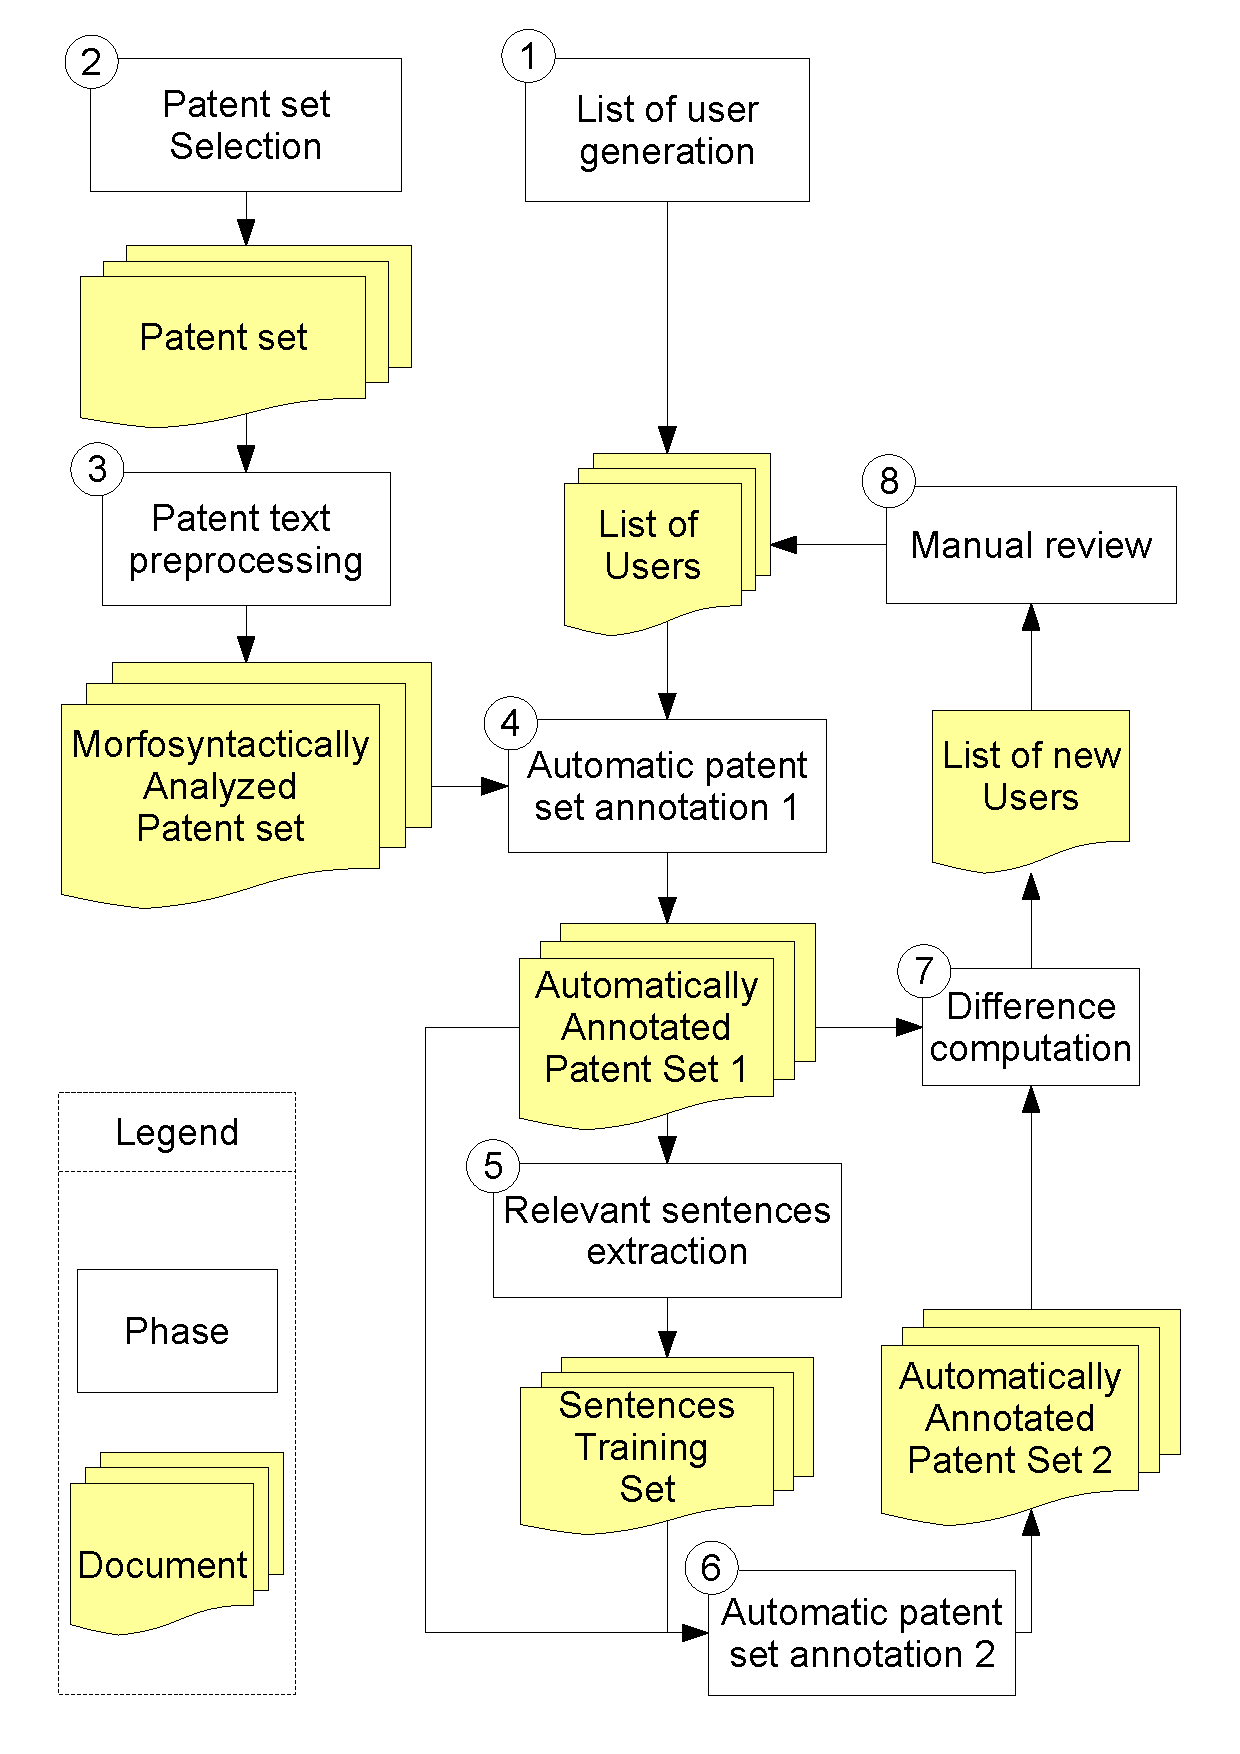
\includegraphics[width=0.6\linewidth]{_bookdown_files/figures/Process} 

}

\caption{Process flow diagram of the proposed automatic user extraction system from patents. The diagram contains the representation of the documents and the operations performed on them. The process takes in input a patent set and a list of users and produces a list of new users as output.}\label{fig:procesuser}
\end{figure}

\subsubsection*{List of users
generation}\label{list-of-users-generation}
\addcontentsline{toc}{subsubsection}{List of users generation}

To generate the input list of users, we used two different approaches: a
bottom-up approach and a top-down approach. The bottom-up approach is
based on the merge of lists from heterogeneous sources. In the present
work we used the following lists of entities:

\begin{itemize}
\item
  \emph{Lists of jobs} :\citep{listjobs}, 11.142 entities
\item
  \emph{Lists of sports and hobbies}\footnote{\url{http://www.notsoboringlife.com/list-of-hobbies/,http://www.notsoboringlife.com/list-of-hobbies/}}:
  9.660 entities;
\end{itemize}

\emph{List of animals} \footnote{\url{http://a-z-animals.com/animals/}}:
600 entities;

\begin{itemize}
\item
  \emph{Lists of patients} \footnote{\url{http://www.medicinenet.com/diseases/_and/_conditions/alpha/_a.htm},
    \url{http://www.cdc.gov/DiseasesConditions/az/a.html}}: 14.609
  users;
\item
  \emph{List of generic words}: manually generated. It contains users
  with a higher level of abstraction (such as \emph{person} or
  \emph{human being}), 56 items.
\end{itemize}

Bottom-up approach produced a list of 35.767 entries.

Afterwards, a top-down approach was applied. Starting from the list
generated with the bottom-up approach, we looked for alternative methods
to indicate a user, finding defined word patterns. The most relevant
are:

\begin{itemize}
\tightlist
\item
  Patterns like ``hobby\_term + practitioner'' for the hobbies;
\item
  Patterns like ``person who has + disease\_term'' or ``suffering from +
  disease\_term'' for the diseases;
\item
  Patterns like ``practitioner of + sport\_term'' for sports.
\end{itemize}

Top-down approach generated a total of 41.090 entries.

The whole process generated a total of 76.857 users and gave us a
reasonable number of terms to be used in the next step of the process.

Obviously our lists have a limited coverage and, therefore, they do not
contain all variations of a certain user. For instance, the lists miss
some users belonging to the classes mentioned above (e.g.~new jobs
emerged in the last years) and all the alternative ways for referring to
a user we do not spotted in the top-down approach. For example our lists
miss jobs like \emph{data analyst}, \emph{lap dancer},
\emph{undertaker}, \emph{mortician} and \emph{thief} or patients with
emerging diseases like \emph{work-alcoholic} and \emph{web-addicted}. In
addition, our lists miss a class of users related to religious groups,
containing users like \emph{christians} or \emph{jewish}. Such terms
have intentionally \textbf{not} been introduced in the input list
because we considered these terms as candidates to be extracted by the
process in our case study .

\subsubsection{Patent set selection \{-\}}\label{patsetsel}

Our choice of patent sets aimed at challenging our system to find new
users missing in the input list. To reproduce a patent set selection, we
took into consideration the International Patent Classification (IPC)
\citep{wipo1}. IPC is a hierarchical system of patent classes
representing different areas of technology. Then, we wondered which
classes could contain new users according to our seed list. Furthermore,
IPC class A, which is the first level in IPC differentiation, is based
on human necessities. For this reason, we assumed that in this class we
would have found likely users from patents texts.

\subsubsection*{Patent text analysis}\label{patent-text-analysis}
\addcontentsline{toc}{subsubsection}{Patent text analysis}

Our Entity Extraction system is composed by a set of sequential phases.
The first three phases are related to the linguistic annotation:
sentence splitting and tokenization, part of speech tagging and
lemmatization. Then, the patent set is analyzed by the entity extractor,
specialized for users extraction. A more detailed description of each
phase is:

\begin{itemize}
\item
  Sentence splitting and Tokenization: These processes split the text
  into sentences and then segment each sentence in orthographic units
  called tokens. In our system, sentence splitting plays a key role
  since thanks to a given word, it is possible to find sentences where
  the word is used. Finding correct boundaries for a specific word
  allows to dramatically reduce the space to retrieve its surrounding
  contexts.
\item
  POS tagging and Lemmatization: The Part-Of-Speech tagging (or POS
  tagging) is the process of assigning unambiguous grammatical
  categories to words in context. It plays a key role in NLP and in many
  language technology systems. For the present application we used the
  most recent version of the Felice-POS-tagger described in
  \citep{dell2009ensemble}. Once the computation of the POS-tagged text
  is completed, the text is lemmatized according to the result of this
  analysis.
\item
  Semi-automatic Users Annotation: The Users Extraction tool is based on
  supervised methods. Such methods require an entity annotated corpus in
  order to extract new entities from unseen documents. A semi-automatic
  method has been used to generate an annotated corpus of users to avoid
  manual annotation of a patent set. The method is a projection of the
  list of users on the patent set. The list of users is cleaned to avoid
  linguistic ambiguities when projecting these entities on the corpus.
  For example, the term \emph{``guide''} has two different meanings when
  used as a verb or as a noun. Furthermore, as a noun it could indicate
  a component of a system (guide for mechanical parts) or a person
  (someone employed to conduct others) and therefore a user. Avoiding
  ambiguities is a crucial aspect to produce an informative training
  set, so ambiguous words were pruned.
\end{itemize}

The entity annotation schema for a single token is defined using a
widely accepted BIO annotation scheme \cite{ramshaw}:

\begin{itemize}
\tightlist
\item
  \textbf{B-USE}: the token is the beginning of an entity representing
  an User;
\item
  \textbf{I-USE}: the token is the continuation of a sequence of tokens
  representing an User;
\item
  \textbf{O}: for all the other cases.
\end{itemize}

\subsubsection*{User Entity Extraction}\label{user-entity-extraction}
\addcontentsline{toc}{subsubsection}{User Entity Extraction}

The Users extraction problem is tackled by the implementation of a
supervised classifier that is trained on an annotated patent set. Thus,
the patent set is linguistically-annotated, using the steps described
above and entity-annotated, exploiting the semiautomatic annotation
process executed in the previous steps.

Given a set of features the classifier trains a statistical model using
the feature statistics extracted from the corpus. For each new document
the trained model assigns to each word the probability of belonging to
one of the classes previously defined (B-USE, I-USE, O).

In our experiments the classifier has been trained using two different
learning algorithms: Support Vector Machines (SVM) using the LIBSVM
library \citep{svm} configured to use a linear kernel and Multi Layer
Perceptron (MLP) implemented using the Keras library \citep{libkeras}.
It has been proven that Long Short Term Memory Recurrent Neural Network
(LSTM) \citep{chiu2016named} methods are well suited for similar NER
task. Anyway, we chose SVM and MLP method to study how two wheel
established state of the art classifiers perform on the specific task of
user extraction from patents and to evaluate their performance in terms
of precision and computational effort. We also think that the popularity
of these methods increment the reproducibility of the work.

The classifier uses different kind of features extracted from the text:

\begin{itemize}
\item
  \emph{linguistic features}, i.e.~lemma, Part-Of-Speech, prefix and
  suffix of the analyzed token;
\item
  \emph{contextual features}, the linguistic characteristics of the
  context words of the analyzed token; in addition the entity category
  of the previous token is considered;
\item
  \emph{compositional features}, combinations of contextual features and
  linguistic features. i.e.~Part-Of-Speech of the previous word and the
  lemma of the current word. These extra features allow to infer
  statistics on the interaction of the combined features that can not be
  captured by a linear SVM model.
\item
  \emph{word2vec features}: vector representations of words computed by
  the \emph{word2vec} \citep{word2vec1} tool.
\end{itemize}

\emph{Word2vec} is a NLP tool able to produce word representations
exploiting big corpora. The main property of the vectors produced by
\emph{word2vec} is that words sharing similar contexts have similar
vector representations. By using word vectors instead of the
corresponding words we were able overcome the problem of the limited
lexical knowledge in the training phase. Using these features and
excluding all the others (delexicalized model) we expected that the
resulting user extraction system had a lower precision and an higher
recall in the classification phase. We presumed to find new users not
contained in the input seed list.

\subsubsection*{Manual Review of the new list of
users}\label{manual-review-of-the-new-list-of-users}
\addcontentsline{toc}{subsubsection}{Manual Review of the new list of
users}

It is still possible that the classification process creates false
positive results (words labeled as users that do not match the
definition in section @ref\{usersresults\}). Thus, it is necessary to
make a manual review of the extracted entities with the aim of
evaluating the output.

\subsection{Results}\label{results}

The following section describes the performances of the automatic users
extraction process on two different patent sets. To test the system four
experiments were conducted\}. Finally the performances and the outcomes
of the system are shown and discussed.

Following the guidelines for the patent set selection @ref\{patsetsel\},
we examined two patent sets belonging to the IPC class A:

\begin{itemize}
\tightlist
\item
  \textbf{A47G33}. The IPC definition of the subclass is
  \emph{``religious or ritual equipment in dwelling or for general''}.
\item
  \textbf{A61G1-A61G13}. The IPC definition of the subclass A61G1 is
  \emph{``Stretchers''} while the definition of the subclass A61G13 is
  \emph{``Operating tables; Auxiliary appliances therefor''}.
\end{itemize}

We extracted from the private Errequadro s.r.l. \footnote{\url{http://www.errequadrosrl.com/}}
database a random sample of 2.000 patents from each IPC class. We have
chosen this database because of the reliability of the data given by
this copany with respect to the public available databases. Furthermore
it is not always possibile to have acces to the full text of a patent
for free. For each patent set we applied the semiautomatic set
annotation process by projecting the input list of users on the
morphosyntactically analyzed patent set. After this process, each
semi-automatically annotated patent set was split in two parts: the
first was used as training set for the user extractor, and the second
one was used as test set.

To build an informative training set, from the semi-automatically patent
set we selected a subset of sentences containing at least one user. The
size of the training set in both cases is approximately composed by
600.000 tokens. For each patent set table \ref{tab:patentsetdetails}
shows the number of sentences of the training set, the number of
sentences of the test set, and the number of distinct users in the
training set (re-projected by the semi-automatic annotation process).

\begin{longtable}[]{@{}cccc@{}}
\caption{\label{tab:patentsetdetails} Statistics related to the patent set
groups analyzed in the case study}\tabularnewline
\toprule
\begin{minipage}[b]{0.16\columnwidth}\centering\strut
\emph{patent set group}\strut
\end{minipage} & \begin{minipage}[b]{0.21\columnwidth}\centering\strut
\emph{\#Sentences - training}\strut
\end{minipage} & \begin{minipage}[b]{0.18\columnwidth}\centering\strut
\emph{\#Sentences - test}\strut
\end{minipage} & \begin{minipage}[b]{0.33\columnwidth}\centering\strut
\emph{\#Distinct users projected on training}\strut
\end{minipage}\tabularnewline
\midrule
\endfirsthead
\toprule
\begin{minipage}[b]{0.16\columnwidth}\centering\strut
\emph{patent set group}\strut
\end{minipage} & \begin{minipage}[b]{0.21\columnwidth}\centering\strut
\emph{\#Sentences - training}\strut
\end{minipage} & \begin{minipage}[b]{0.18\columnwidth}\centering\strut
\emph{\#Sentences - test}\strut
\end{minipage} & \begin{minipage}[b]{0.33\columnwidth}\centering\strut
\emph{\#Distinct users projected on training}\strut
\end{minipage}\tabularnewline
\midrule
\endhead
\begin{minipage}[t]{0.16\columnwidth}\centering\strut
A47G33\strut
\end{minipage} & \begin{minipage}[t]{0.21\columnwidth}\centering\strut
13.364\strut
\end{minipage} & \begin{minipage}[t]{0.18\columnwidth}\centering\strut
214.029\strut
\end{minipage} & \begin{minipage}[t]{0.33\columnwidth}\centering\strut
126\strut
\end{minipage}\tabularnewline
\begin{minipage}[t]{0.16\columnwidth}\centering\strut
A61G1-A61G13\strut
\end{minipage} & \begin{minipage}[t]{0.21\columnwidth}\centering\strut
15.108\strut
\end{minipage} & \begin{minipage}[t]{0.18\columnwidth}\centering\strut
2.520.350\strut
\end{minipage} & \begin{minipage}[t]{0.33\columnwidth}\centering\strut
121\strut
\end{minipage}\tabularnewline
\bottomrule
\end{longtable}

We chose two orders of magnitude for the sentences test-set to test the
efficiency of multiple configurations of the system.

To test the performances of the implemented user extractor, we devised
four different configurations. Each configuration uses a specific
learning algorithm and a set of features to build the statistical model.
The main purpose of this procedure is to find the configurations that
better perform in the user extraction task. In addition, the different
behaviour of the system in the classification phase is studied. In table
\ref{tab:feat-confs} are reported the detailed configurations used in
our experiments.

\begin{longtable}[]{@{}cc@{}}
\caption{\label{tab:feat-confs} Context windows of the extracted features
considering 0 as the current analyzed token.}\tabularnewline
\toprule
\emph{Feature group} & \emph{Context Window}\tabularnewline
\midrule
\endfirsthead
\toprule
\emph{Feature group} & \emph{Context Window}\tabularnewline
\midrule
\endhead
Lemma unigrams & \textbackslash{}({[}-2, -1, 0,
1{]}\textbackslash{})\tabularnewline
Lemma bigrams & \textbackslash{}({[}(-1 ,0), (0,
1){]}\textbackslash{})\tabularnewline
Word bigrams & \textbackslash{}({[}(-1 ,0), (-2, -1), (0, 1), (1,
2){]}\textbackslash{})\tabularnewline
Word trigrams & \textbackslash{}({[}(1, 0, 1) (-2, 1,
0){]}\textbackslash{})\tabularnewline
Pos unigrams & \textbackslash{}({[}-2, -1, 0,
1{]}\textbackslash{})\tabularnewline
Pos bigrams & \textbackslash{}(({[}(-2, -1) (-1, 0),
(0,1){]})\textbackslash{})\tabularnewline
Compositional feature \#1 & \textbackslash{}((POS\_\{-1\},
Lemma\_\{0\})\textbackslash{})\tabularnewline
Compositional feature \#2 & \textbackslash{}((Lemma\_\{-1\},
Lemma\_\{0\})\textbackslash{})\tabularnewline
Compositional feature \#3 & \textbackslash{}((Lemma\_\{0\},
Lemma\_\{1\})\textbackslash{})\tabularnewline
Compositional feature \#4 & \textbackslash{}((POS\_\{0\},
Lemma\_\{1\})\textbackslash{})\tabularnewline
Compositional feature \#5 & \textbackslash{}((NER\_\{-1\},
Lemma\_\{0\})\textbackslash{})\tabularnewline
Word2vec & \(-2, -1, 0, 1, 2\)\tabularnewline
\bottomrule
\end{longtable}

By using the first and the second configuration we expected to have a
higher precision in the classification phase, since explicit lexical
information is used in the training phase. For the same reason we
expected to have low recall in classification phase. On the other hand,
the third and fourth configurations are delexicalized: lexical
information is provided by word vectors computed by word2vec. In these
two configurations we expected to have an higher recall and a lower
precision, due to the characteristics of the computed vectors explained
before. To limit errors when using the \emph{word2vec} features, some
linguistically motivated filtering rules were introduced. Specifically,
sequences of tokens classified as users were constrained from the
following categories: verbs, adjectives not preceded by articles,
articles and adverbs.

To evaluate the whole user extraction process in each experiment, we
defined some evaluation measures. Each measure was introduced to
evaluate the characteristics of the extraction system concerning the
configuration applied.

These measures are:

\begin{itemize}
\tightlist
\item
  Training time: time needed to create the statistical model using the
  training set;
\item
  Test time: time needed to re-annotate the semi-automatically annotated
  patent set;
\item
  Number of extracted users: number of unique entities classified as
  user in the automatically annotated patent set;
\item
  Number of known users: number of distinct extracted users in the
  automatically annotated patent set and belonging to the list of user
  in input;
\item
  Number of new users: number of distinct entities classified as user in
  the automatically annotated patent set and not belonging to the input
  list of users;
\item
  Number of new correct users: number of distinct entities considered as
  user and as correct after a manual review;
\item
  Precision: ratio between the number of new distinct correct users and
  the total number of new distinct users;
\item
  Gain: ratio between the number of new distinct correct users and the
  number of re-projected distinct users on the training set.
\end{itemize}

Table \ref{tab:runs-data} reports the values of the defined metrics
across all the experiments run on the two patent sets.

\begin{longtable}[]{@{}lccccccccc@{}}
\caption{\label{tab:runs-data} Comparison of the values of the defined
metrics across all the experiments. The patent set annotation in the
experiment (6) was not performed due to the computational costs. All the
experiments were run on a machine provided with 10 AMD Opteron(tm) 6376
processors.}\tabularnewline
\toprule
\begin{minipage}[b]{0.09\columnwidth}\raggedright\strut
Experiment\strut
\end{minipage} & \begin{minipage}[b]{0.10\columnwidth}\centering\strut
Training time\strut
\end{minipage} & \begin{minipage}[b]{0.08\columnwidth}\centering\strut
Test Time\strut
\end{minipage} & \begin{minipage}[b]{0.08\columnwidth}\centering\strut
Extracted\strut
\end{minipage} & \begin{minipage}[b]{0.05\columnwidth}\centering\strut
Known\strut
\end{minipage} & \begin{minipage}[b]{0.04\columnwidth}\centering\strut
New\strut
\end{minipage} & \begin{minipage}[b]{0.09\columnwidth}\centering\strut
New correct\strut
\end{minipage} & \begin{minipage}[b]{0.08\columnwidth}\centering\strut
New wrong\strut
\end{minipage} & \begin{minipage}[b]{0.08\columnwidth}\centering\strut
Prec. (\%)\strut
\end{minipage} & \begin{minipage}[b]{0.07\columnwidth}\centering\strut
Gain (\%)\strut
\end{minipage}\tabularnewline
\midrule
\endfirsthead
\toprule
\begin{minipage}[b]{0.09\columnwidth}\raggedright\strut
Experiment\strut
\end{minipage} & \begin{minipage}[b]{0.10\columnwidth}\centering\strut
Training time\strut
\end{minipage} & \begin{minipage}[b]{0.08\columnwidth}\centering\strut
Test Time\strut
\end{minipage} & \begin{minipage}[b]{0.08\columnwidth}\centering\strut
Extracted\strut
\end{minipage} & \begin{minipage}[b]{0.05\columnwidth}\centering\strut
Known\strut
\end{minipage} & \begin{minipage}[b]{0.04\columnwidth}\centering\strut
New\strut
\end{minipage} & \begin{minipage}[b]{0.09\columnwidth}\centering\strut
New correct\strut
\end{minipage} & \begin{minipage}[b]{0.08\columnwidth}\centering\strut
New wrong\strut
\end{minipage} & \begin{minipage}[b]{0.08\columnwidth}\centering\strut
Prec. (\%)\strut
\end{minipage} & \begin{minipage}[b]{0.07\columnwidth}\centering\strut
Gain (\%)\strut
\end{minipage}\tabularnewline
\midrule
\endhead
\begin{minipage}[t]{0.09\columnwidth}\raggedright\strut
\strut
\end{minipage} & \begin{minipage}[t]{0.10\columnwidth}\centering\strut
\strut
\end{minipage} & \begin{minipage}[t]{0.08\columnwidth}\centering\strut
\strut
\end{minipage} & \begin{minipage}[t]{0.08\columnwidth}\centering\strut
\strut
\end{minipage} & \begin{minipage}[t]{0.05\columnwidth}\centering\strut
\strut
\end{minipage} & \begin{minipage}[t]{0.04\columnwidth}\centering\strut
\strut
\end{minipage} & \begin{minipage}[t]{0.09\columnwidth}\centering\strut
\strut
\end{minipage} & \begin{minipage}[t]{0.08\columnwidth}\centering\strut
\strut
\end{minipage} & \begin{minipage}[t]{0.08\columnwidth}\centering\strut
\strut
\end{minipage} & \begin{minipage}[t]{0.07\columnwidth}\centering\strut
\strut
\end{minipage}\tabularnewline
\begin{minipage}[t]{0.09\columnwidth}\raggedright\strut
1 (SVM)\strut
\end{minipage} & \begin{minipage}[t]{0.10\columnwidth}\centering\strut
83m\strut
\end{minipage} & \begin{minipage}[t]{0.08\columnwidth}\centering\strut
321m\strut
\end{minipage} & \begin{minipage}[t]{0.08\columnwidth}\centering\strut
161\strut
\end{minipage} & \begin{minipage}[t]{0.05\columnwidth}\centering\strut
93\strut
\end{minipage} & \begin{minipage}[t]{0.04\columnwidth}\centering\strut
68\strut
\end{minipage} & \begin{minipage}[t]{0.09\columnwidth}\centering\strut
47\strut
\end{minipage} & \begin{minipage}[t]{0.08\columnwidth}\centering\strut
21\strut
\end{minipage} & \begin{minipage}[t]{0.08\columnwidth}\centering\strut
69.11\strut
\end{minipage} & \begin{minipage}[t]{0.07\columnwidth}\centering\strut
37.30\strut
\end{minipage}\tabularnewline
\begin{minipage}[t]{0.09\columnwidth}\raggedright\strut
2 (MLP)\strut
\end{minipage} & \begin{minipage}[t]{0.10\columnwidth}\centering\strut
1911m\strut
\end{minipage} & \begin{minipage}[t]{0.08\columnwidth}\centering\strut
9091m\strut
\end{minipage} & \begin{minipage}[t]{0.08\columnwidth}\centering\strut
196\strut
\end{minipage} & \begin{minipage}[t]{0.05\columnwidth}\centering\strut
55\strut
\end{minipage} & \begin{minipage}[t]{0.04\columnwidth}\centering\strut
141\strut
\end{minipage} & \begin{minipage}[t]{0.09\columnwidth}\centering\strut
27\strut
\end{minipage} & \begin{minipage}[t]{0.08\columnwidth}\centering\strut
114\strut
\end{minipage} & \begin{minipage}[t]{0.08\columnwidth}\centering\strut
19.15\strut
\end{minipage} & \begin{minipage}[t]{0.07\columnwidth}\centering\strut
21.42\strut
\end{minipage}\tabularnewline
\begin{minipage}[t]{0.09\columnwidth}\raggedright\strut
3 (MLP-W2V)\strut
\end{minipage} & \begin{minipage}[t]{0.10\columnwidth}\centering\strut
165m\strut
\end{minipage} & \begin{minipage}[t]{0.08\columnwidth}\centering\strut
246m\strut
\end{minipage} & \begin{minipage}[t]{0.08\columnwidth}\centering\strut
162\strut
\end{minipage} & \begin{minipage}[t]{0.05\columnwidth}\centering\strut
35\strut
\end{minipage} & \begin{minipage}[t]{0.04\columnwidth}\centering\strut
127\strut
\end{minipage} & \begin{minipage}[t]{0.09\columnwidth}\centering\strut
45\strut
\end{minipage} & \begin{minipage}[t]{0.08\columnwidth}\centering\strut
82\strut
\end{minipage} & \begin{minipage}[t]{0.08\columnwidth}\centering\strut
35.43\strut
\end{minipage} & \begin{minipage}[t]{0.07\columnwidth}\centering\strut
35.71\strut
\end{minipage}\tabularnewline
\begin{minipage}[t]{0.09\columnwidth}\raggedright\strut
4 (SVM-W2V)\strut
\end{minipage} & \begin{minipage}[t]{0.10\columnwidth}\centering\strut
1265m\strut
\end{minipage} & \begin{minipage}[t]{0.08\columnwidth}\centering\strut
4310m\strut
\end{minipage} & \begin{minipage}[t]{0.08\columnwidth}\centering\strut
121\strut
\end{minipage} & \begin{minipage}[t]{0.05\columnwidth}\centering\strut
29\strut
\end{minipage} & \begin{minipage}[t]{0.04\columnwidth}\centering\strut
92\strut
\end{minipage} & \begin{minipage}[t]{0.09\columnwidth}\centering\strut
45\strut
\end{minipage} & \begin{minipage}[t]{0.08\columnwidth}\centering\strut
47\strut
\end{minipage} & \begin{minipage}[t]{0.08\columnwidth}\centering\strut
48.91\strut
\end{minipage} & \begin{minipage}[t]{0.07\columnwidth}\centering\strut
35.71\strut
\end{minipage}\tabularnewline
\begin{minipage}[t]{0.09\columnwidth}\raggedright\strut
\strut
\end{minipage} & \begin{minipage}[t]{0.10\columnwidth}\centering\strut
\strut
\end{minipage} & \begin{minipage}[t]{0.08\columnwidth}\centering\strut
\strut
\end{minipage} & \begin{minipage}[t]{0.08\columnwidth}\centering\strut
\strut
\end{minipage} & \begin{minipage}[t]{0.05\columnwidth}\centering\strut
\strut
\end{minipage} & \begin{minipage}[t]{0.04\columnwidth}\centering\strut
\strut
\end{minipage} & \begin{minipage}[t]{0.09\columnwidth}\centering\strut
\strut
\end{minipage} & \begin{minipage}[t]{0.08\columnwidth}\centering\strut
\strut
\end{minipage} & \begin{minipage}[t]{0.08\columnwidth}\centering\strut
\strut
\end{minipage} & \begin{minipage}[t]{0.07\columnwidth}\centering\strut
\strut
\end{minipage}\tabularnewline
\begin{minipage}[t]{0.09\columnwidth}\raggedright\strut
5 (SVM)\strut
\end{minipage} & \begin{minipage}[t]{0.10\columnwidth}\centering\strut
148m\strut
\end{minipage} & \begin{minipage}[t]{0.08\columnwidth}\centering\strut
3443m\strut
\end{minipage} & \begin{minipage}[t]{0.08\columnwidth}\centering\strut
302\strut
\end{minipage} & \begin{minipage}[t]{0.05\columnwidth}\centering\strut
120\strut
\end{minipage} & \begin{minipage}[t]{0.04\columnwidth}\centering\strut
182\strut
\end{minipage} & \begin{minipage}[t]{0.09\columnwidth}\centering\strut
88\strut
\end{minipage} & \begin{minipage}[t]{0.08\columnwidth}\centering\strut
108\strut
\end{minipage} & \begin{minipage}[t]{0.08\columnwidth}\centering\strut
48.35\strut
\end{minipage} & \begin{minipage}[t]{0.07\columnwidth}\centering\strut
72.72\strut
\end{minipage}\tabularnewline
\begin{minipage}[t]{0.09\columnwidth}\raggedright\strut
6 (MLP)\strut
\end{minipage} & \begin{minipage}[t]{0.10\columnwidth}\centering\strut
1818m\strut
\end{minipage} & \begin{minipage}[t]{0.08\columnwidth}\centering\strut
---\strut
\end{minipage} & \begin{minipage}[t]{0.08\columnwidth}\centering\strut
---\strut
\end{minipage} & \begin{minipage}[t]{0.05\columnwidth}\centering\strut
---\strut
\end{minipage} & \begin{minipage}[t]{0.04\columnwidth}\centering\strut
---\strut
\end{minipage} & \begin{minipage}[t]{0.09\columnwidth}\centering\strut
---\strut
\end{minipage} & \begin{minipage}[t]{0.08\columnwidth}\centering\strut
---\strut
\end{minipage} & \begin{minipage}[t]{0.08\columnwidth}\centering\strut
---\strut
\end{minipage} & \begin{minipage}[t]{0.07\columnwidth}\centering\strut
---\strut
\end{minipage}\tabularnewline
\begin{minipage}[t]{0.09\columnwidth}\raggedright\strut
7 (MLP-W2V)\strut
\end{minipage} & \begin{minipage}[t]{0.10\columnwidth}\centering\strut
333m\strut
\end{minipage} & \begin{minipage}[t]{0.08\columnwidth}\centering\strut
3530m\strut
\end{minipage} & \begin{minipage}[t]{0.08\columnwidth}\centering\strut
305\strut
\end{minipage} & \begin{minipage}[t]{0.05\columnwidth}\centering\strut
38\strut
\end{minipage} & \begin{minipage}[t]{0.04\columnwidth}\centering\strut
267\strut
\end{minipage} & \begin{minipage}[t]{0.09\columnwidth}\centering\strut
44\strut
\end{minipage} & \begin{minipage}[t]{0.08\columnwidth}\centering\strut
230\strut
\end{minipage} & \begin{minipage}[t]{0.08\columnwidth}\centering\strut
16.48\strut
\end{minipage} & \begin{minipage}[t]{0.07\columnwidth}\centering\strut
36.36\strut
\end{minipage}\tabularnewline
\begin{minipage}[t]{0.09\columnwidth}\raggedright\strut
8 (SVM-W2V)\strut
\end{minipage} & \begin{minipage}[t]{0.10\columnwidth}\centering\strut
1268m\strut
\end{minipage} & \begin{minipage}[t]{0.08\columnwidth}\centering\strut
47020m\strut
\end{minipage} & \begin{minipage}[t]{0.08\columnwidth}\centering\strut
313\strut
\end{minipage} & \begin{minipage}[t]{0.05\columnwidth}\centering\strut
49\strut
\end{minipage} & \begin{minipage}[t]{0.04\columnwidth}\centering\strut
264\strut
\end{minipage} & \begin{minipage}[t]{0.09\columnwidth}\centering\strut
74\strut
\end{minipage} & \begin{minipage}[t]{0.08\columnwidth}\centering\strut
197\strut
\end{minipage} & \begin{minipage}[t]{0.08\columnwidth}\centering\strut
28.03\strut
\end{minipage} & \begin{minipage}[t]{0.07\columnwidth}\centering\strut
61.15\strut
\end{minipage}\tabularnewline
\bottomrule
\end{longtable}

For what concerns training and test time of the automatic patent set
annotation, it's clear that the configuration based on the SVM learning
algorithm without the \emph{word2vec} features performs better in both
the experiments (1, 5). When the features based on \emph{word2vec} are
introduced, the configuration based on the MLP learning algorithm is the
fastest both in training and test time (3, 6): it is due to the fact
that keras implementation of this algorithm exploits all the available
CPU cores of the system. On the other side, the MLP algorithm does not
scale properly with a higher number of features, as seen in training and
annotation time in the experiment (2). In addition, we could not perform
the patent set annotation in the experiment (6), since it would have
required more than 60 machine days to complete the process. When
\emph{word2vec} features are introduced, the patent set annotation based
on the SVM algorithm is 10 times slower than the MLP algorithm.

For what concerns the precision in the automatic patent set annotation,
the SVM configuration without \emph{word2vec} features is clearly the
more reliable: the precision values are from 1.5 to 2 times higher in
the experiments (1, 5) in contrast to the other experiments. The higher
precision is justified by the fact that the configurations based on
\emph{word2vec} features lack explicit lexical information: words with
very similar contexts are represented by similar \emph{word2vec}
vectors, probably leading to errors in the classification phase. On the
other hand, the use of \emph{word2vec} vectors aims at extracting
entities that would not be extracted by considering explicit lexical
information only.

Finally, for what concerns information gain, the same amount of new
information (21-37\%) is extracted in the experiments on the A47G33
patent set. The gain values drastically change in the experiments on the
A61G1-A61G13 patent set: in the experiments (5, 8) a gain between 61\%
and 72\% is obtained: it is due to the size of this patent set in
comparison to the A47G33 one. In the experiment (7), despite the
introduction of \emph{word2vec} features, a gain of 36\% is obtained.
This fact, in conjunction with the non-feasibility of the experimental
configuration 6, shows how MLP systems lack in efficacy and efficiency
(in entity extraction in patent domain) when the test-set has an order
of magnitude of millions of sentences. We think that this result is
relevant, based on our experience with practical applications.

Furthremore, a way to maximize the overall informative gain is to merge
the results of all manually reviewed user extractions obtained by
executing the patent set annotation process with all possible
configurations.

The overall informative gain of the merging process is related to
intersections that occur among the results obtained by the patent set
annotation process in each configuration: the less the intersections,
the more the overall informative gain obtained. In table
\ref{tab:mergedata} is shown the overall gain obtained by merging
results of the manually reviewed extractions in each patent set.

\begin{longtable}[]{@{}ccc@{}}
\caption{\label{tab:mergedata} Gain obtained by merging correct entities
extracted from each patent set annotation.}\tabularnewline
\toprule
Configuration & A47G33 - Gain (\%) & A61G1+A61G11 - Gain
(\%)\tabularnewline
\midrule
\endfirsthead
\toprule
Configuration & A47G33 - Gain (\%) & A61G1+A61G11 - Gain
(\%)\tabularnewline
\midrule
\endhead
SVM & 37.30 & 72.72\tabularnewline
MLP & 21.42 & ---\tabularnewline
MLP-W2V & 35.71 & 36.36\tabularnewline
SVM-W2V & 35.71 & 61.15\tabularnewline
SVM - MLP & 52.38 & ---\tabularnewline
SVM - MLP-W2V & 69.84 & 126.44\tabularnewline
SVM - SVM-W2V & 73.01 & 103.30\tabularnewline
MLP - MLP-W2V & 55.55 & ---\tabularnewline
MLP - SVM-W2V & 57.14 & ---\tabularnewline
MLP-W2V - SVM-W2V & 59.52 & 76.30\tabularnewline
SVM - SVM-W2V - MLP-W2V & 90.47 & 140.49\tabularnewline
SVM - MLP - MLP-W2V & 82.53 & ---\tabularnewline
SVM - MLP - SVM-W2V & 85.71 & ---\tabularnewline
MLP - SVM-W2V - MLP-W2V & 77.77 & ---\tabularnewline
SVM - MLP - SVM-W2V - MLP-W2V & 103.17 & ---\tabularnewline
\bottomrule
\end{longtable}

The table shows that the merging process of manually reviewed entities
extracted from each patent set annotation run effectively contributes to
increase the overall informative gain. For instance in the A47G33 patent
set an overall gain of 103.17\% is obtained, tripling the best result
achieved by the extraction performed using the best single
configuration. Good results are also achieved in the A47G33 patent set
user extraction. In this case an overall gain of 140.49\% is obtained,
doubling the best result achieved by the extraction performed using the
best single configuration.

The results shown in section 5 prove that if the goal of the extraction
is to reach the maximal recall, an ensemble method (combining the output
of multiple classifier) over-performs every single classifier method.
Anyway, the ensemble approach has clear efficiency issues, because the
time of analysis will be the sum of every single approach time (in
hypotheses of non-parallelization). This leads to a trade off between
the speed of the system and the quality of the results, and whoever
would use the presented system can decide to gain benefit in one or in
another direction.

Finally, tables \ref{tab:result-extraction-dl-a47g33} and
\ref{tab:result-extraction-dlw2v-a47g33} show an overview of extracted
users randomly chosen from the A47G33 patent set (the only one in which
were able to perform all experiments). Each table is divided in two
blocks, representing the results of the extraction performed using a
specific configuration. For each extracted user is shown the
corresponding lemma (the root form), the frequency (how many times that
user appears in the whole corpus) and the total number of patents
containing the user. Users not contained in the starting user list, are
highlighted in bold.

The table shows that the system was able to extract characteristic users
of the patent set. The results are in fact not unexpected for the IPC
class under analysis: this is an evidence of the correct performances of
the proposed system. In other words, the results presented in the table
show that it is possible to train a NER systems able to extract sparse
and valuable information. Such users are the ones that an expert would
manually extract but the NER system does it with an enormous saving in
terms of time and efforts.

Other remarkable results are:

\begin{itemize}
\item
  many newly extracted entities have very low frequency in the patent
  set: it shows that the developed system is able to extract rare
  entities.
\item
  table \ref{tab:result-extraction-dlw2v-a47g33} shows that
  configurations using \emph{word2vec} features are able to find new
  users with a higher frequency in the patent set: it was an expected
  result, since the \emph{word2vec} configurations are not explicitly
  lexicalized and more able to generalize during extraction phase.
\item
  The system is able to extract single words and multi-words.
\item
  Taking into consideration the definition of user of an invention, the
  system extracts unusual and sometimes borderline users. Examples like
  \emph{saint}, \emph{angel}, \emph{god} and \emph{ghost} need
  discussion that is far beyond the purposes of the present thesis.
  These results are a remarkable evidence of the human-like
  generalization ability of the described method.
\end{itemize}

\begin{longtable}[]{@{}cccccc@{}}
\caption{\label{tab:result-extraction-dl-a47g33} Extracted users from the
A47G33 patent set using the SVM and DL configurations. New users
extracted by the system are reported in bold.}\tabularnewline
\toprule
Lemma & Frequency & \# Patents & Lemma & Frequency & \#
Patents\tabularnewline
female & 801 & 109 & child & 402 & 102\tabularnewline
child & 426 & 108 & cleregy member & 128 & 5\tabularnewline
guy & 156 & 17 & patient & 113 & 11\tabularnewline
patient & 115 & 11 & man & 50 & 26\tabularnewline
parent & 70 & 31 & young & 48 & 32\tabularnewline
man & 51 & 26 & \textbf{angel} & 29 & 23\tabularnewline
merchant & 50 & 6 & dog & 20 & 7\tabularnewline
soon & 46 & 29 & artisan & 12 & 12\tabularnewline
engineer & 45 & 45 & \textbf{male/female} & 12 & 4\tabularnewline
adult & 39 & 23 & hockey player & 7 & 1\tabularnewline
young & 35 & 24 & \textbf{professional} & 7 & 7\tabularnewline
society & 32 & 21 & tennis player & 7 & 4\tabularnewline
\textbf{angel} & 29 & 23 & football player & 6 & 3\tabularnewline
fund raiser & 27 & 4 & \textbf{ghost} & 5 & 3\tabularnewline
priest & 22 & 4 & children & 5 & 5\tabularnewline
cheerleader & 15 & 4 & manager & 5 & 5\tabularnewline
\textbf{fund-raiser} & 11 & 4 & \textbf{spider} & 5 & 5\tabularnewline
\textbf{athlete} & 10 & 9 & \textbf{vandal} & 5 & 1\tabularnewline
\textbf{ghost} & 5 & 5 & \textbf{athlete} & 4 & 3\tabularnewline
\textbf{adulterant} & 3 & 3 & mother & 4 & 2\tabularnewline
\textbf{jew} & 3 & 3 & soccer player & 4 & 3\tabularnewline
\textbf{maid} & 3 & 1 & squirrel & 3 & 2\tabularnewline
\textbf{tourist} & 3 & 3 & \textbf{maid} & 3 & 1\tabularnewline
\textbf{indian} & 2 & 2 & \textbf{god} & 3 & 2\tabularnewline
\textbf{beginner} & 1 & 1 & \textbf{mariner} & 3 & 3\tabularnewline
\textbf{christians} & 1 & 1 & \textbf{male-female} & 2 &
2\tabularnewline
\textbf{datum entry operator} & 1 & 1 & \textbf{manufacturer} & 2 &
2\tabularnewline
\textbf{expert} & 1 & 1 & \textbf{jew} & 1 & 1\tabularnewline
\textbf{jewish} & 1 & 1 & \textbf{merchandizers} & 1 & 1\tabularnewline
\textbf{marinaro} & 1 & 1 & \textbf{parishioner} & 1 & 1\tabularnewline
\bottomrule
\end{longtable}

\begin{longtable}[]{@{}cccccc@{}}
\caption{\label{tab:result-extraction-dlw2v-a47g33} Extracted users from the
A47G33 patent set using the SVM-W2V and MLP-W2V configurations. New
users extracted by the system are reported in bold.}\tabularnewline
\toprule
Lemma & Frequency & \# Patents & Lemma & Frequency & \#
Patents\tabularnewline
child & 152 & 68 & clergy member & 124 & 5\tabularnewline
clergy member & 124 & 5 & \textbf{crowd} & 36 & 3\tabularnewline
man & 50 & 26 & basketball player & 20 & 5\tabularnewline
engineer & 45 & 45 & \textbf{him} & 17 & 8\tabularnewline
young & 29 & 24 & woman & 16 & 8\tabularnewline
\textbf{choir} & 17 & 1 & \textbf{saint} & 14 & 2\tabularnewline
\textbf{infirm} & 13 & 8 & \textbf{youth} & 14 & 2\tabularnewline
\textbf{bride} & 9 & 4 & \textbf{angel} & 8 & 4\tabularnewline
\textbf{volunteer} & 8 & 6 & \textbf{choir} & 8 & 1\tabularnewline
musician & 6 & 6 & musician & 6 & 6\tabularnewline
boy & 3 & 1 & \textbf{god} & 5 & 1\tabularnewline
children & 3 & 3 & children & 3 & 3\tabularnewline
girl & 3 & 2 & guy & 3 & 3\tabularnewline
\textbf{creature} & 2 & 1 & infant & 3 & 3\tabularnewline
\textbf{deceased} & 2 & 1 & priest & 3 & 3\tabularnewline
\textbf{jewish} & 2 & 2 & \textbf{bride} & 2 & 2\tabularnewline
\textbf{person} & 2 & 2 & \textbf{consumer} & 2 & 2\tabularnewline
mother & 2 & 2 & \textbf{everyone} & 2 & 2\tabularnewline
\textbf{audience} & 1 & 1 & \textbf{him/her} & 2 & 2\tabularnewline
\textbf{boyfriend} & 1 & 1 & \textbf{spectator} & 2 & 2\tabularnewline
\textbf{derby member} & 1 & 1 & farmer & 2 & 1\tabularnewline
\textbf{gift giver} & 1 & 1 & youngster & 2 & 2\tabularnewline
\textbf{handicapped} & 1 & 1 & \textbf{boyfriend} & 1 & 1\tabularnewline
\textbf{jesus} & 1 & 1 & \textbf{grandparent} & 1 & 1\tabularnewline
\textbf{saint} & 1 & 1 & \textbf{subject} & 1 & 1\tabularnewline
husband & 1 & 1 & clown & 1 & 1\tabularnewline
lady & 1 & 1 & husband & 1 & 1\tabularnewline
runner & 1 & 1 & runner & 1 & 1\tabularnewline
society & 1 & 1 & society & 1 & 1\tabularnewline
teenager & 1 & 1 & tennis player & 1 & 1\tabularnewline
\bottomrule
\end{longtable}

The total number of users is 109. 28,2\% (564 on 2.000) of patents in
analysis contains at least one user. This result is an evidence of the
fact that patents actually contain users information, and, considering
the approach we followed, this percentage is an accurate lower
approximation of the actual percentage of patents containing at least
one user.

In figure \ref{fig:patentsperuser} for each user on the x axes is shown
the number of patents in which the user is contained. The distribution
is skewed, with some occurrences showing large numbers and many others
with just one or few occurrences. It is clear that there is a Pareto
like distribution, with the first 20\% of users covering 70\% of total
users in terms of occurrence. It means that some users are more likely
to be cited in patents and many more users that rarely appear. Following
this observations, we can divide users in three groups:

\begin{itemize}
\item
  \emph{Group A}: users that appear in more than 100 patents (5\% of the
  patent set). In our case these are \emph{male}, \emph{child} and
  \emph{female}.
\item
  \emph{Group B}: users that appear in more than 20 patents (1\% of the
  patent set). This group is composed by 13 different users. Some of
  these are \emph{engineer}, \emph{person}, \emph{player}, \emph{adult},
  \emph{angel} and \_guy.
\item
  \emph{Group C}: users that appear in less then 20 patents. This group
  is composed by 93 different users. Some of these are \emph{mother},
  \emph{athlete}, \emph{priest}, \emph{adulterant}, \emph{golfer} and
  \emph{hockey player}.
\end{itemize}

Further research means to study how these users differ from patent set
to patent set. We expect to see similar distribution but with different
content of users. Frequent and non-specific users comprise Group A: in
other patent set we could see differences in terms of entities contained
in this class but its content will stay non-specific. These results seem
to be generic social roles indicating the gender or the age of a person.
Group B is composed of mainly non-specific users and some specific users
that change from patent set to patent set. This class helps to identify
the core users of the patent set. Lastly, Group C contains non-frequent
users that are both specific and non-specific, making it the most
interesting of the three for the purposes of our work. In this group we
find users that are market niches, so the patent that contains these
users is of great interest for marketers and designers. These are both
samples of the more generic users (for example a \emph{mother} is a
\emph{female} and a \emph{hockey player} is a \emph{player}) or specific
users of the patent-set (like \emph{priest}, \emph{fund-raiser},
\emph{doll}, \emph{spouse} and \emph{clergy member}.

\begin{figure}

{\centering 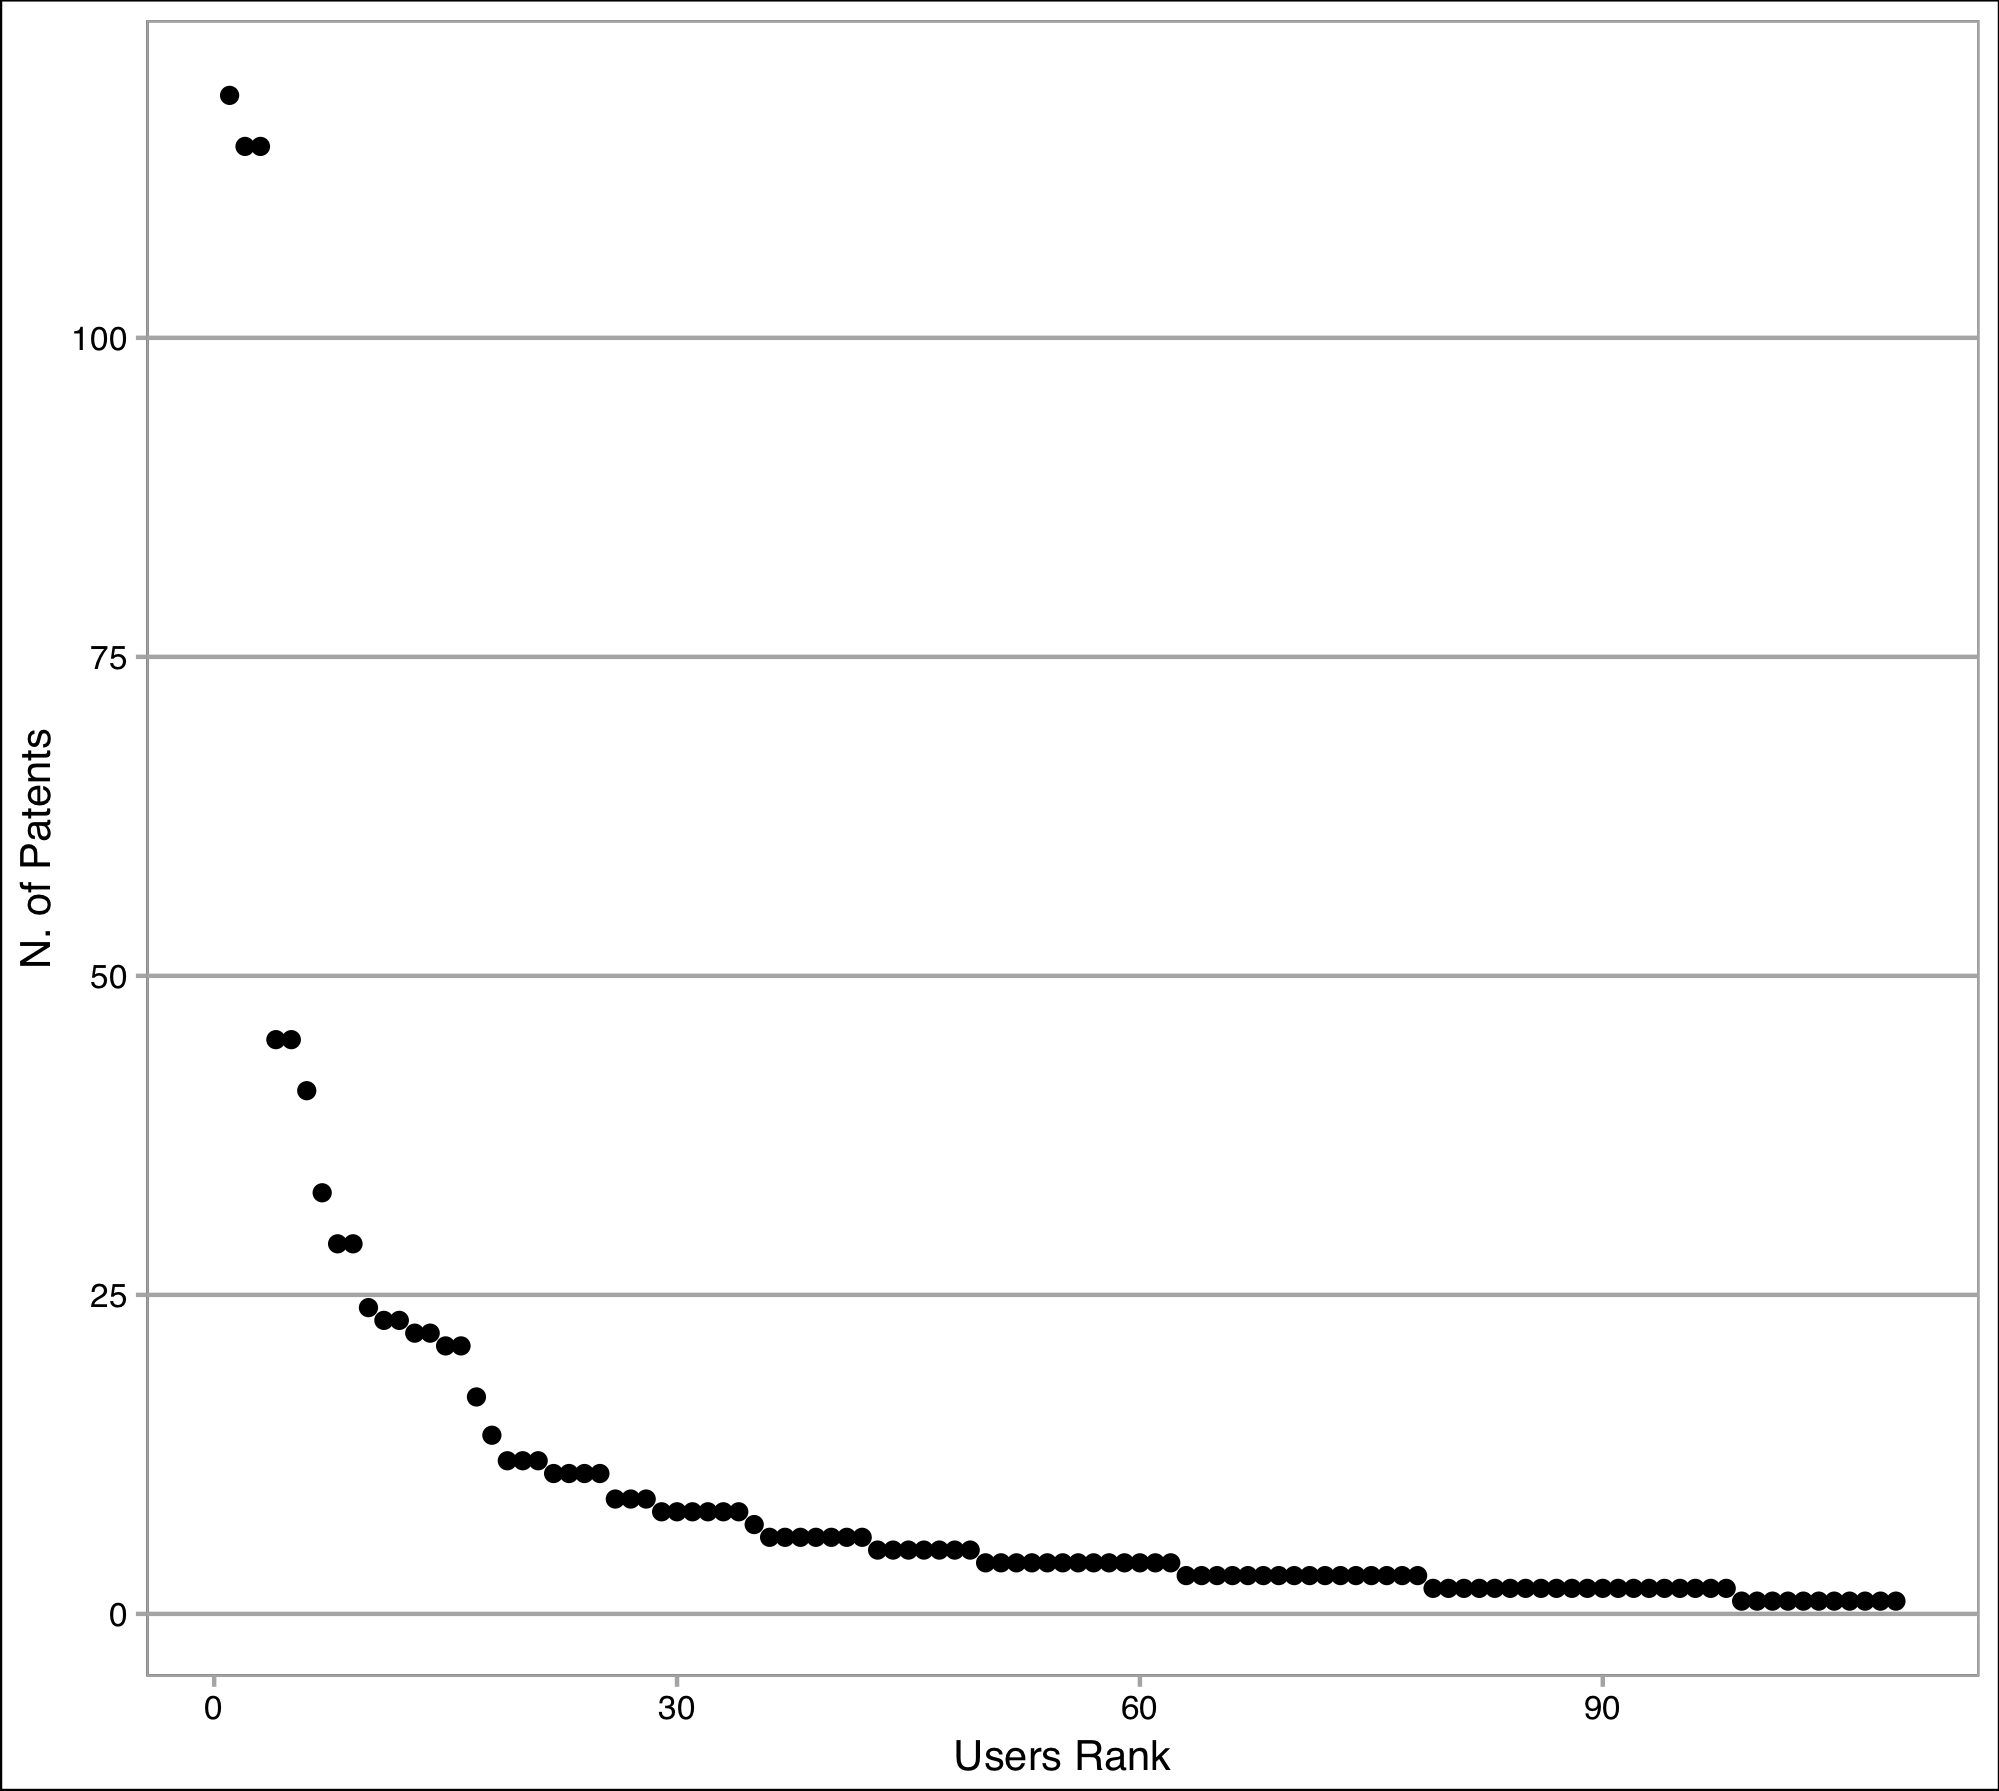
\includegraphics[width=0.6\linewidth]{_bookdown_files/figures/user_rank} 

}

\caption{Distribution of the number of patents per user.}\label{fig:patentsperuser}
\end{figure}

\section{Advantages and Drawbacks}\label{advdrwresults}

An effective development of new products or the redesign of an existing
one require the analysis of its positive and negative properties. Due to
that, advantages and drawbacks of products are extremely valuable
information for companies. Unfortunately, this information is not easy
to obtain and manage: a strong evidence of that is the effort in the
development of tools able to manage this information
\citep{pahl2013engineering, ulrich2003product}. Companies frequently
make use of Quality Functional Deployment (QFD) and requisites lists,
users' needs, users' requirements with the purpose of tracking
advantages \citep{carnevalli2008review}. On the other hand, companies
use Failure mode and effects analysis (FMEA) to gather and study
drawbacks, failure modes and their effects and causes
\citep{liu2013risk} However, product developers can acquire QFD and FMEA
data only from the users of the invention: this leads to the need of
expensive processes of customer's voice listening whose results are
often unclear. Moreover, this information is not disclosed to
researchers since this is part of the company know-how.

The description of the brought advantages and solved drawbacks are
critical requirements for the patentability of a product, as stated by
the politics and the guidelines given by World Intellectual Property
Organization (WIPO) on writing patents \citep{world2004wipo}. As stated
by WIPO, an invention is a \emph{solution} to a specific \emph{problem}
. The problem that an invention solves is a negative effect that
state-of-the-art technologies can not fully overcome; on the other side,
a solution is a way to solve this problem. A solution can lead to some
advantages with respect to the known art. Thus, starting from the
definition of invention, it is clear how it can be characterized by the
advantages that it brings and by the problems that it solves. Also, it
is reasonable to assume that having a clear picture of both advantages
and drawbacks of a technology is important for an effective design
process \footnote{The most precise couple of words is \textbf{advantage}
  and \textbf{disadvantage}, but the reading is facilitated by using two
  very different words, therefore we decided to adopt the couple
  \textbf{advantage} and \textbf{drawback}.}

\subsection{Methodology}\label{methodology}

In this section we show the approach used to extract the advantages and
the drawbacks of the invention described in a patent. More precisely,
the system identifies textual elements which represent the advantages or
the drawbacks described in a patent. Advantages and drawbacks
information can strongly advantage designers in the phase of new product
development or in the process of product improvement and marketers in
the phase of customer understanding and product placing. Furthermore a
patent based method has a strong advantage with respected to methods
that extracts information using other type of documents (e.g.~online
reviews of products \citep{monireh}): patents anticipate availability of
products on the market by a factor varying from 6 to 18 months
\citep{golzio2012}.

The proposed extraction process is shown in figure
\ref{fig:advdrwprocessgeneral} and its macro-phases are:

\begin{enumerate}
\def\labelenumi{\arabic{enumi}.}
\tightlist
\item
  \emph{Advantage and Drawback Clues Collection}: in this section we
  described the method to collect a reasonable number of generic
  advantage and drawback clues;
\item
  \emph{Domain Clues Extraction}: in this section is shown how the
  generic clues are used in exploiting machine learning algorithm to
  extract new domain specific advantages and drawback clues;
\item
  \emph{Domain Clues Validation} : since the new clues are automatically
  extracted, the output of the extraction phase surely contains a
  certain degree of noise. To clean this output a validation tool based
  on tweeter sentiment analysis is developed;
\item
  \emph{Advantages and Drawbacks Extraction}: here the extracted clues
  (generic and domain specific) are expanded according to specific
  regular expression pattern in order to obtain the advantages and the
  drawbacks of the analyzed patent set.
\end{enumerate}

\begin{figure}

{\centering 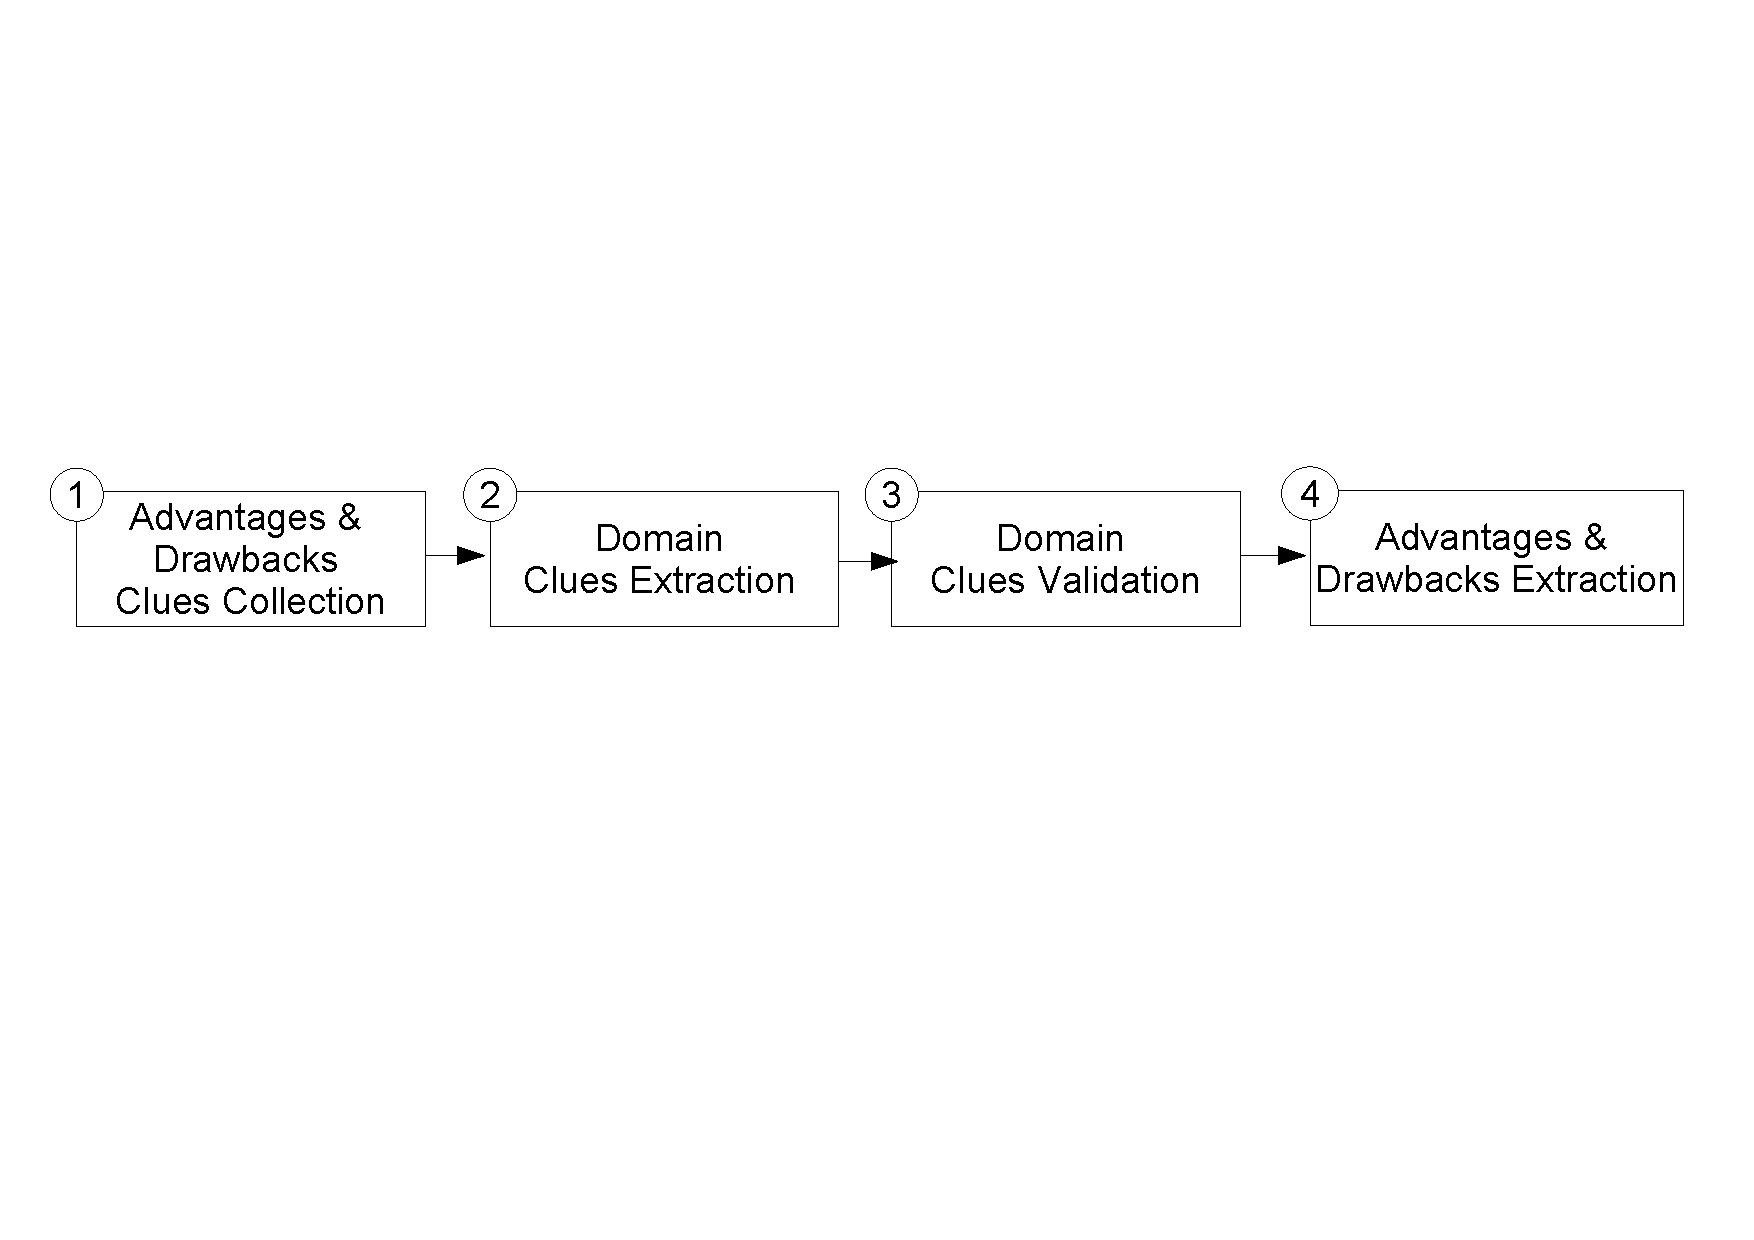
\includegraphics[width=0.8\linewidth]{_bookdown_files/figures/General} 

}

\caption{Main overview of the advantages and drawbacks extraction process from patents.}\label{fig:advdrwprocessgeneral}
\end{figure}

\subsubsection*{Clues of Advantages and drawbacks in
patents}\label{clues-of-advantages-and-drawbacks-in-patents}
\addcontentsline{toc}{subsubsection}{Clues of Advantages and drawbacks
in patents}

First of all we have to define the concept of clue to an advantage or a
drawback. To describe with a certain degree of precision an advantage or
a drawback, patent writers need to use sequences of words of a certain
length. Since NER systems do not perform well on long sequence of
tokens, we split the problem of extracting advantages and drawbacks in
two parts: first we extract entities that are clues in the sequence of
words that describes the advantage or the drawback; then we extract the
surrounding words to collect the whole sequence that describes the
advantage or the drawback.

To better understand these concepts some examples are:

\begin{itemize}
\item
   ease of access
\item
  cook food quickly and economically
\item
  benefits of keeping an outdoor cooker lid fixed
\end{itemize}

For the present work, we refer to advantages and drawbacks as a sequence
of words of minimal length that express the advantage or the drawback.
The three phrases of the example are three advantages. On the other hand
clues are words that are likely to be contained in advantages or
drawbacks phrases.

\subsubsection*{Advantages and Drawbacks Clue
Collection}\label{advantages-and-drawbacks-clue-collection}
\addcontentsline{toc}{subsubsection}{Advantages and Drawbacks Clue
Collection}

\begin{figure}

{\centering 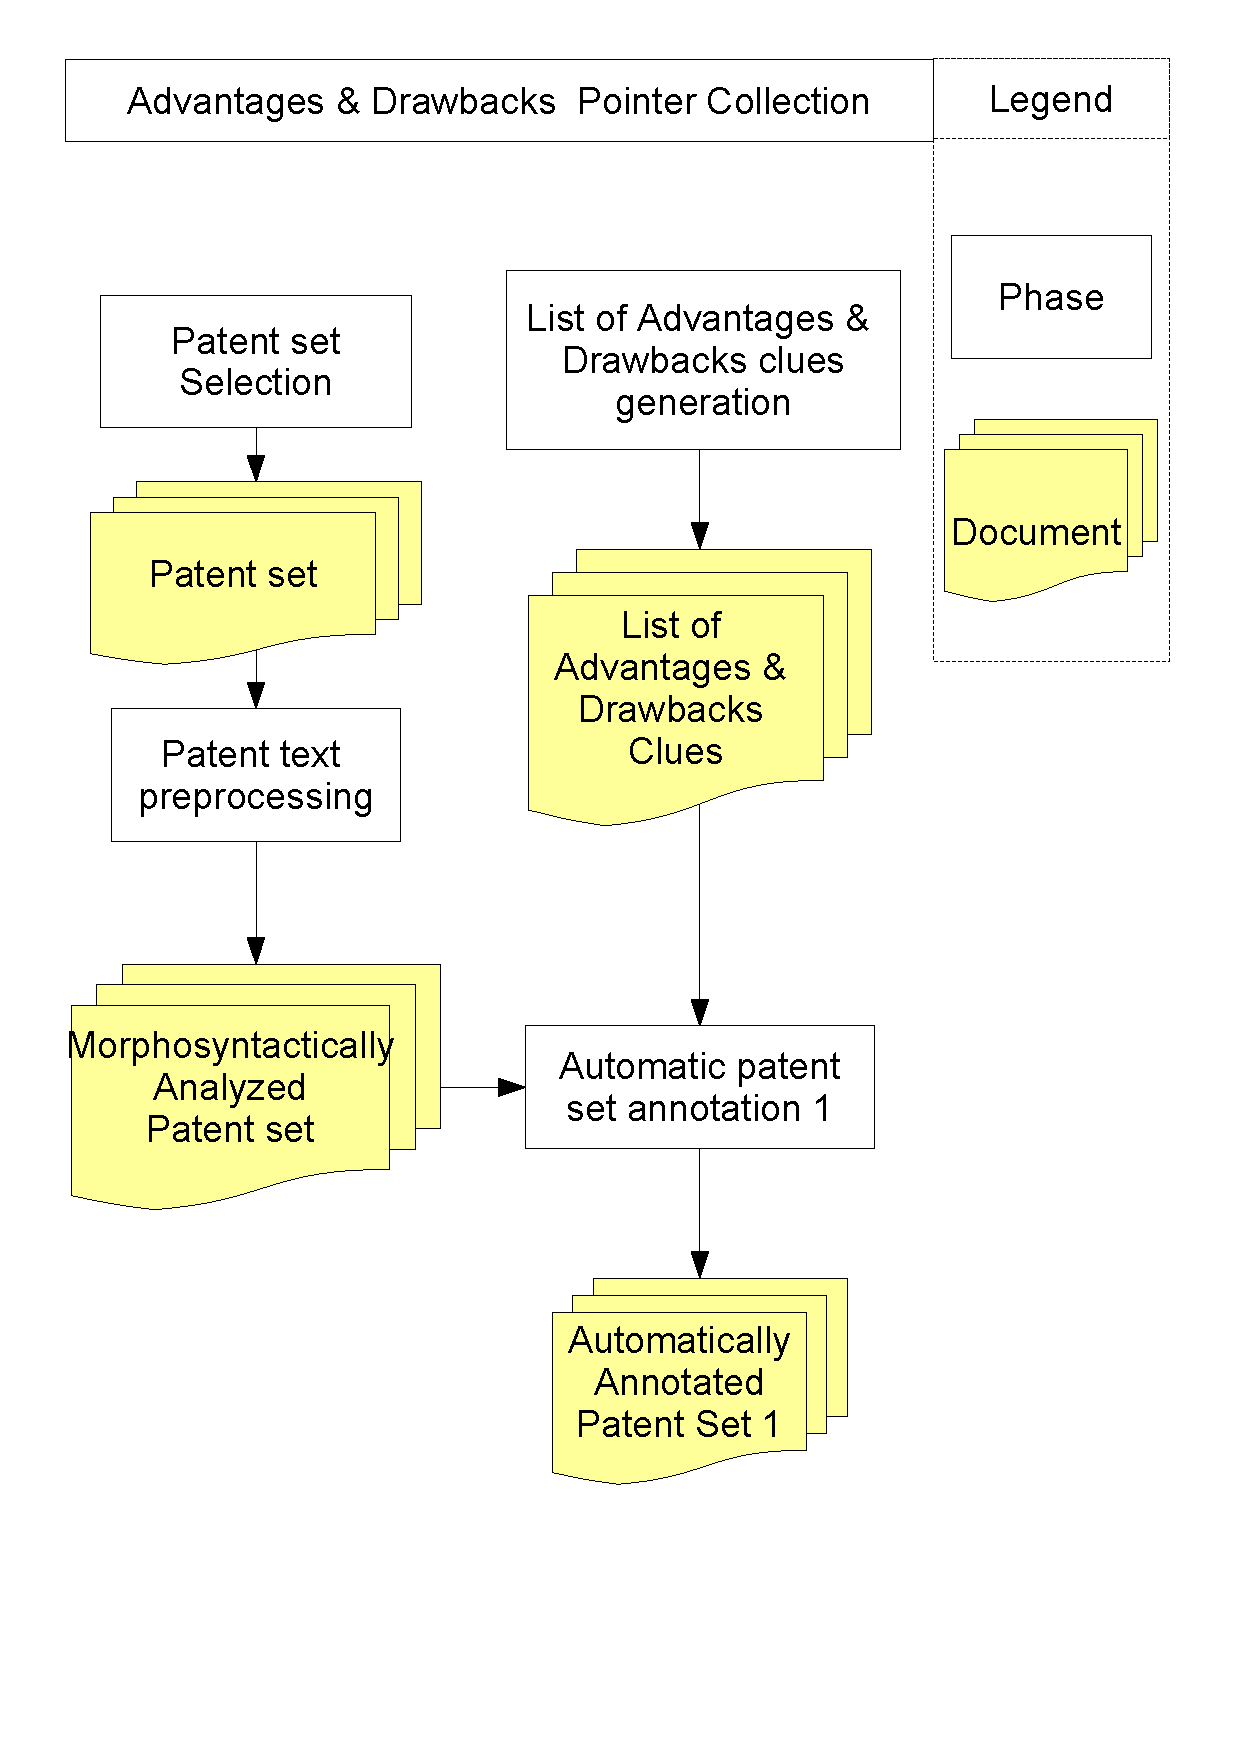
\includegraphics[width=0.8\linewidth]{_bookdown_files/figures/pointer-collection-phase} 

}

\caption{Main overview of the patent set annotation process.}\label{fig:advdrwarticlecluecollection}
\end{figure}

The approaches to generate a knowledge base of clues were two. The first
approach was based on a manual collection of clues of advantages and
drawbacks directly from patent texts. This process was performed on
2,000 patents, randomly chosen from the freepatent database \footnote{\url{http://www.freepatentsonline.com/}}.
With this approach we were able to collect 3,254 advantages and 5,142
drawback clues. Some examples of the extracted clues are shown in table
\ref{tab:advdrwarticleextdclue}.

\begin{longtable}[]{@{}cc@{}}
\caption{\label{tab:advdrwarticleextdclue} Examples of the clues collected
with the first approach.}\tabularnewline
\toprule
\emph{Advantages Clues} & \emph{Drawbacks Clues}\tabularnewline
\midrule
\endfirsthead
\toprule
\emph{Advantages Clues} & \emph{Drawbacks Clues}\tabularnewline
\midrule
\endhead
ability & aggravated\tabularnewline
efficacy & breakage\tabularnewline
ensure & damage\tabularnewline
healthy & defect\tabularnewline
innovative & error\tabularnewline
optimum & improper\tabularnewline
protect & leak\tabularnewline
quick-release & problem\tabularnewline
reinforce & unavailable\tabularnewline
securely & wrong\tabularnewline
\bottomrule
\end{longtable}

The second approach consisted in looking for alternative methods to
indicate advantages or drawbacks clues, looking defined word patterns.
The most relevant are the negations of advantages to obtain drawbacks,
and the negation of drawbacks to obtain advantages. Some examples of
such constructions are shown in table \ref{tab:advdrwarticleexbaclue}.

\begin{longtable}[]{@{}cc@{}}
\caption{\label{tab:advdrwarticleexbaclue} Examples of the clues collected
with the second approach.}\tabularnewline
\toprule
\emph{Advantages Clues} & \emph{Drawbacks Clues}\tabularnewline
\midrule
\endfirsthead
\toprule
\emph{Advantages Clues} & \emph{Drawbacks Clues}\tabularnewline
\midrule
\endhead
non damaged & out of\tabularnewline
anti-corrosion & in need of comfort\tabularnewline
loss reduction & non user-friendly\tabularnewline
prevent & diminish comfort\tabularnewline
defect free & issue with\tabularnewline
reduce waste & problem with\tabularnewline
reduction of & lacks of\tabularnewline
cost less & lacks with\tabularnewline
less severe & loss of\tabularnewline
avoid disease & unfacilitate\tabularnewline
\bottomrule
\end{longtable}

At the end of this process, a total of 6.568 advantages and the 14.809
drawbacks formed the knowledge base for the system, and gave us a
reasonable number of clues to be used in the next step of the process.

The first approach was restricted by the lists being extracted from a
random and limited sample of patents. On the other side, the rules used
in the second approach are non exhaustive, and this can create non-sense
clues, due to all of the possible combinations of words. Anyway, it is
reasonable to assume that a large set of non-domain dependent clues are
collected and will be used in the next steps of the process.

It is important to underline that the list of advantages and drawbacks
clues is designed to avoid linguistic ambiguities when projecting these
entities on the corpus. For example \emph{guide} has two different
meanings\footnote{www.dictionary.com} when used as a verb or as a noun:
as a verb it means \emph{``to assist something or someone to travel
through, or reach a destination in, an unfamiliar area, as by
accompanying or giving directions''}, so it could be the clue to an
advantage; at the same time as a noun it assumes the mean of \emph{``a
book, pamphlet, etc., giving information, instructions, or advice;
handbook''} thus indicating a product and not an advantage. Avoiding
such ambiguities is a crucial aspect to produce an informative training
set, so ambiguous words were avoided to be projected on patents.

\subsubsection*{Domain Clues Extraction}\label{domain-clues-extraction}
\addcontentsline{toc}{subsubsection}{Domain Clues Extraction}

The domain-specific clues collection process takes in input the
automatically annotated patent set 1. The analyzed patent set is
automatically annotated using the domain-independent clues, and is used
to extract new domain-specific clues. We decided for the present methods
to analyze the whole text of the patents and not to focus only on a
specific section.

\begin{figure}

{\centering 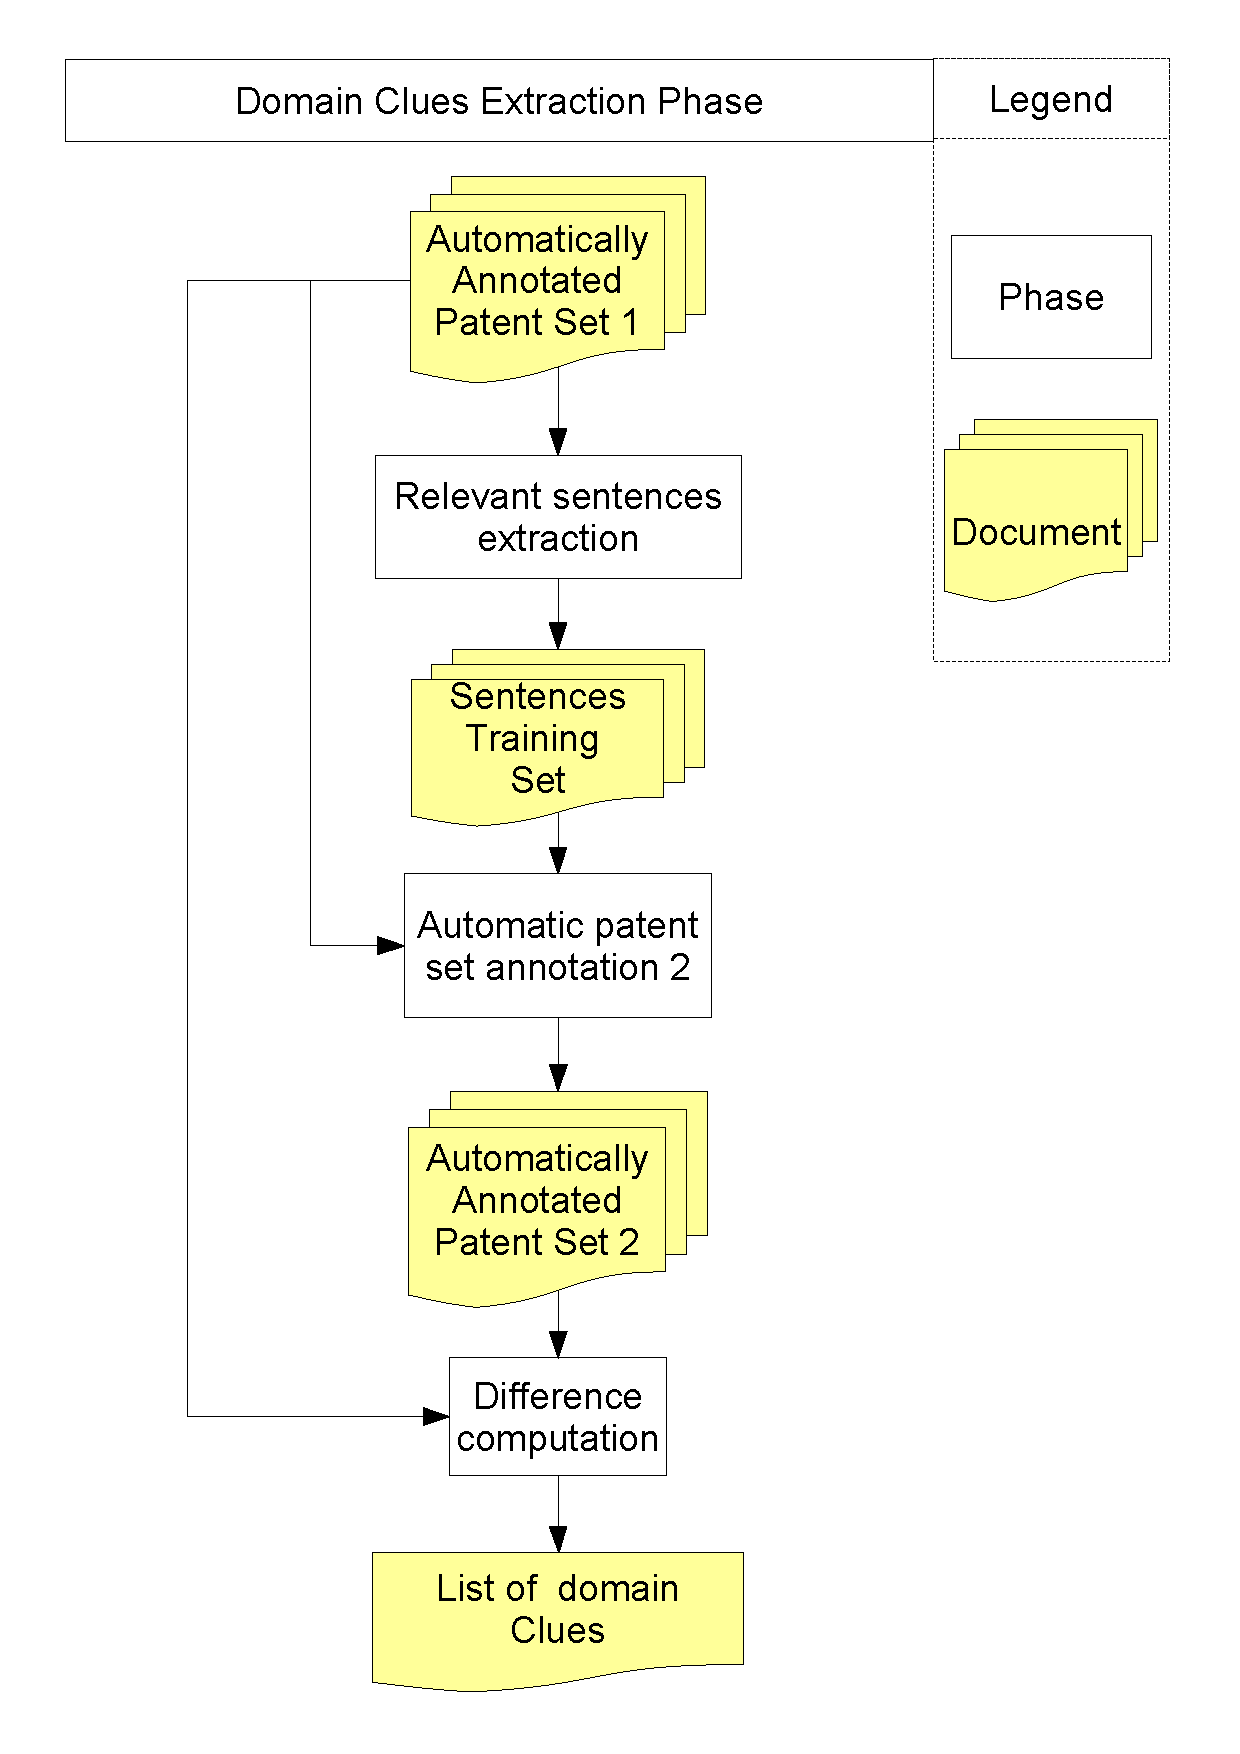
\includegraphics[width=0.8\linewidth]{_bookdown_files/figures/pointer-expansion-phase} 

}

\caption{Overview of the domain specific advantages and failures clues extraction process.}\label{fig:advdrwarticleprocessfigclueexpansionphase}
\end{figure}

Our system resorts to state-of-the-art NLP tools which are part of the
linguistic analysis pipeline shown in figure
\ref{fig:advdrwarticleprocessfigclueexpansionphase}. In addition we
developed a specific advantages and drawbacks clues extraction tool,
still based on Natural Language Processing techniques.

The automatic patent set annotation 2 process, as shown in figure
\ref{fig:advdrwarticleprocessfigclueexpansionphase}, is composed by a
set of sequential steps. The first three steps are related to the
linguistic annotation: sentence splitting and tokenization, part of
speech tagging and lemmatization. Once these three steps are completed
the entity extractor collects the advantages and drawbacks clues from
the analyzed patents.

\emph{Sentence splitting and Tokenization} steps split the text into
sentences and then segment each sentence in orthographic units called
tokens.

The \emph{Part-Of-Speech tagging} (or POS tagging) step assigns
unambiguous grammatical categories to the tokens. For the present
application we use the most recent version of the Felice-POS-tagger
described in \citep{dell2009ensemble}. Once the computation of the
POS-tagged text is completed, the text is automatically
\emph{lemmatized} in order to group inflected forms of a word in a
single item. Some of the following steps of the entire extraction
process exploit the lemmatized texts in order to achieve better
extraction results.

Successively the \emph{semi-automatic annotation of advantages and
drawbacks clues} is performed. The advantages and drawbacks clues
extraction tool is the key ingredient of the present thesis, and it is
based on supervised methods. Such methods require an entity annotated
corpus in order to extract new entities from unseen documents. Since the
manual annotation of a patent set is too expensive both in terms of time
and manual effort, we apply a semi-automatic method to generate an
advantage and drawback annotated corpus.

The entity annotation schema for a single token is defined using a
widely accepted BIO annotation scheme \citep{ramshaw}:

\begin{itemize}
\tightlist
\item
  \textbf{B-ADV}: the token is the start of an entity representing an
  advantage clue;
\item
  \textbf{I-ADV}: the token is the continuation of a sequence of tokens
  representing an advantage clue;
\item
  \textbf{B-DRW}: the token is the start of an entity representing a
  drawback clue;
\item
  \textbf{I-DRW}: the token is the continuation of a sequence of tokens
  representing a drawback clue;
\item
  \textbf{O}: for the remaining case.
\end{itemize}

The \emph{Advantages and Drawbacks Clues Extractor} is a supervised
classifier that, given an annotated patent set, is trained on these
examples. The patent set is: (a) linguistically-annotated, using the
steps described above; (b) entity-annotated, exploiting the
semiautomatic annotation process executed in the previous steps. Given a
set of features the classifier trains a statistical model using the
feature statistics extracted from the corpus. This trained model is then
employed in the classification of unseen patents: it extracts new domain
specific clues from patents and assigns them a probability score whether
they are an advantage or a drawback. In our experiments the classifier
has been trained using the Support Vector Machines (SVM) learning
algorithm using the LIBSVM \citep{svm} library configured to use a
linear kernel. The classifier uses two different kinds of features that
are extracted from the text:

\begin{itemize}
\item
  \textbf{raw features}: prefix and suffix of the analyzed token; it
  works particularly well with advantages ending with -full -ious and
  with drawbacks starting with un- dis- etc..
\item
  \textbf{word2vec features}: vector representations of words computed
  by the \emph{word2vec} \citep{word2vec1} tool.
\end{itemize}

Table \ref{tab:featconfsadvdis} reports the detailed features chosen for
the proposed advantage and drawbacks clues extractor.

\begin{longtable}[]{@{}cc@{}}
\caption{\label{tab:featconfsadvdis} Context windows of the extracted
features considering 0 as the current analyzed token.}\tabularnewline
\toprule
\emph{Feature group} & \emph{Context Window}\tabularnewline
\midrule
\endfirsthead
\toprule
\emph{Feature group} & \emph{Context Window}\tabularnewline
\midrule
\endhead
Prefixes up to 4 & \(0\)\tabularnewline
Suffixes up to 4 & \(0\)\tabularnewline
Word2vec & \(-2, -1, 0, 1, 2\)\tabularnewline
TAG & \(-1\)\tabularnewline
\bottomrule
\end{longtable}

By introducing prefixes and suffixes of the analyzed token, the
classifier is able to identify frequent orthographic patterns which
allow to maximize the precision in classification phase. On the other
hand, the \emph{word2vec} features are introduced in order to maximize
the recall, since semantically similar clues should have similar
\emph{word2vec} vectors. Finally, the tag of the previous token is added
to the final feature vector in order to improve the accuracy
classification of multi-word clues.

\subsubsection*{Word2vec feature
computation}\label{word2vec-feature-computation}
\addcontentsline{toc}{subsubsection}{Word2vec feature computation}

While contextual, linguistic and compositional features are commonly
used for entity extraction task in patents, from a computational
linguistic point of view the presented system introduces the novelty of
using \emph{word2vec} features for entity extraction in patents.

\emph{Word2vec} is a NLP tool able to produce word representations
exploiting big corpora. The main property of the vectors produced by
\emph{word2vec} is that words that share similar contexts have similar
vector representations. By using word vectors instead of the
corresponding words we were able to overcome the problem of the limited
lexical knowledge in the training phase.

To build our \emph{word2vec} vectors we used the Skipgram model with a
context window of 5 tokens. As reported in table
\ref{tab:word2vecpatents}, we used a corpus consisting of 48,194
different patents, containing more than 400,000,000 tokens.

The corpus was designed to contain patents belonging to different
classes (12 in total) in order to acquire an extended knowledge of the
contexts in which the words in general are surrounded. In addition,
patents belonging to two of these classes are analyzed and, in the same
section, detailed configurations of the entity extractor has been
provided.

\begin{longtable}[]{@{}ccc@{}}
\caption{\label{tab:word2vecpatents} Statistics of the documents on which
the word2vec vectors have been learned. The patent sets of the analyzed
case study are reported in bold.}\tabularnewline
\toprule
Patent class & \# Patents & \# Tokens\tabularnewline
\midrule
\endfirsthead
\toprule
Patent class & \# Patents & \# Tokens\tabularnewline
\midrule
\endhead
\textbf{A47G33} & \textbf{2423} & \textbf{5.225.000}\tabularnewline
\textbf{A61G13} & \textbf{2991} & \textbf{15.937.000}\tabularnewline
\textbf{A61G1} & \textbf{5040} & \textbf{36.348.000}\tabularnewline
\textbf{A61H} & \textbf{5199} & \textbf{41.831.000}\tabularnewline
A61P25/24 & 5297 & 103.098.000\tabularnewline
A63F1 & 5461 & 75.900.000\tabularnewline
A63F3 & 4923 & 40.909.000\tabularnewline
A63F7 & 4747 & 13.807.000\tabularnewline
E02B3 & 3796 & 14.434.000\tabularnewline
E04H9 & 2221 & 12.500.000\tabularnewline
G01V11 & 1345 & 11.166.000\tabularnewline
G08B13 & 4831 & 40.904.000\tabularnewline
\emph{Total} & 48194 & 412.065.000\tabularnewline
\bottomrule
\end{longtable}

\subsubsection*{Clue validation using tweets sentiment
analysis}\label{clue-validation-using-tweets-sentiment-analysis}
\addcontentsline{toc}{subsubsection}{Clue validation using tweets
sentiment analysis}

\begin{figure}

{\centering 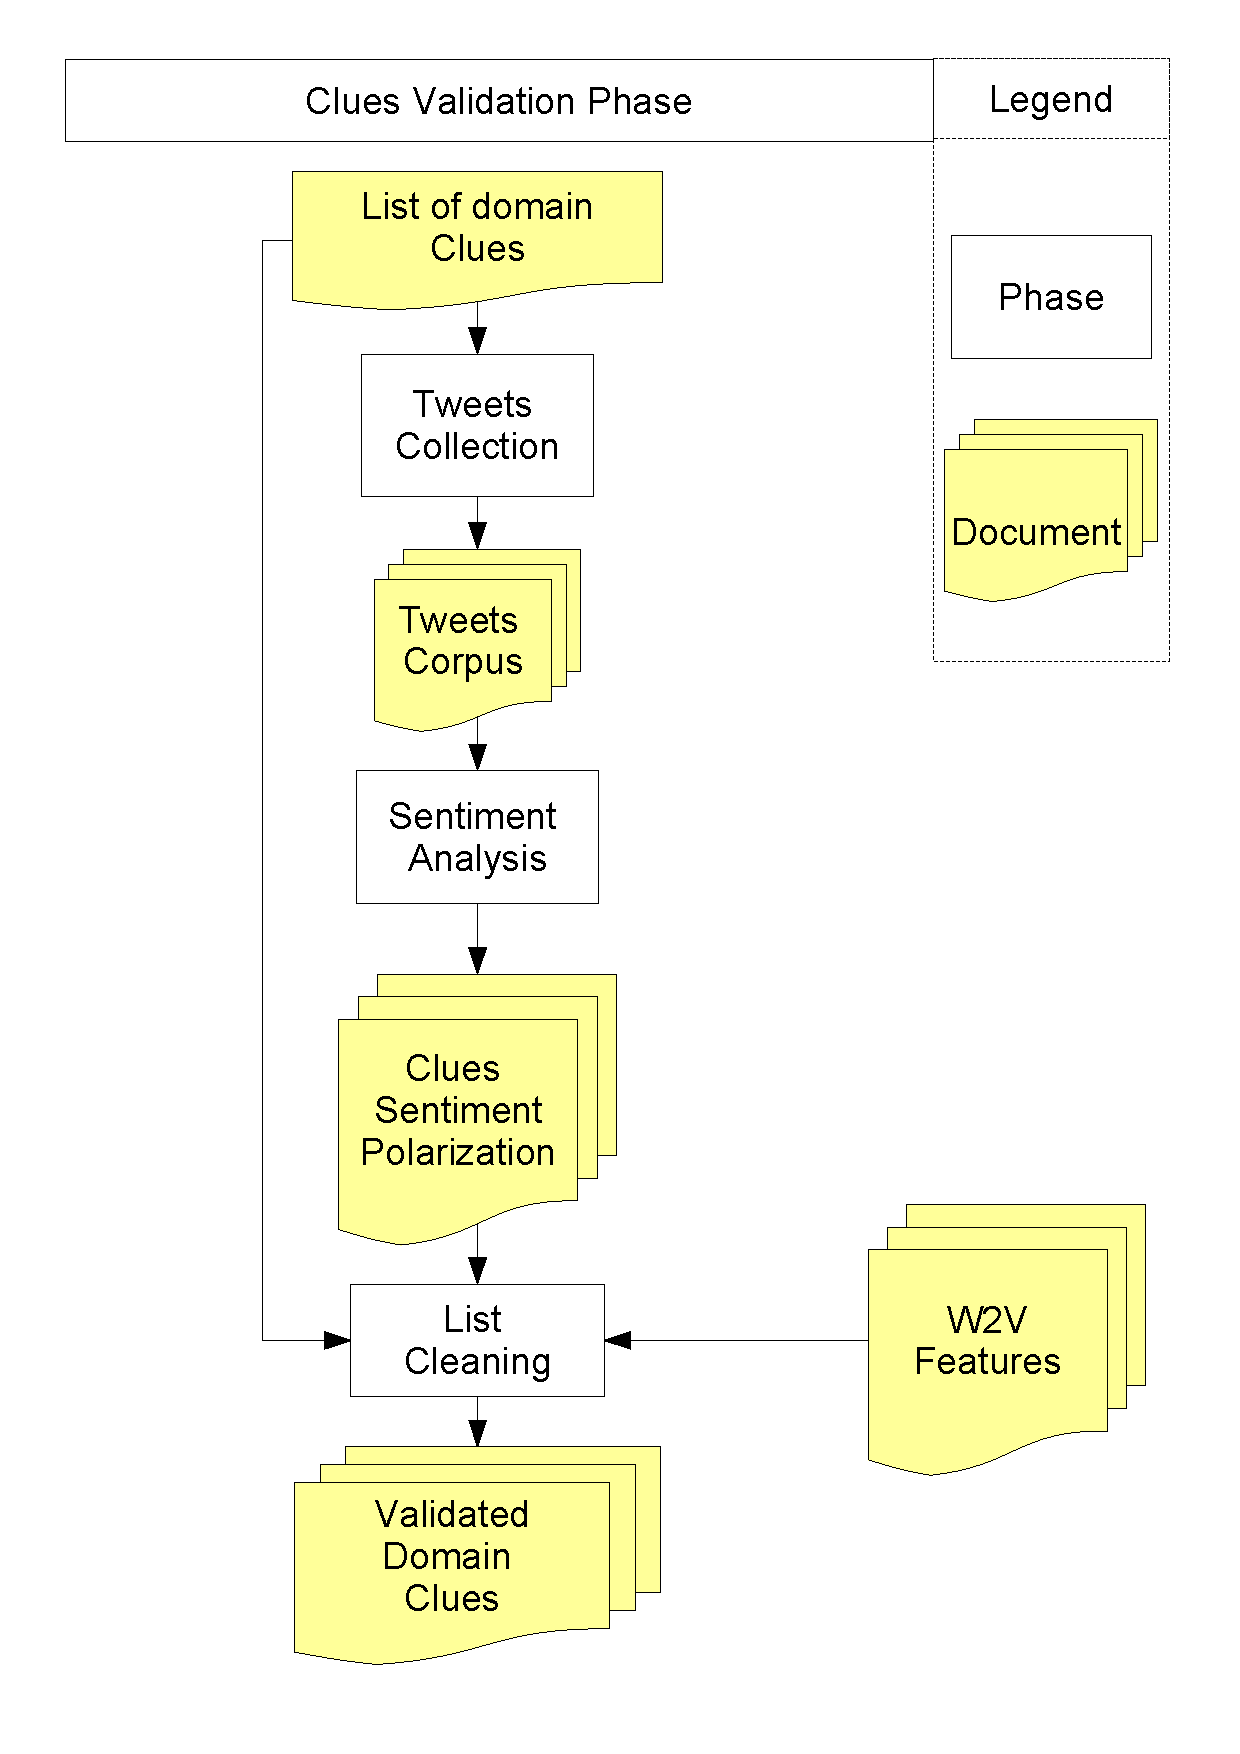
\includegraphics[width=0.8\linewidth]{_bookdown_files/figures/pointer-validation-phase} 

}

\caption{Overview of the domain specific advantages and failures clue validation process.}\label{fig:advdrwarticleprocessfigcluevalidationphase}
\end{figure}

Figure \ref{fig:advdrwarticleprocessfigcluevalidationphase} gives an
overview of the activities performed to validate the collected clues
using twtitter. Since the manual review of the new domain specific clues
can be very time consuming, an innovative approach to automatic
validation of these entities is proposed. The approach is based on the
assumption that advantages of technological innovations can be
considered positive factors by the users. Conversely, the drawbacks of
the artifacts are considered negative factors impacting on the
satisfaction of the users. Both advantages and drawbacks are common
terms or chunks of terms commonly used in other contexts, too.
Therefore, if we can identify a wide source of sentences tagged with a
polarity score and containing advantages or drawbacks, the probability
of assigning the proper polarity to advantages and drawbacks increases.
Of course this method has a treat: some technical words can be used
rarely in a non-technical context. For this reason we will rely on a big
number of tweets in order to augment the probability of finding all the
clues we want to measure.

Social media platforms provide powerful venues for consumers to interact
not only with brands but also with other consumers as they engage in the
processes of curation, creation, and collaboration
\citep{evans2010social}. Such virtual platforms are places where users
discuss about products, about their features but also about problems and
failures they experienced during the daily use. The way they discuss or
describe products or services is often unambiguous and highly polarized.

Our approach to the automatic validation of advantages and drawbacks
exploits the information contained in the Twitter platform \footnote{\url{https://twitter.com}}.
More precisely, for each extracted advantage or drawback clue we collect
a set of tweets in which the clue is mentioned. Once a significant
number of tweets is collected (in our case 3,073,959 - around 2,738 per
entity in average), they are analyzed by a sentiment classifier. The
main idea behind this process is to assign to each clue a sentiment
polarity score which should express the feeling of the user with respect
to the considered clue on the social media.

The tweet collection can be easily performed by using the Twitter
streaming API \footnote{\url{https://dev.twitter.com/streaming/public}},
which is freely available. By assigning a polarity score to each clue,
we expect to detect tagging anomalies: entities tagged as advantages by
the classifier are expected to have a positive polarity in the extracted
tweets. Vice versa, entities tagged as drawbacks by the classifier are
expected to have a negative polarity in the extracted tweets.

\subsubsection*{Sentiment Classifier: features, classification model and
performance
evaluation}\label{sentiment-classifier-features-classification-model-and-performance-evaluation}
\addcontentsline{toc}{subsubsection}{Sentiment Classifier: features,
classification model and performance evaluation}

In our sentiment classifier we focused on a wide set of features ranging
across different levels of linguistic description. The whole set of
features we started with is described below, organized into four main
categories:

\begin{itemize}
\tightlist
\item
  raw and lexical text features
\item
  morpho-syntactic features
\item
  syntactic features
\item
  lexicon features.
\end{itemize}

This proposed four-fold partition closely follows the different levels
of linguistic analysis which is automatically carried out on the text
being evaluated, (i.e.~tokenization, lemmatization, morpho-syntactic
tagging and dependency parsing) and the use of external lexical
resources.

Raw and lexical text features are extracted considering the text
available in the tweet. For this work we considered a number of tokens,
character n-grams, word n-grams, lemma n-grams, char repetition
sequences, mentions number, hashtags number and punctuation.

Morpho-syntactic and Syntactic Features consider the part of speech tags
and the syntactic analysis of the text. Our sentiment analyzer extracts
Part-Of-Speech n-grams (coarse and fine), coarse grained Part-Of-Speech
distribution and syntactic dependency types n-grams.

To extract features based on lexicons we exploited three freely
available resources. The Bing Liu Lexicon \citep{hu2004mining}, which
includes approximately 6,000 English words, the Multi--Perspective
Question Answering Subjectivity Lexicon \citep{wilson2005recognizing},
which consists of approximately 8,200 English words and the SentiWordNet
3.0 Lexicon \citep{baccianella2010sentiwordnet} which consists of more
than 117,000 words. For each word in these lexicons the associated
polarity is provided. In addition, we manually developed a lexicon of
positive and negative emoticons, which usually is a strong indicator of
tweets polarity. By exploiting the described resources, the following
features were extracted: positive/negative emoticon distribution,
sentiment polarity n-grams, sentiment polarity modifiers, the
distribution of sentiment polarity, the most frequent sentiment polarity
and changes of polarity in tweet sections. A more detailed description
of these features is provided in {[}\citet{cimino2014linguistically}.

In order to assign a sentiment polarity score to each tweet, we employed
an adapted version of the ItaliaNLP Sentiment Polarity Classifier for
the English language \citep{cimino2014linguistically}. This classifier
operates on morpho-syntactically tagged and dependency parsed texts and
assigns to each document a score expressing its probability of belonging
to a given polarity class. The highest score represents the most
probable class. Given a set of features and a training corpus, the
classifier creates a statistical model using the feature statistics
extracted from the training corpus. This model is used in the
classification of unseen documents. The set of features and the machine
learning algorithm can be parametrized through a configuration file. For
this work, we used a tandem Long Short Term Memory Recurrent Neural
Network (LSTM) - Support Vector Machines (SVM) architecture.

\subsubsection*{Filterting and validation of the extracted
clues}\label{filterting-and-validation-of-the-extracted-clues}
\addcontentsline{toc}{subsubsection}{Filterting and validation of the
extracted clues}

The sentiment classifier is employed to validate the advantage and
drawback clues which were previously extracted from patents by the clue
extractor. In order to do so, we exploited the output of the tweet
classifier on the tweets we previously downloaded. Each tweet, as said
before, contains one or more clues to be validated. The sentiment
classifier assigns the likeliness to each tweet to positive, neutral or
negative. Consequently by analyzing all the tweets we previously
downloaded, we obtained for each clue the distribution of positive,
neutral and negative tweets.

Then to make a decision regarding each clue we used another SVM based
classifier. This classifier is trained on a gold set of advantages and
drawbacks clues: we manually labeled 344 words as advantages and 193
words as drawbacks, obtaining the gold set. The features used by this
classifier are a number of positive, neutral and negative tweets
extracted in which the entities are mentioned and the \emph{word2vec}
vector representing the considered entity.

The classification results of the proposed approach over a 5-fold cross
validation using the SVM-W2V are:

\begin{itemize}
\tightlist
\item
  Global accuracy: 87.71
\item
  ADV Precision: 89.89
\item
  ADV Recall: 91.29
\item
  DRW Precision: 83.35
\item
  DRW Recall: 80.66
\end{itemize}

The obtained results show that the proposed entity validation method is
suitable for the automatic advantages/drawbacks clues validation
process.

\subsubsection*{Advantages and Drawbacks sentences
extraction}\label{advantages-and-drawbacks-sentences-extraction}
\addcontentsline{toc}{subsubsection}{Advantages and Drawbacks sentences
extraction}

\begin{figure}

{\centering 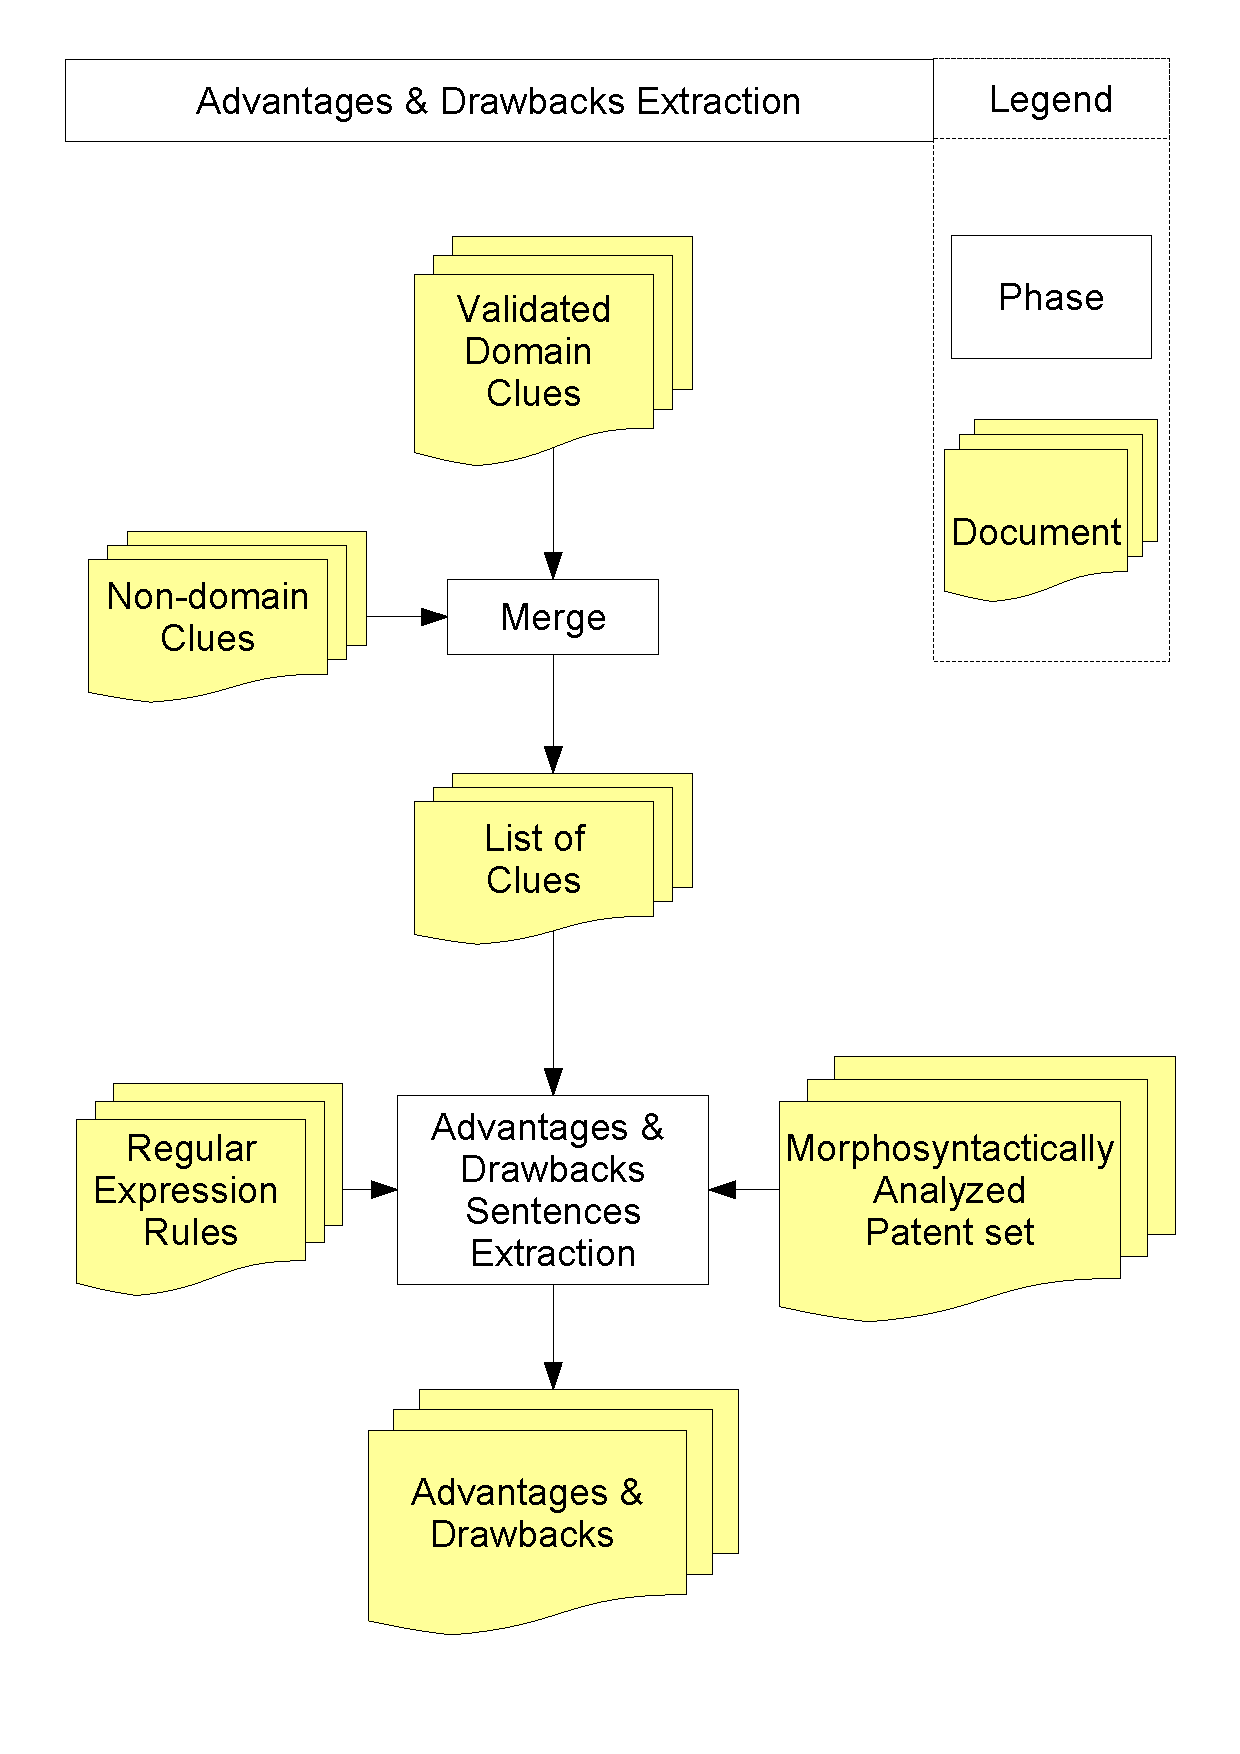
\includegraphics[width=0.8\linewidth]{_bookdown_files/figures/relevant-sentences-extraction} 

}

\caption{Overview of the advantages and failures extraction process.}\label{fig:advantagedrawbacksextraction}
\end{figure}

The advantages and drawbacks extraction process is shown in figure
\ref{fig:advantagedrawbacksextraction}. Once all the domain specific
advantages and drawbacks clues are extracted, these are merged with the
ones belonging to the original knowledge base, obtaining a final list
which will be processed by the advantages and drawbacks sentences
extractor. The advantages and drawbacks sentences extractor exploits
predefined linguistic and clues filters which operate on the automatic
pos--tagged patents. Specifically, for each advantage and drawback term
identified in patents, we used a pos--clue-pattern constraining the
start-token and the rest of the token pos. Since we were interested in
phrases containing words belonging to specific morphological categories,
we identified sequences of allowed pos--clue-pattern in order to cover
most of the English morphosyntactic multi--words structures, using the
following pattern:

(ADVClue\textbar{} DISClue)+Noun.*Noun.*Noun.

The pattern is applied to the previously lemmatized text in order to
have less sparse and more informative extractions.

This choice was made because the pattern:

\begin{enumerate}
\def\labelenumi{\arabic{enumi}.}
\tightlist
\item
  expresses an advantage or a drawback exhaustively;
\item
  increases the precision and the recall of the final output list of
  advantages and drawbacks;
\item
  allows to build a three-level named based tree over the final output
  list.
\end{enumerate}

In particular, the tree is built by grouping terms which share at the
first level the same clue, at the second level the same noun and at the
third level the same noun. This grouping procedure allows to easily
represent the final output list in a tree structure which can be easily
navigated by the end user of the system.

\subsection{Results}\label{results-1}

In this section we describe the experimental use of the proposed process
by applying it on four different patent sets.

To test the proposed methodology, we chose 4 patent sets composed of a
sample of 3,000 patents each. The patent sets belong to 4 different IPC
patent classes. The chosen classes and the definitions given by WIPO are
reported in table \ref{tab:advdrwarticleexampleipcclasses}.

\begin{longtable}[]{@{}cc@{}}
\caption{\label{tab:advdrwarticleexampleipcclasses} The patent IPC classes
from which samples of 3,000 patents were chosen for the experimental
analysis.}\tabularnewline
\toprule
\emph{IPC name} & \emph{Definition}\tabularnewline
\midrule
\endfirsthead
\toprule
\emph{IPC name} & \emph{Definition}\tabularnewline
\midrule
\endhead
A61G13 & Operating tables and auxiliary appliances
therefor\tabularnewline
A61H & Physical therapy apparatus\tabularnewline
A61C15 & Devices for cleaning between the teeth\tabularnewline
A47J37 & Baking; Roasting; Grilling; Frying\tabularnewline
\bottomrule
\end{longtable}

Our choice of patent sets aimed at challenging our system to find new
domain specific advantages and drawback clues in different domains.
Furthermore, we only selected patent sets from the IPC class A, which is
based on human necessities, to maximize the probability of finding
advantages and drawbacks that impacts on the users and not only on other
products/components.

Once the advantages and drawbacks are extracted, a manual review process
was performed on the output of the system to compute the number of true
positive clues. In this way we were able to compute the precision of the
process for both the advantages and the drawbacks. The output of the
clue extraction validated by the clue validator is analyzed in table
\ref{tab:advdrwarticlecluemeas}.

The table shows that the number of the extracted true positive advantage
clues is higher than the number of the extracted true positive drawback
clues. On the other side, the automatic evaluation process has a lower
performance on advantage clues in terms of precision.

A first hypotheses to explain these results is that our knowledge base
contained more drawback clues than advantage clues. Another possible
reason could be that the applicant is minded to describe the invention
highlighting the positive effects of the invention.

\begin{longtable}[]{@{}ccc@{}}
\caption{\label{tab:advdrwarticlecluemeas} Number of clues filtered with the
clue validator and number of true positive clues.}\tabularnewline
\toprule
& \# \emph{Advantage clues} & \# \emph{Drawbacks clues}\tabularnewline
\midrule
\endfirsthead
\toprule
& \# \emph{Advantage clues} & \# \emph{Drawbacks clues}\tabularnewline
\midrule
\endhead
\emph{Tot extracted clues} & 3607 & 1244\tabularnewline
\emph{Automatically Validated clues} & 1976 & 576\tabularnewline
\emph{True Positive} & 984 & 448\tabularnewline
\emph{Precision} & 49.8\% & 77.8\%\tabularnewline
\bottomrule
\end{longtable}

In order to assess the performance of the overall process, another
important measure is the amount of new information that is obtained,
which we call \emph{information gain}. As shown in table
\ref{tab:infogain1}, the percentage of new discovered clues decreases
with the number of starting clues. Obviously, the more patent sets are
analyzed, the less new generic and domain specific clues are extracted.
The percentage of information gain (represented as delta in the table),
stabilizes at a 5\% value in the advantage clues case, and 1\% in the
drawback clues case. This trend could be an evidence that the clue
extraction process has a natural saturation level.

\begin{longtable}[]{@{}ccccc@{}}
\caption{\label{tab:infogain1} Information gained by applying the extraction
process on different patent sets. Each row reports the percentage of
information gained by incrementally adding the extracted entities to the
knowledge base and the overall number of entities belonging to the
extended knowledge base.}\tabularnewline
\toprule
\emph{Patent set} & ∆ Adv. & \# Adv. & ∆ Draw. & \# Draw.\tabularnewline
\midrule
\endfirsthead
\toprule
\emph{Patent set} & ∆ Adv. & \# Adv. & ∆ Draw. & \# Draw.\tabularnewline
\midrule
\endhead
Knowledge Base & N/A & 6,568 & N/A & 14,809\tabularnewline
A47J33 & +23\% & 8,133 & +3\% & 15,332\tabularnewline
A61C15 & +12\% & 9,178 & +2\% & 15,644\tabularnewline
A61G13 & +5\% & 9,653 & +1\% & 15,849\tabularnewline
A61H & +5\% & 10,175 & +1\% & 16,053\tabularnewline
\bottomrule
\end{longtable}

Tables \ref{tab:advantageclueextracted} and
\ref{tab:drawbacksclueextracted} show the frequencies of a randomly
chosen set of the new extracted advantages and drawbacks domain specific
clues for each of the four analyzed patent sets. The results show that
the domain specific clues clearly characterize the different technical
areas of the patent sets. It is thus interesting to notice how valuable
information is contained in the context specific clues them self.
Further research can decide to stop here the process, without extracting
the whole sentence.

\begin{longtable}[]{@{}cccc@{}}
\caption{\label{tab:advantageclueextracted} Extracted domain specific
advantages clues with the measures of occurrences for each patent
set.}\tabularnewline
\toprule
\begin{minipage}[t]{0.16\columnwidth}\centering\strut
A47J37 (Baking)\strut
\end{minipage} & \begin{minipage}[t]{0.24\columnwidth}\centering\strut
A61H (Therapy apparatus)\strut
\end{minipage} & \begin{minipage}[t]{0.23\columnwidth}\centering\strut
A61C15 (Teeth cleaning)\strut
\end{minipage} & \begin{minipage}[t]{0.25\columnwidth}\centering\strut
A61G13 (Operating tables)\strut
\end{minipage}\tabularnewline
\begin{minipage}[t]{0.16\columnwidth}\centering\strut
transport 295\strut
\end{minipage} & \begin{minipage}[t]{0.24\columnwidth}\centering\strut
regenerative 144\strut
\end{minipage} & \begin{minipage}[t]{0.23\columnwidth}\centering\strut
elasticity 495\strut
\end{minipage} & \begin{minipage}[t]{0.25\columnwidth}\centering\strut
rigidity 784\strut
\end{minipage}\tabularnewline
\begin{minipage}[t]{0.16\columnwidth}\centering\strut
integrity 246\strut
\end{minipage} & \begin{minipage}[t]{0.24\columnwidth}\centering\strut
waterproof 101\strut
\end{minipage} & \begin{minipage}[t]{0.23\columnwidth}\centering\strut
rigidity 461\strut
\end{minipage} & \begin{minipage}[t]{0.25\columnwidth}\centering\strut
ventilation 177\strut
\end{minipage}\tabularnewline
\begin{minipage}[t]{0.16\columnwidth}\centering\strut
rigidity 233\strut
\end{minipage} & \begin{minipage}[t]{0.24\columnwidth}\centering\strut
hygienic 85\strut
\end{minipage} & \begin{minipage}[t]{0.23\columnwidth}\centering\strut
disinfection 247\strut
\end{minipage} & \begin{minipage}[t]{0.25\columnwidth}\centering\strut
hygiene 135\strut
\end{minipage}\tabularnewline
\begin{minipage}[t]{0.16\columnwidth}\centering\strut
insure 180\strut
\end{minipage} & \begin{minipage}[t]{0.24\columnwidth}\centering\strut
ergonomically 77\strut
\end{minipage} & \begin{minipage}[t]{0.23\columnwidth}\centering\strut
precision 199\strut
\end{minipage} & \begin{minipage}[t]{0.25\columnwidth}\centering\strut
versatility 121\strut
\end{minipage}\tabularnewline
\begin{minipage}[t]{0.16\columnwidth}\centering\strut
adjusting 164\strut
\end{minipage} & \begin{minipage}[t]{0.24\columnwidth}\centering\strut
disinfection 48\strut
\end{minipage} & \begin{minipage}[t]{0.23\columnwidth}\centering\strut
ergonomically 108\strut
\end{minipage} & \begin{minipage}[t]{0.25\columnwidth}\centering\strut
reliably 113\strut
\end{minipage}\tabularnewline
\begin{minipage}[t]{0.16\columnwidth}\centering\strut
unobstructed 73\strut
\end{minipage} & \begin{minipage}[t]{0.24\columnwidth}\centering\strut
prevent excessive 39\strut
\end{minipage} & \begin{minipage}[t]{0.23\columnwidth}\centering\strut
economically 105\strut
\end{minipage} & \begin{minipage}[t]{0.25\columnwidth}\centering\strut
disinfection 56\strut
\end{minipage}\tabularnewline
\begin{minipage}[t]{0.16\columnwidth}\centering\strut
uniformity 64\strut
\end{minipage} & \begin{minipage}[t]{0.24\columnwidth}\centering\strut
hemodynamics 25\strut
\end{minipage} & \begin{minipage}[t]{0.23\columnwidth}\centering\strut
waterproof 81\strut
\end{minipage} & \begin{minipage}[t]{0.25\columnwidth}\centering\strut
humidification 48\strut
\end{minipage}\tabularnewline
\begin{minipage}[t]{0.16\columnwidth}\centering\strut
sensitivity 44\strut
\end{minipage} & \begin{minipage}[t]{0.24\columnwidth}\centering\strut
prophylaxis 22\strut
\end{minipage} & \begin{minipage}[t]{0.23\columnwidth}\centering\strut
hygienically 33\strut
\end{minipage} & \begin{minipage}[t]{0.25\columnwidth}\centering\strut
ergonomically 39\strut
\end{minipage}\tabularnewline
\begin{minipage}[t]{0.16\columnwidth}\centering\strut
hygienic 30\strut
\end{minipage} & \begin{minipage}[t]{0.24\columnwidth}\centering\strut
prevent slippage 21\strut
\end{minipage} & \begin{minipage}[t]{0.23\columnwidth}\centering\strut
quick-connect 26\strut
\end{minipage} & \begin{minipage}[t]{0.25\columnwidth}\centering\strut
sanitation 20\strut
\end{minipage}\tabularnewline
\begin{minipage}[t]{0.16\columnwidth}\centering\strut
selectively 34\strut
\end{minipage} & \begin{minipage}[t]{0.24\columnwidth}\centering\strut
smoothly 15\strut
\end{minipage} & \begin{minipage}[t]{0.23\columnwidth}\centering\strut
sanitation 24\strut
\end{minipage} & \begin{minipage}[t]{0.25\columnwidth}\centering\strut
non-invasive 12\strut
\end{minipage}\tabularnewline
\bottomrule
\end{longtable}

\begin{longtable}[]{@{}cccc@{}}
\caption{\label{tab:drawbacksclueextracted} Extracted domain specific
drawbacks clues with the measures of occurrences for each patent
set.}\tabularnewline
\toprule
\begin{minipage}[t]{0.20\columnwidth}\centering\strut
A47J37 (Baking)\strut
\end{minipage} & \begin{minipage}[t]{0.23\columnwidth}\centering\strut
A61H (Therapy apparatus)\strut
\end{minipage} & \begin{minipage}[t]{0.22\columnwidth}\centering\strut
A61C15 (Teeth cleaning)\strut
\end{minipage} & \begin{minipage}[t]{0.24\columnwidth}\centering\strut
A61G13 (Operating tables)\strut
\end{minipage}\tabularnewline
\begin{minipage}[t]{0.20\columnwidth}\centering\strut
accidental 61\strut
\end{minipage} & \begin{minipage}[t]{0.23\columnwidth}\centering\strut
infection 595\strut
\end{minipage} & \begin{minipage}[t]{0.22\columnwidth}\centering\strut
infection 446\strut
\end{minipage} & \begin{minipage}[t]{0.24\columnwidth}\centering\strut
syndrome 134\strut
\end{minipage}\tabularnewline
\begin{minipage}[t]{0.20\columnwidth}\centering\strut
burnt 59\strut
\end{minipage} & \begin{minipage}[t]{0.23\columnwidth}\centering\strut
trauma 378\strut
\end{minipage} & \begin{minipage}[t]{0.22\columnwidth}\centering\strut
inconvenience 126\strut
\end{minipage} & \begin{minipage}[t]{0.24\columnwidth}\centering\strut
costly 72\strut
\end{minipage}\tabularnewline
\begin{minipage}[t]{0.20\columnwidth}\centering\strut
malfunctioning 12\strut
\end{minipage} & \begin{minipage}[t]{0.23\columnwidth}\centering\strut
abrasion 106\strut
\end{minipage} & \begin{minipage}[t]{0.22\columnwidth}\centering\strut
irregularity 40\strut
\end{minipage} & \begin{minipage}[t]{0.24\columnwidth}\centering\strut
claustrophobia 38\strut
\end{minipage}\tabularnewline
\begin{minipage}[t]{0.20\columnwidth}\centering\strut
time-consuming 8\strut
\end{minipage} & \begin{minipage}[t]{0.23\columnwidth}\centering\strut
fragmentation 37\strut
\end{minipage} & \begin{minipage}[t]{0.22\columnwidth}\centering\strut
pathogen 14\strut
\end{minipage} & \begin{minipage}[t]{0.24\columnwidth}\centering\strut
malfunctioning 36\strut
\end{minipage}\tabularnewline
\begin{minipage}[t]{0.20\columnwidth}\centering\strut
non-compliant 6\strut
\end{minipage} & \begin{minipage}[t]{0.23\columnwidth}\centering\strut
paralysis 17\strut
\end{minipage} & \begin{minipage}[t]{0.22\columnwidth}\centering\strut
infected 8\strut
\end{minipage} & \begin{minipage}[t]{0.24\columnwidth}\centering\strut
unnecessarily 27\strut
\end{minipage}\tabularnewline
\begin{minipage}[t]{0.20\columnwidth}\centering\strut
dirty 6\strut
\end{minipage} & \begin{minipage}[t]{0.23\columnwidth}\centering\strut
hematoma 15\strut
\end{minipage} & \begin{minipage}[t]{0.22\columnwidth}\centering\strut
unintentionally 6\strut
\end{minipage} & \begin{minipage}[t]{0.24\columnwidth}\centering\strut
discoloration 19\strut
\end{minipage}\tabularnewline
\begin{minipage}[t]{0.20\columnwidth}\centering\strut
ignites 4\strut
\end{minipage} & \begin{minipage}[t]{0.23\columnwidth}\centering\strut
uncomfortably 8\strut
\end{minipage} & \begin{minipage}[t]{0.22\columnwidth}\centering\strut
abnormal 6\strut
\end{minipage} & \begin{minipage}[t]{0.24\columnwidth}\centering\strut
hyperglycemia 11\strut
\end{minipage}\tabularnewline
\begin{minipage}[t]{0.20\columnwidth}\centering\strut
turbulence 4\strut
\end{minipage} & \begin{minipage}[t]{0.23\columnwidth}\centering\strut
undetectable 8\strut
\end{minipage} & \begin{minipage}[t]{0.22\columnwidth}\centering\strut
burn 4\strut
\end{minipage} & \begin{minipage}[t]{0.24\columnwidth}\centering\strut
unavoidable 10\strut
\end{minipage}\tabularnewline
\begin{minipage}[t]{0.20\columnwidth}\centering\strut
cross-contamination 3\strut
\end{minipage} & \begin{minipage}[t]{0.23\columnwidth}\centering\strut
embarrassment 8\strut
\end{minipage} & \begin{minipage}[t]{0.22\columnwidth}\centering\strut
toxic 3\strut
\end{minipage} & \begin{minipage}[t]{0.24\columnwidth}\centering\strut
not linearly 8\strut
\end{minipage}\tabularnewline
\begin{minipage}[t]{0.20\columnwidth}\centering\strut
violently 3\strut
\end{minipage} & \begin{minipage}[t]{0.23\columnwidth}\centering\strut
discoloration 8\strut
\end{minipage} & \begin{minipage}[t]{0.22\columnwidth}\centering\strut
erosive 3\strut
\end{minipage} & \begin{minipage}[t]{0.24\columnwidth}\centering\strut
catastrophic 6\strut
\end{minipage}\tabularnewline
\bottomrule
\end{longtable}

Then, after the re-projection of the extracted clues on the text, the
regular expression described in section is used to extract the sentences
highlighted by the clues.

\begin{longtable}[]{@{}ccc@{}}
\caption{\label{tab:advantagedrawbackssentences} Number of sentences
containing advantages and drawbacks for each analyzed patent
set.}\tabularnewline
\toprule
\emph{Patent class} & \# \emph{Advantage sentences} & \# \emph{Drawbacks
sentences}\tabularnewline
\midrule
\endfirsthead
\toprule
\emph{Patent class} & \# \emph{Advantage sentences} & \# \emph{Drawbacks
sentences}\tabularnewline
\midrule
\endhead
\emph{A61G13} & 7,836 & 1,048\tabularnewline
\emph{A61H} & 10,879 & 1,463\tabularnewline
\emph{A61C15} & 9,551 & 1,572\tabularnewline
\emph{A47J37} & 9,973 & 1,662\tabularnewline
\emph{Total} & 38,239 & 5,745\tabularnewline
\bottomrule
\end{longtable}

The number of advantages and drawbacks sentences extracted from each
patent are shown in table \ref{tab:advantagedrawbackssentences}. The
table shows that the occurrence of sentences describing an advantage is
higher than the ones containing a drawback \ref{tab:infogain1}. This
result may be due to the fact that the applicant is minded to describe
the invention by highlighting the positive effects of the invention.

Figure \ref{fig:processimagetest1} and \ref{fig:processimagetest2} show
two subsets of the taxonomies obtained by the extraction of the
advantages and drawbacks for each of the four analyzed patent sets. The
two figures respectively refers to a subset of the leaves linked to the
advantage clue \emph{Improve} and a subset of the leaves linked to the
drawback clue Damage. In both cases an additional trimming action is
performed by removing those branches or leaves containing terms
belonging to the stop-word list typical of patent lexicon (e.g.~claim,
embodiment, invention, comprise, figure, etc..). The figure shows that
our process can extract highly informative sentences also starting from
generic and non-contextual clues like \emph{improve} or \emph{damage}.
Moreover the words that follow the generic clues are specific of the
technical field of the analyzed products. Both the results are promising
for future applications, especially for the design fields. In particular
figure \ref{fig:processimagetest1} allows designers to focus on the
positive side of the effects provided by the product and to better meet
the explicit and implicit user needs. Similarly, figure
\ref{fig:processimagetest2} helps designers to redesign of the product
in a proactive way, to keep attention to the critical issues identified
by the drawbacks and to conceive possible corrective actions to solve
such drawbacks.

\begin{figure}

{\centering 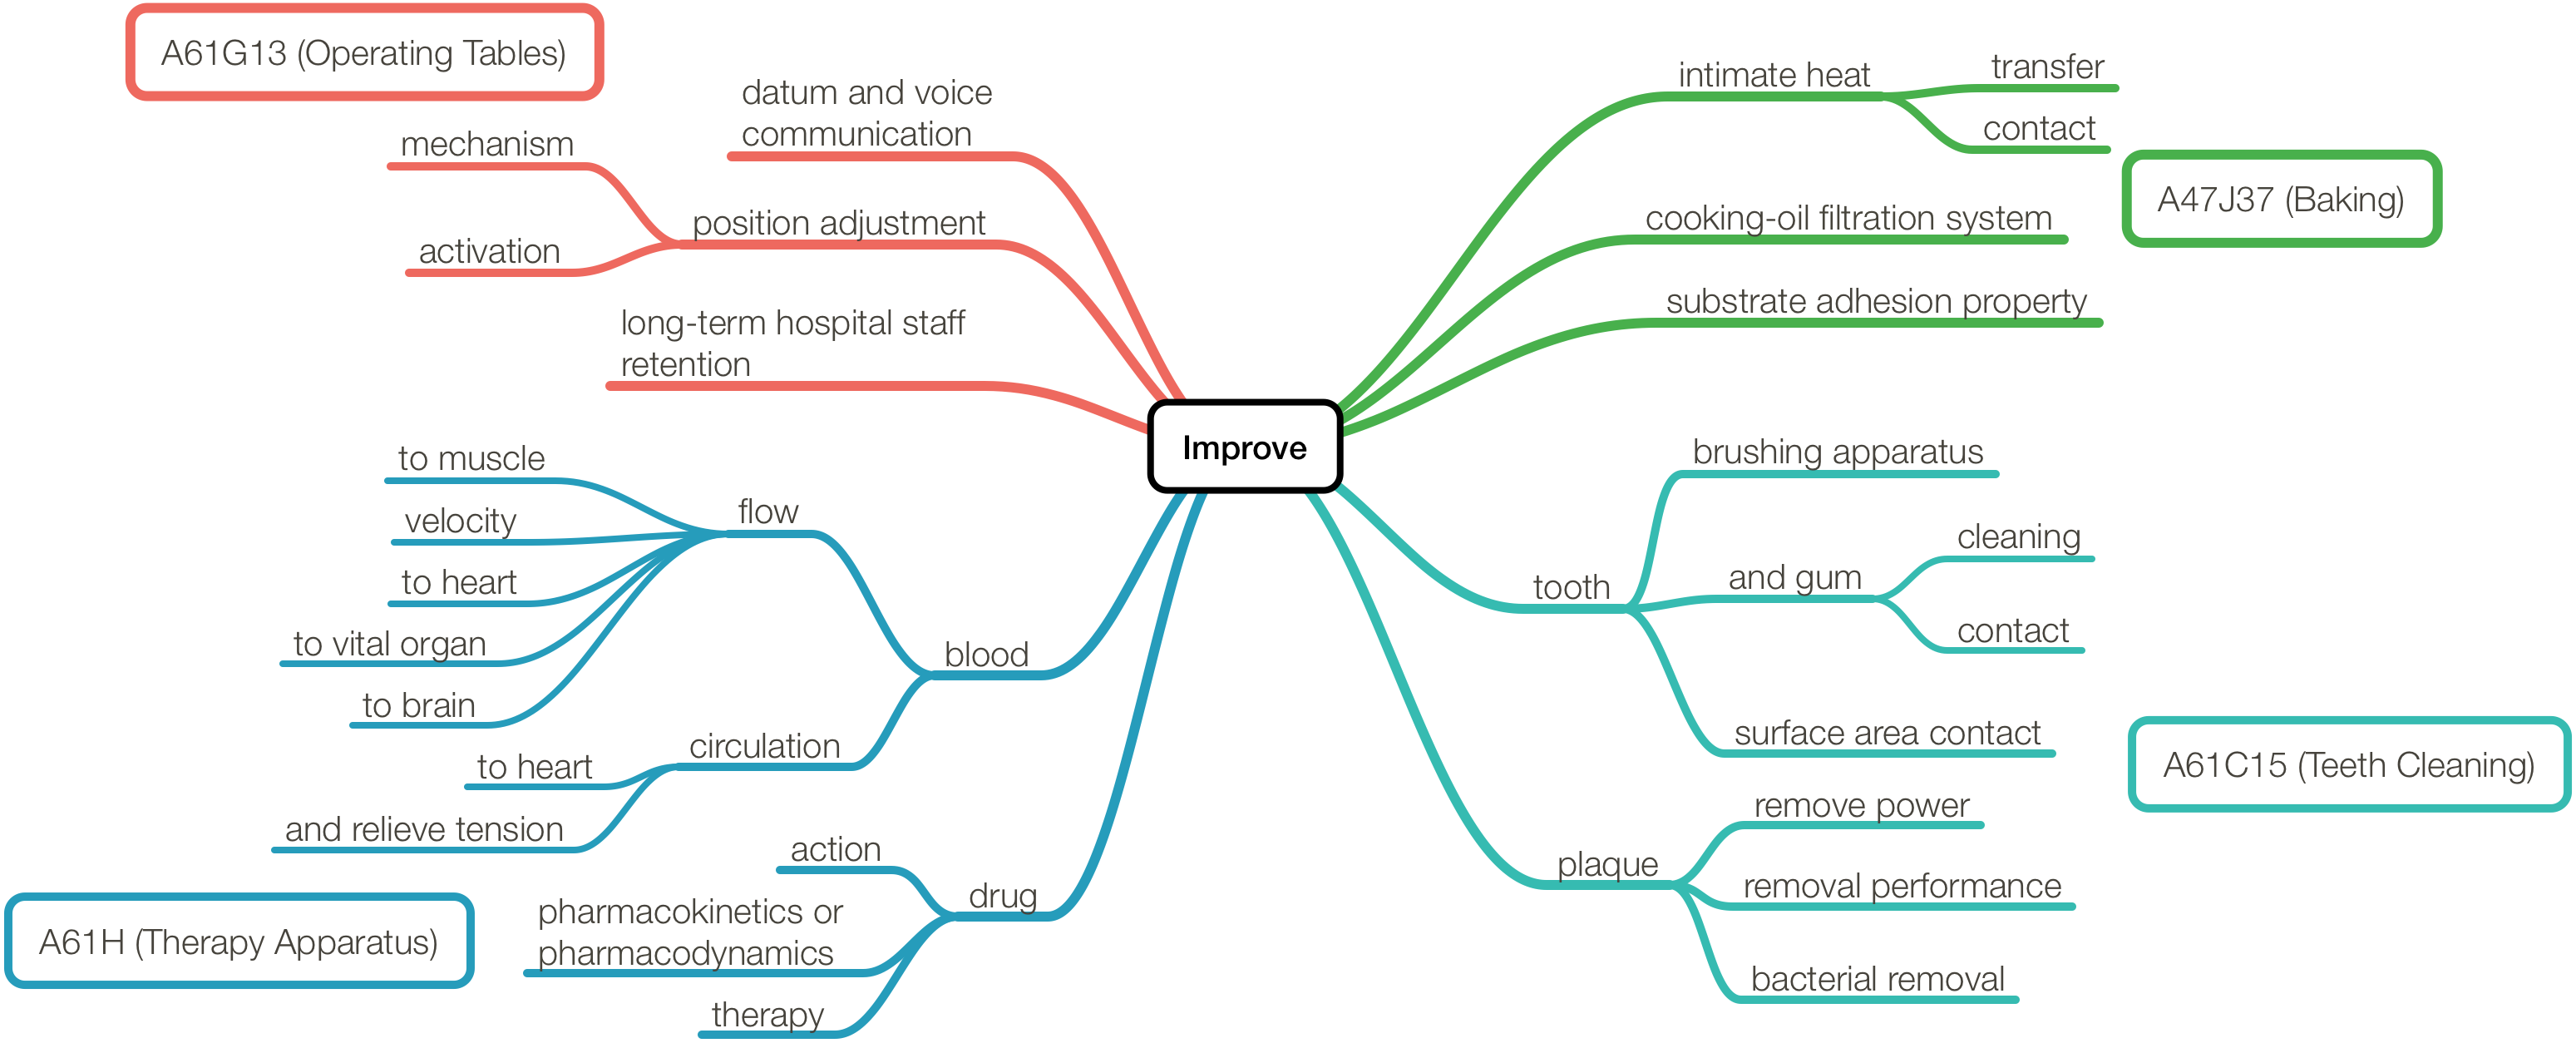
\includegraphics[width=1\linewidth]{_bookdown_files/figures/improve} 

}

\caption{Sample of the tree based taxonomy extracted from the analyzed patent sets. The sample contains some of the leaves linked to the advantage clue Improve}\label{fig:processimagetest1}
\end{figure}

\begin{figure}

{\centering 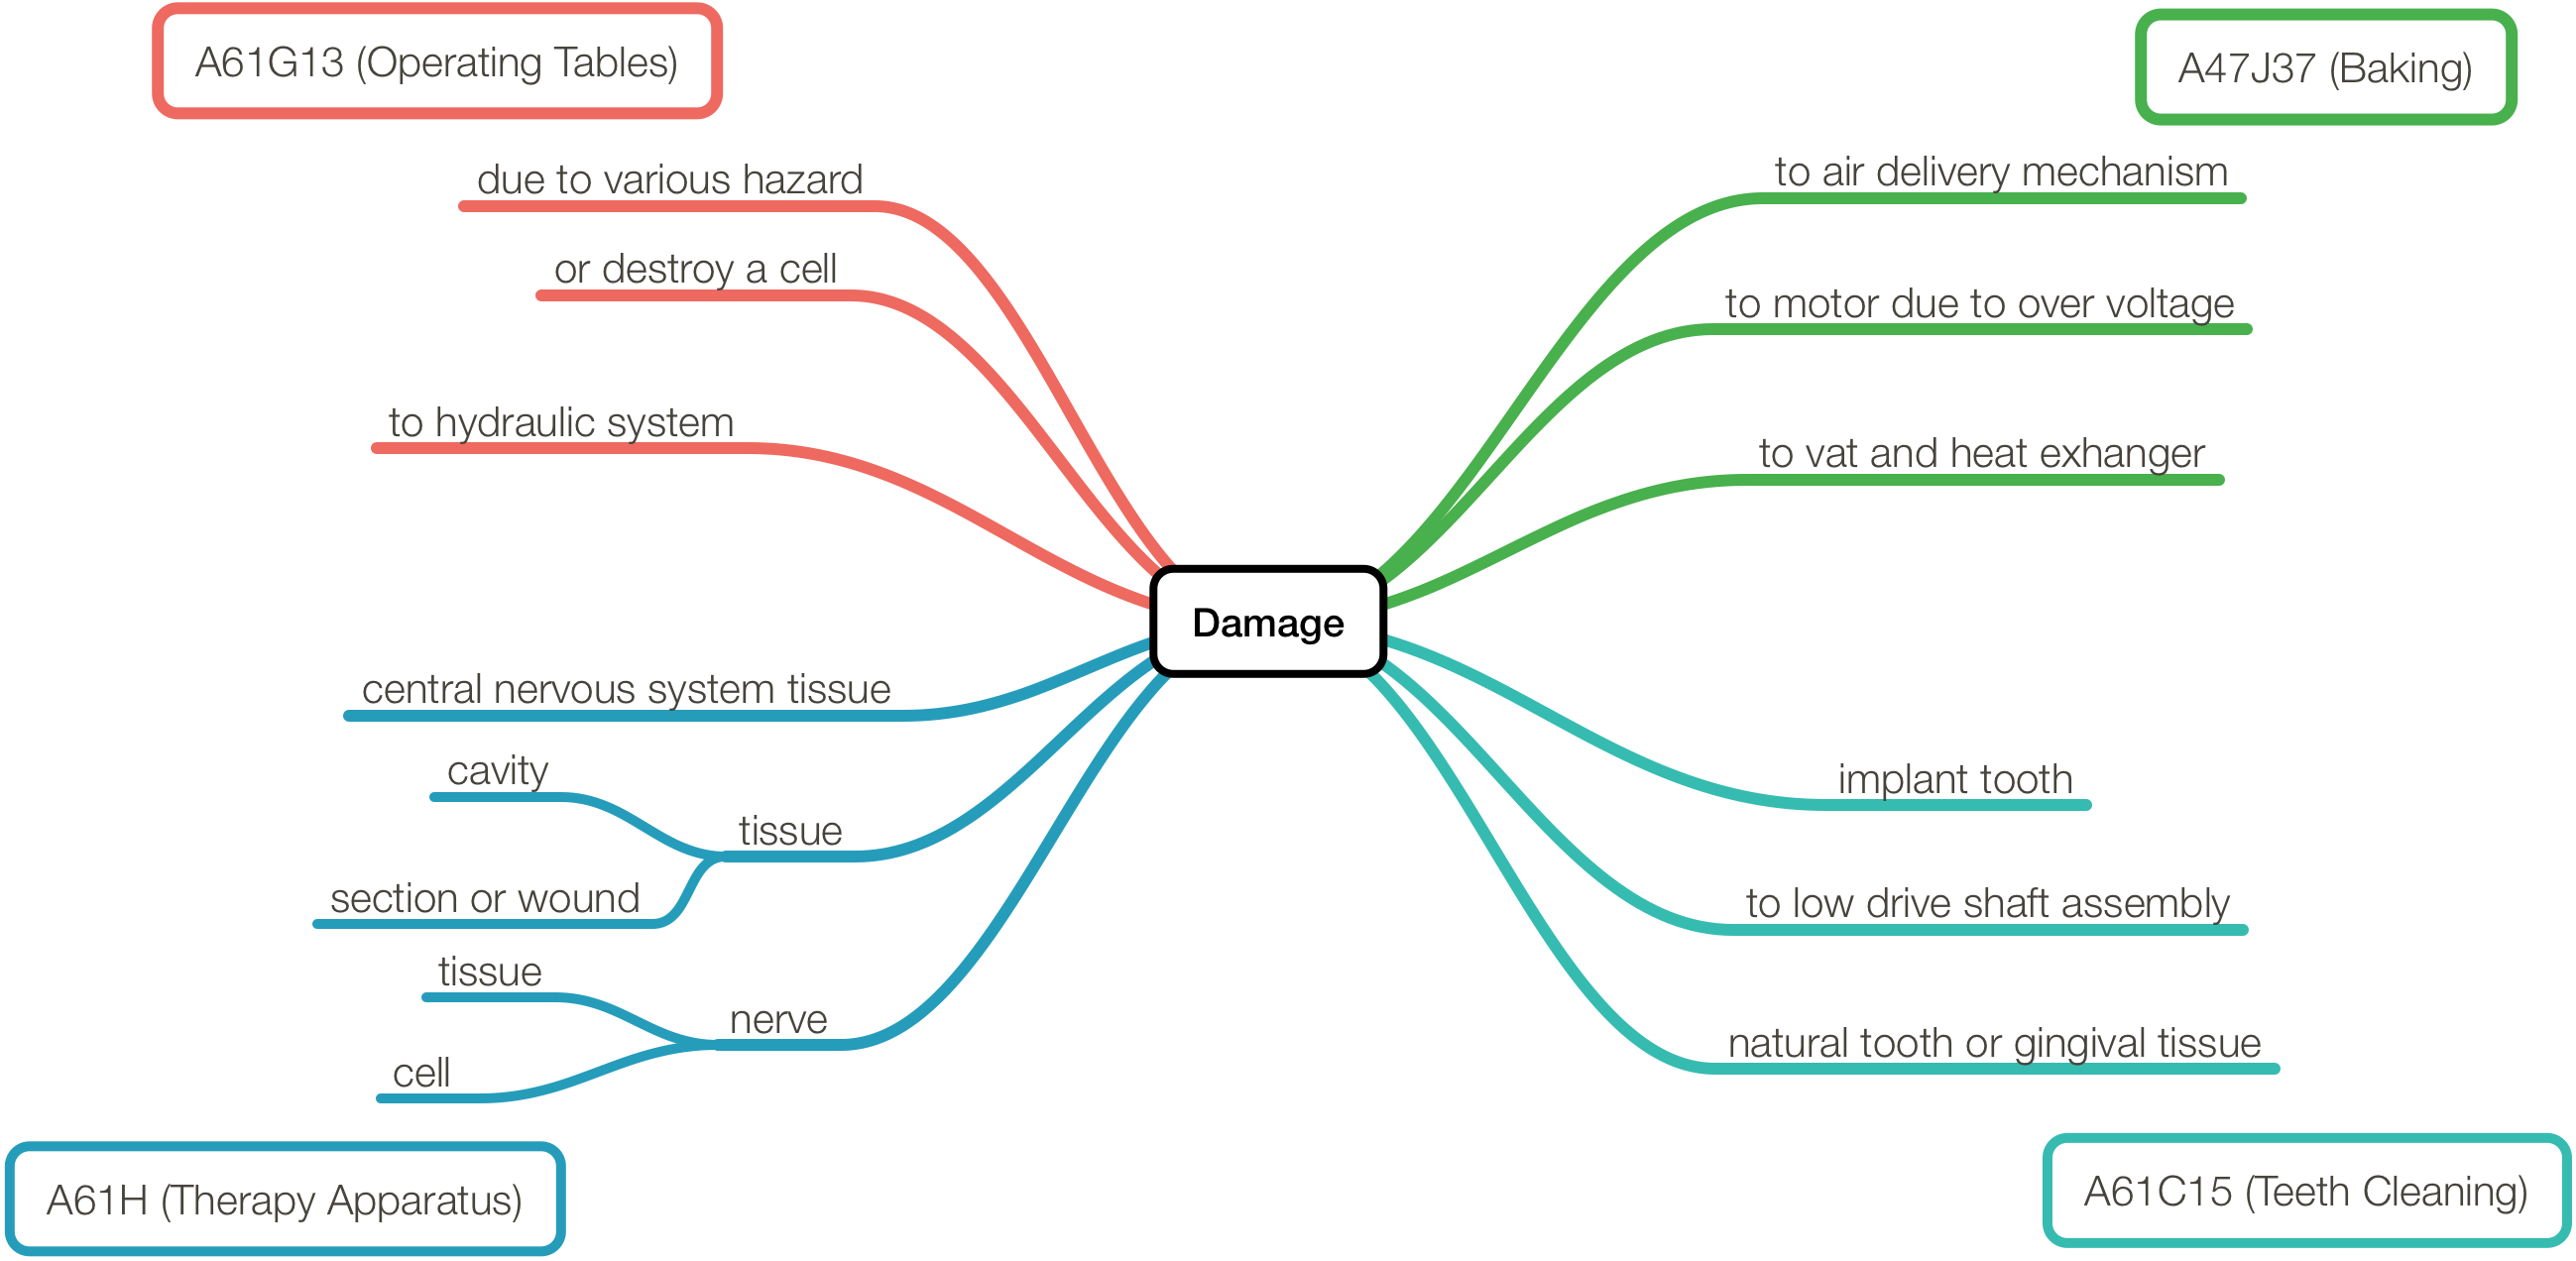
\includegraphics[width=1\linewidth]{_bookdown_files/figures/damage} 

}

\caption{Sample of the tree based taxonomy extracted from the analyzed patent sets. The sample contains some of the leaves linked to the drawback clue Damage. }\label{fig:processimagetest2}
\end{figure}

\section{Trademakrs}\label{trademakrs}

The market interest for both patents and trademarks has increased during
the last decades, with a significant increase in filing for both types
of Intellectual Property. The academia also took attention to patent
data and trademark data, but with different and (almost) disconnected
research approaches. Furthermore, the analysis of patents to study R\&D
is predominant while less attention has been paid to trademarks
\citep{griliches1981market}. Indeed, very few are the works where
patents and trademarks are investigated together and not generically
cited together as parts of the intellectual property right framework.
Moreover cultural differences exist between United States and Europe (at
least) and practical consequences can be observed in daily life: for
example, even if Europe had an earlier and more enduring interest in
trademarking than the US the presence of the symbols ® and ™ in the
product labels are more common in US than in Europe
\citep{mercer2010reading}. The difference exists also from an industrial
perspective, across different sectors \citep{baroncelli2004global}.
Indeed, trademarks have their larger use worldwide in the R\&D intensive
scientific equipment, pharmaceuticals sector and advertising intensive
manufacturing industries (clothing, footwear, detergents and food
products).

The present chapter studies the usage (if any) of \emph{trademarks} and
\emph{trade symbols} within patent texts. The aim is to investigate
possible indicators about IP strategies and innovation output utilizing
information about the interlink between patents and trademarks. An
additional goal is to understand if patent applicants makes a right use
of trademarks and trade symbols when writing a patent document. The
analysis clearly stands at the boundary between patent and trademark
research areas, and since such intermediate territory has not been
investigated in depth, there are several research questions we would
like to answer. The starting point is a sheer numerical evidence: we
have found out that, at the date of 01/09/2017, a total of 2.162.962
patents worldwide (for details about the database and its coverage see
section 3) contain a trademark symbol. It is therefore a not negligible
phenomenon, worth of investigation and that should provide interesting
insights about the mechanisms and strategies that companies adopt at the
frontier between technical innovation and marketing.

\subsubsection*{The use of trademark symbols ™ and ® in patents from a
legal
perspective}\label{the-use-of-trademark-symbols-and-in-patents-from-a-legal-perspective}
\addcontentsline{toc}{subsubsection}{The use of trademark symbols ™ and
® in patents from a legal perspective}

It is evident from our preliminary analysis that there exist an high
number of patent documents containing a trademark indication. In the
present section we investigate what is the legal perspective of this
usage.

In \citep{butler1969rules} the authors published a series of rules to
standardize the use of trade terms in patents. They also specifies
different rules in the case of use of trade terms in specifications and
the use of trade terms in patent claims. The rules are:

1- A trade term is properly used in a specification if those skilled in
the art can make the product designated by the trade term at the time
the application is filed, using the specification and/or published
literature that is implicated by the specification. 2- A trade term is
also properly used in a specification if the product is generally known
to persons skilled in the art and is readily obtainable at the time the
application is filed, provided the composition of the product is a trade
secret and there is reason to believe that whenever the composition of
the product is modified the trade term will also be changed. 3- A trade
term is also properly used in a specification if it designates a
component of the embodiment which is not essential to the invention. 4-
A trade term can be used in a claim only if its meaning has been
adequately defined in the specifications, whereby it imparts specific
limitations to the claim.''

The second rule is particularly interesting because it seems preventing
early patenting or patenting before having produced and used a trade
name. Rule number two is even more interesting since it contains a case
of a product that is a trade secret used to build another product
subject to patent application.

Similar guidelines are contained in the European patent convention
\citep{hall2018impact}. Here is state that is not desirable to use
trademarks or trade names if such words merely denote origin or where
they may relate to a range of different products. Anyway trademarks
could be used in patent application to satisfy art.83, that states that
the application shall disclose the invention in a manner sufficiently
clear and complete for it to be carried out by a person skilled in the
art. In this case the product must be sufficiently identified, without
reliance upon the word. A special case are such words that have become
internationally accepted as standard descriptive terms and have acquired
a precise meaning (e.g. ``Bowden'' cable, ``Belleville'' washer,
``Panhard'' rod, ``caterpillar'' belt). In this case they may be allowed
without further identification of the product to which they relate. It
is clear specifications afflicts the analysis that we want to carry out.
Always in the same document are given also guidelines for the usage of
trademarks in claims. These are, as expected, different from the
specifications. For claims we have the problem that it may not be
guaranteed that the product or feature referred to is not modified while
maintaining its name during the term of the patent. They may be allowed
exceptionally if their use is unavoidable and they are generally
recognised as having a precise meaning. It is the applicant's
responsibility then to ensure that registered trademarks are
acknowledged as such in the description. From that we can deduce that
the presence of a trademark in patents and more specifically in claims
decreases the reproducibility of the invention and thus the quality of
the patent. Also the the US patent legislation \citep{jaffe2000us}
focuses on the use of trademarks in patents claims. Here the presence of
a trademark or trade name in a claim is not considered improper but the
examiner should analyze the claim to determine how the mark or name is
used. In fact, the trademark or trade name should identify a source of
goods, and not the goods themselves. In this case the claim scope is
uncertain since the trademark or trade name cannot be used properly to
identify any particular material or product. In fact, the value of a
trademark would be lost to the extent that it became descriptive of a
product, rather than used as an identification of a source or origin of
a product. Thus, the use of a trademark or trade name in a claim to
identify or describe a material or product would not only render a claim
indefinite, but would also constitute an improper use of the trademark
or trade name.

Finally, in \citep{pressman2018nolo} the authors gives some guidelines
on how to introduce trademarks when it is unavoidable. First, the
trademark should be capitalized and used as an adjective (not a noun),
followed by the generic name of the product or service. Furthermore when
referring to the trademark there should also be a reference to the
trademark owner.

\subsection{Methodology}\label{methodology-1}

With respect to Users \ref{usersresults} and to Advantages and
Distadvantages \ref{advdrwresults} the process to extract tradenames
from patents is trivial. The main activity performed are (for details
aobut the activities see section \ref{sotatools}:

\begin{itemize}
\tightlist
\item
  Sentence splitting
\item
  Tokenization
\item
  Part-of-speech tagging
\item
  Lemmatization
\end{itemize}

After that is is possible to identify tradenames searching for the
symbols ™ and ®.

\subsection{Results}\label{results-2}

The first investigation has the aim of understanding if the ™ and ®
symbols has different content depending on different IPC \citep{wipo1}
classes. The IPC classes are: The main evidence in figure
\ref{fig:histtm} is that ® is used more than ™ in patent, with and
average percent of presence of 7.4\% and 5.6\% respectively. The reason
of this evidence could be that patents contains unregistered trademarks
that are never converted to registered trademarks; another reason is the
confusion between the ® and ™ symbol, usually considered as synonymous.
Furthermore the writer will use the symbol only if he/she knows that the
mark is protected, otherwise he/she will not indicate any symbols or
will use ™ or ® without checking the right use. Another possible problem
is that the word has become of common use and thus usually used without
symbols. Furthermore, classes A (Human Necessities) and C (Chemistry;
Metallurgy) clearly has more trade symbols than the other classes.

\begin{figure}

{\centering 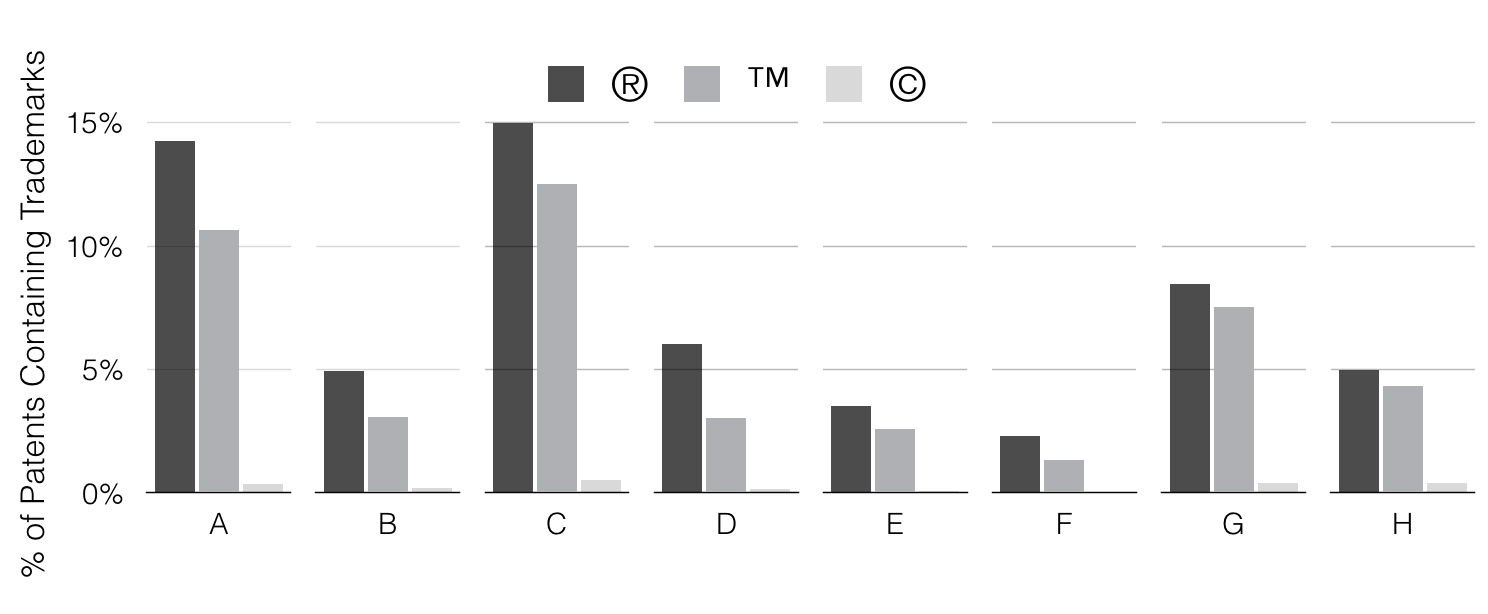
\includegraphics[width=0.8\linewidth]{_bookdown_files/figures/hist_tm} 

}

\caption{Histogram of the percentage of ® and ™ in patentes for each IPC class (limited to US patents). A (Human Necessities); B (Performing Operations; Transporting); C (Chemistry; Metallurgy); D (Textiles; Paper); E (Fixed Constructions); F (Mechanical Engineering; Lighting; Heating; Weapons; Blasting); G (Physics); H (Electricity).}\label{fig:histtm}
\end{figure}

Secondly, from table \ref{tab:ipcclassestm} it is evident that the
average ratio is 6.4 for ® (the usage is 6.4 times higher in the year
span 2007-2014 than the span 1995-2002) and 5.4 for ™ (the usage is 5.4
times higher in the year span 2007-2014 than the span 1995-2002) thus
the usage of trade-symbols in patent is growing and the presence of ® is
increasing faster than the presence of ™. From the present results is
not possible to say if this effect is due to an higher quality of the
process of patent application (and thus an higher awareness of applicant
and examiner) or of a positive trend in trademark registration. In
particular for the IPC class E (fields constructions) the number of ®
and ™ has increased 10.5 and 9.0 times respectively. This could be an
evidence of the fact that the number of trademark in the field of fixed
constructions is increasing.

\begin{longtable}[]{@{}lll@{}}
\caption{\label{tab:ipcclassestm} For each IPC class the ratio of the
percentage of patents containing at least one ® or ™ character is
computed for two patents sets 1995 to 2002 and from 2007 to
2014.}\tabularnewline
\toprule
\begin{minipage}[b]{0.13\columnwidth}\raggedright\strut
IPC Classes\strut
\end{minipage} & \begin{minipage}[b]{0.39\columnwidth}\raggedright\strut
Ratio ® 2007-2014 over ® 1995-2002 ~\strut
\end{minipage} & \begin{minipage}[b]{0.39\columnwidth}\raggedright\strut
Ratio ™ 2007-2014 over ™ 1995-2002 ~\strut
\end{minipage}\tabularnewline
\midrule
\endfirsthead
\toprule
\begin{minipage}[b]{0.13\columnwidth}\raggedright\strut
IPC Classes\strut
\end{minipage} & \begin{minipage}[b]{0.39\columnwidth}\raggedright\strut
Ratio ® 2007-2014 over ® 1995-2002 ~\strut
\end{minipage} & \begin{minipage}[b]{0.39\columnwidth}\raggedright\strut
Ratio ™ 2007-2014 over ™ 1995-2002 ~\strut
\end{minipage}\tabularnewline
\midrule
\endhead
\begin{minipage}[t]{0.13\columnwidth}\raggedright\strut
A\strut
\end{minipage} & \begin{minipage}[t]{0.39\columnwidth}\raggedright\strut
5.9\strut
\end{minipage} & \begin{minipage}[t]{0.39\columnwidth}\raggedright\strut
5.0\strut
\end{minipage}\tabularnewline
\begin{minipage}[t]{0.13\columnwidth}\raggedright\strut
B\strut
\end{minipage} & \begin{minipage}[t]{0.39\columnwidth}\raggedright\strut
6.2\strut
\end{minipage} & \begin{minipage}[t]{0.39\columnwidth}\raggedright\strut
5.4\strut
\end{minipage}\tabularnewline
\begin{minipage}[t]{0.13\columnwidth}\raggedright\strut
C\strut
\end{minipage} & \begin{minipage}[t]{0.39\columnwidth}\raggedright\strut
5.9\strut
\end{minipage} & \begin{minipage}[t]{0.39\columnwidth}\raggedright\strut
5.2\strut
\end{minipage}\tabularnewline
\begin{minipage}[t]{0.13\columnwidth}\raggedright\strut
D\strut
\end{minipage} & \begin{minipage}[t]{0.39\columnwidth}\raggedright\strut
5.6\strut
\end{minipage} & \begin{minipage}[t]{0.39\columnwidth}\raggedright\strut
5.7\strut
\end{minipage}\tabularnewline
\begin{minipage}[t]{0.13\columnwidth}\raggedright\strut
E\strut
\end{minipage} & \begin{minipage}[t]{0.39\columnwidth}\raggedright\strut
10.5\strut
\end{minipage} & \begin{minipage}[t]{0.39\columnwidth}\raggedright\strut
9.0\strut
\end{minipage}\tabularnewline
\begin{minipage}[t]{0.13\columnwidth}\raggedright\strut
F\strut
\end{minipage} & \begin{minipage}[t]{0.39\columnwidth}\raggedright\strut
7.5\strut
\end{minipage} & \begin{minipage}[t]{0.39\columnwidth}\raggedright\strut
6.2\strut
\end{minipage}\tabularnewline
\begin{minipage}[t]{0.13\columnwidth}\raggedright\strut
G\strut
\end{minipage} & \begin{minipage}[t]{0.39\columnwidth}\raggedright\strut
4.6\strut
\end{minipage} & \begin{minipage}[t]{0.39\columnwidth}\raggedright\strut
3.2\strut
\end{minipage}\tabularnewline
\begin{minipage}[t]{0.13\columnwidth}\raggedright\strut
H\strut
\end{minipage} & \begin{minipage}[t]{0.39\columnwidth}\raggedright\strut
5.1\strut
\end{minipage} & \begin{minipage}[t]{0.39\columnwidth}\raggedright\strut
3.2\strut
\end{minipage}\tabularnewline
\begin{minipage}[t]{0.13\columnwidth}\raggedright\strut
Average\strut
\end{minipage} & \begin{minipage}[t]{0.39\columnwidth}\raggedright\strut
6.4\strut
\end{minipage} & \begin{minipage}[t]{0.39\columnwidth}\raggedright\strut
5.4\strut
\end{minipage}\tabularnewline
\bottomrule
\end{longtable}

\subsubsection*{The Selected Tradenames}\label{the-selected-tradenames}
\addcontentsline{toc}{subsubsection}{The Selected Tradenames}

We a set of popular tradenames referring to
\citep{morris2016trademarks}. Then we filtered the ambiguous ones (the
one that can refer to surnames), because this can create an
overestimation of the number of patent citing it without the tradenames.
The total number of tradenames is 38 and these are: amazon®,
blackberry®, bose®, budweiser®, chiquita®, chrome®, cocacola®, ebay®,
facebook®, fender®, firefox®, gibson®, gillette®, heineken®, ibanez®,
intel®, iphone®, kellog®, kodak®, lego®, marlboro®, matlab®,
mcdonald's®, nitinol®, nutella®, nylon®, photoshop®, polaroid®, postit®,
powerpoint®, prozac®, sennheiser®, spotify®, teflon®, velcro®, whatsapp®
and xanax®.

In figure \ref{fig:tmlistcpmplete} are shown the number of patent
containing the tradenames with and without ™ and ®; furthermore the
information is divided for all the years, from 1995 to 2002 and from
2007 to 2014. In the previous analysis we noticed that ® is generally
more used than ™. Now the goal is to understand if patent writers uses
tradesymbols or not when citing tradenames, if there are any differences
between different tradenames and if we can notice different behaviors in
recent years. From figure \ref{fig:tmlistcpmplete} is evident that
despite the fact that it is mandatory to use ™ o ®, these symbols are
not always used.

\begin{figure}

{\centering 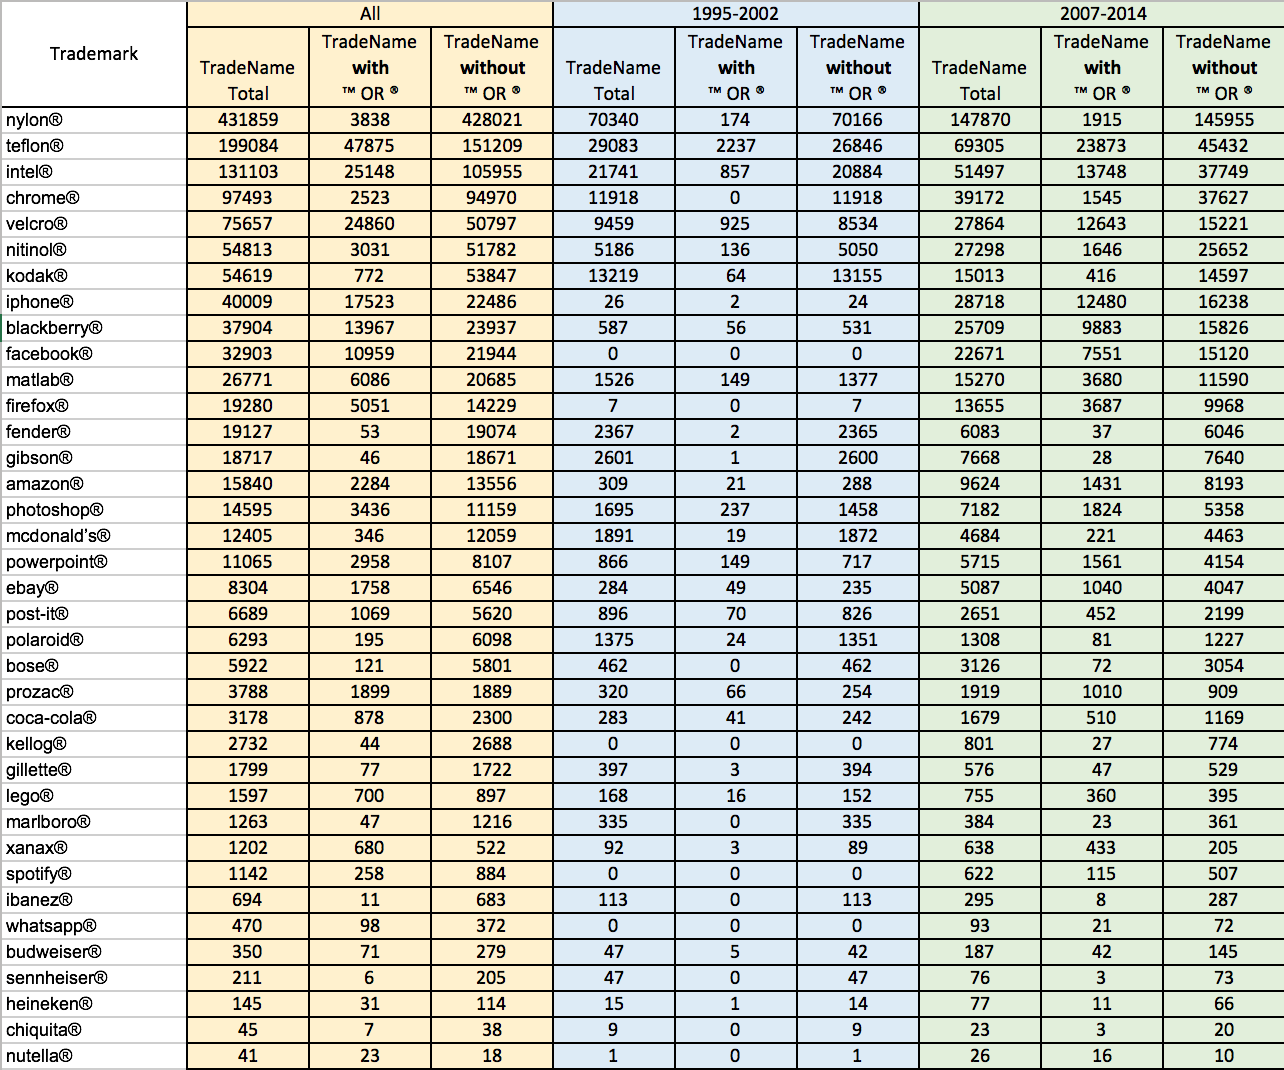
\includegraphics[width=1\linewidth]{_bookdown_files/figures/table_all_tradenames} 

}

\caption{Number of patents citing one of the 38 selected tradenames. The data are divided for any years, from 1995 to 2002 and from 2007 to 2014.}\label{fig:tmlistcpmplete}
\end{figure}

\subsubsection*{Tradenames Usage in
Patents}\label{tradenames-usage-in-patents}
\addcontentsline{toc}{subsubsection}{Tradenames Usage in Patents}

It is relevant to understand if there exists any difference between
different tradenames in the correct usage of trade symbols (a trade name
has been cited in the patent texts with the trade symbol). Figure
\ref{fig:tmcitedwell} illustrates in a bi-logarithmic plot the
distribution of trade names correctly cited in patents with ® and ™
(Y-axis) versus the same trade names cited without using the proper
symbol. Most of trade names are located under the diagonal. Those around
the diagonal are those we can considered as well known trademarks and
not so subject to genericization phenomena (green area). Conversely on
the right we can find a read area where the ratio is even more shifted
toward the absence of any indication of protected trademark. In the
middle the orange area where many of the most famous trademarks fall
down and that could be in phase of generalisation or conversely, since
the trademark of a product is totally entangled with the owner
(Iphone-Apple; Intel), inventors do not feel the reason to cite them as
a trademark. A remark on Figure \ref{fig:tmcitedwell} is necessary: the
plot presents a correct measurement of trademarks with ® and ™ plotted
in the y axis, while the search for trademark with missing trademark
symbols in some case can introduce undesired errors and include other
meaning of the word. Take for example the case of Blackberry®: the datum
is referring to mobile phones and accessories or software applications.
In all the cases where ® or ™ are correctly written, it is probably true
that the inventor is referring to the Blackberry® mobile phones, but
machines for jam or juice production extracted out of the blackberry
introduce false positive examples. Similarly Fender is probably located
too far on the right because it is also a part of a car, bike,
motorbike, boat, etc.. and Gibson could introduce citations of works
performed by someone called Gibson, therefore if cleaned results are
necessary the searching strategies for the trademarks without symbols
have to be refined.

\begin{figure}

{\centering 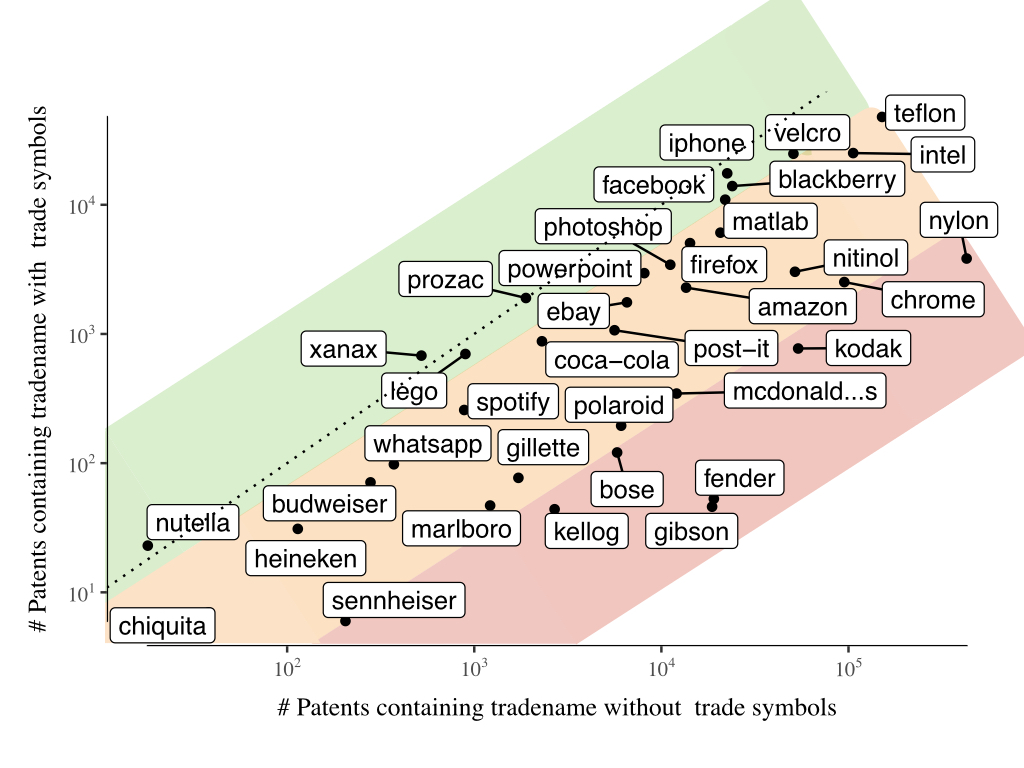
\includegraphics[width=1\linewidth]{_bookdown_files/figures/TrendsMarks.001} 

}

\caption{Plot of the trade names correctly cited in patents with ® and ™ on the y-axis and the same trade names cited without using the proper symbol on the x-axes. Both axes are on a logaritmic scale.}\label{fig:tmcitedwell}
\end{figure}

\subsubsection*{The Popularity of Tradenames in
Patents}\label{the-popularity-of-tradenames-in-patents}
\addcontentsline{toc}{subsubsection}{The Popularity of Tradenames in
Patents}

In figure \ref{fig:populartm} are plotted the trends of the numbers of
patents that correctly cite a tradenames. We analyzed 12 different
tradenames, divided in couples: each couple belong to a similar sector.
We make use of a generalized additive model fitting function to better
analyze the results and to make more easily to understand and compare
the two element of each pair.

Each pair has been chosen to compare trademarks in homogeneous markets.
Some of them shows:

\begin{itemize}
\item
  (d, e) similar trends but different incidence;
\item
  (a, c) dissimilar behaviors (Amazon vs Ebay, Blackberry vs.~Iphone:
  linear vs.~exponential);
\item
  \begin{enumerate}
  \def\labelenumi{(\alph{enumi})}
  \setcounter{enumi}{5}
  \tightlist
  \item
    similar results (e.g.~Gibson vs Fender in the music market have
    almost the same behavior and a reduced presence in patents)
  \end{enumerate}
\item
  similar behavior but shifted in time (e.g.~Firefox vs Chrome).
\end{itemize}

\begin{figure}

{\centering 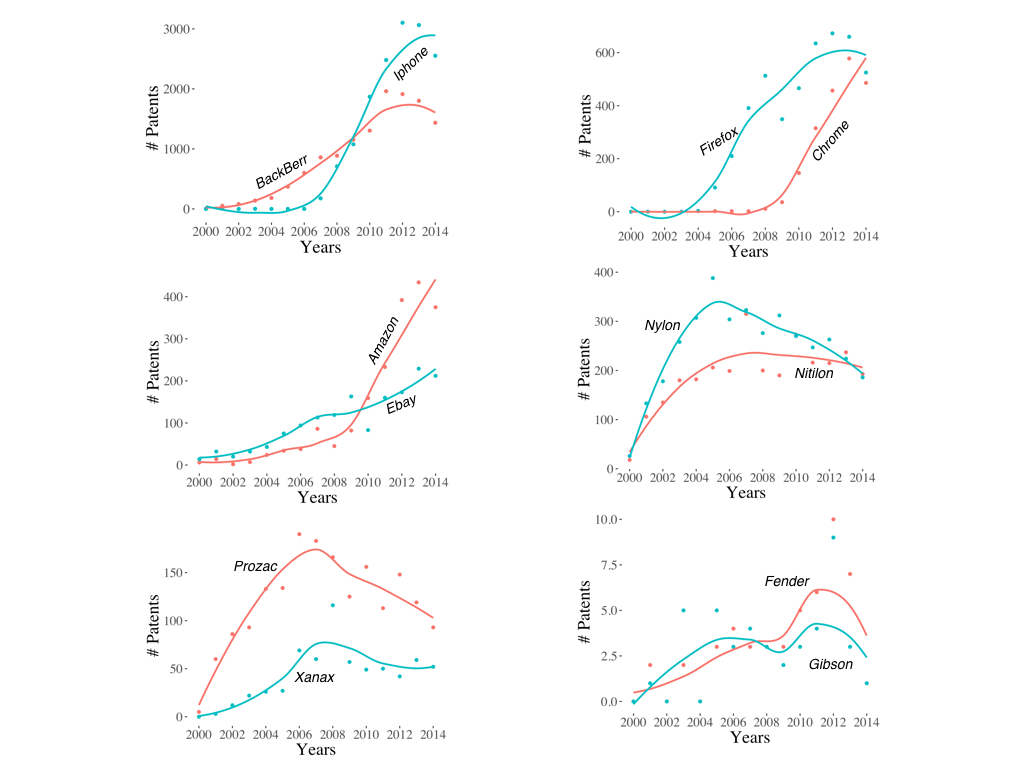
\includegraphics[width=0.8\linewidth]{_bookdown_files/figures/Marks_Years} 

}

\caption{Plot of the trade names correctly cited in patents from 2000 to 2014.}\label{fig:populartm}
\end{figure}

\subsubsection*{The Similarity of Tradenames in
Patents}\label{the-similarity-of-tradenames-in-patents}
\addcontentsline{toc}{subsubsection}{The Similarity of Tradenames in
Patents}

Further information can be derived by analysing the IPC classes where
the patent have been chosen by the assignees-attorneys-examiners.The
choice of a class is not only matter of market segment but rather of
market use. Moreover it is necessary to remark that from a formal point
of view the IPC classes form a feature vector, denoted y ∈ N639. IPC
classes form a complete dataset of 639 elements of such feature vector.
Each tradename is represented in such a feature vector where the number
of patents in each class constitutes the length of the vector along that
direction (feature). Our training data is therefore D = (x,y,z), where
x∈{[}1, .., 12{]}, y∈{[}1, .., 639{]}, and z represents the patent
numerosity z∈{[}0..15*106{]}. This dataset contains information about
how z varies as a function of x and y. The matrix is quite empty since
each product/brand addresses needs of specific market/s, after cleaning
of the totally empty columns the matrix reduces to the dimensions of
12x479 and demonstrates a correct choice of the trademarks since they
covered almost 75\% of the IPC space.

With such a dataset a series of computations can be performed: here we
show the results of the correlation analysis among the chosen trademarks
to analyse their relative positioning on the invention landscape (not
only the market); Correlation analysis is shown in Figure
\ref{fig:similartm}. The matrix is triangular owing to the symmetry of
the relationship.

\begin{figure}

{\centering 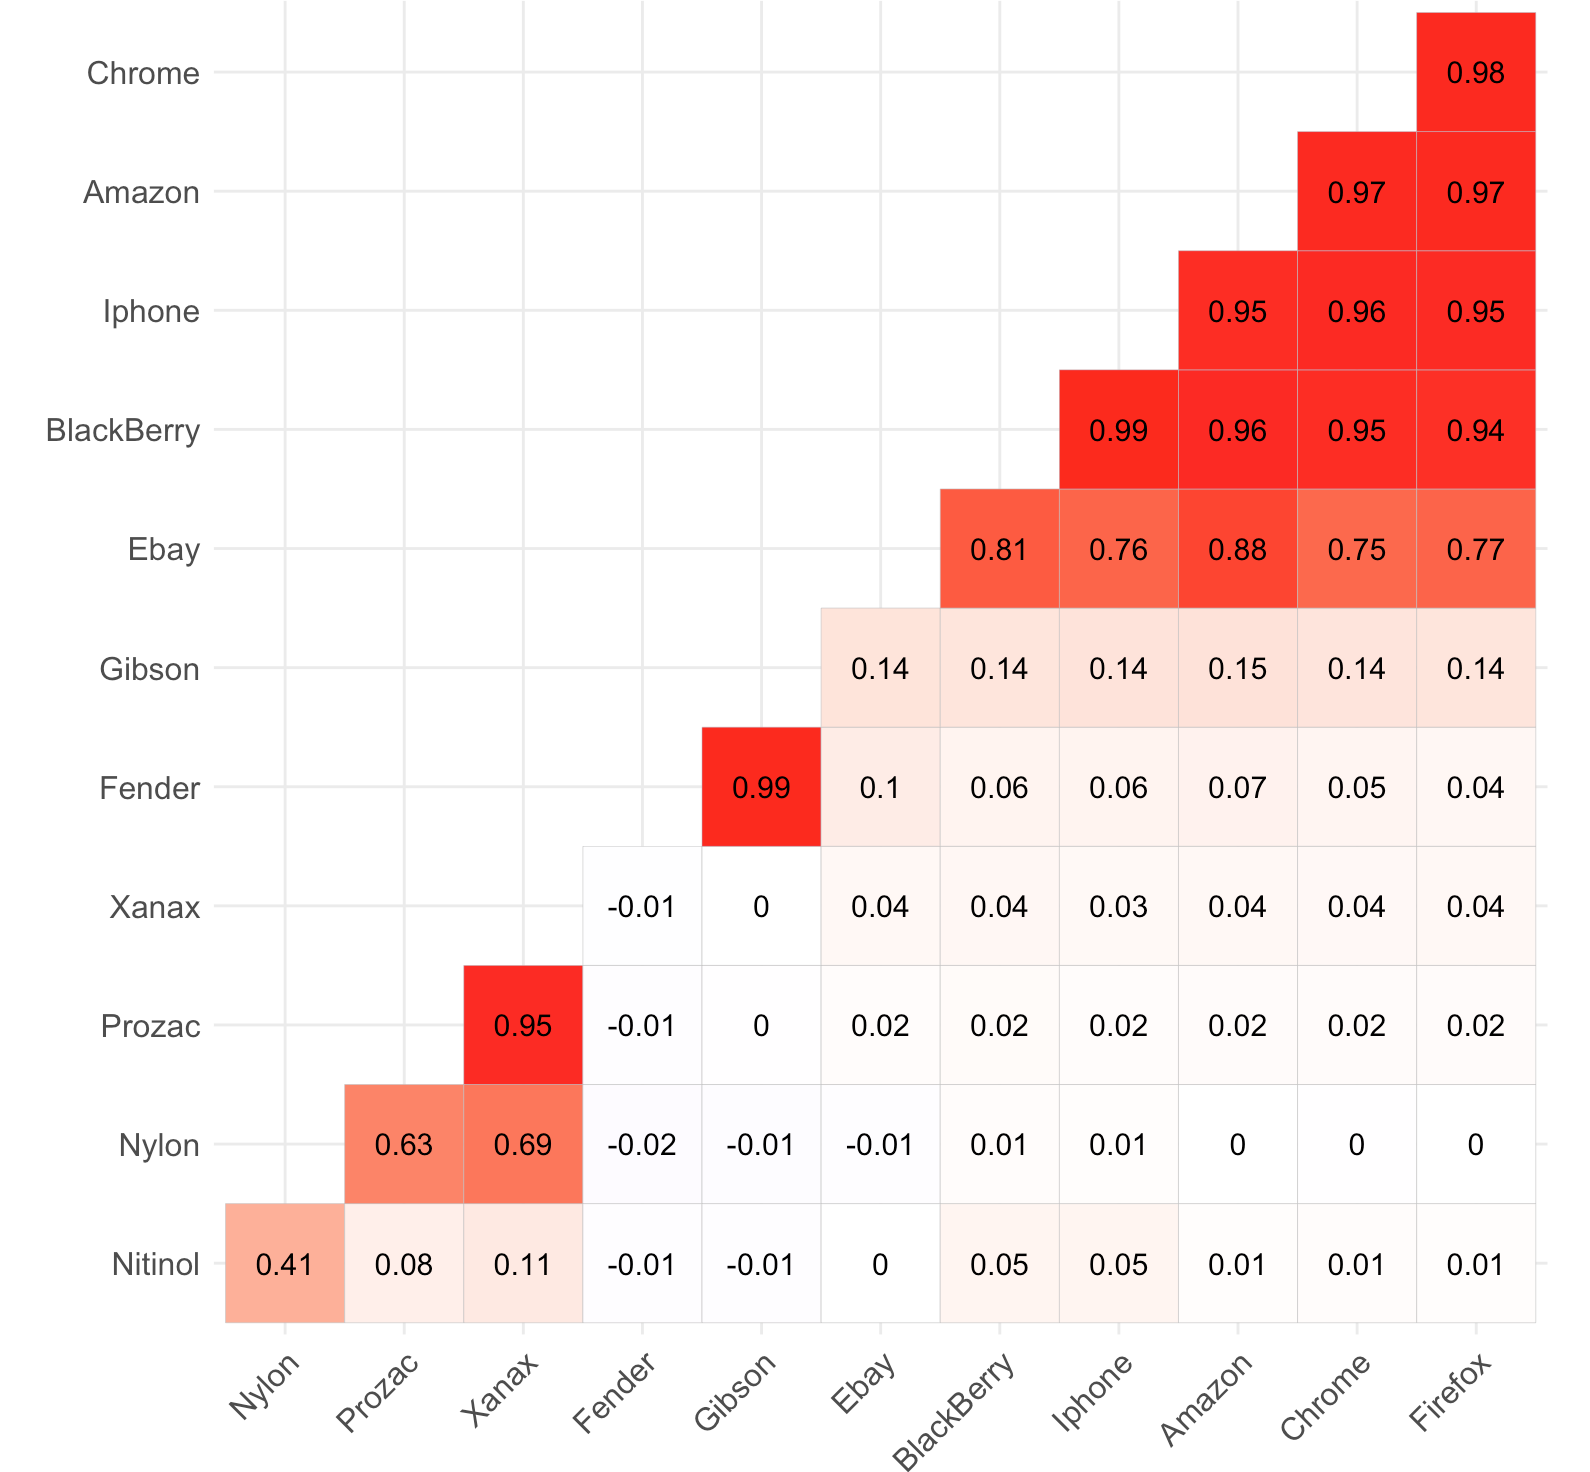
\includegraphics[width=0.7\linewidth]{_bookdown_files/figures/correlation_matrix_tm} 

}

\caption{Heat-map of the IPC-based similiraties between trademarks.}\label{fig:similartm}
\end{figure}

\chapter{Papers}\label{papers}

There are fields (mature technologies) where patents anticipate papers,
while in others (basic research) the opposite happens. For this reason,
scientific literature is the place where companies and scholars gather
information about the problems that researchers are facing in the
development of new technologies. Anyway, standard approaches of
knowledge extraction from papers requires skilled personnel, they are
time consuming and lacks in reproducibility. Furthermore, the volume of
scientific literature has grown rapidly raising an imminent question
about how to extract knowledge from this source. On the other hand, this
technical knowledge if managed, can be used to answer questions that 10
years ago would need the help of domain experts to be answered. In the
present section is shown how text mining techniques can help to answer
some of this questions. In particular, it is an essential problem when
different classification codes are used in order to organize scientific
knowledge on a specific domain, because a specific categorization in a
certain scientific field is missing. This leads to unnecessary
complications in the researchers' aims who want to quickly and easily
find literature on a specific topic among the large amount of scientific
publications, or want to effectively position a new research. Text
mining techniques, and in particular topic modelling, can help scholars
in solving this problems, if properly used together with domain
expertise. A deeper description of what patents are and how these
documents are used to mine technical knowledge can be found in section
\ref{sotadocumentspapers}

In this section we present two methodologies capable of automatically
segmenting a knowledge field. These selected knowledge field are:
sustainable manufacturing and block-chain. The results of the
methodologies are described, together with example of applications.

\section{Sustainable Manufacturing: the 6R
Framework}\label{smtextdrivenbottomup}

One of the most important objectives of Sustainable Manufacturing (SM)
is developing innovative and viable engineered materials, manufacturing
processes and systems to provide multiple life-cycle of products. In SM
the old concept ``from cradle to grave'' is now transforming into ``from
cradle to cradle'' \citep{jawahir2016technological}, tending toward
multiple product life-cycles or even a ``near-perpetual''
product/material life. Scientific contributions in the sustainable
manufacturing field mostly deals with energy and resource consumption.
In this respect, two different main fields of causes can be identified:
the process level and the material efficiency one. As a matter of facts,
manufacturing processes have a significant role also in putting in place
material efficiency strategies \citep{ingarao2017manufacturing}. As far
as the processes are concerned, a first classification of research
contributions was discussed in the CIRP General Assembly
\citep{duflou2012towards}. There the authors state that research in
manufacturing field, oriented to environmental impact reduction, can be
clustered in 5 main sub-classes:

\begin{enumerate}
\def\labelenumi{\arabic{enumi}.}
\tightlist
\item
  unit process level (Individual device or machine tool in the
  manufacturing system)
\item
  manufacturing system level,
\item
  facility,
\item
  multi-factory system up to considering the whole
\item
  supply chain level.
\end{enumerate}

Another review paper was presented at the ASME international
manufacturing science and engineering conference
\citep{haapala2013review}. In that paper the authors scrutinize the
research papers focusing more on the differentiation between
manufacturing processes and manufacturing system. Considering the
process level, Ingarao \citep{ingarao2017manufacturing} clustered the
scientific papers in 4 subsections: 1. effect of process parameters 2.
role of machine tool architecture and related technology 3. applied
process 4. manufacturing approach selection.

As concerns material efficiency options, a framework is presented by
\citep{allwood2014squaring}. The authors there provide strategies within
three main classes corresponding to principles: reduce, reuse and
recycling. Within each class guidelines for material efficiency
practices are detailed. As concerns material efficiency options, a
framework is presented by Allwood \citep{allwood2014squaring}. There the
authors provide strategies within three main classes (i.e.~principle):
reduce, reuse and recycling. Within each classes guideline for material
efficiency practices are detailed. A good framework of all the possible
reuses of materials is provided by Coopper \citep{cooper2012reusing}. In
this research the authors identify four main reuse strategies for
metals: Remanufacture, Reshape (applying metal shaping processes,
additive, subtractive, mass conserving) to obtain a new geometry,
Relocate: (recovering component and applying little refurbishment,
components reused in the same type of products), Cascade: recovering
component and use it in another less demanding use (downgrading). The
role of manufacturing processes in putting in place material
efficiency/reuse strategy was also outlined by Ingarao
\citep{ingarao2017manufacturing}. In fact, manufacturing processes
deserve to be considered as means for enabling material efficiency
strategies. SM may be pursued by several strategies, such as
re-designing and/or even changing manufacturing practices to conceive
new-generation products, as well as by creating a closed-loop of
environmentally-friendly material flow.

\subsubsection*{The 6R Framework}\label{the-6r-framework}
\addcontentsline{toc}{subsubsection}{The 6R Framework}

All the life-cycle stages of the product development (namely, design,
production, use and post-use) should be considered carefully, with a
particular attention to the design phase. This represents the real
difference introduced by sustainable manufacturing concept with respect
to traditional manufacturing, to lean manufacturing or even to green
manufacturing, precursors of the SM. In a word, SM paradigm embraces
those principles belonging to the 6R framework, namely: Reduce, Reuse,
Recycle, Recover, Redesign and Remanufacture. The latter three
principles where not included into the previous 3R framework. To a
certain extent, it appears that the better definition of sustainability
for any manufacturing operation provided so far is the extent to these
principles are applied. This statement justifies because in the search
to find a common rationale behind the mess of SM applications, one
possible way is to find common roots in the principles that inspired the
same applications: namely principles, which allows to the decision maker
either an effective way to search for new sustainable solutions or to a
certain extent measure the ``degree of sustainability''. The higher the
number of principles that are satisfied, the higher the potential
positive impact on sustainability can be for a given adopted solution.
In this sense, far from stating that the 6R framework is a widespread
and commonly adopted metric of SM, the starting assumption in this
section is that 6R is the only approach, to the author's knowledge, that
provides a criteria of classification and selection of solution, and
thus indirectly to provide a clear definition of what a SM application
may look like. The true question nowadays is \emph{if the 6R framework
may capture the essence of SM}, provided that it is really critical to
clearly define the SM paradigm rationale to the scientific community.
This section aims to stimulate the reflection from the Italian
perspective to this point, with a particular concern to the production
technology side, by using an automatic classification of papers within
the 6R framework and then by benchmarking approaches followed by the
Italian Technologist research-network SOSTNERE on SM issues.

Sustainability (from sustain plus ability) refers to the set of
properties of a given system (either natural or artificial), which
allows the same system to maintain itself for an almost indefinite
period of time. This concept was officially introduced in a document of
the World Commission on Environment and Development (WCED) entitled
``Our Common Future'', where the Sustainable Development was defined as
follows: \emph{``Sustainable development is development that meets the
needs of the present without compromising the ability of future
generations to meet their own needs''}\citep{wced1987world}. Starting
from this general definition, further conceptualizations have been
produced for manufacturing activities and/or processes, as here briefly
recalled. According to the Organization for Economic Co-operation and
Development, Sustainable manufacturing is a formal name for an exciting
new way of doing business and creating value. Different statements of
sustainability in literature \footnote{\url{http://www.trade.gov/green/sm-101-module.asp}}
share the same focus on the following three aspects: economy,
environment and society. It is thus possible to summarize from the
literature analyzed a possible definition for sustainable manufactured
processes/products, according to the following set of prescriptions:

\begin{itemize}
\tightlist
\item
  (-) minimize business risk;
\item
  (-) minimize negative environmental impacts;
\item
  (-) conserve energy and natural resources;
\item
  (-) are safe for employees, communities and consumers;\\
\item
  (-) are economically sound;
\item
  (+) a new way of creating value;
\item
  (+) are socially and creatively rewarding for all working people;
\item
  (+) providing access to basic services, green and decent jobs and a
  better quality of life for all ;
\item
  (+) adopt sustainable infrastructures.
\end{itemize}

where the (-) sign stands for those prescriptions oriented to
preservation of resources without any significant change of the present
condition, while the (+) sign indicates those prescriptions aiming at
ameliorating/modification of the trends with respect to traditionally
manufactured processes/products. To summarize simplifying, sustainable
manufacturing is all about minimizing business risks of any
manufacturing operation while maximizing the new opportunities that
arise from improving processes and products.\\
Fascinating in principle, these general statements are really difficult
to deploy into real operations and production settings. The focus of the
present analysis is to derive a clear definition of the concept of
manufacturing sustainability based on clear and paper based evidences,
rather than referring to general ethical or social principles, which
appear to be a \textbf{top down} definition. Conversely, information
extracted from all the scientific papers available on SM can provide a
sort of \textbf{bottom up} statement. Evidences are relevant words and
short concepts that can be related to sustainability, as it will be
explained in the following paragraphs by also providing some sound
examples from the Italian point of view.

\subsection{Methodology}\label{methodology-2}

In this section, we describe the process involved to analyse the papers
in the sustainable manufacturing field. To give a more detailed vision
of the topic, we consider this field divided in 6 sub-classes (one for
each principle), adopting the well know 6R framework. The goal of the
process is both to identify which the topics in each of the 6R are, then
to accurately measure the way this framework corresponds to the topics
of sustainable manufacturing. As seen in the flowchart of figure 1 the
main activities of the process are four: Paper manual classification,
Automatic Keywords Extraction, Keywords manual selection and Clustering.
Each activity will be described in the next subsection.

\subsubsection*{Assignment of 6R principle
meanings}\label{assignment-of-6r-principle-meanings}
\addcontentsline{toc}{subsubsection}{Assignment of 6R principle
meanings}

The first critical issue is the selection criteria of 6R principles for
the assignment. This was done by trying to assign a semantic
specification of each R principle, as below explicated, built by
summarizing all the possible definitions and concepts extracted by the
selected bibliography (partially cited in the present section). The
semantic specification provided below refers to the functional scope of
each class, intended as an activity to be performed.

\begin{figure}

{\centering 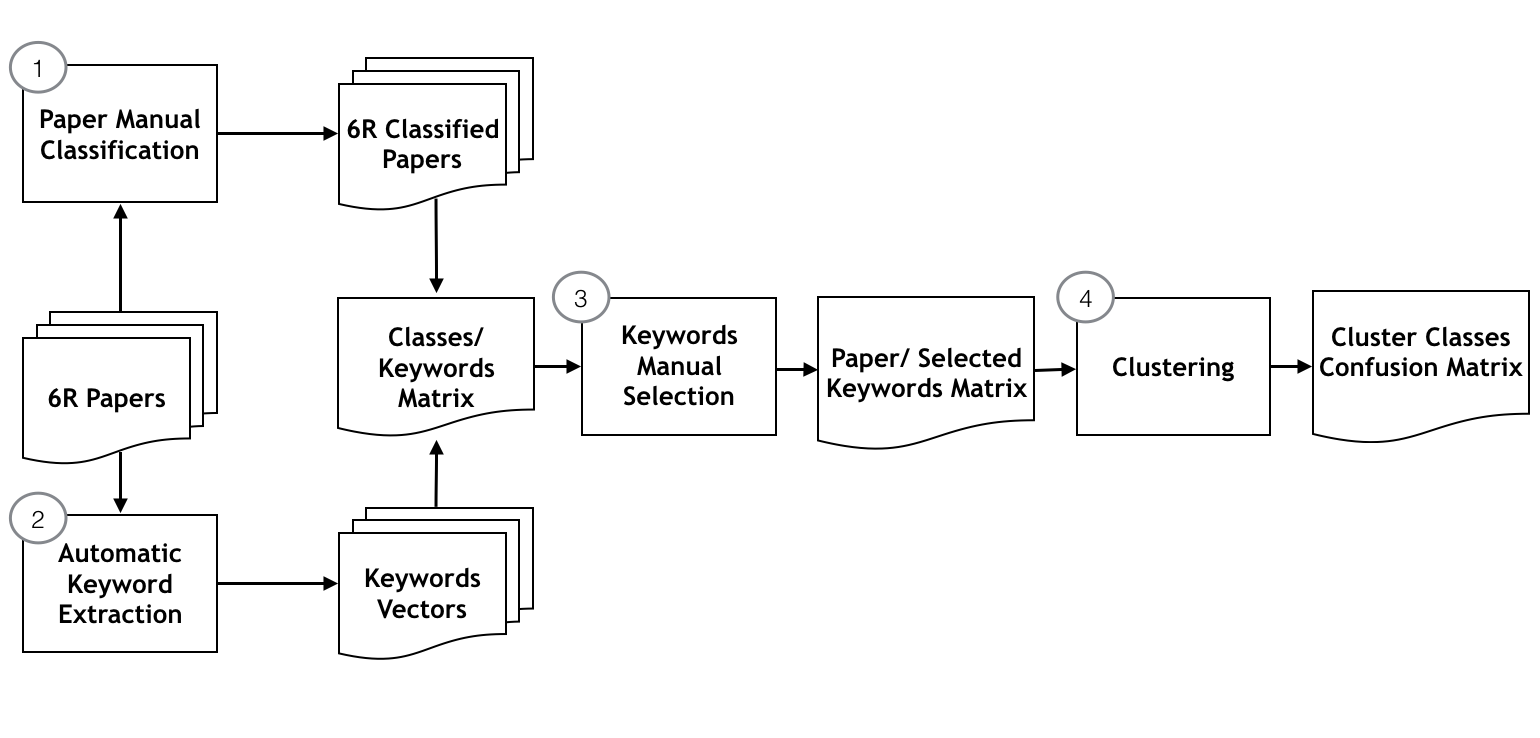
\includegraphics[width=0.8\linewidth]{_bookdown_files/figures/workflow_sm} 

}

\caption{Flowchart of the 6R papers analysis process. The white boxes represent the activities and the yellow boxes the predicted documents. In the figure are also highlighted the input and the main outputs of the process.}\label{fig:wfsm}
\end{figure}

\textbf{Reuse}

Reuse is the action or practice of using something again, whether for
its original purpose (conventional reuse) or to fulfill a different
function (creative reuse or repurposing). Reuse involves taking, but not
reprocessing, previously used items in order to save time, money,
energy, and resources. In particular reuse is useful for machineries,
especially when they are expensive, and for their components. Besides,
technologies can be also reused and re-adapted to different situations.
In addition, reuse is important because it minimizes disposal needs and
costs.

\textbf{Reduce}

In pre-manufacturing it is possible to implement the reduction
minimizing the use of resources. During the production phase, it refers
to the use of energy and material, for example, it may involve the use
of lower cost materials, the elimination of unnecessary product
characteristics, the reduction of overhead costs or the readjustment of
product processes. It implies a decrease of costs. As a consequence, the
derived effect of this principle is to minimize and optimize performance
in terms of cost, time and waste and it focuses primarily on the first
three stages of the four life cycle of the product before recalled.

\textbf{Recycle}

Recycle involves the process of converting material that would otherwise
be considered waste, into new products and it corresponds to the
breaking down of used items to make raw materials for the manufacture of
new goods. Recycling can prevent the waste of potentially useful
materials and reduce the consumption of fresh raw materials, thereby
decreasing: energy usage, air pollution (from incineration) and water
pollution (from landfilling). Recyclable materials include many kinds of
glass, paper and cardboard, metal, plastic, tires, textiles and
electronics.

\textbf{Recover}

Product recovery operations refer to operational processes
(e.g.~disassembling, sorting and cleaning) on products at the end of
their use, in order to make them usable in n subsequent life-cycles.
Differently from recycling, the product life-cycle is shortened,
skipping all that phases of retreatment of wastes up to their second
use. The risks of implementing product recovery operations is the
uncertainty of returned product quality and quantity and for this reason
recovering activities have only recently been considered in manufacture.

\textbf{Redesign}

The redesign activity involves the act of redesigning the next
generation of products, which would use components, materials and
resources recovered from the previous life-cycle or previous generation
of products. It refers to the evaluation of ideas turning them into
concrete innovative products obtained from products in their post-use
phase.

\textbf{Remanufacture}

Remanufacture involves the re-processing of used products, to restore
them to their original like-new state through the reuse of as many parts
as possible without loss of functionality. It includes and exceeds the
activity of recovering, because a remanufactured product should match
the same customer expectation as a new one.

Despite this initial classification, some problem occurred for experts
in assigning the papers to the different classes, due to the absence of
the formalization that is needed to define unique criteria of belonging.
This fact brought to the unbalance of the number of words within each
class (corresponding to each principle), that drove to the fuzziness of
the training set and, as a consequence, the difficulty in performing a
real classification of scientific papers. This is the first critical
issue of the followed approach so far, that may be overcome by alignment
sessions of the decision makers.

\subsubsection*{Automatic Text analysis and Keywords
extraction}\label{automatic-text-analysis-and-keywords-extraction}
\addcontentsline{toc}{subsubsection}{Automatic Text analysis and
Keywords extraction}

In order to analyze the information coming from scientific papers
belonging to topics encompassed within the 6R framework, we exploit text
mining techniques, which employ methods from different fields of data
mining to extract meaningful information 8. The second activity in our
analysis process is thus devoted to transforming the set of papers in a
set of numeric vectors to be elaborated by the clustering algorithm. To
this aim, some text mining techniques are applied in sequence 12 to
automatically extract meaningful information and knowledge from
unstructured texts. The text mining process performed is summarized in
the following. First, the information content of the document is
converted into a structured form (vector space representation). In fact,
most of text mining techniques are based on the idea that a document can
be faithfully represented by the set of words contained in it
(bag-of-words representation 9). According to this representation, each
document j of a collection of documents is represented as an
M-dimensional vector, where M is the number of words defined in the
document collection, and w(tji) specifies the weight of the word ti in
document j. The simplest weighting method assigns a binary value to
w(tji), thus indicating the absence or the presence of the word ti,
while other methods assign a real value to w(tji).

In the following, the text mining steps performed are described (for
details about the activities see section \ref{sotatools}:

\begin{itemize}
\tightlist
\item
  \emph{Tokenization} is the first step of our text mining process, and
  consists in transforming a string of characters into a string of
  processing units called tokens that could be syllables, words, or
  phrases. Typically, with tokenization other operations are performed
  with the aim of making the text cleaner. Such operations are the
  removal of punctuation and other non-text characters, and the
  normalization of symbols (e.g., accents, apostrophes, hyphens, tabs
  and spaces). In the proposed system, the tokenizer removes all
  punctuation marks and splits each text into tokens corresponding to
  words, bigrams and trigrams.
\item
  \emph{Stop-word filtering} consists in eliminating the words which
  provide little or no information to the text analysis, or that, in our
  case, could make the clustering process fuzzier. Common stop-words
  belong to certain part of speech classes, such as articles,
  conjunctions, prepositions, pronouns, etc. Other stop-words are those
  that typically appear very often in sentences of the considered
  language (language-specific stop-words), or in the set of texts being
  analysed (domain-specific stop-words). In our case, this second group
  consists of typical words of the scientific articles such as
  ``paper'', ``state-of-the-art'', ``present work''.
\item
  \emph{Stemming} is the process of reducing each word (i.e., token) to
  its root form. The purpose of this step is to group words with the
  same theme having closely related semantics. In the proposed system,
  the stemmer exploits the Snowball Stemmer for the English language,
  based on the Porter's algorithm.
\item
  \emph{Feature representation} consists in building, for each text, the
  corresponding vector of numeric features. Indeed, in order to cluster
  the texts, we have to represent them in the same feature space. In
  particular, we consider the F- dimensional set of features
  corresponding to the set of relevant stems.
\end{itemize}

\subsubsection*{Manual keywords
selection}\label{manual-keywords-selection}
\addcontentsline{toc}{subsubsection}{Manual keywords selection}

Keyword selection procedure was performed by hand from a team of 4
experts in the scientific field of sustainable manufacturing and with
consolidated expertise on research and innovation. In order to prevent
misunderstandings and difference in the judgement, a preliminary
analysis of the single attitudes to classification was statistically
performed and misalignment were eliminated by a guided training, based
on the contemporary evaluation of a same sample from different experts
so as to align the judgement. This process was done, as above mentioned,
based on the 6R explicit framework and sharing the meaning of each
principle.

It is clear that assignment of keywords to classes is not a trivial task
and susceptible of interpretation. Disambiguation process would be
required to explain the criteria of affinity to a given class, hopefully
by referring to the functional scope of each class. Still an ambiguity
may result, which can hardly be removed without a more profound
specification with appropriate examples, which is out of the scope of
the present paper.

According to this procedure the 6R refer to the following keywords:

\begin{itemize}
\tightlist
\item
  \emph{Recover}: recovery, planning processes, renewable resources, new
  approach, waste recovery; process scrap recovery; energy recovery;
  heat recovery; collection; separation; design for environment;
  material recover optimization; recovery logistics;
\item
  \emph{Recycle}: recycle, adhesive technologies, materials conversions,
  government regulation; (Advanced) recycling technologies;
  Recyclability; End of first life; Down cycle; New/Old process scraps;
  Material scraps; Landfill taxes; Recycling benefit awarding; Secondary
  material production; Embodied energy saving; Environmental legislation
\item
  \emph{Redesign}: machining, cutting, lubrication, environment
  technologies, cryogenic; Material-efficient design; Design for
  Environment; New Materials; Eco-friendly design; Eco-friendly
  materials; Material reduction; Light- weighting; Design for
  Disassembly
\item
  \emph{Reduce}: reduce, optimize, waste minimization, consumption,
  energy payback, pollution, reduction, emission, saving; Energy
  reduction; Waste reduction; Resource reduction; Material usage
  reduction; Process sustainability optimization; Energy efficiency;
  Heat efficiency; Manufacturing efficiency; Doing with less;
\item
  \emph{Remanufacturing}: remanufacturing, material processing,
  eco-efficiency, renewable, innovations, nanocomposites; Product
  renewal; Product upgrade; Reconditioning; Part replacement;
  Modularity; Disassembly; Inspection; Separation; Re-Assembly; Design
  for Remanufacturing
\item
  \emph{Reuse}: reuse, replacing, material flow analysis,
  eco-efficiency; Component reuse; product re-conditioning; product
  upgrade; non-destructive recycling; reuse supply chain; product
  maintenance; product repair; product monitoring;
\end{itemize}

It is clear that the keyword extraction is not a trivial task, since the
outcome of the process may range from a useless single word to a
meaningful group of combined words that, on the other hand, could become
too specific to be significant for the training set of the search
engines.

\subsubsection*{Paper Clustering}\label{paper-clustering}
\addcontentsline{toc}{subsubsection}{Paper Clustering}

Document clustering is the application of the general process of cluster
analysis to texts. The practical applications of document clustering
systems are several and vary from automatic document organization to
automatic topic extraction. For further details see section
\ref{sotatoolsmodelnetanal}. Independently from the kind of algorithm,
before the clustering phase, each document has to be represented as a
set of features. These features are typically the n-grams contained in
documents, so a critical activity for clustering effectiveness is the
n-grams extraction (or feature selection). This goal is achieved with a
series of sub-activity. These are typically tokenization (the process of
parsing text data into smaller units), stemming and lemmatization
(reducing all tokens to its semantic base), removing stop-words (less
important words), and finally computing term frequencies (or other
measures of the relationship between documents and words).

To get an exploratory view of the degree of precision with which the 6R
framework represents the papers in analysis, the manually classified
documents were clustered using a clustering Spherical K-Means Clustering
algorithm \citep{buchta2012spherical}. We will then compare the output
of the algorithm with the manual classification in the following
paragraph.

Spherical k-means exploit cosine dissimilarities to perform
prototype-based partitioning of term weight representations of the
documents. Prototypes are centroids defined in the same feature space of
the documents. The aim of the algorithm is to minimize, given a set of
objects (documents in our case) and prototypes described in the same
features space (the selected keywords) the cosine distance between each
element and the closest prototype. This implies that the output of the
algorithm is a membership matrix, in which each document is assigned to
a certain prototype.

\subsection{Results}\label{results-3}

In the present section, we describe the output of the application of the
methodology on the 339 selected scientific papers on sustainable
manufacturing extracted by the query ``sustainable manufacturing'' in
the paper search field of the SCOPUS® database. Accordingly, apart the
deliberate selection of the source database, no other filter was applied
in the journal selection and this guarantees the significance of the
journal sample selected. The main output, as highlighted in Figure 1, is
the distribution of documents among the 6R principles (i.e.~classes) as
manually classified, the automatic keywords representations of the
classes and the outputs of the clustering algorithm (which is an
unsupervised assignment of the documents) compared to the manual
classification.

The assignment of a paper to a class was made by recognizing the
application, or tools or scope of the paper to one 6R's principles. In
this sense, for instance, a paper belonging to a recover might have as
scope, or keywords or approach or an activity performed with the
principal task to assure the recovery of a give good. It is thus clear,
from the beginning, how complex may be to recognize just one principle
more than a multiple possibility to satisfy more principles. This fact
will be discussed in the followings.

\subsubsection*{Distributions of documents among the
6R}\label{distributions-of-documents-among-the-6r}
\addcontentsline{toc}{subsubsection}{Distributions of documents among
the 6R}

The main point coming out from the histogram in Figure
\ref{fig:smhistogram} is that the distribution of scientific papers
assigned to the 6R principles (classes) is not homogeneous. If the four
classes Reduce, Recycle, Redesign and Remanufacture collect a comparable
number of papers, the other two (Reuse, Recover) are poorly represented.
One possible explanation of this is that cases of reuses or recoveries
are less generalizable compared to other ``R'', and thus potentially
less interesting for conferences and journals. Recovery and reuse, in
fact, often refers to specific functions embedded into the product, and
finding a general rule for assessing or designing such processes might
be more difficult. They rather might find room in technical magazines,
not included in the present analysis as concern processes. It worth
noting that reuse and recover here refers to product and not explicitly
to materials. Different approach concerns the design for reuse, which to
a certain extent would belong to remanufacturing, as in the most of
papers discussed, to mention a few, in the Annals of CIRP 18,19,20. It
is difficult to think that the classification criteria, which plays a
critical role into the assignment to classes, contributed to this
situation, depending on the meaning assigned to each principle. Whether
a different combination of classed have been provided, a different
histogram would be expected to appear.

\begin{figure}

{\centering 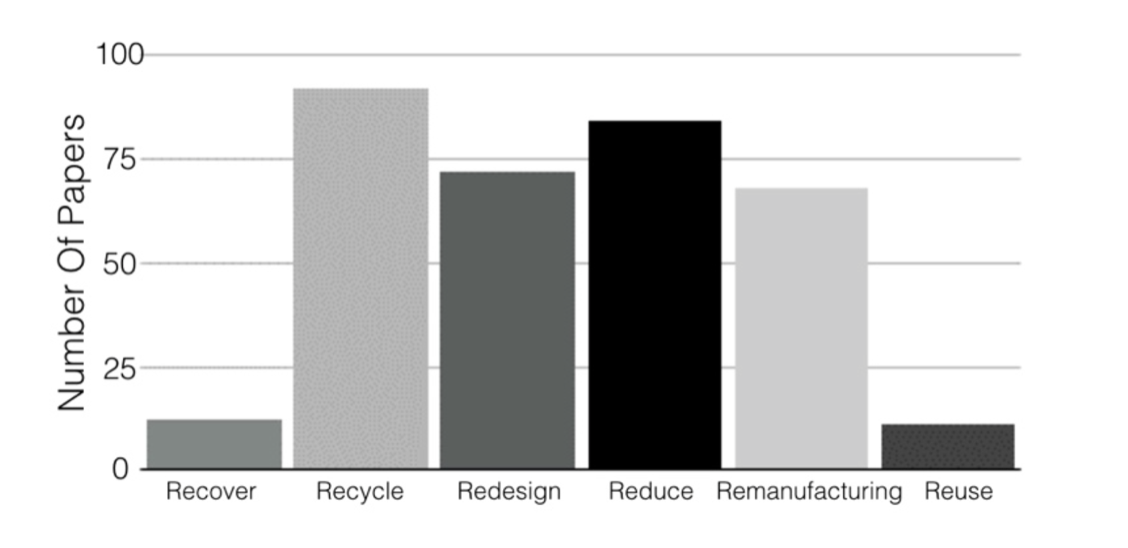
\includegraphics[width=0.8\linewidth]{_bookdown_files/figures/sm_histogram} 

}

\caption{Histogram of the number of papers manually assigned to each of the 6R principles.}\label{fig:smhistogram}
\end{figure}

\subsubsection*{Keyword vector representation of
6R}\label{keyword-vector-representation-of-6r}
\addcontentsline{toc}{subsubsection}{Keyword vector representation of
6R}

After the phases of automatic keyword extraction and manual keyword
selection, we derived the paper/selected keywords matrix. A sample of
the elements of this matrix (keyword and their occurrency) is:

\begin{itemize}
\tightlist
\item
  \emph{Recover}: Life cycle 5, environmental impact 4, raw material 3,
  cycle assessement 3, tossii fuel 3, energy payback 2, cleaner products
  2, energy cost 2, energy usage 2, pv System 2, product process 2,
  managements System 2, new technologies 2, energy save 2, climate
  change 2, risk assessements 2
\item
  \emph{Recycle}:lite cycle 40, environmental impact 31, waste
  management 30, resource conservation recycle 25, solid waste 21, lite
  cycle assessement 18, recycle material 14, recycle process 12, reuse
  recycle 11, electronic equipement 11, global warm 9, waste disposai 9,
  heavy metal 8, environment friendly 8, waste treatment 8, waste stream
  8
\item
  \emph{Redesign}: manufacturing process 20, lite cycle assess 19,
  sustainable manufacturing 17, machine tool 14, naturai gas 14, cutting
  tool 13, raw material 13, tool life 13, cutting fluid 13, tool wear
  13, mechanical engineering 12, System boundaries 11, machining process
  11, manufacturing System 11, cutting speed 11, cutting zone 10
\item
  \emph{Reduce}: life cycle 40, environment impact 38, energy
  consumption 31, life cycle assessment 28, energy usage 22, energy
  requirements 18, solar energy 15, cleaner product 13, global warm 13,
  climate changes 12, solid waste 12, gas emission 11, solar celi 11,
  cutting conditions 11, co2 emissions 10, environmental management 10
\item
  \emph{Remanufacturing}: sustainable manufacturing 28, manufacturing
  process 22, remanufacture product 18, supply chain 16, new product
  development 16, climate change 12, business model 12, product
  remanufacturing 12, manufacturing System 11, environmental
  performances 10, remanufacturing industry 10, management System 9,
  waste generation 9, design for environment 9, remanufacture and
  recycle 8, automotive industry 7
\item
  \emph{Reuse}: life cycle 7, environment impact 7, energy usage 4,
  mechanical engineering 4, industriai ecology 4, cleaner product 3,
  life cycle assessement 3, environment management 3, design for
  manufacturing 3, environment protection agency 3, waste management 3,
  united nation 3, environment management System 2, process design 2,
  sustainable manufacturing 2, green chemistry 2
\end{itemize}

The keywords were divided according to the 6R principles (i.e.~class),
listing the number of the paper belonging to each class.The sample list
of keywords and their occurrency, reflects the distribution of figure
\ref{fig:smhistogram} and cannot thus be significant for classification
but only for clustering purposes at the present.

\subsubsection*{Clusters/classes confusion
matrix}\label{clustersclasses-confusion-matrix}
\addcontentsline{toc}{subsubsection}{Clusters/classes confusion matrix}

To analyze from a semantic dimension how well 6R framework represent
sustainable manufacturing definition through the scientific papers
considered, the manually classified documents were clustered using a
clustering Spherical K-Means Clustering algorithm. The results (the
assignments of each paper to a cluster) was then compared with the
manual classification. The number of resulted clusters was 6, having
this number of clusters no specific relation with the number of 6R
classes. The output of the clustering process is thus a 6x6 Matrix
(Class(row)/Cluster (column)) shown in Figure \ref{fig:clusterssm}.
Numbers in the cells of the matrix represents centroids that can be
characterized by the related keywords.

\begin{figure}

{\centering 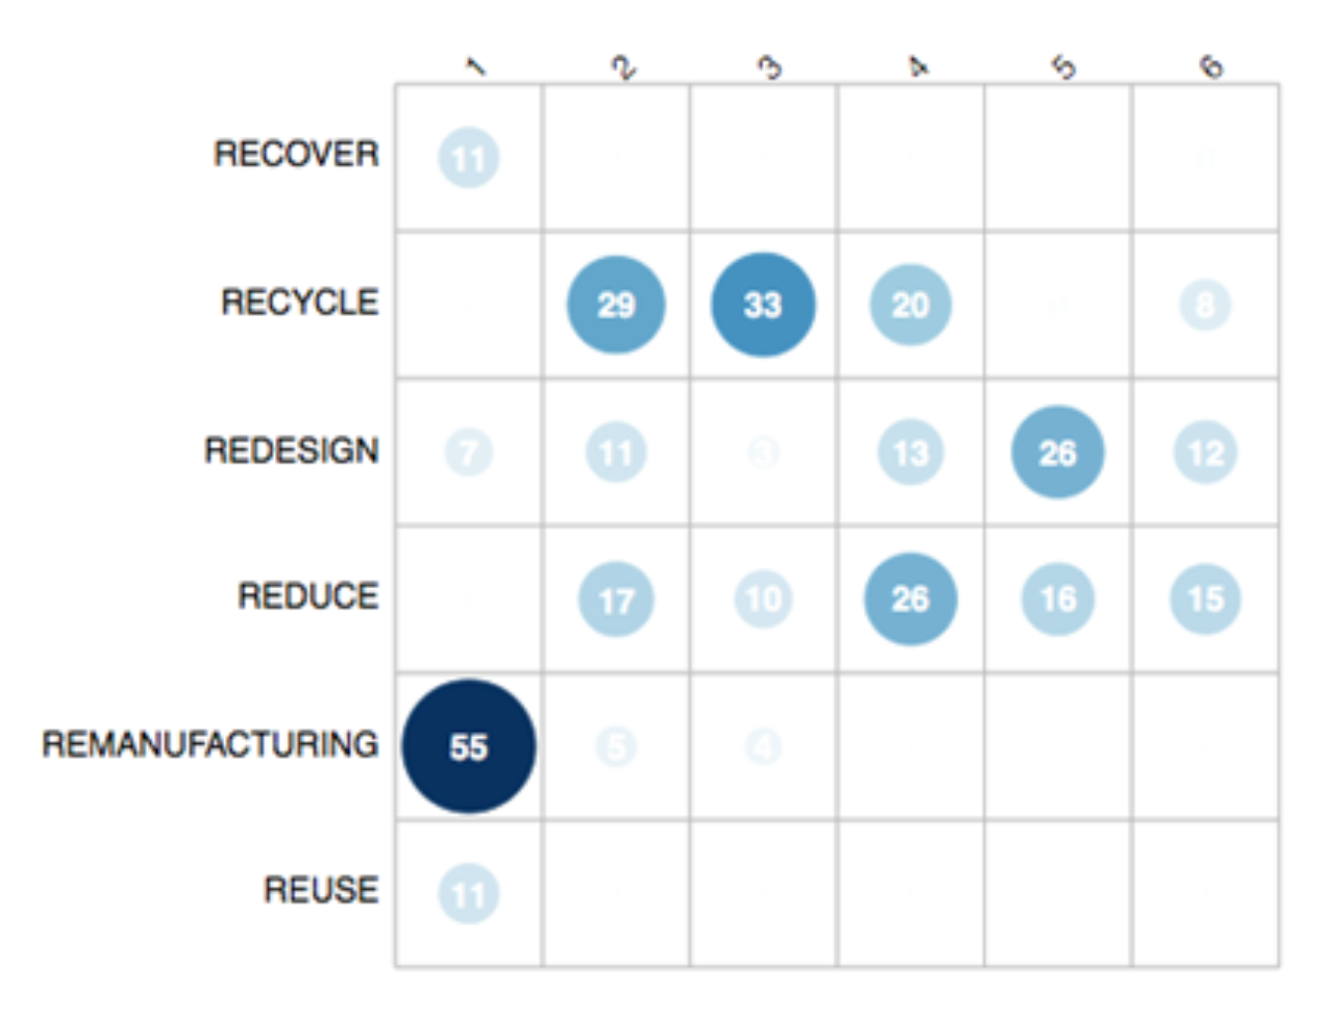
\includegraphics[width=0.6\linewidth]{_bookdown_files/figures/heat_map_sm} 

}

\caption{Matrix: comparing the manual classification and the clustering output.}\label{fig:clusterssm}
\end{figure}

\section{Sustainable Manufacturing: An Extended
Mapping}\label{sustainable-manufacturing-an-extended-mapping}

The methodology described in section \ref{smtextdrivenbottomup} has been
then re-adapted to give an extended analysis of the 6R framework from a
bottom-up perspective. In the present section, we map the state of the
art of Sustainable Manufacturing using topic modelling, a widely used
text mining techniques. The aim is to give a broad overview of how this
knowledge field is approached world-wide and then, in section 3, to have
a deeper look at the Italian way to sustainable manufacturing.

\subsection{Methodology}\label{methodology-3}

The process of topic extraction is composed by the subsequent
activities:

\begin{enumerate}
\def\labelenumi{\arabic{enumi}.}
\tightlist
\item
  \emph{Papers Collection}
\item
  \emph{Keyword Extraction}
\item
  \emph{Topic Modelling:} Number of topic selection
\item
  \emph{Topic Modelling:} LDA Model fitting
\item
  \emph{Manual topic labelling}
\end{enumerate}

Each activity is described in the subsequent sections.

\subsubsection*{Papers collection}\label{papers-collection}
\addcontentsline{toc}{subsubsection}{Papers collection}

The analysis starts form a corpus of papers on sustainable
manufacturing. The papers were downloaded from the Scopus database
searching for the query:

\begin{equation*} 
  TITLE-ABS-KEY("sustainable.*manufacturing")
\end{equation*}

At the date of 29/05/2018 the query results in 1,628 documents.

\subsubsection*{Keyword extraction}\label{keyword-extraction}
\addcontentsline{toc}{subsubsection}{Keyword extraction}

We represent each article as a set of keywords, merging Author Keywords
and Index Keywords. The keywords are then ``sanitized'' following the
subsequent rules:

\begin{itemize}
\tightlist
\item
  Eliminate duplicated keywords
\item
  Eliminate brackets and its content
\item
  Substitute non-alphanumeric character with a blank space
\item
  Merge synonyms, alternative spelling and keywords pointing to similar
  concepts
\item
  Eliminate scientific literature specific keywords like ``article'' and
  ``review''
\item
  Filter the generic keywords. The metrics for the threshold is the
  percentage of papers that contains the keywords. The value has been
  set to 7.5\%.
\end{itemize}

Finally, we compute the Keywords Term Matrix. The matrix is composed of
1,628 documents and 26,272 keywords. Having a mathematical
representation of the documents allows us to apply standard mathematical
techniques to them.

\subsubsection*{Number of Topic
Selection}\label{number-of-topic-selection}
\addcontentsline{toc}{subsubsection}{Number of Topic Selection}

The goal of the present section is to compute a topic model based on the
keyword representation of the papers. A topic model allows examining a
set of documents and discovering, based on the statistics of the words
in each, what the topics might be and what each document's balance of
topics is. To deploy it for the purposes of the present paper, keywords
will cluster to form a topic: each topic will represent a different view
(say, principle) of sustainable manufacturing. This approach brings a
new perspective to the definition of sustainable manufacturing with
respect to the 6R's framework.

To compute the topic model, we use the Latent Dirichlet Allocation (LDA)
algorithm. To select the number of topics for LDA, the most efficient
and effective way is to calculate multiple metrics of the quality of the
results in function of the number of topics. All existing methods
require to train multiple LDA models to select one with the best
performance. Several approaches tried to take the problem of
automatically finding the right number of topics contained in a set of
documents. Every approach follows the idea of computing distances (or
similarities) between pair of topics varying the number of topics. We
used four different methods to evaluate the output of a topic model for
different value of k. These methods are:

\begin{itemize}
\tightlist
\item
  Caojuan2009 \citep{cao2009density}: Minimize the average cosine
  distance between every pair of topics. The best topic number K has a
  minimal final distance between topics in Latent Dirichlet Allocation
\item
  Arun2010 \citep{arun2010finding}: Minimize the symmetric KL-Divergence
  of the salient distribution that are derived from the matrices of
  factors. These matrices are the re-projections of the documents on the
  topics and of the topics on the vocabulary (the selected tokens). The
  divergence values are higher for non-optimal K values.
\item
  Griffiths2004 \citep{griffiths2004finding}: Maximize the likely of the
  data given the model built considering K topics. This is a problem of
  model selection using Bayesian statistics.
\end{itemize}

\begin{figure}

{\centering 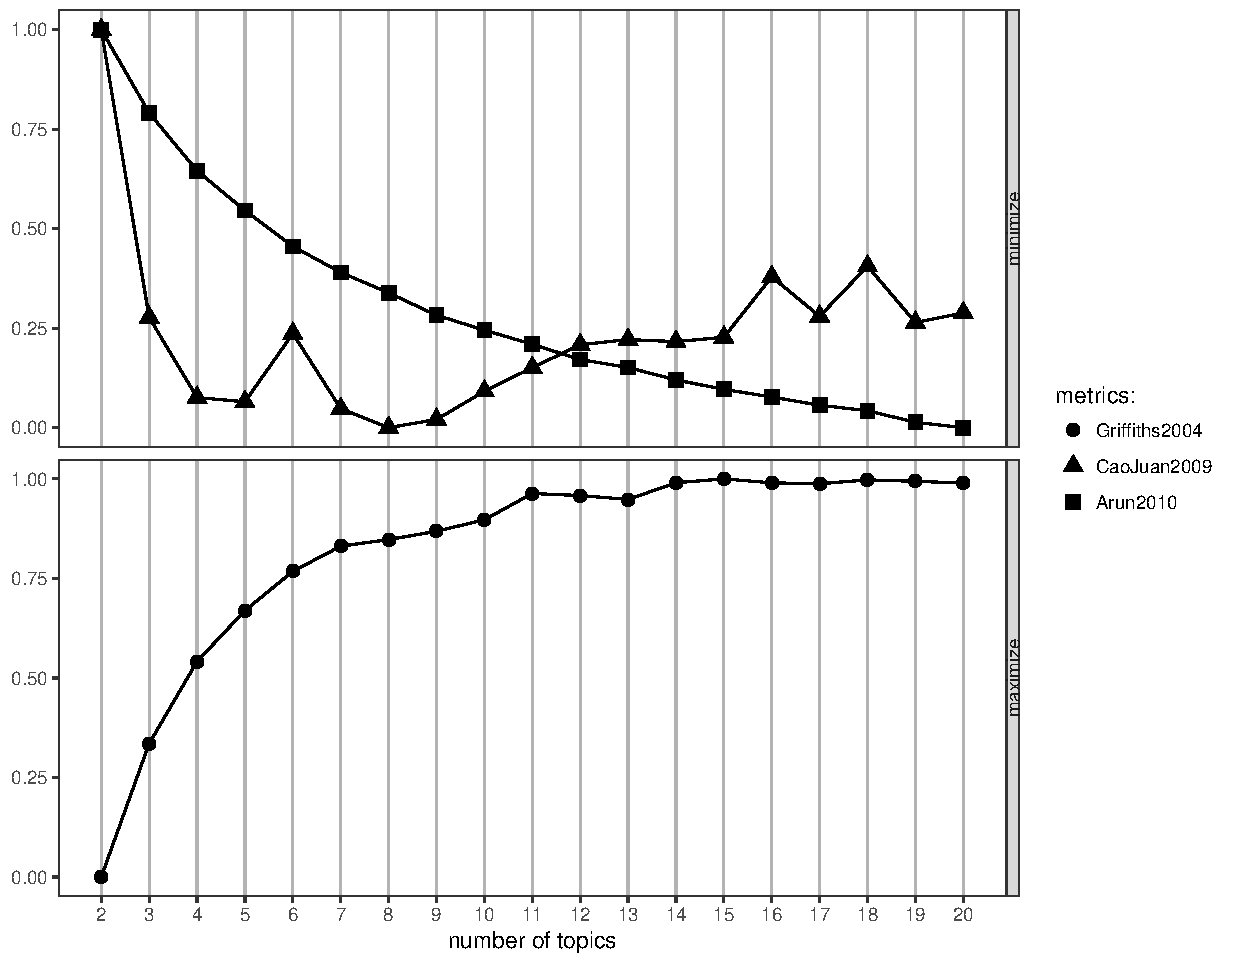
\includegraphics[width=0.6\linewidth]{_bookdown_files/figures/Griffithsetc} 

}

\caption{Relationship between the measures of the quality of the topic modelling output and the number of topics.}\label{fig:topicnumsm}
\end{figure}

We computed these for measures fitting a LDA model for every K between 2
and 20. We choose the higher value because we wanted to obtain a
reasonable number of topics representing the concepts (or we may say,
principles) behind sustainable manufacturing. The results of the
analysis are shown in figure \ref{fig:topicnumsm}. From this figure is
evident how the measure we want to minimize intersect each other at a
value between 11 and 12 topics. We thus decided to visualize the results
of the LDA models for a number of topics k between 7 and 15: the expert
panel interviewed then allowed to decide that the best results was at 12
topics.

\subsection{Results}\label{results-4}

We then extract the one-topic-per-term-per-row probabilities, beta. Beta
measures what is the probability for each topic to produce a term.
Figure \ref{fig:topicpicture} shows the top 5 terms for each topic. Here
each topic has a different vertical position and a different color. Each
topic is represented by a set of keywords and each keyword has a
different position on the y axes. For each intersection topic/keyword,
the dimension of a circle represent beta (what is the probability that
topic to produce that term). It is possible for some keywords to belong
to multiple topics: for example, optimization belongs to topic 1 and 9.
It is easy to spot these keywords because typically (belonging to two
different topics) are far from the group of keywords of the topics they
belong.

\begin{figure}

{\centering 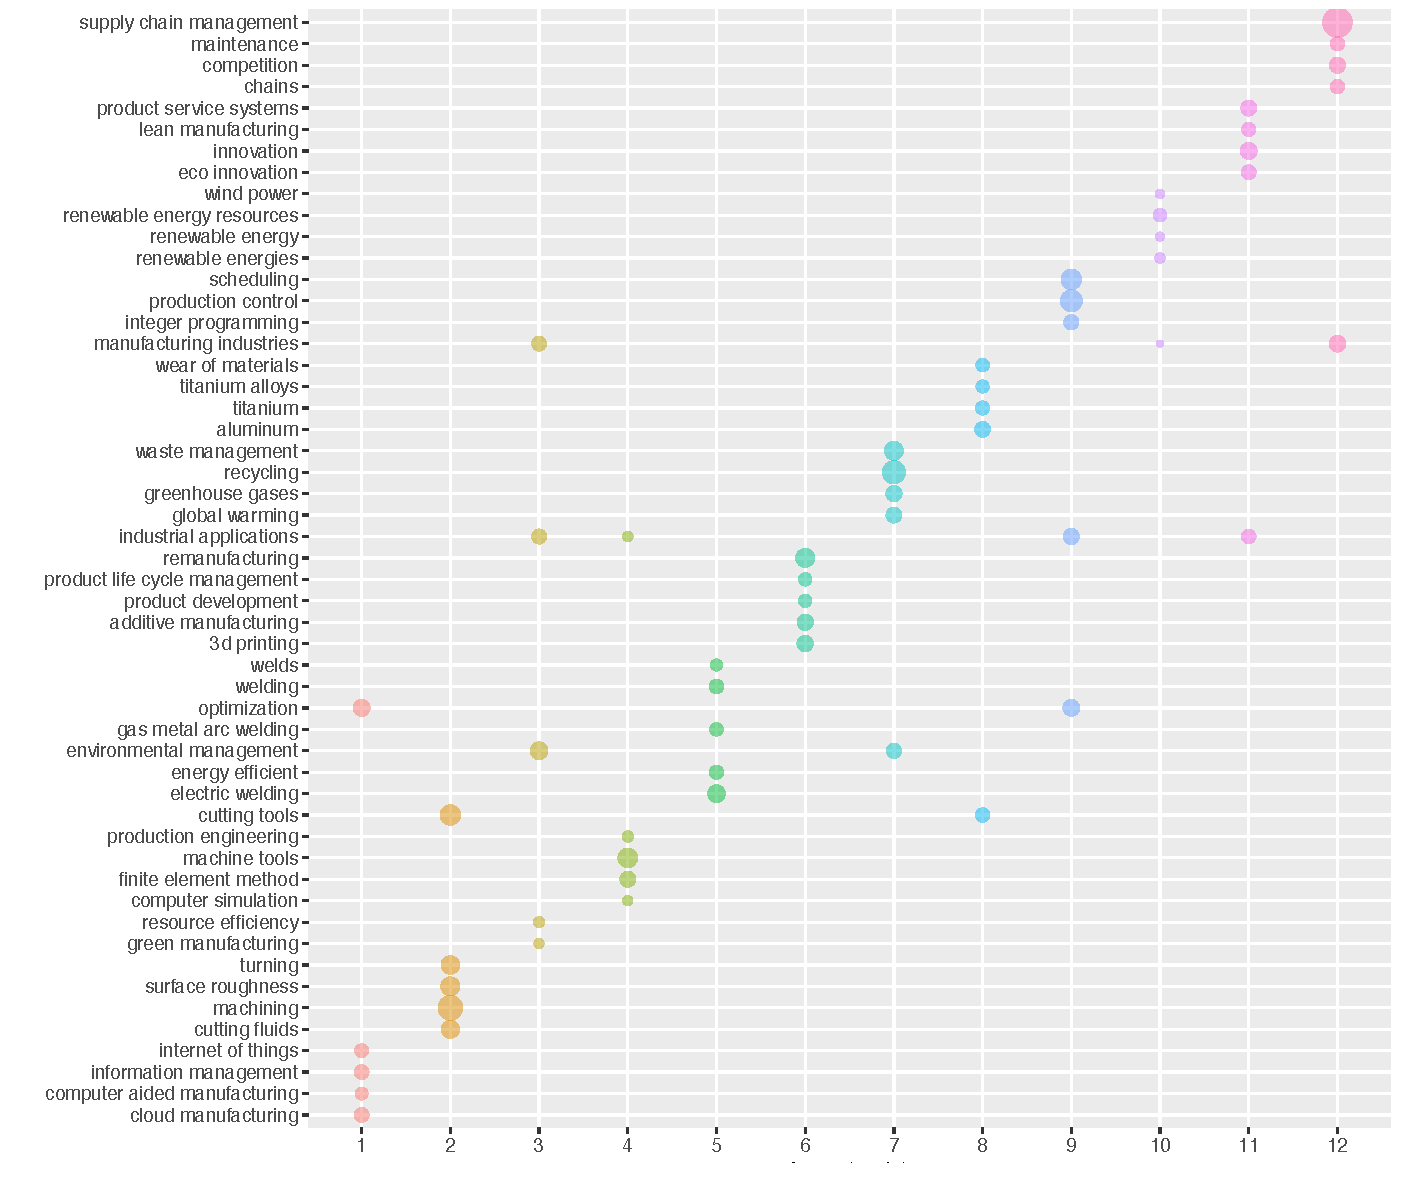
\includegraphics[width=1\linewidth]{_bookdown_files/figures/geom_point_topic} 

}

\caption{Content of the 12 topics. Each topic has a different vertical position and a different color. Each topic is represented by a set of keywords and each keyword has a different position on the y axes. For each intersection topic/keyword, the dimension of a circle represent beta (what is the probability that topic to produce that term).}\label{fig:topicpicture}
\end{figure}

\subsubsection*{Manual Labelling of the
topics}\label{manual-labelling-of-the-topics}
\addcontentsline{toc}{subsubsection}{Manual Labelling of the topics}

To have a clearer representation of the topics, these were manually
labelled by 6 independent experts in the field of manufacturing and
sustainability. Then a seventh experts took in input the results of the
manual naming and synthesized the label. The final results are the names
of the 12 topics. These names are:

\begin{enumerate}
\def\labelenumi{\arabic{enumi}.}
\tightlist
\item
  Smartness for Sustainability
\item
  Sustainable Machining
\item
  Manufacturing Environmental Efficiency
\item
  Modelling Manufacturing Sustainability
\item
  Welding Sustainability
\item
  AM Sustainability
\item
  Life-cycle Product Management
\item
  Advanced Material Sustainability
\item
  Production Management for Sustainability
\item
  Sustainable Energies
\item
  Innovation for Sustainability
\item
  Sustainable Logistic
\end{enumerate}

This final picture provides a clear representation of how topics
recognized are mostly homogeneous, provided there are few outlier
keywords per each topic, as in figure \ref{fig:topicpicture}. This ``new
perspective'' of sustainable manufacturing represents a way of defining
its contents by the grace of the tools or domain of interest involved.
For instance, topic n.1 (smart sustainability) refers to the use of the
new group of tools and approaches belonging to the Industry 4.0 stream,
thus defining specific contents and criteria useful to pursue the
sustainability in manufacturing.

\section{Blockchain}\label{blockchainanalysis}

In section \ref{advdrwresults} has been proposed a new usage of
sentiment analysis to extract advantages (considered synonym of the
words benefit, gain or profit) and disadvantages (drawback, failure) of
technologies from patents with the aim of helping researchers and
designers to effectively develop new products, analyzing positive and
negative properties of an innovation. The main contributions of the
present analysis is to list the problems of a technological field using
this sentiment tool. We want to understand which are the problems that
research is trying to solve for a technology and if is there any focus
from researchers on the solution of certain technical problem.
Furthermore using text mining techniques it is possible to correlate
these problems between them and understand if is there any correlation
between problems of technologies and if this map help researchers and
companies to understand the research agenda.

This section thus proposes an innovative methodology for the
(semi-automatic) extraction of technical knowledge from academic
articles, using text mining techniques. Among many information related
to technical knowledge, the methodology focus on the collection and the
analysis of the problems of a technology. The meaning of problems of a
technology is related to the concept of disadvantages of a technology
but with a broader sense. In fact, using papers as a source makes it
possible to collect not only technical disadvantages (typically
described in patents) but also, organizational, business or even social
problems, since these are faced by different intellectual fields in the
scientific literature. We also propose a case study on the application
of the method to the field of \emph{block-chain}. We chose this
technology because:

\begin{itemize}
\tightlist
\item
  It is highly innovative
\item
  It is having an impact in many different field
\item
  The problems of this technology are both technical and managerial
\end{itemize}

\subsubsection*{How Blockchain Technology
Works}\label{how-blockchain-technology-works}
\addcontentsline{toc}{subsubsection}{How Blockchain Technology Works}

The blockchain can be exemplified as a process in which a set of
subjects shares computer resources (memory, CPU, band) to make available
all private users in which each participant has a copy of the data.

The use of cryptographic validation techniques generates the mutual
trust of the participants in the data stored by the blockchain, which
makes it comparable to the registries managed in a centralized manner by
recognized and regulated authorities (banks, insurance companies, etc.)
\citep{pilkington201611}.

A blockchain is an open and distributed register that can store
transactions between parties in a safe, verifiable and permanent way.
Once written, the data in a block can not be retroactively altered
without the modification of all the subsequent blocks, and this, due to
the nature of the protocol and the validation scheme, would require the
consensus of the majority of the network. \citep{iansiti2017truth}

The blockchain is a continuously growing list of records, called blocks,
which are linked to each other and made safe by the use of cryptography.
Each block in the chain contains a hash pointer (that is a link to the
previous block), a timestamp and the transaction data.

The distributed nature and the cooperative model makes the validation
process robust and secure, but it has considerable time and costs, due
in large part to the \emph{price of the electricity} needed to validate
the blocks \citep{underwood2016blockchain}. Authentication takes place
through mass collaboration and is fueled by collective interests. The
result of all this is a robust workflow where participants' data
security expertise is not required. The use of this technology also
makes it possible to overcome the problem of the infinite
reproducibility of a digital asset and of the double expense without
using a central server or an authority. \citep{karame2012double}

There exist an overtrust about blokchain technology for businesses, and
there exist a growing interest about the drawbacks of this technology
\citep{eyal2018majority, lin2017survey, yli2016current}. Has been
pointed out that a 51 percent attack 26 would be enough to access or
control a private blockchain because, in most cases, the organization
that controls it already controls one hundred percent of the block
creation. In fact, if someone could attack or damage the blocking tool
on a private company server, would be possible to get complete
management of the network and the ability to access and modify the data
\citep{hampton2016understanding}. This is because the centralization due
to the privatization of the blockchain leads to a single point of
failure, or a central break point, which in a public blockchain could
not happen as distributed, so there would be no central point to attack.
This could have profound implications in financial crises or debt crises
like the 2007-08 financial crisis.

\subsection{Methodology}\label{methodology-4}

Considering our objectives, the approach we adopted for paper analysis
is radically new with respect to the one traditionally established in
the literature (bibliometric analysis and keyword approaches). These
approaches do not allow a deeper understanding of the technical content
described in the text. For this reason, we relied on text mining
techniques supported by our technical knowledge base. For the sentiment
computation in fact, we used a technical sentiment lexicon developed by
the authors that extracts advantages and disadvantages of inventions
from patents (\ref{advdrwresults}) and a novel dictionary lockup
approach that incorporates weighting for valence shifters. Following a
bottom up-approach, we redesigned and updated these lexicons for an
optimal application to paper documents.

\begin{figure}

{\centering 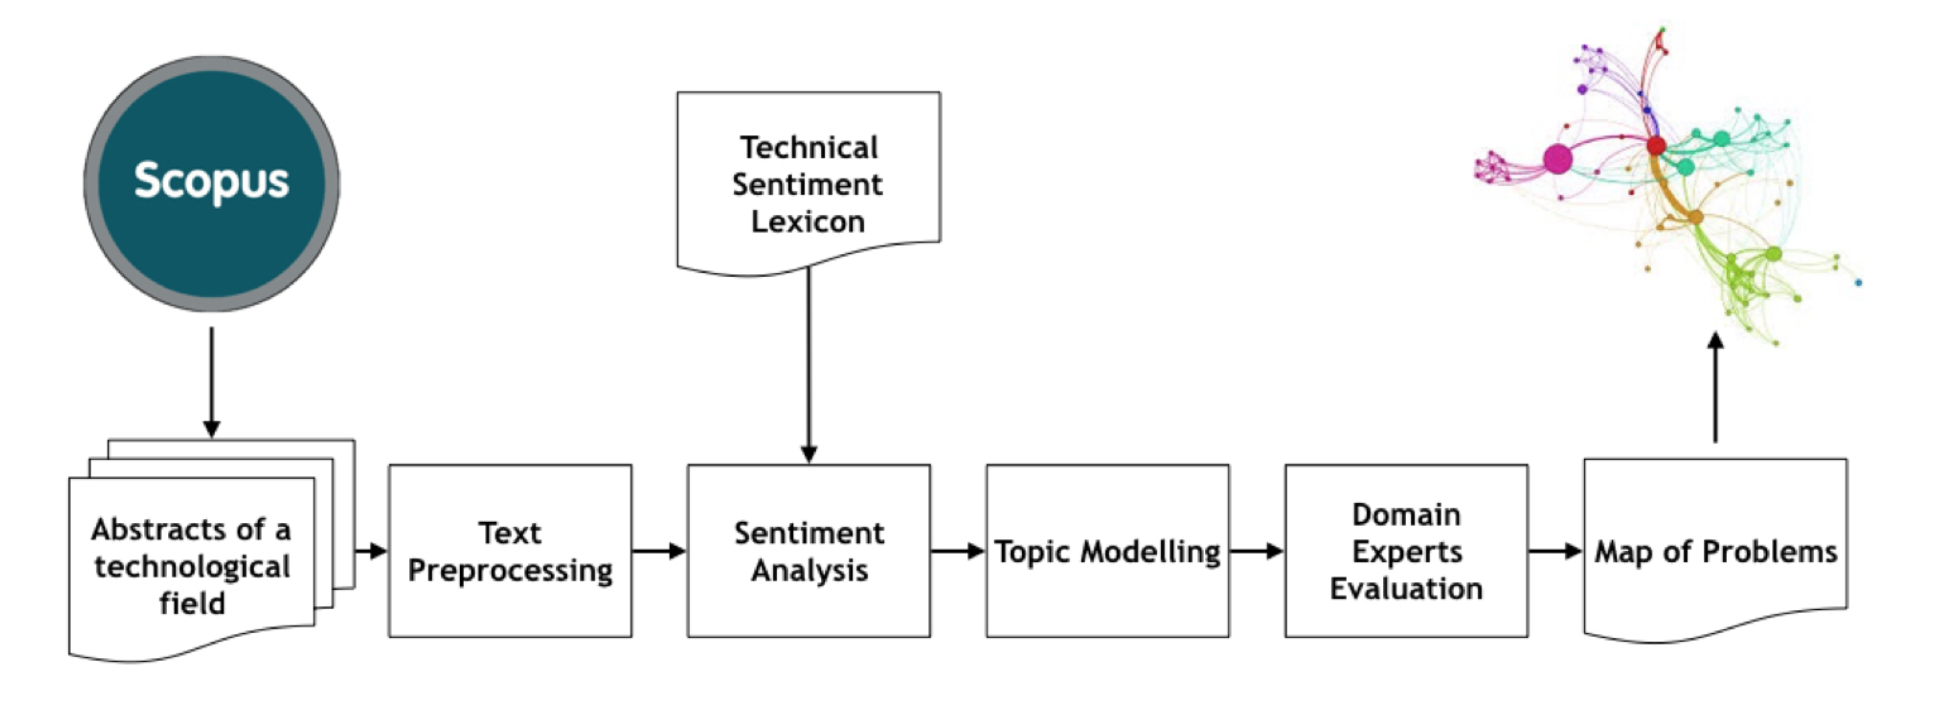
\includegraphics[width=0.8\linewidth]{_bookdown_files/figures/bcworkflow} 

}

\caption{Proposed workflow for the problem extraction from papers. }\label{fig:bcworkflow}
\end{figure}

The workflow of the proposed methodology is shown in figure
\ref{fig:bcworkflow}. The process starts with the collection of
abstracts belonging to the same technological field. The abstracts are
downloaded using the Scopus API, extracting all the documents that
contains keywords of the selected technology in the title, abstract or
keywords fields. The texts are then pre-processed using state of the art
natural language processing tools (sentence splitter, tokenizer,
lemmatization). Then, for each sentence we computed a negative sentiment
polarity and took into consideration only the sentences having a
negative polarity score below a threshold level. We applied topic
modelling algorithm on the negative sentences with the aim of
clustering. The output of topic modelling is evaluated by technology
domain experts with the aim of labeling the identified clusters.

The application scenarios of our methodology have a wide range of users:

\begin{enumerate}
\def\labelenumi{\arabic{enumi}.}
\tightlist
\item
  Companies that want to rapidly map a certain technological field
\item
  Policy maker that want to invest to solve problems of a technology to
  boost its innovation
\item
  Journals, to understand the hot-topic of a specific field
\item
  Research networks, to exploit possible collaborations and synergies
  between scholars.
\end{enumerate}

\subsubsection*{Document collection and
selection}\label{document-collection-and-selection}
\addcontentsline{toc}{subsubsection}{Document collection and selection}

The documents were extracted from Scopus searching for the query:

\begin{equation*} 
  TITLE-ABS-KEY("blockchain" OR "block chain" OR "block-chain")
\end{equation*}

At the date of 29/05/2018 the query results in 1,628 documents.

The term blockchain and its morphological variations is used in other
fields different from computer science and economics, in particular in
chemistry. For this reason we filtered from the data set all the papers
belonging to one of the sequent All Science Journal Classification
(ASJC) classes: chemistry, physics and astronomy, chemical engineering,
biochemistry, genetics and molecular biology, pharmacology, toxicology
and pharmaceutics, immunology and microbiology. The result of this lead
us to a set of 1,364 papers.

To have a dataset with an higher precision, we also filtered using rules
based on the content of the abstracts, since many conferences do not
have an ASJC class in Scopus. This characteristic of the Scopus database
could lead to bias in the results, especially for innovative
technologies like block-chain for which the scientific discussion is
stronger in conferences then in more structured journals. For this
reason we analyzed the abstracts of the 264 articles belonging to one of
the ASJC classes listed above (chemistry related) extracting the most
frequent words and filtering for a blacklist of generic words contained
in scientific articles. This results in a dictionary of words that has
been used to search and filter al the papers containing in the abstract
one or more of the words in the dictionary. The final number of selected
papers is 1,276.

\subsubsection*{Sentence Splitting}\label{sentence-splitting}
\addcontentsline{toc}{subsubsection}{Sentence Splitting}

A sentence splitter (for further details see section
\ref{sotatoolstransformsentencesplit}) is then applied to the abstract
to divide the texts in sentences. From this step we had an output of
8,406 sentences.

\begin{figure}

{\centering 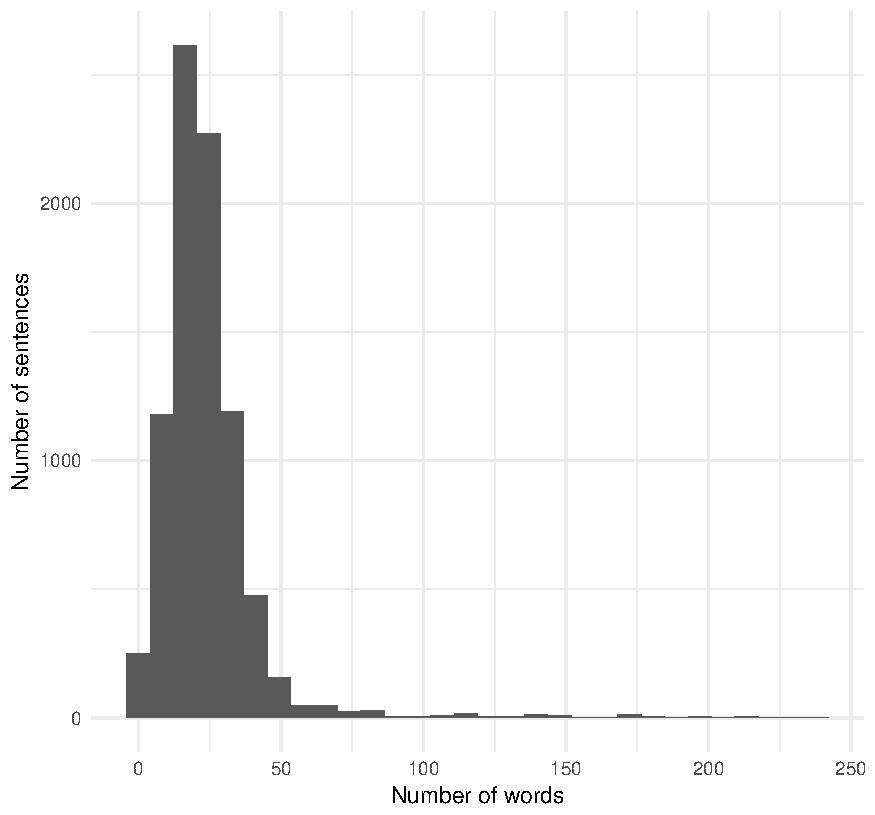
\includegraphics[width=0.8\linewidth]{_bookdown_files/figures/length_histogram_bl} 

}

\caption{Histogram of the lengths of the sentences.}\label{fig:histbllength}
\end{figure}

The next step involved the measure of the sentences length. Some of the
sentences in fact could be too long due to several fact for example the
style of the author or an error in the sentences splitting phase). Since
it is not a goal of the present work to analyze the style of the authors
or to design a better sentence splitter, we decided to filter the
sentences that are too long. The decision on the threshold level of
number of word has been taken analyzing the distribution shown in figure
\ref{fig:histbllength}. The 97\% of the population of sentences contain
a number of words that is lower than 53. Thus all the sentences contain
more than 53 words has been filtered. From this step we had an output of
8143 sentences.

\subsubsection*{Polarity Computation}\label{polarity-computation}
\addcontentsline{toc}{subsubsection}{Polarity Computation}

At this point has been possible to apply a sentiment polarity
measurement on the sentences \citep{sentimentr2018}. As output we had a
polarity score between -1 (strongly negative) and 1 (strongly positive)
for each sentence. Since we are interested in extracting the problems of
the state-of-the-art blockchain systems, we visualize the distribution
of the polarity scores of the sentences labeled as negative (having a
polarity score lower then 0). The histogram of this distribution is
shown in figure TOT. In this histogram are represented 1,108 different
sentences. As we can see we have a distribution center in -0.2, with a
tail that goes down to -0.8. This is an evidence that the system give a
reasonable measures since it would be unreasonable to have more probable
extreme values. Furthermore, the number of sentences having a polarity
equal to 0 is 4,435 that is about the 50\% of the sentences and the
number of sentences having a positive polarity is 2,700 : it is
reasonable that the higher number of sentences falls in these classes
since the scientific jargon has to be neutral. The positive bias has
been seen also for patent documents (see section \ref{advdrwresults})).

\begin{figure}

{\centering 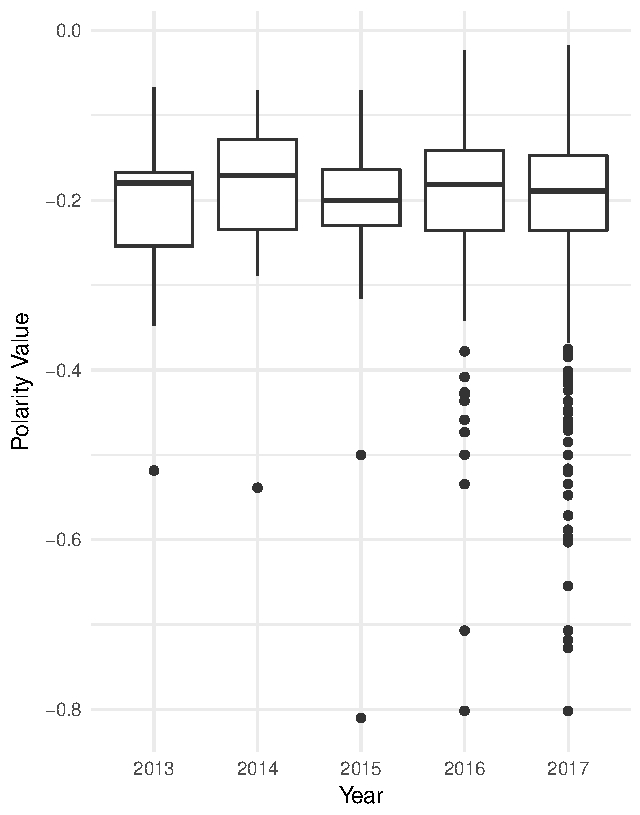
\includegraphics[width=0.5\linewidth]{_bookdown_files/figures/polarity_histogram_time_bl} 

}

\caption{Box plots of the distributions  by years of the polarities of the sentences having a negative polarity score.}\label{fig:sentintimebl}
\end{figure}

One interesting evidence we found is that the number of outliers (having
a polarity values lower than the 95\% of the population) is growing over
the year as shown in figure \ref{fig:sentintimebl}. Even if the mean
remains near to -0.2, int he last five years the number of strongly
negative sentences has increased. This shows how there has been a trend
in the focus on the problems of blockchain.

\subsubsection*{Tokenization and Token
Filtering}\label{tokenization-and-token-filtering}
\addcontentsline{toc}{subsubsection}{Tokenization and Token Filtering}

In the next phase we apply a state of the art natural language
processing pipeline (see section \ref{sotatools} for more details) to
the 1,108 negative sentences.

The tokenization process results in 220,094 tokens. To extract the
meaningful words (words that adds information about the problem that the
sentence is describing) we applied a series of filtering steps. As
meaningful unit to analyze (token) we decided to use the lemma of the
word. The 9,451 final token is a reasonable number considering the 1,108
sentences in input: we have a mean of 9 words per sentence. Considering
the mean of 25 words per sentence shown in figure
\ref{fig:histbllength}, we now have a summary of the sentences contains
only the meaningful words. This output is a clean input for the topic
modelling phase.

\subsubsection*{Topic modelling}\label{topic-modelling}
\addcontentsline{toc}{subsubsection}{Topic modelling}

Topic modeling is a method for unsupervised classification of documents
which finds groups of documents fitting a statistical model to the data.
In other words, these models captures word correlations in a collection
of documents with a set of topics. Latent Dirichlet allocation (LDA) is
a particularly popular method for fitting a topic model. It treats each
document as a mixture of topics, and each topic as a mixture of words.
This allows documents to ``overlap'' each other in terms of content,
rather than being separated into discrete groups, in a way that mirrors
typical use of natural language (for further details see section
\ref{sotatoolsmodeltopicmodel}). If the topic modelling process is good,
we have as output a structure where every topic is an understandable,
meaningful and compact semantic cluster that in our case clearly
represent a state-of-the-art problem of block chain technology.

\subsubsection*{Document Term Matrix}\label{document-term-matrix}
\addcontentsline{toc}{subsubsection}{Document Term Matrix}

The first step is to take in input the 9,451 tokens and count how many
times each one occurs in the 1,108 sentences. In this way we obtain a
document-term matrix (DTM) where the documents are the sentences and the
terms are our tokens (the lemmas). In our case the DTM has 1077 rows
representing the sentences (31 sentences did not contain any relevant
tokens) and 1147 tokens.

\subsubsection*{Definition of the Optimal Number of Topics: a
Human-Machine Hybrid
Approach}\label{definition-of-the-optimal-number-of-topics-a-human-machine-hybrid-approach}
\addcontentsline{toc}{subsubsection}{Definition of the Optimal Number of
Topics: a Human-Machine Hybrid Approach}

To fit a LDA model we have to give as a parameter the number of topic k
that we think that best represent the corpus in analysis. In literature
there exists many measurement to compute an optimal value of k. However
it is worth to keep in mind that these measures are not always
correlated with expert judgement about topics interpretability and
coherence. For this reason in the present section we use an hybrid
approach in which we find an optimal neighborhood of value using state
of the art k tuning methods and then we compute a graphical output for
the 5 best k values to be evaluated by 4 different experts.

Several approaches tried to take the problem of automatically finding
the right number of topics contained in a set of documents. Every
approach follow the idea of computing distances (or similarities)
between pair of topics varying the number of topics. We used four
different methods to evaluate the output of a topic model for different
value of k. These methods are:

\begin{itemize}
\tightlist
\item
  \emph{Caojuan2009} \citep{cao2009density}: Minimize the average cosine
  distance between every pair of topics. The best topic number K has a
  minimal final distance between topics in Latent Dirichlet Allocation
\item
  \emph{Arun2010} \citep{arun2010finding}: Minimize the symmetric
  KL-Divergence of the salient distribution that are derived from the
  matrices of factors. These matrices are the re-projections of the
  documents on the topics and of the topics on the vocabulary (the
  selected tokens). The divergence values are higher for non-optimal K
  values.
\item
  \emph{Griffiths2004} \citep{griffiths2004finding}: Maximize the likely
  of the data given the model built considering K topics. This is a
  problem of model selection using Bayesian statistics.
\item
  \emph{Deveaud2014} \citep{deveaud2014accurate}: Maximize the
  information divergence between all pairs of topics. The optimal value
  k is the value for which LDA modeled the most scattered topics.
\end{itemize}

\begin{figure}

{\centering 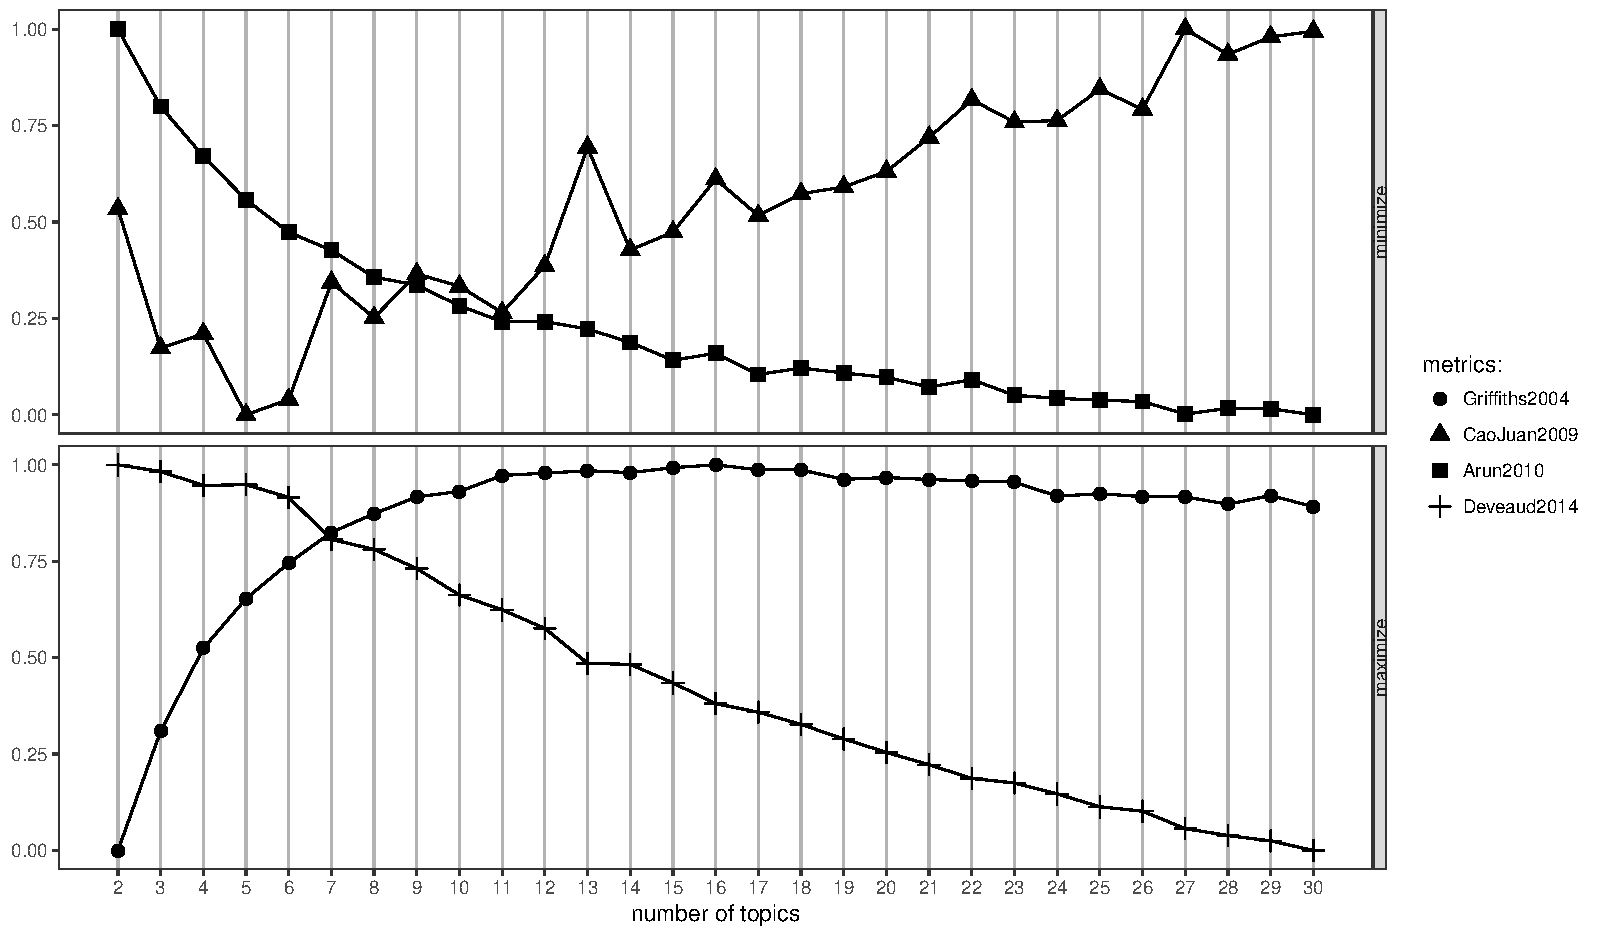
\includegraphics[width=0.6\linewidth]{_bookdown_files/figures/FindTopicsNumber_plot_bl} 

}

\caption{Measures of quality of the topic modelling results for growing number of topics. The figure is divided in metrics to minimize (top figure) and to maximized (bottom figure).}\label{fig:topicnumsmbl}
\end{figure}

We computed these for measures fitting a LDA model for every K between 2
and 30. We choose the higher value because we wanted to obtain a
reasonable number of topics representing the problems of blockchain.
After a brain storming with experts it emerges that there can not exists
more than 15 classes of problems. We decide to take the double of this
number to take in to consideration the biases of human experts. The
results of the analysis are shown in figure \ref{fig:topicnumsmbl}. From
this figure is evident how the measure we want to minimize interest each
other at a value of 7 topics; the values we want to minimize are a
little more unstable (especially \citep{arun2010finding}) and intersect
both at level of 9 and 11. We thus decided to visualize and make choose
the results of the LDA models for a number of topics k between 7 an 10.

To help experts in their decision process, an interactive map of the
problem has been generated for 7, 8, 9, 10 and 11 topics. The map was
created using Shiny \citep{shiny2017}. The interactive map of problems
(a screen shot of the app is shown in figure
\ref{fig:topicmodelschinybc}) helped experts to understand the
relationships between the problems. Here a multidimensional scaling
algorithm compute the inter-topic distance that permits to visualize the
distribution of topics in two dimensions. Clicking on a topic the
experts can see its content, and for each word can see both at the
estimated term frequency within the selected topic and at the overall
term frequency.

\begin{figure}

{\centering 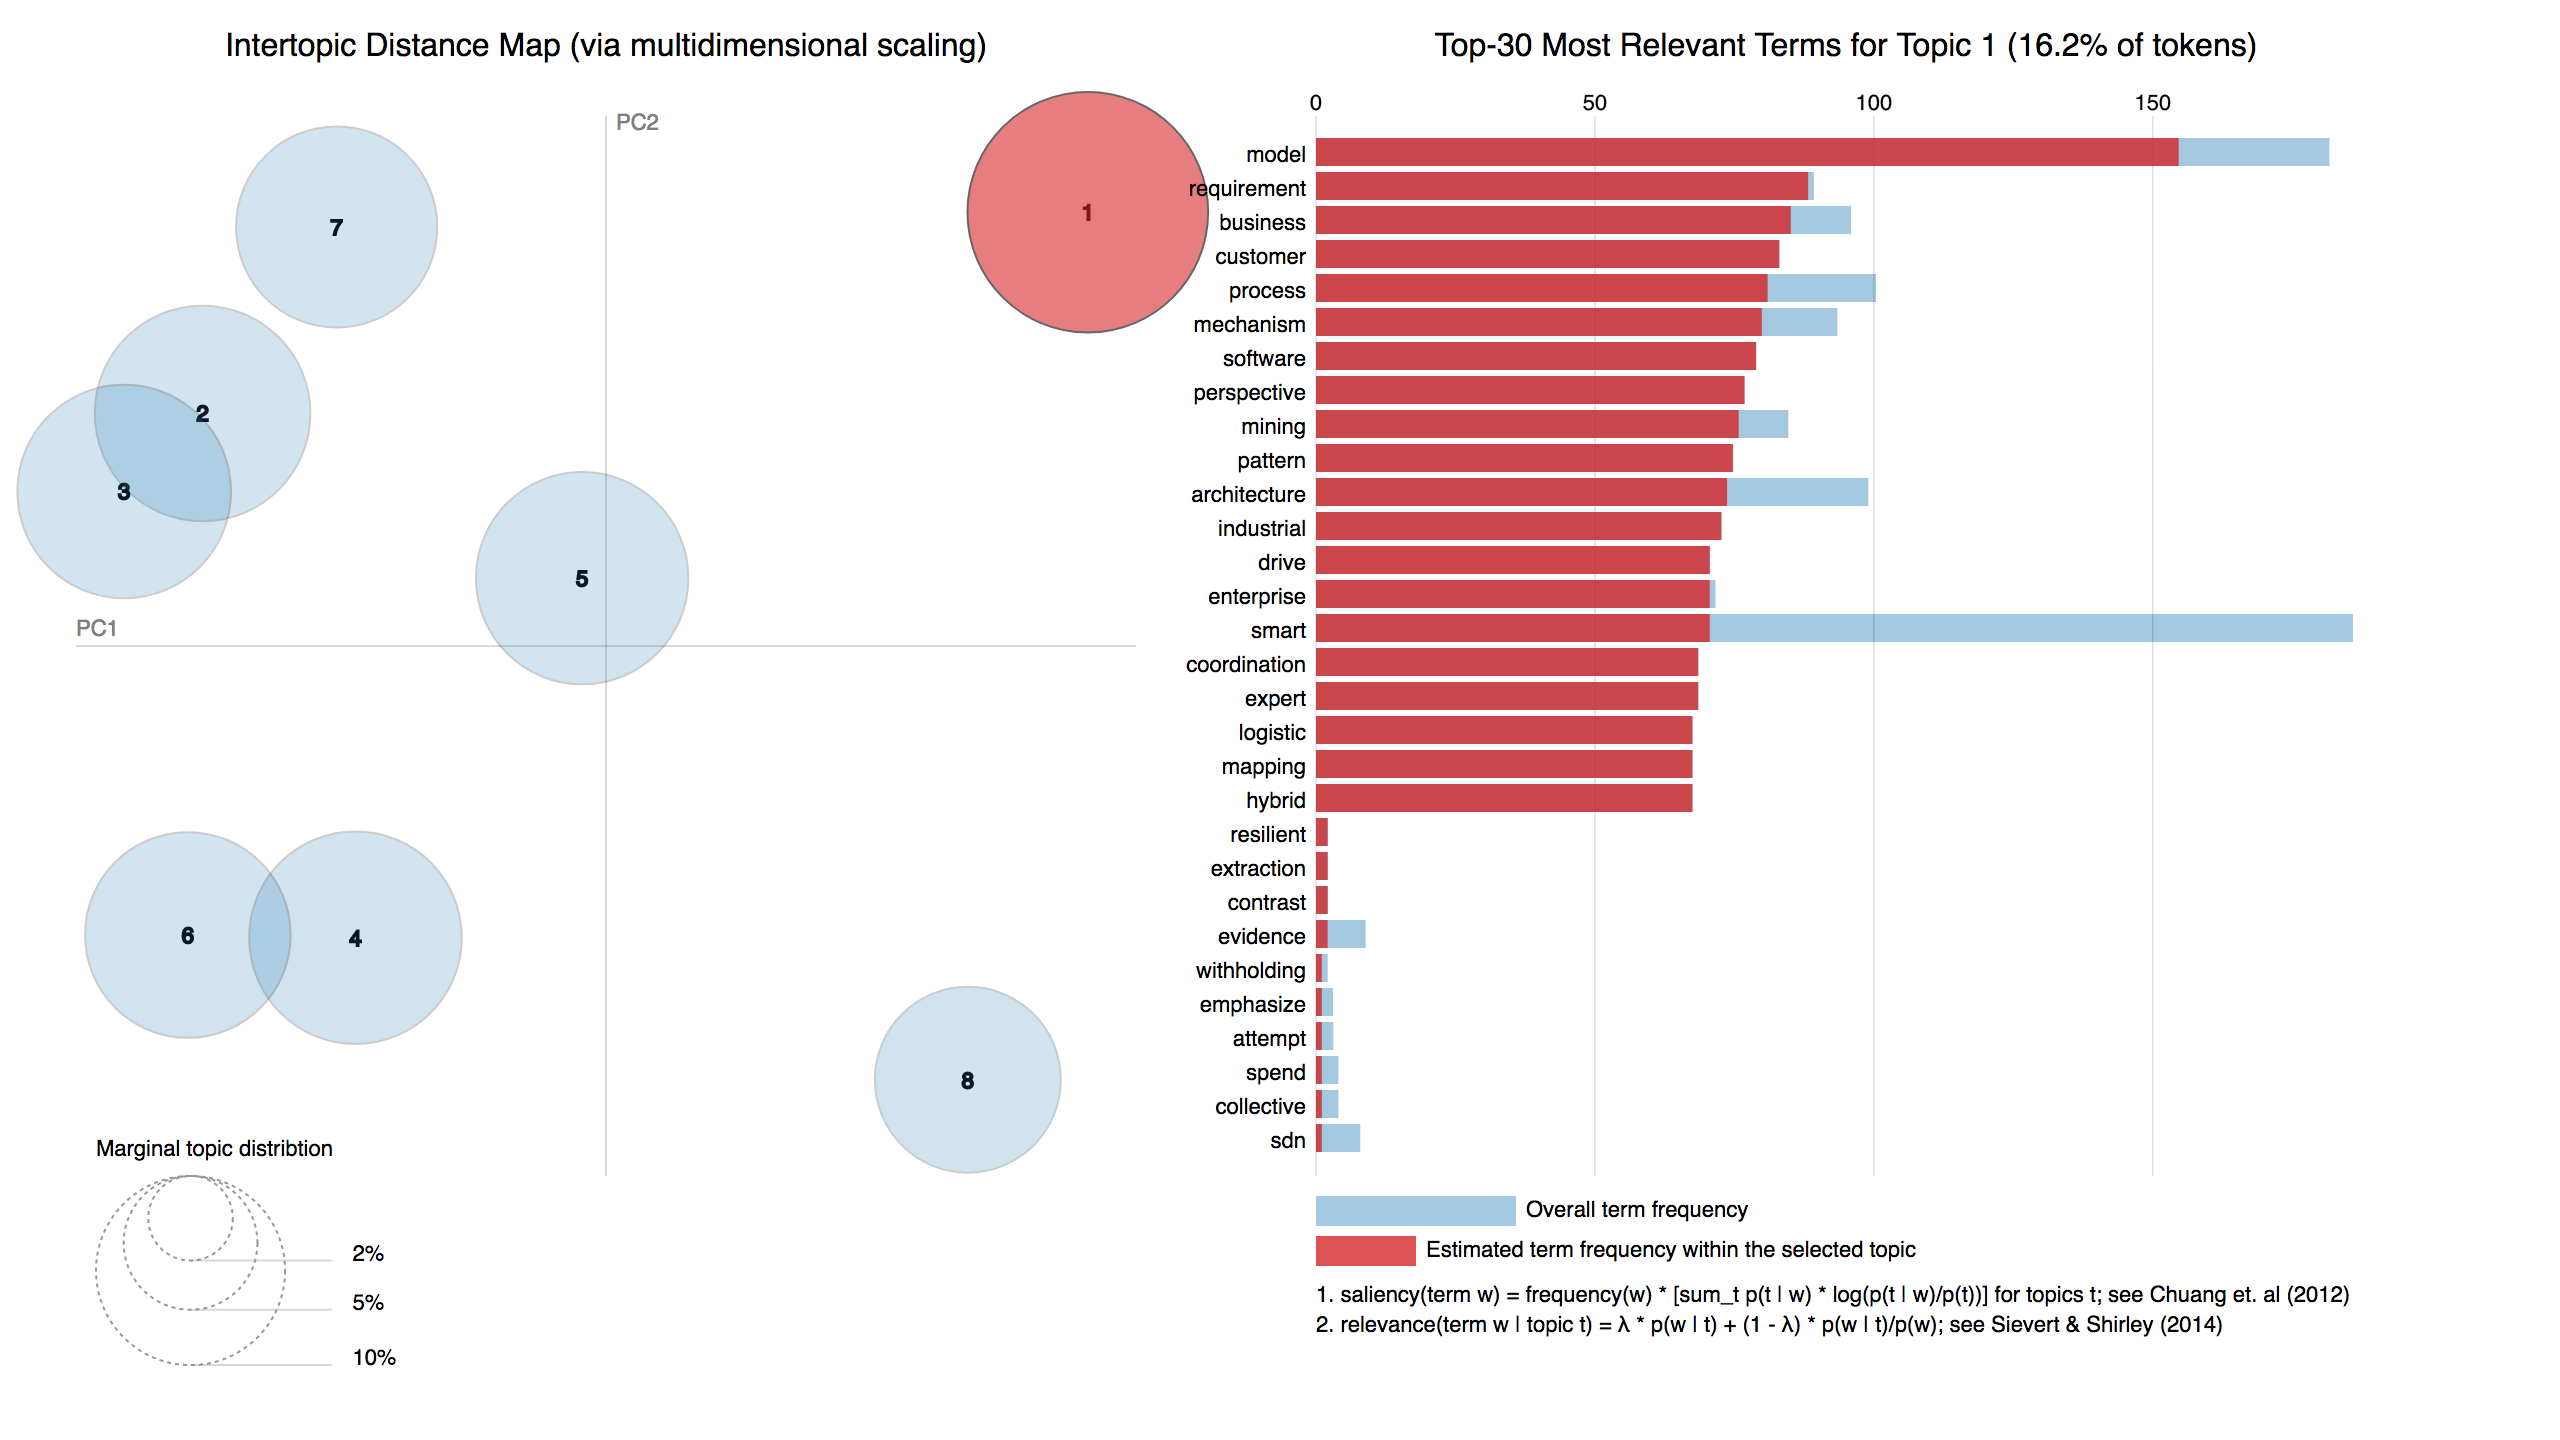
\includegraphics[width=0.8\linewidth]{_bookdown_files/figures/bc_topicmodel_shiny} 

}

\caption{Screenshot of the shiny app used by experts to choose the optimal number of topcis. }\label{fig:topicmodelschinybc}
\end{figure}

The experts agreed for a total number of 8 topics as optimal.

\subsection{Results}\label{results-5}

The output topic modelling phase is show in figure
\ref{fig:topicmodelsoutputbc}. The results of the topic modelling are
visualized to make it possible for the expert to explore and label the
topic representing the problems of block chain technology. Each point is
a word, and word belonging to the same topic are grouped. The size of
the label is proportional to the probability ß that the word belong to
that topic.

\begin{figure}

{\centering 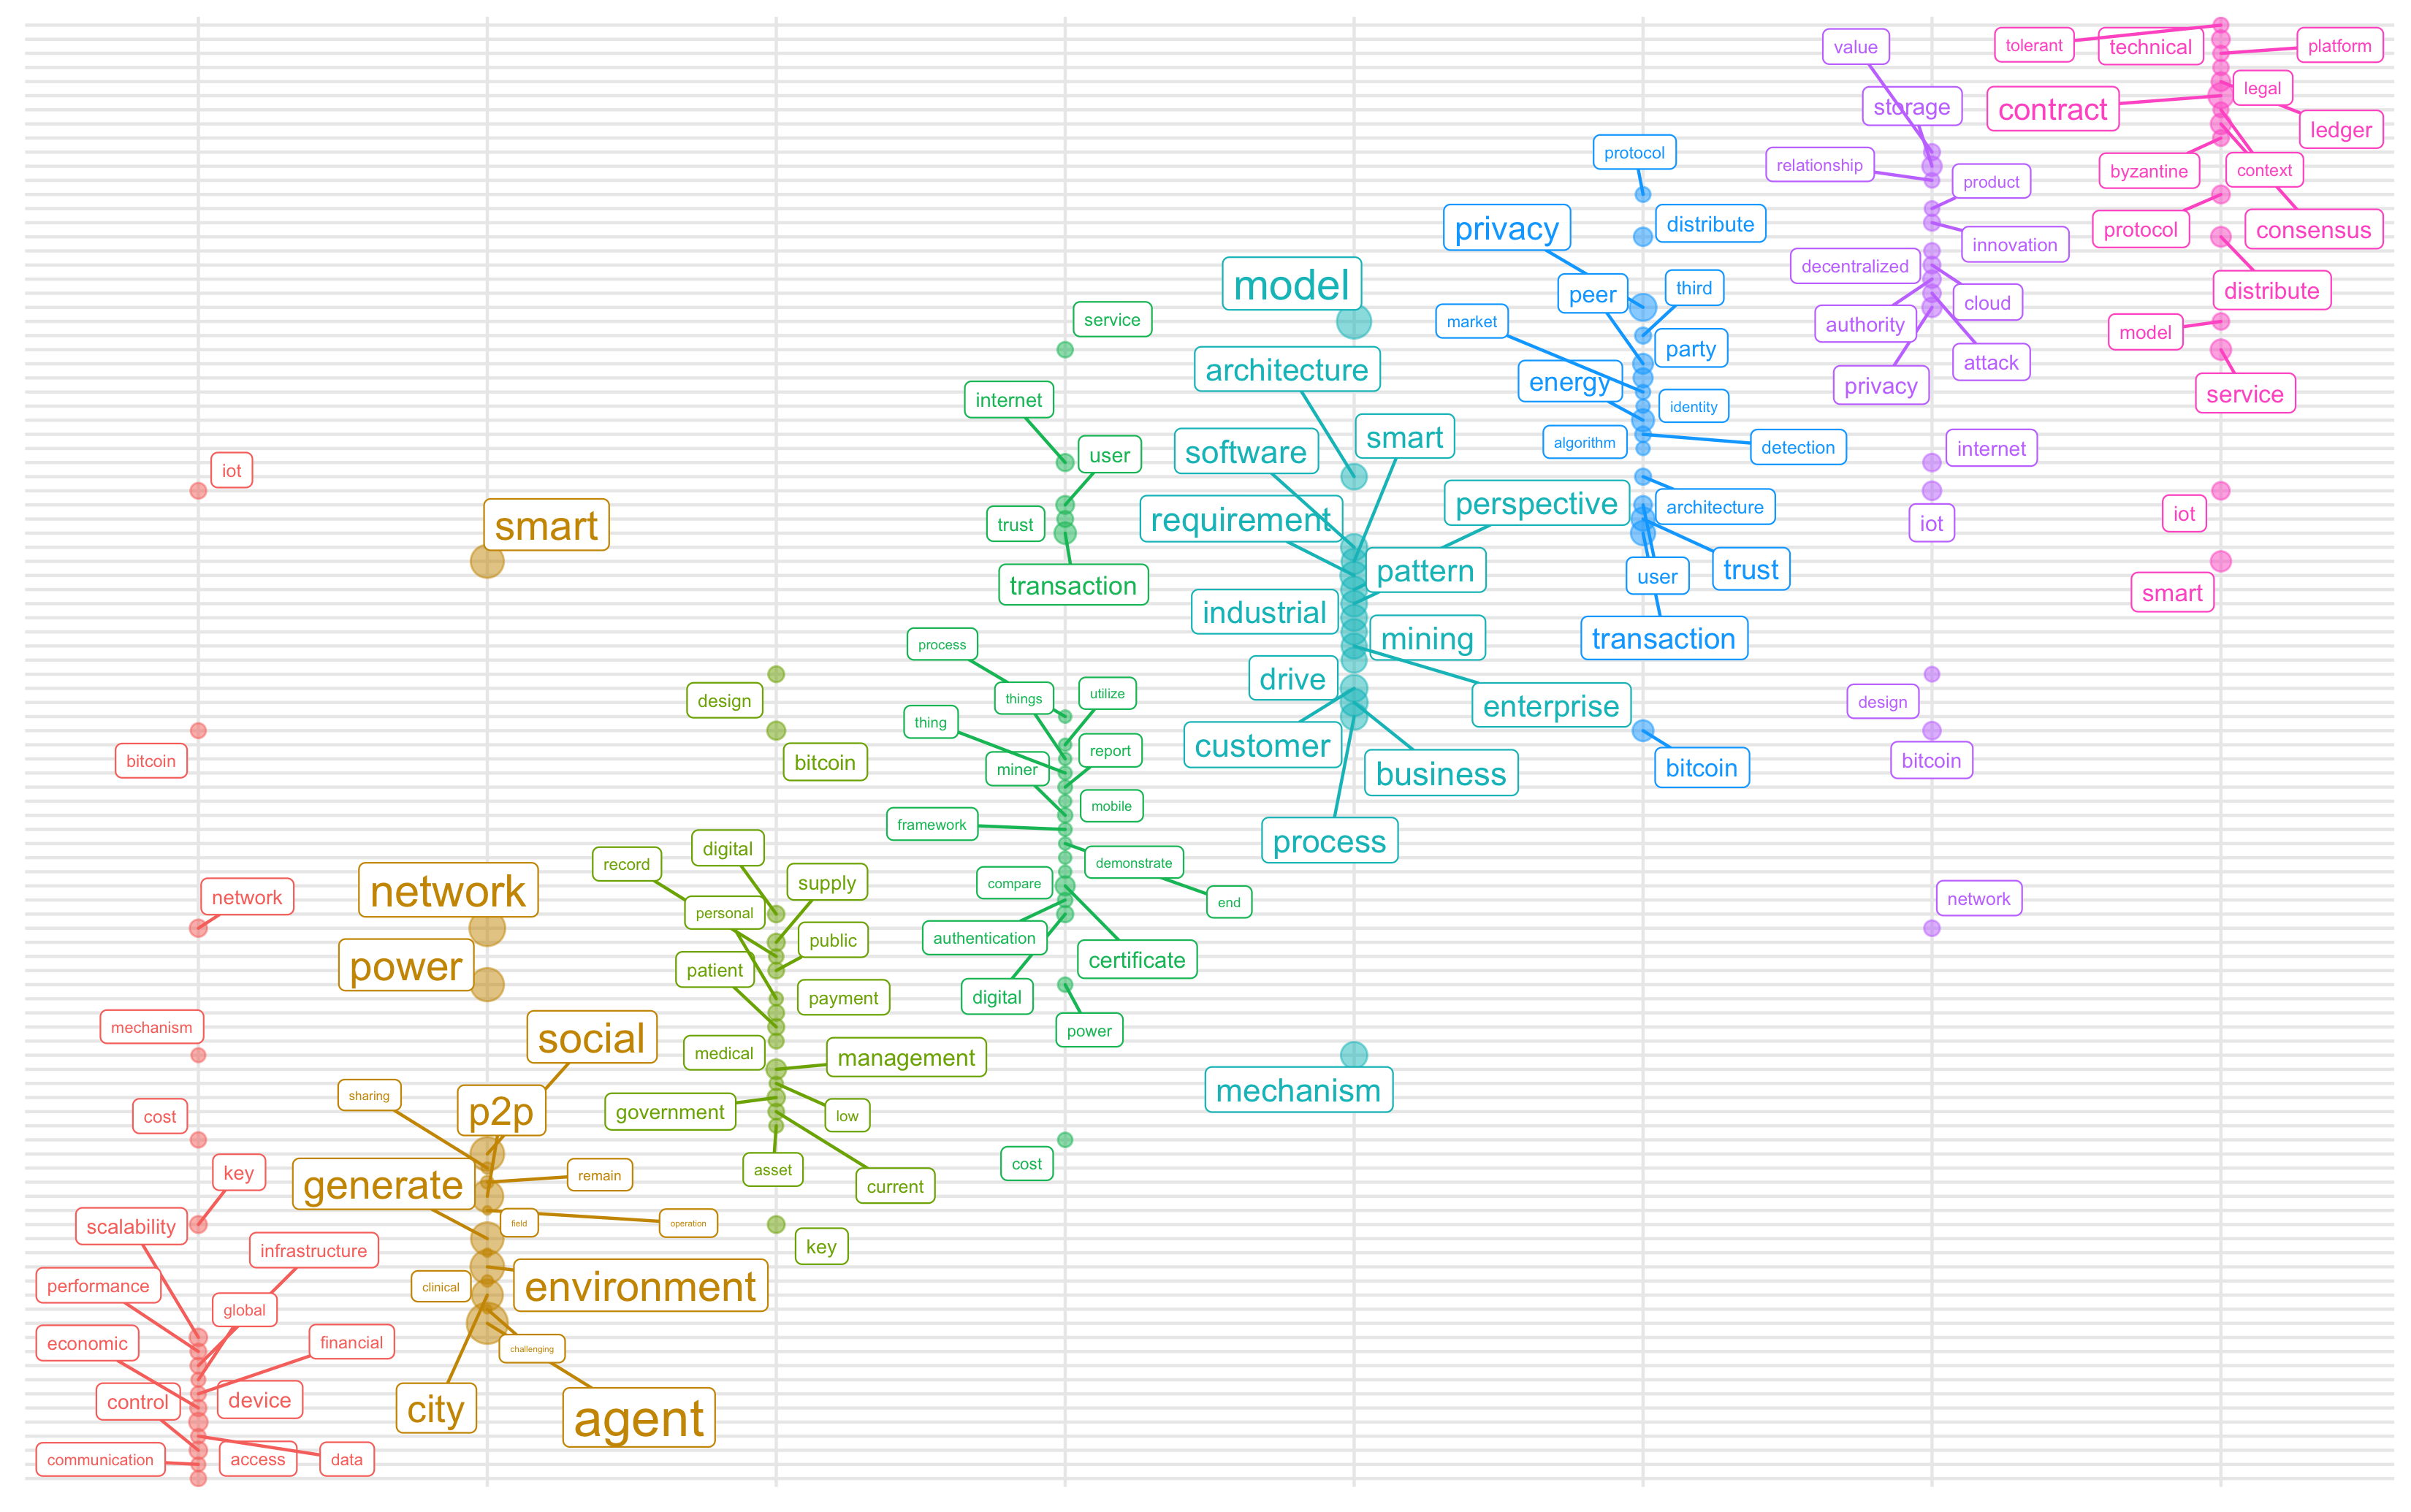
\includegraphics[width=0.8\linewidth]{_bookdown_files/figures/output_bl_topicmodels} 

}

\caption{Content of the 8 topics of problems of blockchain. Each topic has a different vertical position and a different color. Each topic is represented by a set of keywords and each keyword has a different position on the y axes. For each intersection topic/keyword, the dimension of a circle represent beta (what is the probability that topic to produce that term}\label{fig:topicmodelsoutputbc}
\end{figure}

\section{Precision Agriculture}\label{precisionagri}

The agriculture is facing rapidly changing economic, social and
environmental scenarios in 21st Century. Forecasts on worldwide
population estimate that it might increase at about 9 billion by 2050
and led the Food and Agriculture Organization of the United Nations
(FAO) to underline the growth of food needs of about 60\% if compared to
the annual average calculated between 2005 and 2007. The Committee on
Agriculture and Rural Development of the European Parliament confirms
these figures. In this regard, FAO focuses on how global agricultural
and food systems can support the subsistence needs of the worldwide
population according to different cultures and dietary habits of both
developed and emerging countries.

Compared to past agricultural policies, nowadays trends related to
technological evolution, socio-political changes, water shortages, as
well as the increase in energy needs and the emergence of new pests and
diseases that affect agricultural production acquire greater importance
in the discussion between policy makers and companies concerning the
future of agricultural activities.

In particular, technological innovation is necessary for the development
of companies which aim to strengthen their production processes and
organizational structures by exploiting automation and ICT within the
cultivation and commercialization processes. Thus, digital technologies
at the base of Precision Agriculture are the assets to leverage to deal
with two major challenges for modern agriculture. On one hand, the need
for an increase in production quantity by optimizing production factors.
On the other hand, complying with production standards by combining
appropriate quality levels and limited environmental impact. Precision
Agriculture is a modern approach for agricultural management that
exploits cutting-edge technologies to monitor and optimize agricultural
production processes.

The concept of Precision Agriculture was born in the United States in
the early nineties, where the House of Representatives
\citep{liaghat2010review} defines it as ``an integrated information- and
production-based farming system that is designed to increase long term,
site-specific and whole farm production efficiency, productivity and
profitability while minimizing unintended impacts on wildlife and the
environment''. Although it is a relatively well-known concept, Precision
Agriculture still presents a low rate of adoption as reported by both
academic surveys and professional reports \citep{pierpaoli2013drivers}.

Different definitions given by researchers, practitioners and policy
makers have gradually allowed to deepen the understanding of the
constituent elements of the concept as shown in the following table.
Table 1 presents a literature review carried out on the Scopus database
focusing on the analysis of the definitions of the concept of Precision
Agriculture, and shows how technology emerges as the enabling aspect of
Precision Agriculture. Anyway, authors focused also on other elements
that refers to Precision Agriculture.

Pierce and Nowak \citep{pierce1999aspects} highlight the centrality of
Technology and Benefits as the two key elements of Precision
Agriculture. Zhang et al. \citep{zhang2002precision} strengthen these
two distinctive elements, which compare in all subsequent analyses
\citep{stafford2000implementing, kirchmann2000challenging}, until the
introduction of the concept of Sustainability
\citep{bongiovanni2004precision}. Indeed, Bongiovanni emphasizes the
environmental topic by underlining the role of Precision Agriculture to
manage harvest production inputs in an environmentally friendly manner.
Finally, Gertsis et al. \citep{gertsis2018lisa}, define Precision
Agriculture as ``A modern farming management concept using digital
techniques to monitor and optimize agricultural production processes''.
They introduce the concepts of digital techniques and optimization of
production processes by highlighting some possible concrete applications
of Precision Agriculture. As emerged from the previous analysis, a
fundamental role for the implementation of Precision Agriculture is
played by digital technologies. In particular, object identification,
georeferencing, measurement of physical and chemical parameters,
satellite navigation, connectivity, data storage and analysis, process
automation and vehicle driving are the most adopted
\citep{schrijver2016precision}. Precision agriculture is then based on a
cyclical process of observation and acquisition of data, followed by an
interpretation and evaluation of the information acquired, and by the
implementation of a series of decisions that respond to them. Thanks to
these technologies, farmers can increase production, optimize resources
consumption (workforce included), costs and quantitative and qualitative
production possibilities, according to the specific characteristics of
the soil and cultivation. \citep{sawant2016organized} shows that the
implementation of digital technology in agriculture can increase total
profitability from \$ 55 to \$ 110 per acre (1 acre = 4046.87 m²).

However, whether the Precision Agriculture is still far from being
widely adopted \citep{pierpaoli2013drivers, tey2012factors}. Indeed, the
implementation difficulties related to the high initial investments and
the lack of suitable skills among the farmers identified still represent
significant obstacles. In fact, a study conducted by Pierpaoli et al.
\citep{pierpaoli2013drivers} identifies the so-called ``non-adopters''
farmers, (e.g.~those who do not have sufficient skills or financial
resources to manage the PA's instruments). For these reasons measuring
the concrete benefits of Precision Agriculture is not an easy task.
However, Precision Agriculture is an increasingly pervasive concept
within the agricultural sector and the constant evolution of
technologies linked to it generates many opportunities which have not
been fully explored yet.

Technologies advancements are directly linked also to another pervasive
innovative concept in worldwide economy: Industry 4.0. This new paradigm
grounds on the exploitation of digital technologies in the development
of business processes and its enabling technologies are also used in
Precision Agriculture . For example, Cyber-Physical Systems can be seen
as one of the cornerstones for the development of innovative solutions
to monitor and manage processes in agricultural businesses.

Starting from this relationship, the present chapter aims at analysing
the technologies at the bases of the two domains to identify possible
overlaps between Precision Agriculture and Industry 4.0.

\subsection{Methodology}\label{methodology-5}

The work focuses on the creation of a dictionary which identifies the
most innovative technologies that are applied in Precision Agriculture
by investigating the overlaps with Industry 4.0 technologies to create
clusters and to analyze the connections between them.

The dictionary aims to analyze the technologies related to the Precision
Agriculture domain and to identify those belonging also to the Industry
4.0 paradigm. Concretely, the dictionary is a list of Precision
Agriculture technologies that were identified by analysing papers
retrieved from the international database. First of all, the twenty-five
most cited scientific papers were identified by using the query
``precision agriculture'', among those published between 2002 and 2017.
Secondly, a text mining analysis on the 25 papers was conducted to
identify the technologies mentioned and belonging to the Precision
Agriculture domain. However, this list of technologies was not to
considered exhaustive because of the reduced number of analyzed sources,
which however provided the basic information to build the analysis
context. To face this limitation, and given the proximity of the
founding concepts of Industry 4.0 and Precision Agriculture, the
Technimetro® was used to expand the list of technologies at the base of
the dictionary. Technimetro® \citep{chiarello2018extracting} is a
dictionary that contains over 1500 technologies belonging to the
Industry 4.0 paradigm and was created by selecting the Industry 4.0
technologies found in manuals, technical documents and scientific
publications on Scopus. The relationships between these technologies
were studied through a text mining activity to describe possible
clusters and to understand how technologies are linked one-another.
Therefore, the present work attempted to understand if the Technimetro®
contains other Precision Agriculture technologies that were not
identified with the analysis of the papers.

To answer this question, all abstracts of the publications on Precision
Agriculture (published on SCOPUS from 2002 to 2017 for a total number of
4320 papers) were analyzed using the software ``R''. In this way,
technologies belonging to the Technimetro® that were mentioned in the
Precision Agriculture publications were identified. Therefore,
technologies extracted through the Technimetro® have been checked to
manually eliminate not applicable terms. Technologies ware removed with
the help of control groups.

Finally, the new list of technologies obtained, was compared to the list
of technologies identified at the beginning with the analysis of
twenty-five papers for removing duplicates, so the dictionary was ready
to use.

On one hand, this analysis confirmed the relationship between Industry
4.0 and Precision Agriculture domains, on the other hand, it allowed to
create a list of over 1000 technologies referring to the Precision
Agriculture domain, by expanding the list generated thanks to the
analysis of the 25 most cited papers on Precision Agriculture. This
analysis shows how the intersection between the technologies belonging
to Industry 4.0 and Precision Agriculture is very broad and makes the
two concepts very close from a technological point of view. To
investigate the presence of possible technological clusters, a text
mining on abstracts of papers belonging to the ``Precision Agriculture''
domain was performed.

The block diagram in Figure \ref{fig:precisionwf} describes the process
to create the dictionary.

\begin{figure}

{\centering 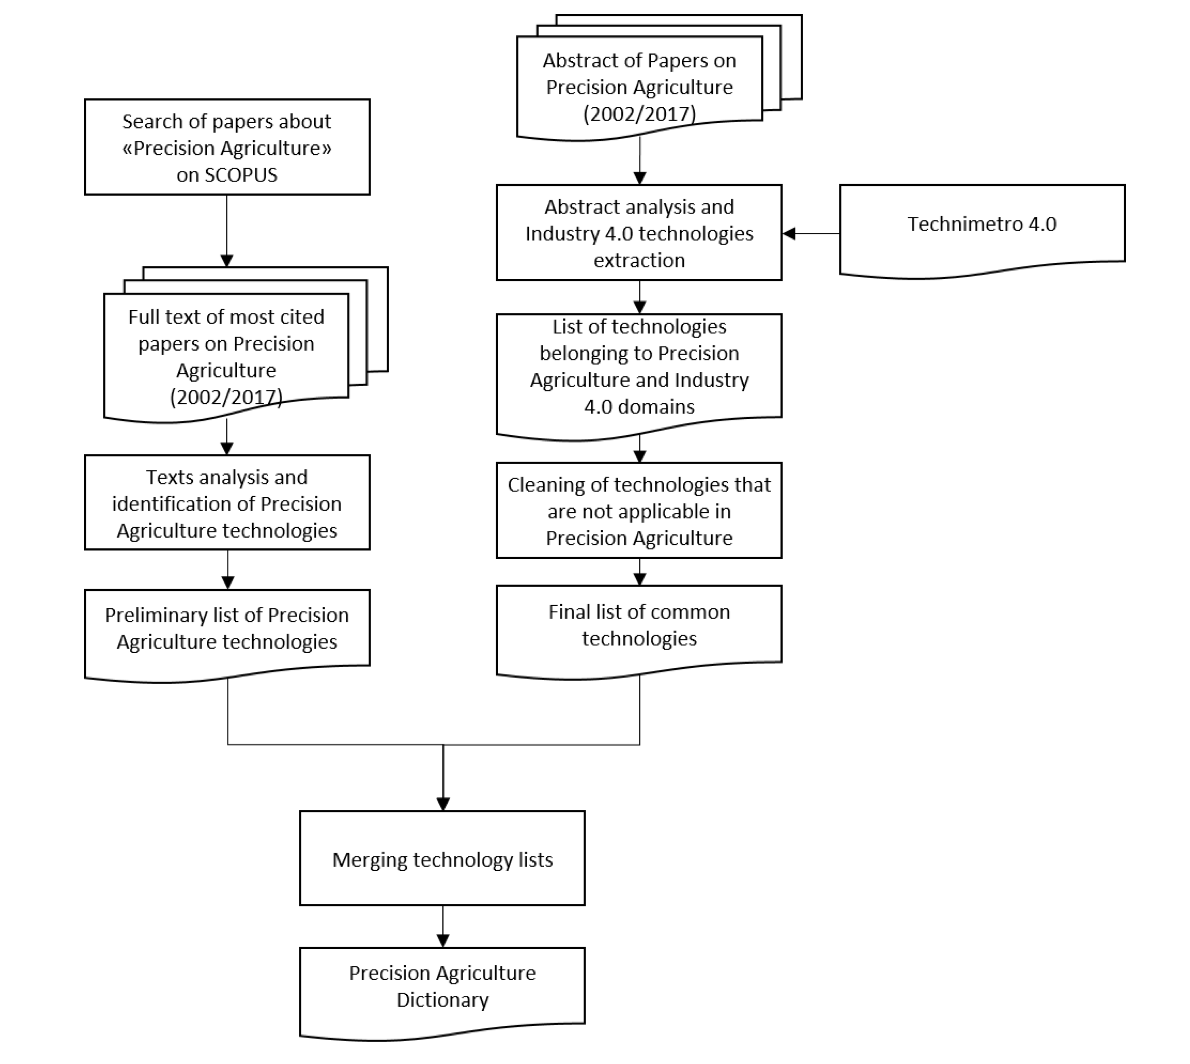
\includegraphics[width=0.8\linewidth]{_bookdown_files/figures/precisionwf} 

}

\caption{Process to create Precision Agriculture dictionary.}\label{fig:precisionwf}
\end{figure}

\subsection{Results}\label{results-6}

The dictionary of Precision Agricultural Technologies includes 324
terms. Thanks to a graph, the most cited technologies and the
connections between them allowed to identify at least 6 technology
clusters. The graph in Figure \ref{fig:precisiongraph} shows the
structure of the dictionary containing the technologies related to
Precision Agriculture and the relationships between the technologies
that compose it. This representation allows to deepen the connections
between the different clusters and technologies. The connections are
represented by the lines that join the different nodes (which represent
Precision Agriculture technologies) of the graph.

The size of the nodes varies proportionally to the number of papers they
are cited in, instead their position depends on the number of
connections between the different technologies: the most connected ones
acquire a more central position into the graph and vice versa. A sample
of the content of each cluster is:

\begin{itemize}
\item
  Monitoring: GPS, GIS, Data processing, GSM, Satellite, Ultrasound,
  Lidar, Broadband, Cellular, \ldots{}
\item
  IoT: Wireless sensor network, Internet of things, RFID, Bluetooth,
  Zigbee, Wi-fi, Microcontroller, Arduino, \ldots{}
\item
  Automation: Autonomous vehicle, Mobile Robot, Unmanned aerial vehicle,
  Agricultural robot, Computer vision, Data management, \ldots{}
\item
  Decision: Artificial intelligence, Data mining, Expert systems,
  Forecasting, Machine learning, Semantic web, Smart grid, \ldots{}
\item
  Hardware: Embedded system, Cyber-physical system, Manure spreader,
  Raspberry pi, CMOS, FPGA, \ldots{}
\item
  Laser: Laser, Laser transmitter, Laser receiver, Laser surveying,
  Optical fiber, Photonic sensor, \ldots{}
\end{itemize}

\begin{figure}

{\centering 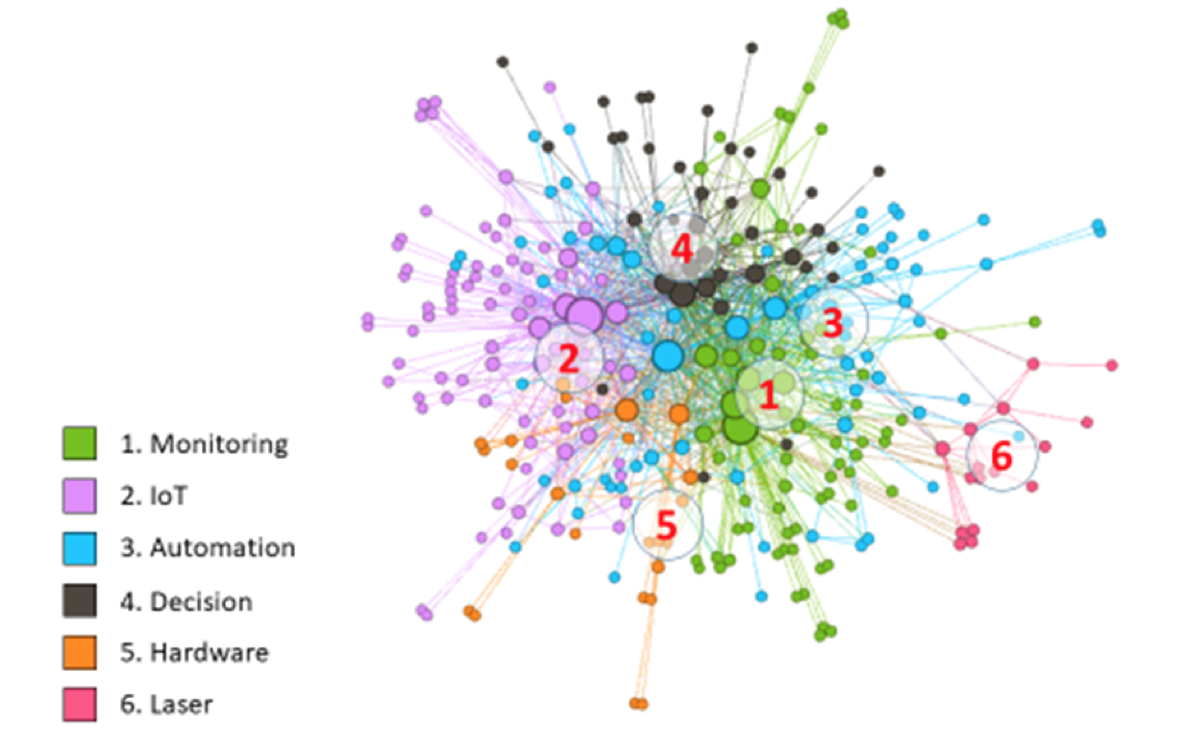
\includegraphics[width=0.8\linewidth]{_bookdown_files/figures/precisiongraph} 

}

\caption{Graph of the Precion Agriculture technologies.}\label{fig:precisiongraph}
\end{figure}

\chapter{Wikipedia}\label{wikipedia}

Wikipedia is a non-conventional source of technical knowledge, with
respect to patent and papers. With respect to the literature on field
delineation and clustering applied to science and technology we innovate
by introducing this new source. In particular in the present chapter,
Wikipedia is proposed as tool to map a technological field. The process
start with a small number of documents following a procedure which is
\emph{expert-independent}, in order to minimize the distortions from
subjective judgment. We then exploit the properties of Wikipedia in
order to delineate the field and identifying the linkages between
technologies. Further description of the structure of Wikipedia can be
found in section \ref{sotadocumentswiki}

In this section we present two methodologies capable of automatically
use Wikipedia information and its structure with the aim of mapping and
analysing this content. The results of the methodologies are described,
together with example of applications of the extracted entities for
intelligence tasks.

\section{Industry 4.0: Extracting and Mapping
Technologies}\label{technimetrochap}

Industry 4.0 is getting the center of the scene with respect to the
future of production systems in advanced countries and to its economic
and social implications. It is considered as the new fundamental
paradigm shift in industrial production. The new paradigm is based on
the advanced digitalization of factories, the Internet, and
future-oriented technologies bringing intelligence in devices, machines,
and systems \citep{lasi2014industry}. Despite its growing popularity and
the great expectations in terms of innovation impact, the concept of
Industry 4.0 remains strongly linked to technologies and frameworks that
have been heavily researched and analyzed in the last decades. In
particular, Industry 4.0 can be seen as a smart recombination of
existing technologies and some new technologies and their application to
the manufacturing environment \citep{trappey2016review}. This
recombinant nature has led some authors to claim that it is nothing more
than a re-labeling of old technologies, such as Computer Integrated
Manufacturing \citep{apreda2016functional}.

Yet other authors claim that this new wave of technology is
fundamentally different from previous technologies and not just an
amalgamation. In order to address the question whether Industry 4.0 is a
new paradigm, or rather a re-labeling of existing technologies, a
preliminary activity is needed, namely the delineation of the field and
the clustering of technologies covered in the perimeter. It turns out
that this activity is extremely challenging in the case of Industry 4.0,
for a number of reasons we discuss in great detail. Faced with the
complexity of Industry 4.0 existing delineation and clustering
methodologies can be considered inadequate.

In this section we develop a novel approach, test it, and show its
superior performance with respect to other approaches. The key features
of the approach are as follows:

\begin{enumerate}
\def\labelenumi{\roman{enumi})}
\item
  the description of Industry 4.0 is offered in the form of an
  ``enriched dictionary'', or an ordered and comprehensive collection of
  lemmas, each of which are associated to full scale definitions and
  descriptions and to explicit linkages to other lemmas;
\item
  the description of constituent technologies offered in the enriched
  dictionary is not obtained from individual experts, but is generated
  by accessing appropriate pages of the online encyclopedia Wikipedia;
\item
  the total number of technologies covered is more than 1200, linked
  with more than 39,000 semantic relations;
\item
  the perimeter of Industry 4.0 is not defined externally to the
  technology (by experts, government policies or other external sources)
  but is generated endogenously by examining the linkages between
  technologies described in the Wikipedia pages;
\item
  the update of the descriptions of technologies in the dictionary takes
  place in real time due to the distributed, parallel and selfcontrolled
  activities of authors in the worldwide community of contributors to
  Wikipedia;
\item
  new technologies are automatically included in the dictionary if they
  exhibit a given threshold of connectivity with those already included
  in the perimeter.
\end{enumerate}

\subsubsection*{Industry 4.0 as a multi-technology multi-stakeholder
field}\label{industry-4.0-as-a-multi-technology-multi-stakeholder-field}
\addcontentsline{toc}{subsubsection}{Industry 4.0 as a multi-technology
multi-stakeholder field}

Industry 4.0 is the main keyword used by researchers, policy makers and
entrepreneurs when describing how worldwide industrial systems will
evolve in the near future by leveraging Internet connected technologies
to generate new added value for organizations and society
\citep{roblek2016complex}. The growing interest is confirmed by the
increasing number of academic papers focusing on topics that are related
to the so-called ``Fourth Industrial Revolution''. As shown in Figure
\ref{fig:40trendscopus} the query ``Industry 4.0'' generates 967 papers.
Even if the query is very sharp and does not include all the research
efforts on the single ``enabling technology'' it demonstrates an
exponential growth of the topic. In Figure \ref{fig:40trendscopus} a
projection represented by the dotted line is included. The projection
has been drawn by considering a constant increase of the derivative
calculated as the average of the last 4 years. Our forecast is that in
2017 there will be 575 new papers in Scopus; this estimate is supported
by the fact that about 200 papers have been already published before
June 2017 (represented by the point). Since previous analyses in Scopus
demonstrate a delay between publication and loading of 5--6 months our
forecast seems to confirm a growing interest on the topic.

\begin{figure}

{\centering 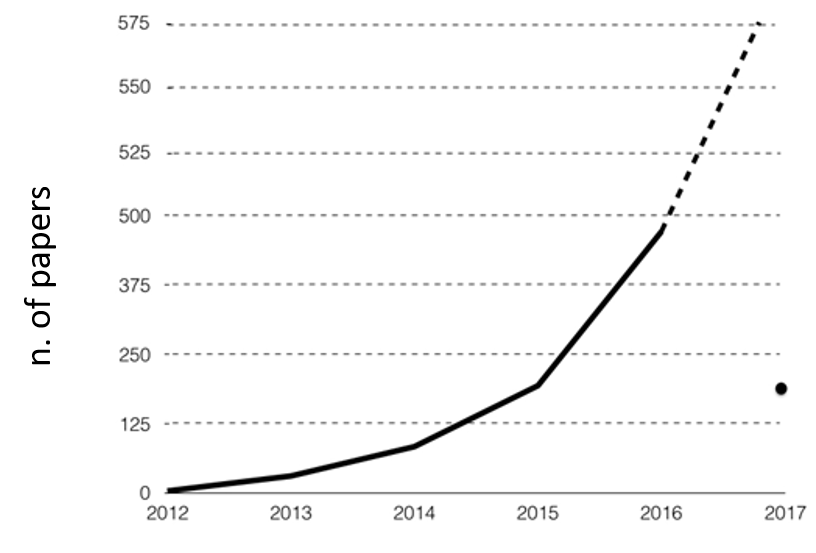
\includegraphics[width=0.6\linewidth]{_bookdown_files/figures/nofpapers190917} 

}

\caption{Trend of publications on Industry 4.0 (Title, Abstract, Keywords). Source: Scopus. Date: 06/06/2017}\label{fig:40trendscopus}
\end{figure}

Table \ref{tab:tabletech40scopus} shows how the scientific production on
Industry 4.0 is divided among the main research fields (multiple
attributions are possible in Scopus). In particular, it is possible to
identify field specific-technologies that refers just to one or few
sectors/business areas, and general purpose technologies that can be
exploited in several sectors/business areas.

\begin{table}

\caption{\label{tab:tabletech40scopus}Breakdown of industry 4.0 papers per research field. Source: SCOPUS date: 06/06/2017}
\centering
\begin{tabular}[t]{lr}
\toprule
Subject Area & Number of Publications\\
\midrule
Engineering & 645\\
Computer Science & 410\\
Business, Management and Accounting & 185\\
Decision Science & 134\\
Material Science & 90\\
\addlinespace
Mathematics & 87\\
Chemistry & 52\\
Physics And Astronomy & 45\\
Social Sciences & 34\\
Energy & 30\\
\bottomrule
\end{tabular}
\end{table}

Formulated initially in Germany in 2011, the Industry 4.0 paradigm has
been quickly translated, adapted and reinterpreted in developed and
developing countries.

Despite this rapid and impressive convergence of interest (in itself a
clear demonstration of the interdependence of policies across the
world), there is no common ground in the definition and delineation of
the field even if a first definition of the goal of industry 4.0 have
been presented since 1998 \citep{national1998visionary}.

More precisely, while there is a reasonable convergence on the
architectural definition of Industry 4.0, as defined in a relatively
loose way, there is still considerable disagreement and misalignment
with respect to constituent technologies
\citep{riel2017integrated, smit2016industry, o2015industrial}.

Furthermore, many constituent technologies are included in the
definition of Industry 4.0, and hence described in these documents, from
a variety of perspective that reflect mainly the huge variety of
application domains. In other words, technologies are often described
not only with respect to their fundamental engineering principles and
related dimensions of performance, but with respect to specific
applications to various manufacturing or service operations. In these
applications the specific working of technologies and the associated
dimensions of performance are indeed quite diverse.

Grangel and González \citep{grangel2016towards} develop a deductive
rule-based system able to identify conflicts among AutomationML
documents, named ALLIGATOR. It is interesting for the present work to
notice how ALLIGATOR has the function to interoperate and align
information models between a vast variety of areas (manufacturing,
security, logistics) at a micro/plant level. In other words, this paper
highlights the fact that one of the main problems of Industry 4.0 is the
integration of models and concepts typically developed in their
respective domains.

To offer an example of this state of affairs, let us consider the case
of RFID (Radio Frequency Identification and Detection) technology. One
of the main uses of RFID technology, that is, the detection of the
location of a tag moving along a known path with known speed can indeed
be applied for largely different purposes (safety, tracking,
localisation) and in various company areas (production, logistics,
maintenance). In practice, each of these applications will develop the
basic technology in different directions. Depending on the applications
we will find largely different descriptions of the technology involved.
Figure \ref{fig:techvaluechain40} offers a Value Chain-like
representation of Industry 4.0, showing the wide range of applications
of constituent technologies.

\begin{figure}

{\centering 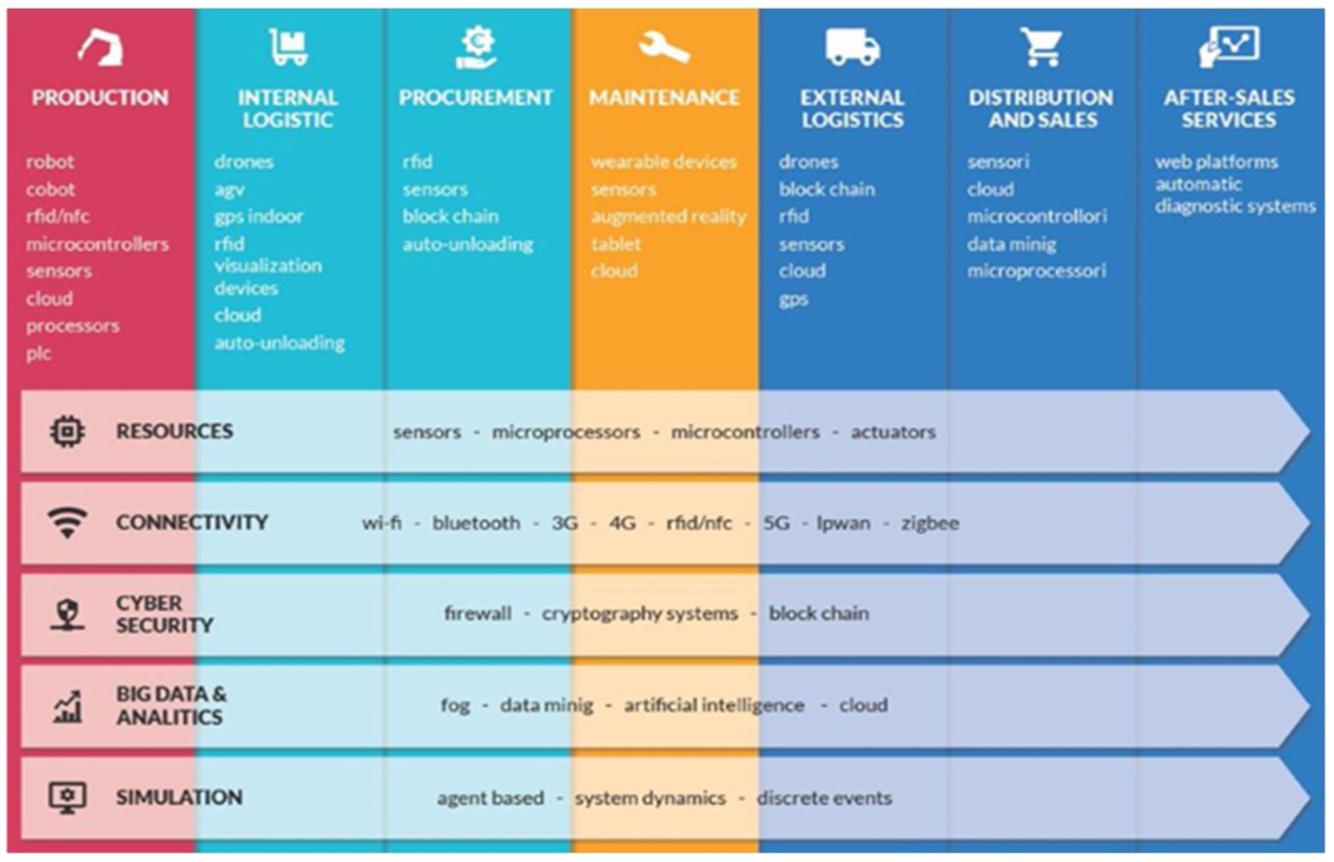
\includegraphics[width=0.7\linewidth]{_bookdown_files/figures/techvaluechain40} 

}

\caption{A Porter-like Value chain framework for Industry 4.0 (courtesy of Towel Publishing).}\label{fig:techvaluechain40}
\end{figure}

An interesting consequence of this state of affairs is that there is
disagreement also at the higher level of government documents describing
Industry 4.0 as the main object for innovation and industrial policies:
when describing the main components of Industry 4.0 the French
government uses 47 technologies, against 39 technologies for the Italian
government.

Summing up, the recombinant nature of Industry 4.0 creates several
interrelated problems for profiling and mapping: - the number of
constituent technologies is very large - the description and performance
of constituent technologies depend critically on the specific
application, hence on the business function/company area affected - the
stakeholders are located in several organizational positions - the
technical progress is very fast, with many (even if not all) constituent
technologies facing rapid changes in their nature and performance.

Faced with this situation, a traditional approach to profiling and
mapping would require a massive effort of keyword definition. A number
of experts would be recruited in order to offer a representation of the
field from their disciplinary or industry perspective. Extensive domain
knowledge would be mobilized in such a way to build up detailed yet
comprehensive maps of technologies. Based on these maps, governments,
statistical offices and international organizations would work for a few
years in line in the effort to identify the trends of technologies, the
most important actors, the shares of individual countries or regions in
the global landscape.

We strongly suggest this approach does not deliver the expected result.
Keyword-based approaches to emerging technologies are too dependent on
subjective judgments of experts. Even when the experts involved are top
class and disinterested (often the best researchers or industrialists),
their vision is inevitably partial. Even more importantly, keyword-based
representations cannot be updated with the same speed of technology. The
set of keywords identified by experts becomes inevitably obsolete in a
few months. This section leverages on publications and open source
repositories to design, develop and test a methodology that provides
delineation and clustering of technologies of the Industry 4.0 paradigm.
The methodology is based on a dictionary concerning the enabling
technologies for industry 4.0 with full definitions and connections
between them. Given the fast growth and the uncertainty that
characterizes industry 4.0 technologies, the present methodology is
designed to be a bottom-up and continuous evolving tool. The structure
and measurements made on the tool refer to July 2017.

\subsubsection*{Mapping and Clustering a complex emerging
technology}\label{mapping-and-clustering-a-complex-emerging-technology}
\addcontentsline{toc}{subsubsection}{Mapping and Clustering a complex
emerging technology}

The first task for mapping a new technology is field delineation, or the
definition of the perimeter of the field. Industry 4.0 is not a new
technology, but a novel combination of partly existing, partly new
technologies driven by the convergence of their trajectories. As a
matter of fact, it is clearly an example of emerging technology
\citep{rotolo2015emerging}, as it shares the features of rapid growth,
technological uncertainty, and market uncertainty.

The delineation of new fields of science and technology is an issue
addressed since the late `70s, after the pioneering period of
bibliometrics. Field delineation is a necessary step when existing
classifications do not offer timely, reliable or comprehensive coverage
of a topics, for example of a new technology or a new technological
field. Moving beyond existing classifications require undertaking a
search which, in general, may follow a lexical approach, a citationist
approach, or a mix between the two
\citep{small2006tracking, kreuchauff2017patent}. In all cases there is a
need to initialize the process, i.e.~to identify a set of elements that
constitute the starting point for searching.

The main approach has been based on keywords, to be identified in
various regions of documents (title, abstract, keywords, full text of an
article; title, abstract, claims, full text of a patent) and to be used
as queries. A query is a structured sequence of words, connected by
logical elements, such as ``or'', ``and'' and the like, to be launched
on a database in order to build up profiling, indexing, or clustering a
given field. In general the initial set of keywords are provided by
experts in the field, usually organized in an expert panel.

There are several limitations of the keyword/expert approach. First,
expert based keyword definition, or patent classification is a very
expensive activity \citep{tseng2007text}. Second, the keyword selection
is based on subjective judgment, and when experts are asked to decide on
relatedness measures (e.g.~synonims, hypernims or hyponims), they do not
apply systematic rules \citep[\citet{noh2015keyword}]{tseng2007text}.
Experts may be subject to a number of biases, such as for example the
desirability bias (attributing higher probability of occurrence to
preferred events) and many others (see section
\ref{sotadocumentsunderstandbyas}). Panels of experts are not immune by
biases, such as group thinking. There is little research on the impact
of expert subjective judgments on the delineation of emerging fields,
but there is reason to believe it may be significant.

Third, the delineation of perimeter of emerging technologies is not
robust to slight differences in the queries. As it has been shown by
Zitt and Bassecoulard, little differences in the wording of queries, or
on the time window, may end up in completely different sets of documents
\citep{zitt2006delineating}. Therefore there is no proof that the method
is reliable.

Finally, and more problematic for the case of Industry 4.0, the
methodology is static, as it is based on a fixed sets of words. This set
can (and in practice often is) updated, but this introduces a delay in
the process and does not deliver reliable results. Keeping updated a
collection of keywords in a dynamic technological landscape is extremely
difficult.

These limitations have become evident in the last two decades, after the
efforts of many authors to produce reliable perimeters of the emerging
field of Nanotechnology. The initial efforts have been based on a
classical expert-based approach. Panel of experts provided lists of
keywords that were transformed into database queries. Among them, a
consulting company called Lux, the Fraunhofer ISI in Germany, and CWTS
in the Netherlands were the most active. Most studies delivered largely
different delineations
\citep{youtie2008nanotechnology, ghazinoory2013application, ozcan2017patent}.

In turn, these limitations opened the way to massive efforts to reduce
the dependence on experts and exploit systematically the new
opportunities opened by text mining, following what has been called
``full text based scientometrics'' \citep{boyack2013improving}. Starting
from the late `90 s several attempts have been made to apply text mining
techniques to the patent corpus and the field is currently burgeoning
\citep{joung2017monitoring, ozcan2017patent}.

Summing up, the existing approaches to the delineation of emerging
technologies, taken together, suffer from the following limitations: 1.
dependence on expert judgment 2. lack of robustness to alternative
definitions of the perimeter 3. delay in update of technologies (static
approach) iv) lack of transparency in the modeling of technology.

We now turn to the second main task in text mining of technology
documents, that is, \emph{clustering}. Once the perimeter of the field
is delineated, a task usually included in the mapping is clustering, or
the creation of groups of entities in such a way to reduce the
complexity of the representation. Within text mining the clustering of
documents is based on various kinds of linkages that are considered a
signal of similarity in topics (see section
\ref{sotatoolsmodelnetanal}). In general, linkages among documents can
be generated by citations (citationbased clustering) or by the
extraction of features in texts (text-based clustering)
\citep{leydesdorff2006measuring, wang2017clustering, jaffe1993geographic}.

The most used approaches to clustering assume that members of a cluster:

-- cite each other (citation analysis:
\citep{jaffe1993geographic, moed2006citation, verspagen2007mapping, lee2017knowledge});

-- share certain words (co-word analysis:
\citep{callon1983translations, rip1984co, leydesdroff1989words, engelsman1994patent, van1993neural, yoon2004text});

-- share a reference in their bibliography (bibliographic coupling:
\citep{glanzel1996new, kuusi2007anticipating});

-- share the same sub-fields in a classification (co-subfield
analysis:\citep{chang2009using});

-- are cited by the same documents (co-citation analysis:
\citep{small1973co, small1985clustering});

-- are cited by the same authors (author co-citation analysis:
\citep{white1981author}).

In the proposed methodology we exploit the hyperlink feature of
Wikipedia in order to introduce a new approach to clustering. Hyperlinks
are introduced by authors in order to establish a semantic linkage
between the page and other pages. We exploit this feature as follows:
members of the same cluster are those pages that share the hyperlinks to
other pages, according to thresholds defined by an appropriate
algorithm. Note that hyperlinks are only superficially similar to
citations. The origin page cite another page by hyperlinking it, but in
effect this linkage is not a citation (that is, a reference to a
previous work) but a signal of semantic similarity, intended to guide
the reader in the network of meanings. We suggest that the hyperlinks
are similar to citations under some respect, but very different under
some other respects. Like citations, hyperlinks are introduced in the
text by authors and reflect intentionality. Unlike citations, they
reflect semantic relations, not relations of credit assignment or
tribute to scientific authority. Perhaps more importantly, citations are
introduced only by the author(s) of a paper and remain unchanged after
publication. Hyperlinks, on the contrary, are introduced also by
subsequent readers of the Wikipedia page. If the introduction of
hyperlinks is not considered appropriate by the community of
contributors, as it may happen due to vandalism, they are immediately
removed (see the discussion below). This means that they reflect all
possible semantic connections among the pages, as collectively stated by
a large community of authors, in a reliable and robust way. We believe
this methodology offers a remarkable improvement with respect to
existing approaches.

\subsubsection*{How is similarity measured by using
Wikipedia}\label{how-is-similarity-measured-by-using-wikipedia}
\addcontentsline{toc}{subsubsection}{How is similarity measured by using
Wikipedia}

In general, semantic relatedness is a measure of the similarity between
two terms. It can be computed by statistical methods without requiring a
manually encoded taxonomy, for example by analyzing term co-occurrence
in a large corpus \citep{resnik1999semantic, jiang1997semantic}.
Wikipedia has been largely exploited in the literature in order to
compute semantic relatedness. Gabrilovich and Markovitch
\citep{gabrilovich2007computing} developed an alternative to Latent
Semantic Analysis and called this new technique Explicit Semantic
Analysis (ESA). This methodology first uses a classifier that is
centroid-based to map input text to a vector of weighted Wikipedia
articles. Then the vectors are exploited to obtain the semantic
relatedness between two terms by computing the cosine similarity. This
technique could be applicable to individual words, phrases or even
entire documents. Furthermore, the mapping developed in this work has
been successfully utilized for documents categorization. A new version
of this kind of systems was presented by Milne
\citep{milne2007computing}. While in Gabrilovich and Markovitch
\citep{gabrilovich2007computing} the authors use the full text of
Wikipedia articles to establish relatedness between terms, in this work
only the internal hyperlinks are exploited. To compute the relatedness
between two terms, they are first mapped to corresponding Wikipedia
articles and then vectors are created containing the links to other
Wikipedia articles that occur in these articles. The main problem facing
semantic relatedness using Wikipedia is the disambiguation of terms.
Several strategies have been developed to solve this problem. A first
approach, described in Strube and Ponzetto \citep{strube2006wikirelate},
exploits the order in which entries occur in the disambiguation pages of
Wikipedia to find the most likely correct meaning. On the other hand,
Gabrilovich and Markovitch \citep{gabrilovich2007computing} avoids
disambiguation entirely by simultaneously associating a term with
several Wikipedia articles. Milne \citep{milne2007computing} approach
hinges upon correct mapping of terms to Wikipedia articles. However,
when terms are manually disambiguated, it has been shown that the
systems of semantic relatedness computation are more accurate than the
systems of automatic disambiguation \citep{medelyan2009mining}.

Summing up, a consistent literature in the field of computational
linguistics and text mining supports the notion that the use of
Wikipedia articles as a knowledge base is justified and promising.

\subsection{Methodology}\label{methodology-6}

In this section we give evidence of the methodological steps undertaken
to build up the enriched dictionary referred to Industry 4.0. The
dictionary contains technologies related to the Industry 4.0 paradigm,
each of which is associated to the full set of relations with other
technologies. The dictionary is semi-automatically generated using
technical documents and the Wikipedia free online encyclopedia. The
linkages between technologies have all a semantic content, since they
are generated within the text of the articles of Wikipedia when a
related topic or entry is considered necessary for the logical flow of
the definition or description.

Figure \ref{fig:wf40} shows the methodological steps needed to generate
the enriched dictionary. In the flow diagram three elements are
graphically displayed: activities (rectangular shape), check points
(diamond shape) and documents created from the procedure (sheet of paper
shape).

\begin{figure}

{\centering 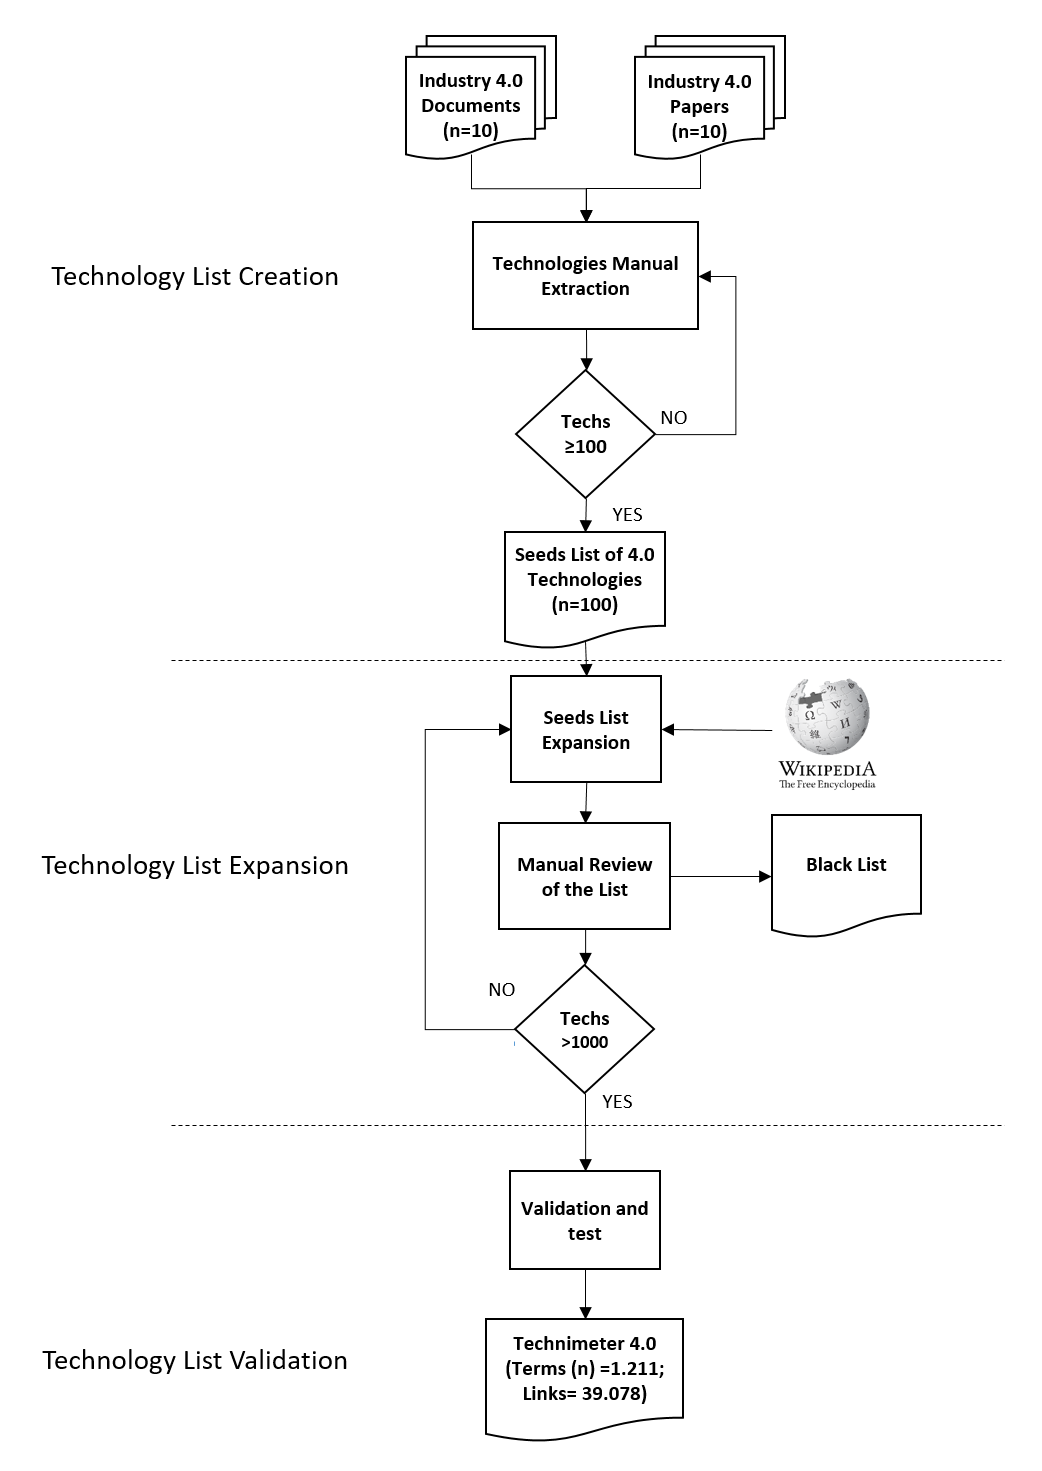
\includegraphics[width=0.8\linewidth]{_bookdown_files/figures/technimeter_03} 

}

\caption{Flow diagram of the adopeted methodology.}\label{fig:wf40}
\end{figure}

\subsubsection*{Generation of the seed
list}\label{generation-of-the-seed-list}
\addcontentsline{toc}{subsubsection}{Generation of the seed list}

As input for our methodology we used technical documents, official
government documents and the most cited academic papers in the field of
industry 4.0. The selection of seed documents has been made by:

-- taking the official government documents of the US government and of
three large European countries (France, Germany, UK), all of which are
strongly committed to the support of Industry 4.0 and are widely
considered a benchmark in international documents (for example, OECD and
European Union), plus a selection of technical documents cited in
government papers, for a total of 10 documents;

-- taking the 10 most cited papers on Industry 4.0 according to Scopus.
The reference to Industry 4.0 was explicit in the title, abstract and
keywords of the papers. The extraction was made on Scopus Database in
June 2017.

We deliberately limit ourselves to a small number of documents. The
reason is explained in conjunction with the chosen stopping rules. The
documents have been manually parsed by a team of Master students in
Engineering Management at the University of Pisa. The assignment was
``Understand each document and extract the enabling technologies for
industry 4.0''. The manual search in the documents continued until the
team reached the goal of 100 different technologies extracted. For our
purposes 100 different technologies represents a reasonable seed list of
technologies, which will be used as input for the automatic expansion
phase.

\subsubsection*{Seed list expansion}\label{seed-list-expansion}
\addcontentsline{toc}{subsubsection}{Seed list expansion}

For each term in the seed list the corresponding page in Wikipedia was
found. All technologies identified in the seed were covered by
Wikipedia. This is a preliminary confirmation of its relevance as a
source of knowledge. These pages formed the initial glossary. The
expansion procedure automatically retrieved the pages and identified all
hyperlinks included in the description of the technology. The pages that
are the target of hyperlinks are classified manually according to the
following categorization:

\begin{enumerate}
\def\labelenumi{\alph{enumi}.}
\tightlist
\item
  links to pages already in the seed: these pages are labeled
  ``anchors'', since they provide robust indicators of technologies that
  are, at the same time, mentioned explicitly in the seed documents and
  referred to in Wikipedia pages that deal with other technologies;
\item
  links to pages not in the seed: these are labeled ``missing
  technologies'' and are stored in memory for later treatment as
  potential candidates to inclusion in the dictionary;
\item
  links to pages with non-technological content: they are labeled
  ``stopwords'' and are eliminated from the procedure. The overall
  procedure is iterated up to the point in which a number of at least
  1000 different technologies is reached. At this point the procedure
  will stop. Updates and changes of the dictionary can originate from
  new entries (new technologies) or from updates to existing pages.
\end{enumerate}

Given that the automatic extraction of Wikipedia pages can be run on a
permanent basis, each version of the dictionary has a date. The current
version, illustrated in the rest of the paper, is at the time point of
July 15, 2017.

\subsubsection*{The stopping rule for the manual and the automatic
expansion}\label{the-stopping-rule-for-the-manual-and-the-automatic-expansion}
\addcontentsline{toc}{subsubsection}{The stopping rule for the manual
and the automatic expansion}

The three stopping rules follow a sequential logic of order of
magnitude: we start with approximately 101 documents, from which we
extract 102 names of technologies, that, used as inputs to Wikipedia,
deliver approximately 103 final technologies. More in detail we make use
of:

\begin{enumerate}
\def\labelenumi{\arabic{enumi}.}
\item
  20 input documents: all technical documents taken as reference for
  Industry 4.0 share the same framework (i.e.~DIN:SPEC 91345:2106). Many
  of the documents contains the same information/terms/ technologies.
  Furthermore these documents are technology focused and therefore from
  a low number of documents we obtain a large number of technologies.
\item
  seed list of 100 technologies: as demonstrated in the past Wikipedia
  is a good source also for technical terms, therefore we assumed it was
  able to quickly expand the technologies related to Industry 4.0. For
  this reason the seed list is composed of no more than 102 entries.
\item
  output list of at least 1000 technologies: of the automatic expansion
  works correctly the technologies should increase by an order of
  magnitude in few iterations. Since the list has to be revised manually
  we decided for 103 entries as a target thus reducing the impact of
  manual review. As a matter of fact, the Wikipedia network of semantic
  linkages delivers a total number of technologies related to Industry
  4.0 which exceeds this target, again confirming the validity of
  Wikipedia as a source of knowledge.
\end{enumerate}

\subsubsection*{Structure of the enriched
dictionary}\label{structure-of-the-enriched-dictionary}
\addcontentsline{toc}{subsubsection}{Structure of the enriched
dictionary}

The enriched dictionary can be defined as a set of enabling technologies
for industry 4.0, associated to their definitions and to the linkages
between them. The digital version of the tool is a hyperlinked text
\footnote{www.industria40senzaslogan.it}.

For the purpose of publication in an academic paper the tool can be
represented as a table in which we have:

\begin{itemize}
\tightlist
\item
  Column 1- Technologies: Enabling technologies for industry 4.0, or a
  broad categorisation of technologies following a clustering procedure
  (see below)
\item
  Column 2- Url: Links of the Wikipedia pages of the enabling
  technologies for industry 4.0
\item
  Column 3- Definitions: Glossary, snippets from wikipedia page of the
  definition of the enabling technologies for industry 4.0
\item
  Column 4 Links: hyperlinks to other wikipedia pages from the wikipedia
  pages of enabling technologies for industry 4.0
\item
  Column 5- Anchors: hyperlinks to other wikipedia pages that are
  enabling technologies for industry 4.0 from the wikipedia pages of
  enabling technologies for industry 4.
\end{itemize}

In the table shown in figure \ref{fig:technimetrosample} shows a sample
of the dictionary for four enabling technologies. An evidence is that
there are conflicting definitions of ``Augmented reality'' (AR) and
``Virtual reality'' (VR); the first says that AR contrasts VR, while the
second states that ``AR systems may also be considered a form of VR''.
This is an evidence of the ambiguity that exists in the definition of
4.0 technologies. Moreover, the table underlines how words such as ``3D
printing'' and ``Additive manufacturing'' that are used in different
ways within papers and technical documents (see Table 3), basically
refer to the same concept. Table \ref{fig:technimetrosample} also shows
the difference between links and anchors. Links include all hyperlinks
found in Wikipedia pages. By nature, a certain fraction of these links
contain information that is not relevant to our task. It is likely that,
in the course of discussion of a given topics, authors quote an author
(e.g.~Bob Sproull in Virtual Reality), an institution (e.g.~British
Museum or California Institute of Technology) or an event or application
(e.g.~Coachella Valley Music and Arts Festival). These links do not add
to our knowledge of the Industry 4.0 field. It can be seen that,
following the definition of anchor given above, these terms are
eliminated in column (E), which includes only the anchors, or those
entries that are added to the body of knowledge.

\begin{figure}

{\centering 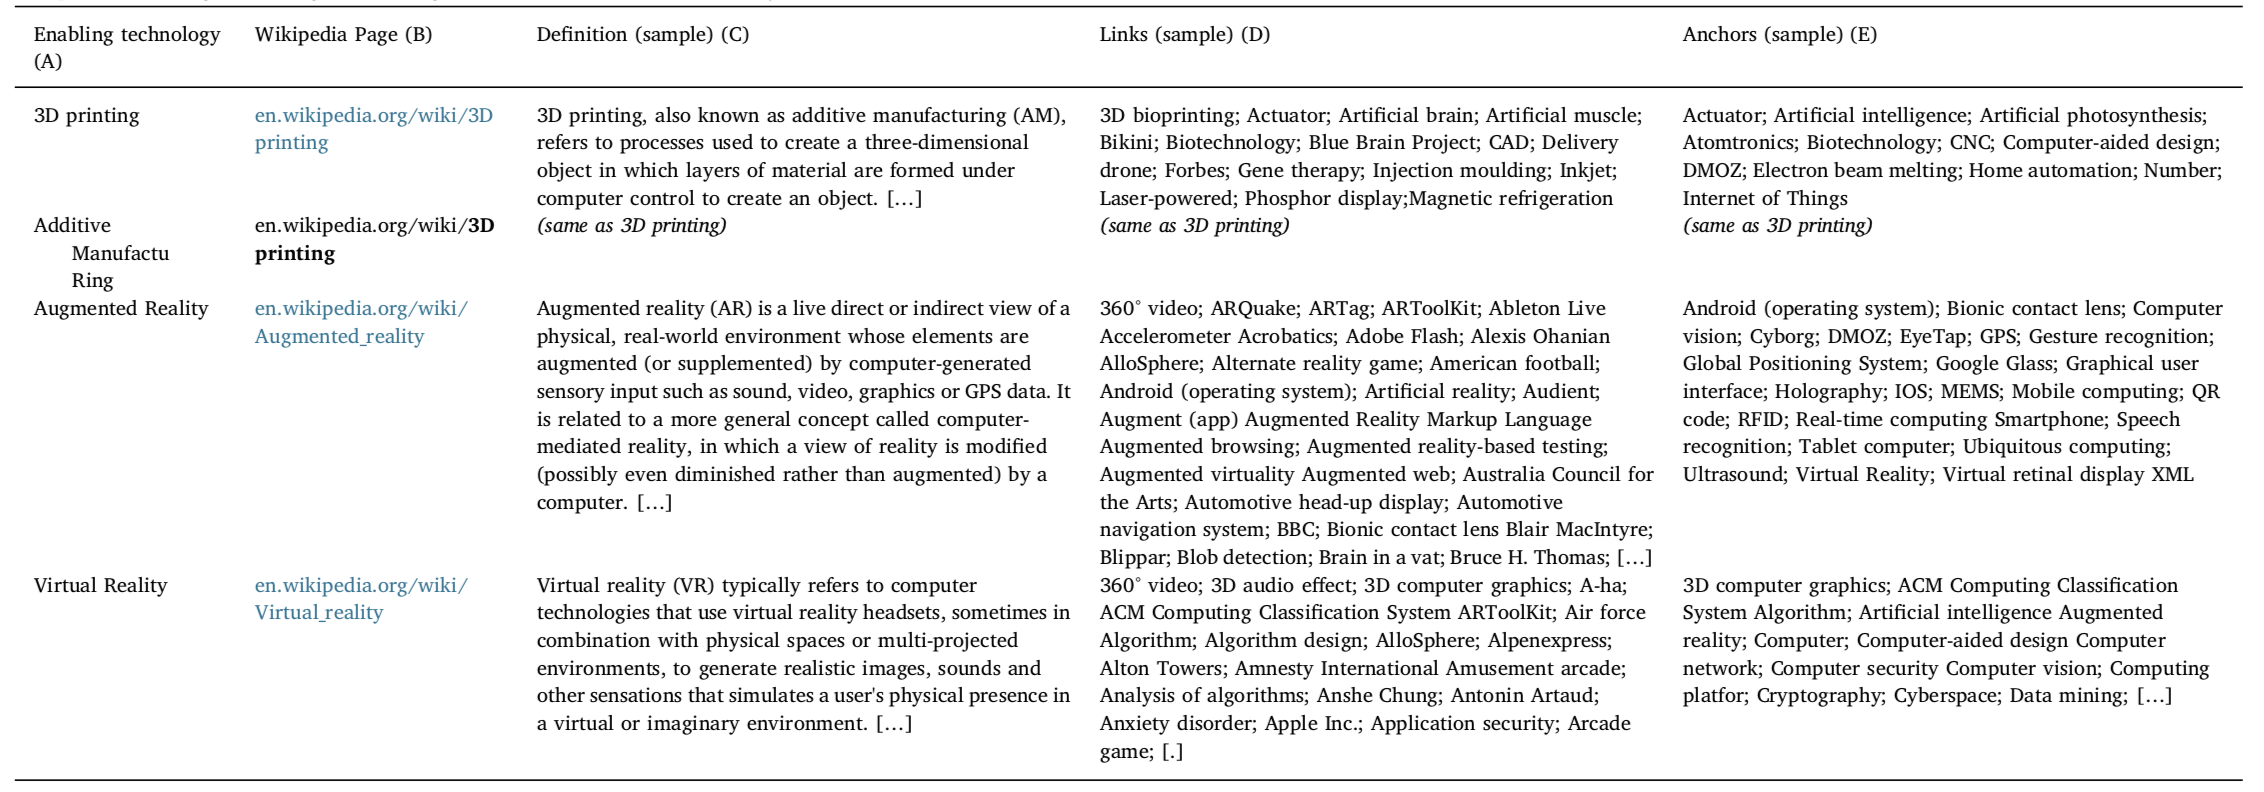
\includegraphics[width=1\linewidth]{_bookdown_files/figures/tabectechnim} 

}

\caption{Sample of enabling technologies showing the table structure of dictionary.}\label{fig:technimetrosample}
\end{figure}

\subsection{Results}\label{results-7}

The dictionary is composed of 1.211 terms and 39.078 relationships
between them. This generates a graph in which the node represents a
technology and the edge represents a link in the Wikipedia page. The
network structure naturally gives origin to graph-theoretic metrics. We
exploit this property in order to generate a number of indicators that
the readers may find it useful to examine.

\subsubsection*{Graph analysis and Sub-graph
selection}\label{graph-analysis-and-sub-graph-selection}
\addcontentsline{toc}{subsubsection}{Graph analysis and Sub-graph
selection}

Figure \ref{fig:techgraphplot1} gives an overview of the obtained. We
compute for each node the in-degree (horizontal axis), the out-degree
(vertical axis) and the number of links to other Wikipedia pages that
each node has (color of the node). Our results show that in terms of the
analyzed variables we can identify 4 different clusters of nodes (or
technologies) each one having a different behavior. The first group we
take in consideration are the point having an indegree greater than 70
and an out-degree greater than 70. In this group on the top right of the
page we have some outliers. These are terms like Microprocessor and
Microcontroller, X86, 8-bit, 16-bit and 32-bit. Then we observe a
sub-group centered on the coordinates (150, 100). Here we have terms
like Program counter, Adressing mode, Instruction Cycle, Coprocessor,
Symultaneus multitrading, SISD and MISD. Still within the first cluster
we have another sub-group of terms centered in (80,110) with terms like
Intel i860, Intel Atom, Intel 80286, Intel 80188 but also Bloomfiled and
Wolfdale. The second cluster is one in which the points have an
in-degree greater than 70 and an out-degree smaller than 70. Here we
have terms like Machine learning, Artificial Neural Network, Cognitive
Computing, Software, Random Access Memory, Internet, Firmware and C++.
The third group collects points having an in-degree lower than 70 and an
out-degree greater than 70. Here we have terms like Processors,
Micro-Operation, Micro-Assembler, Application specific integrated
circuit. The last and most populated cluster has an in-degree smaller
than 70 and an out degree smaller than 70.

\begin{figure}

{\centering 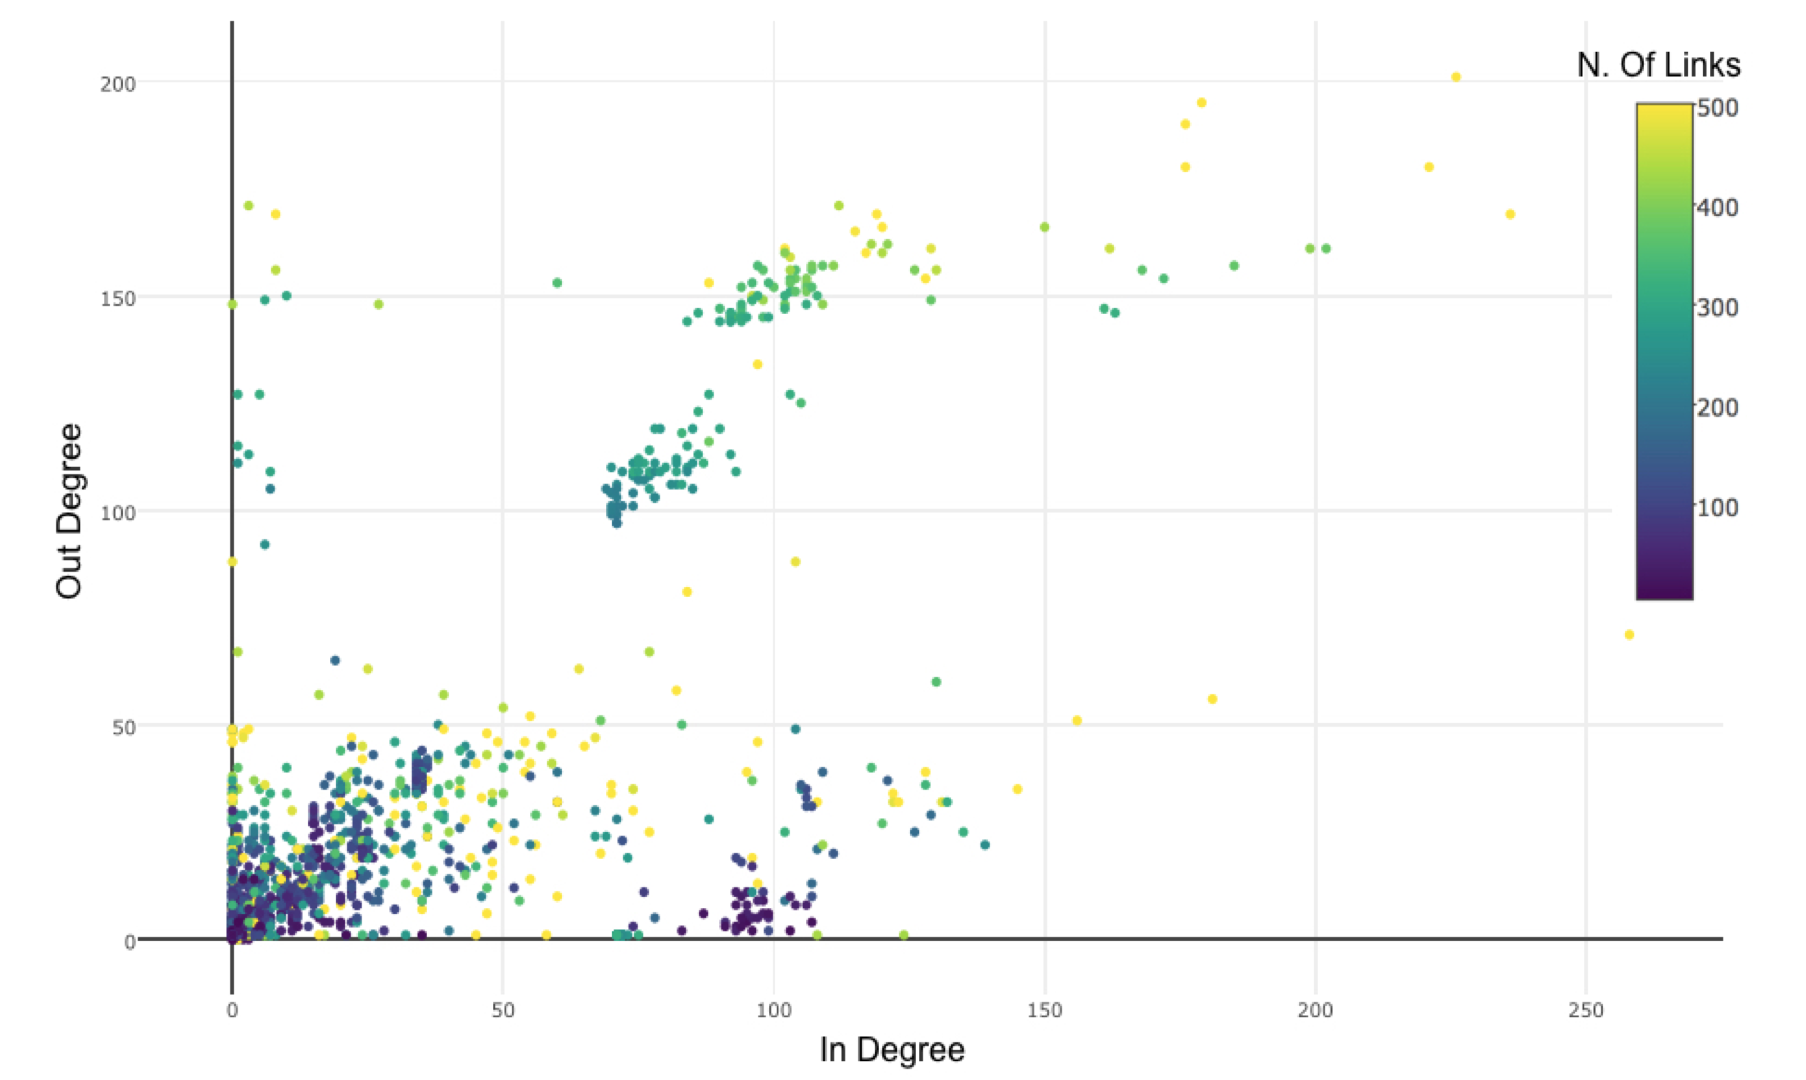
\includegraphics[width=1\linewidth]{_bookdown_files/figures/techgraphplot1} 

}

\caption{Plot of the in-degree and the out-degree of the nodes of the graph. The colour of the node represents the number of Wikipedia internal links.}\label{fig:techgraphplot1}
\end{figure}

This cluster is more precisely visualized in Figure
\ref{fig:techgraphplot2}, for which we have as before the in-degree
(horizontal axis), the out-degree (vertical axis) and the number of
links to other Wikipedia pages that each node has (color of the node). A
jitter process has been implemented to the points on the graph in order
to better visualize the overlapped points. In this plot only the
technologies having both an in-degree and an outdegree lower than 70 are
shown. This generates a subgraph composed by 931 nodes and 10673 edges.

\begin{figure}

{\centering 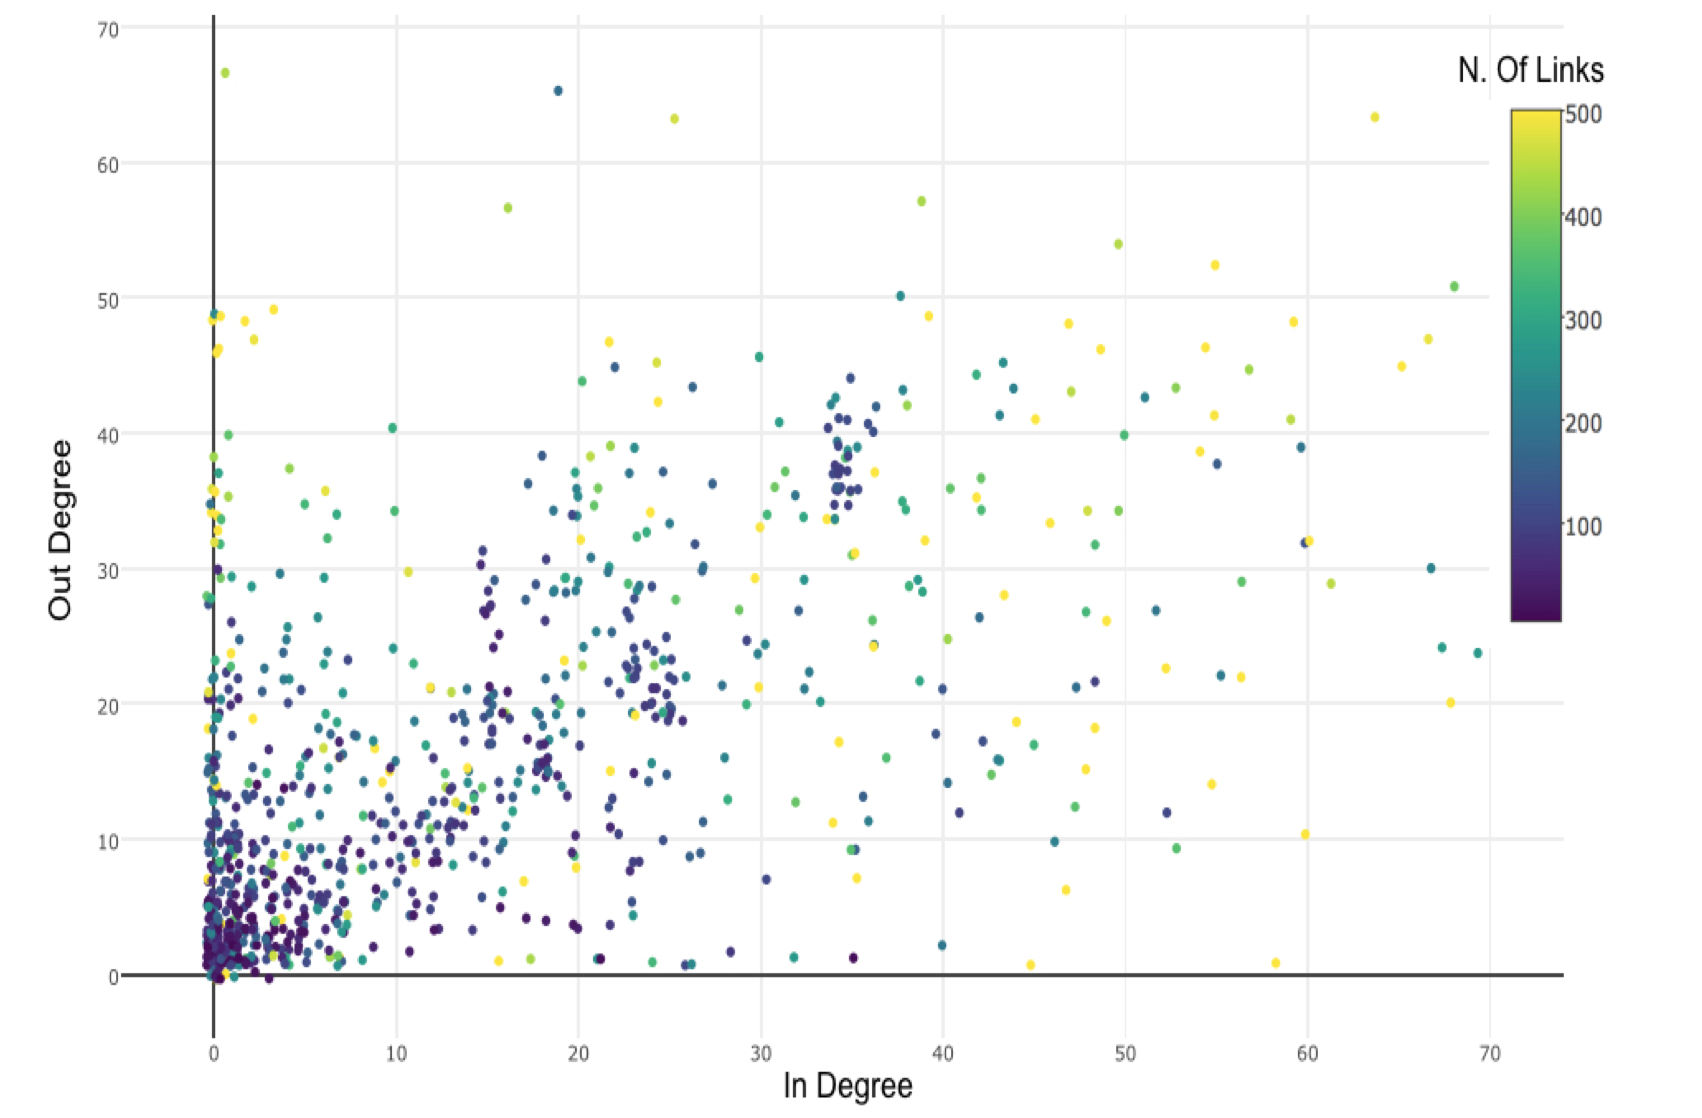
\includegraphics[width=1\linewidth]{_bookdown_files/figures/techgraphplot2} 

}

\caption{Plot of the in-degree and the out-degree of the nodes of the sub-graph. Selection of the nodes having an in-degree and an out-degree lower than 70. The colour of the node represent the number of Wikipedia internal links.}\label{fig:techgraphplot2}
\end{figure}

\subsubsection*{Graph representation and cluster
analysis}\label{graph-representation-and-cluster-analysis}
\addcontentsline{toc}{subsubsection}{Graph representation and cluster
analysis}

The structure of the graph offers it self naturally to clustering of
technologies in order to obtain a readable mapping. The clustering
algorithm receives as input the collection of technology terms T of the
analyzed subgraph and returns a set of terms clusters C = \{C1, C2,..,
Cn\} that cover the whole subgraph in analysis. Each cluster Ci is a
subset of terms of T, and a term may belong to only one cluster. In
Figure \ref{fig:technimetro} we show a representation of the sub-graph
made using Gephi software with its implementation of the Force Atlas
algorithm \citep{ICWSM09154} . In this representation, two nodes in the
graph are represented closely if they share an edge. In this way also
nodes that belongs to the same communities of nodes (nodes that can be
grouped into sets such that each set is densely connected internally)
but do not share any edge are represented closely. In other words, the
visualization tends to be coherent with the clustering algorithm. The
size of the node is proportional to its in-degree while the color
express the cluster to which each node belong. Finally some of the
labels of nodes and clusters are shown.

\begin{figure}

{\centering 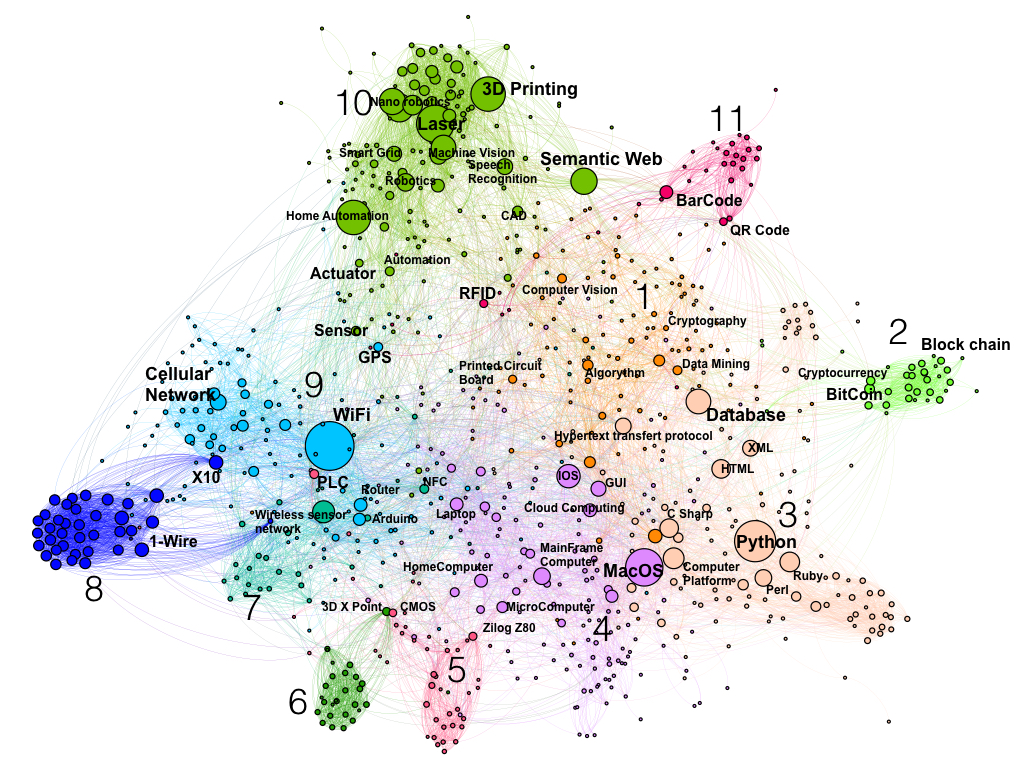
\includegraphics[width=1\linewidth]{_bookdown_files/figures/Graph_Tech.001} 

}

\caption{ Representation of the graph of 4.0 technologies and of the clusters in wich them are arranged.}\label{fig:technimetro}
\end{figure}

Each node is a technology and each edge represent a Wikipedia link
between the pages. The size of the nodes is proportional to the
in-degree, and the colors represent the clusters.

The algorithm we used to compute the modularity of each node and thus to
assign a group to each of them is described in Blondel et al.
\citep{blondel2008fast}. The process resulted in 11 clusters. The
content of each cluster is (for each cluster we can see the first 15
nodes in terms of in-degree):

\begin{enumerate}
\def\labelenumi{\arabic{enumi}.}
\item
  \emph{Big Data}: Virtual machine, Data mining, User interface,
  Algorithm, Computer vision, Cryptography, Printed circuit board,
  Middleware, Real-time computing, Virtual reality, Augmented reality,
  Human--computer interaction, Multiprocessing, Decision support system,
  Supervised learning
\item
  \emph{Transactions, digital certification, digital currency}: Bitcoin,
  Cryptocurrency, Bitcoin network, Cryptocurrency tumbler, Digital
  currency exchanger, Alternative currency, Dogecoin, Ethereum,
  Litecoin, Monero (cryptocurrency), Namecoin, Peercoin, Virtual
  currency, Auroracoin, Blockchain, Lisk, Primecoin, Ripple (payment
  protocol), Titcoin, Zerocoin
\item
  \emph{Programming languages}: Python (programming language), Database,
  Computing platform, Ruby (programming language), C Sharp (programming
  language), HTML, Perl, Hypertext Transfer Protocol, XML, Java
  (software platform), Haskell (programming language), .NET Framework,
  Lua (programming language), Sun Microsystems, BASIC
\item
  \emph{Computing}: MacOS, IOS, Mainframe computer, Graphical user
  interface, Cloud computing, Home computer, Laptop, Solaris (operating
  system), Microcomputer, Personal digital assistant, QNX, Read-only
  memory, Tablet computer, ASCII, DOS
\item
  \emph{Embedded Systems}: Programmable logic controller, Zilog Z80,
  CMOS, Zilog Z8, Toshiba TLCS, Zilog eZ80, NEC µPD780C, MOS Technology
  6502, R800 (CPU), U880, Zilog Z180, Zilog Z800, Zilog Z8000,
  КР1858ВМ1, Hitachi HD64180
\item
  \emph{Intel}: 3D XPoint, Intel ADX, Intel Clear Video, Intel SHA
  extensions, Intel System Development Kit, Intel 1103, Intel AZ210,
  Intel Cluster Ready, Intel Compute Stick, Intel Display Power Saving
  Technology, Intel Mobile Communications, Intel Modular Server System,
  Intel PRO/Wireless, Intel Quick Sync Video
\item
  \emph{Internet of Things}: Wireless sensor network, Near field
  communication, Arduino, NetSim, Z-Wave, OPNET, Telemetry, RIOT
  (operating system), Routing protocol, TinyOS, Internet of things,
  NesC, MiWi, Nano-RK, LinuxMCE
\item
  \emph{Protocols \& Architectures}: 1-Wire, Profibus, Smart meter, X10
  (industry standard), Modbus, Local Interconnect Network, TTEthernet,
  Fleet Management System, Keyword Protocol 2000, Meter-Bus, MTConnect,
  OPC Unified Architecture, PROFINET, RAPIEnet, SAE J1587
\item
  \emph{Communication Network and Infrastructures}: Wi-Fi, Cellular
  network, Router (computing), Internet Protocol, Radiotelephone,
  ARPANET, Radio frequency, Digital subscriber line, General Packet
  Radio Service, Global Positioning System, CYCLADES, Beacon, Wireless,
  High Speed Packet Access, Evolution-Data Optimized
\item
  \emph{Production}: Laser, 3D printing, Home automation, Agricultural
  robot, Nanorobotics, Semantic Web, Machine vision, Nanotechnology,
  Robotics, Information and communications technology, Speech
  recognition, Smart grid, Memristor, OLED, Computer-generated
  holography
\item
  \emph{Identification}: Barcode, RFID, QR code, MaxiCode, Mobile
  tagging, Code 128, GS1 DataBar, High Capacity Color Barcode, Aztec
  Code, Barcode printer, Bokode, Codabar, CPC Binary Barcode,
  Interleaved 2 of 5, ITF-14
\end{enumerate}

Let us examine more in depth a cluster, such as Identification (cluster
11). The size and colour of the words are proportional to the in-degree
of the nodes as shown in Figure \ref{fig:identificationspec}.

\begin{figure}

{\centering 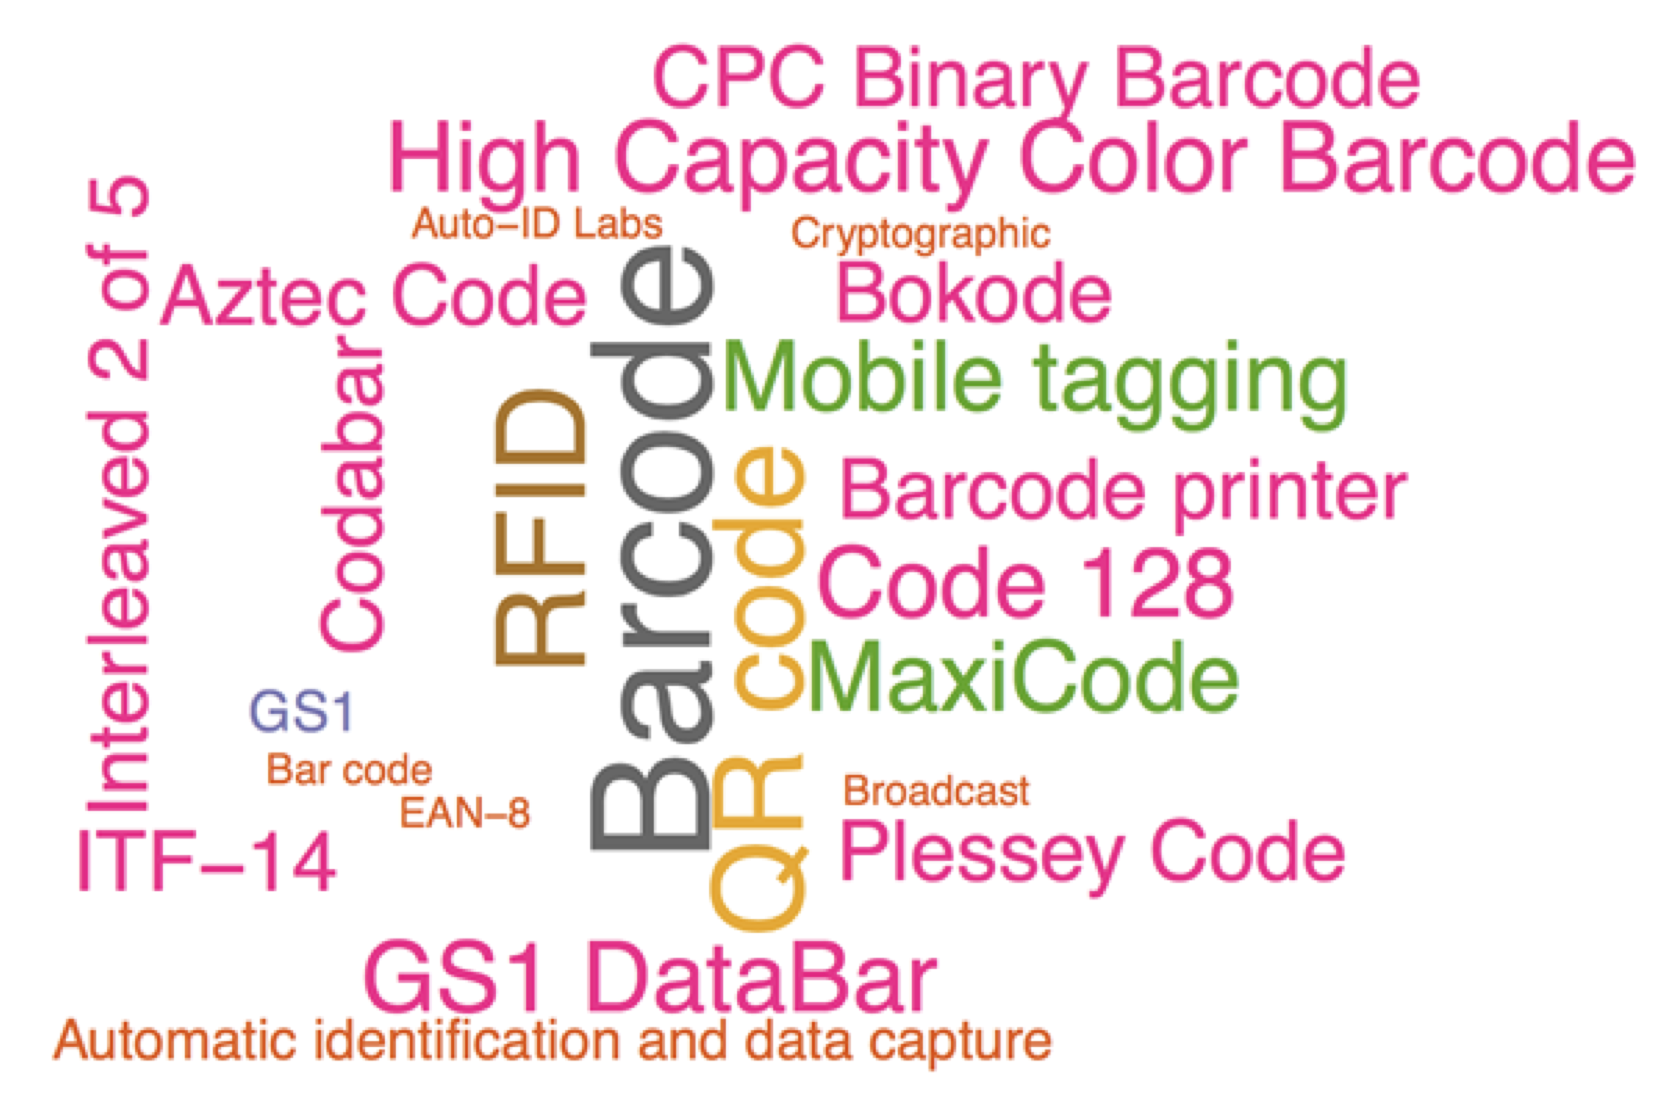
\includegraphics[width=0.7\linewidth]{_bookdown_files/figures/wctech} 

}

\caption{ Wordcloud of the words belonging to the class 11 labelled as Identification. In this figure the size is proportional to the logarithm of the in- degree of each node that represents a word.}\label{fig:identificationspec}
\end{figure}

\section{Industry 4.0: a Comparison with Industrie
4.0}\label{industry-4.0-a-comparison-with-industrie-4.0}

The Industry 4.0 paradigm can be understood and implemented differently
in different industrial eco-systems, depending on the country in which
it is adopted. In the present section we make use of Wikipedia to build
a network of pages regarding industry 4.0 in such a way that it is
possible to map how a country is actually implementing the industry 4.0
paradigm. To analyze the differences between the industry 4.0 concept in
the country of origin (Germany) and the rest of the world, our approach
is thus to investigate the Wikipedia pages of Industrie 4.0 and Industry
4.0 and the pages they are connected to. Using clustering algorithm it
is then possible to explore the different focus that countries have on
different technological sub-field of Industry 4.0.

All aspects during our analyses and the description of the project,
e.g.~page names, consist of two parts: one in English and one in German.
For simplicity and better understandability, we well mostly refer to
everything only by the English name.

\subsection{Methodology}\label{methodology-7}

In the present section we explain the methodology we adopted to build
and analyze the two graphs of Wikipedia pages representing the concepts
linked to industry 4.0 in Germany and in the rest of the world. As a
proxy of the world-wide vision of industry 4.0 we analyzed the English
version of Wikipedia. The main steps of our methods are represented in
the workflow of figure \ref{fig:industriewf} The first step consisted of
extracting all pages of interest from Wikipedia. Then the pages and
their connections were used to build two graphs (the German and English
version). The nodes of the graphs were then cleaned using a novel
approach based on the categories of the Wikipedia pages. Finally a
clustering algorithm was used to illustrate communities within the
graph. These steps are described in the following sections.

\begin{figure}

{\centering 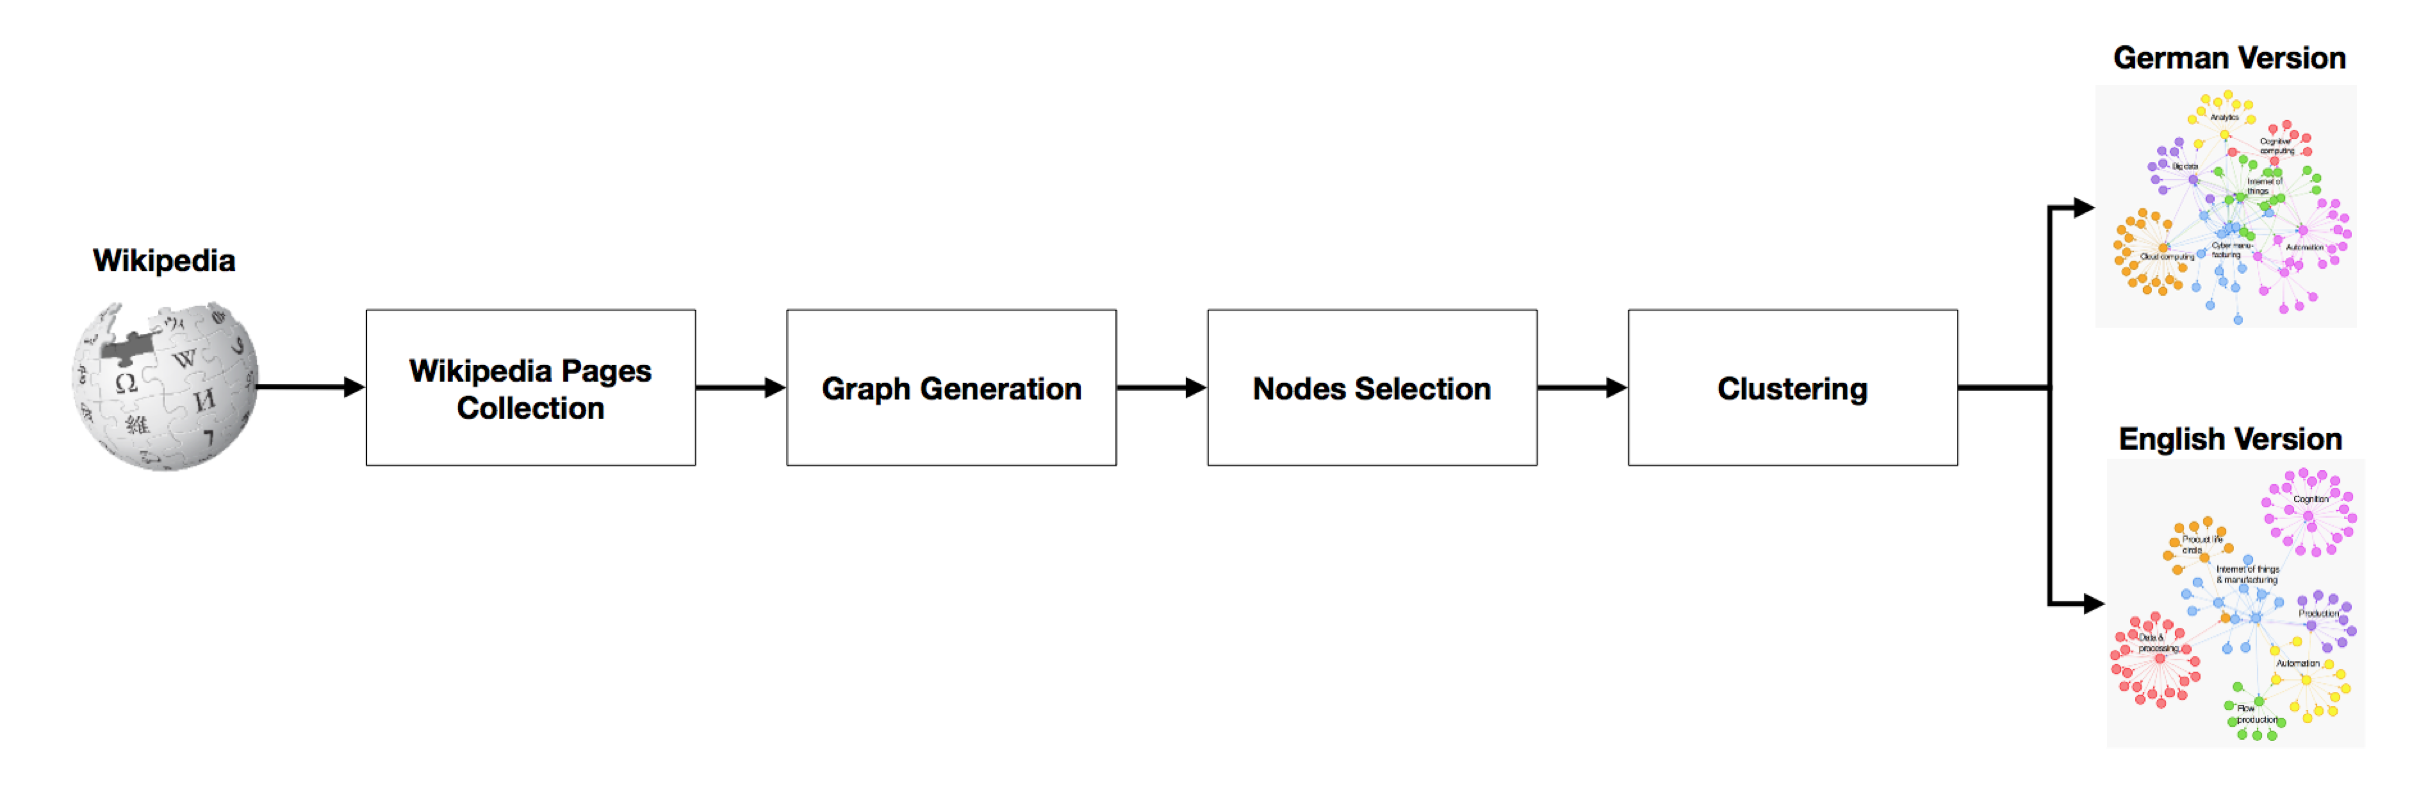
\includegraphics[width=1\linewidth]{_bookdown_files/figures/industrie_wf} 

}

\caption{The workflow shows the steps we followed to generate the two graphs of industry 4.0 related concepts.}\label{fig:industriewf}
\end{figure}

\subsubsection*{Wikipedia Pages
Collection}\label{wikipedia-pages-collection}
\addcontentsline{toc}{subsubsection}{Wikipedia Pages Collection}

To list the pages connected to the concept of Industry 4.0, all
Wikipedia pages that are linked to the page of Industry 4.0 (and
Industrie 4.0) were downloaded. We will refer to these pages as level 1
connection. Then all the pages linked to the level 1 pages are collected
and marked as level 2 pages. This process can be continued until a
wanted level is reached: for the purposes of the present work we decided
to show the effectiveness of the process stopping at level two. For each
page, we collected the links to other pages and the categories of the
page.

\subsubsection*{Graph Generation}\label{graph-generation}
\addcontentsline{toc}{subsubsection}{Graph Generation}

Two pages that are linked by a link within Wikipedia shares a certain
relations of which we ignore the meaning. Thus, it is possible that the
approach we described until now, also collects pages that are not
relevant for the analysis. In our case, this means that some of the
extracted pages are not technologically related to the subject of
Industry 4.0. Thus, the list of entries had to be cleaned from these
non-relevant ones. To make the filtering process more efficient, we
filtered considering the categories that had been extracted together
with the pages. We considered as relevant all the categories of the
pages of level 1. Then the level 2 pages were automatically considered
to be relevant if they were in one of the formerly marked categories.
For the nodes selection we also used a black-list of non-relevant
Wikipedia pages (e.g.~International Standard Name Identifier,
International Standard Book Number, Digital object identifier, ISBN),
previously developed by the authors in (see chapter
\ref{technimetrochap}). This list has been traduced in German for the
purposes of the present work.

\subsubsection*{Clustering}\label{clustering}
\addcontentsline{toc}{subsubsection}{Clustering}

In order to identify macro topics in the formerly created graphs, we
applied clustering methods. The most beneficial results were found to be
generated by applying a spin glass algorithm, which employs the spin
glass model and uses simulated annealing to find communities in networks
\citep{reichardt2006statistical}. In this approach the community
structure of the network is interpreted as the spin configuration that
minimizes the energy of the spin glass with the spin states being the
community indices.

\subsection{Results}\label{results-8}

In this section we will focus on describing the differences that emerges
between the two national technological approaches of industry 4.0 in
Germany and in the rest of the world.

\subsubsection*{The collected pages}\label{the-collected-pages}
\addcontentsline{toc}{subsubsection}{The collected pages}

We collect 97 pages for the German graph and 95 pages for the English
graph. A list of a sample of forty pages per language, alphabetically
ordered is:

\begin{itemize}
\item
  \textbf{German Version}: Absatzwirtschaft, Automatisierung,
  Automatisierungsgrad, Automatisierungstechnik, Autonomic Computing,
  Autopoiesis, Betriebswirtschaftslehre, Corporate Evolution,
  Cyber-physisches System, Dataset, Daten, Datenabgleich,
  Datenarchitektur, Datenaustausch, Datenbasis, Datenelement, Datenfeld,
  Datenmanagement, Datenmodell, Datenmodellierung, Datensicherung,
  Datenstruktur, Datentyp, Denken, Dienst (Informatik), Dienstleistung,
  Digitales Objektgedächtnis, Elektronische Datenverarbeitung,
  Erfahrungskurve, Erinnerungsvermögen, Feld (Datentyp), Feldgerät,
  Fertigungslinie, Fließbandabstimmung, Fließbandfertigung, Gegenwart,
  Geschichte der Produktionstechnik, Glauben, Gruppenfertigung,
  Halbzeug.
\item
  \textbf{English Version}: Adaptive system, Agent-assisted automation,
  Ambient intelligence, AmbieSense, Analytics, Artificial intelligence,
  Automated reasoning, Automation, Autonomic computing, Autonomous car,
  Big data, Big Data Maturity Model, Big memory, Carrier cloud,
  Cloud-based design and manufacturing, Cloud analytics, Cloud
  collaboration, Cloud computing, Cloud computing comparison, Cloud
  computing security, Cloud database, Cloud engineering, Cloud Foundry,
  Cloud management, Cloud manufacturing, Cloud research, Cognitive
  computer, Cognitive computing, Community cloud, Competitions and
  prizes in artificial intelligence, Computer-aided engineering,
  Computer-aided technologies, Computer-integrated manufacturing,
  Computer vision, Continuous analytics, Control loop, Control system,
  Cyber-physical system, Cyber manufacturing, Datafication.
\end{itemize}

\subsubsection*{The Graphs}\label{the-graphs}
\addcontentsline{toc}{subsubsection}{The Graphs}

The dimension of the graphs in terms of nodes, links and categories are
shown in Figure \ref{fig:graphmetricsindustrie}. From this figure is
evident how the two graphs has almost the same number of nodes; by the
way, the mean number of categories for the German version is close to
0.5 while its 0.3 for the English version. Beside these measure, as it
would be even more evident from further analysis, there is the broader
approach to industry 4.0 in the rest world with respect to the more
focused vision that Germany has.

\begin{figure}

{\centering 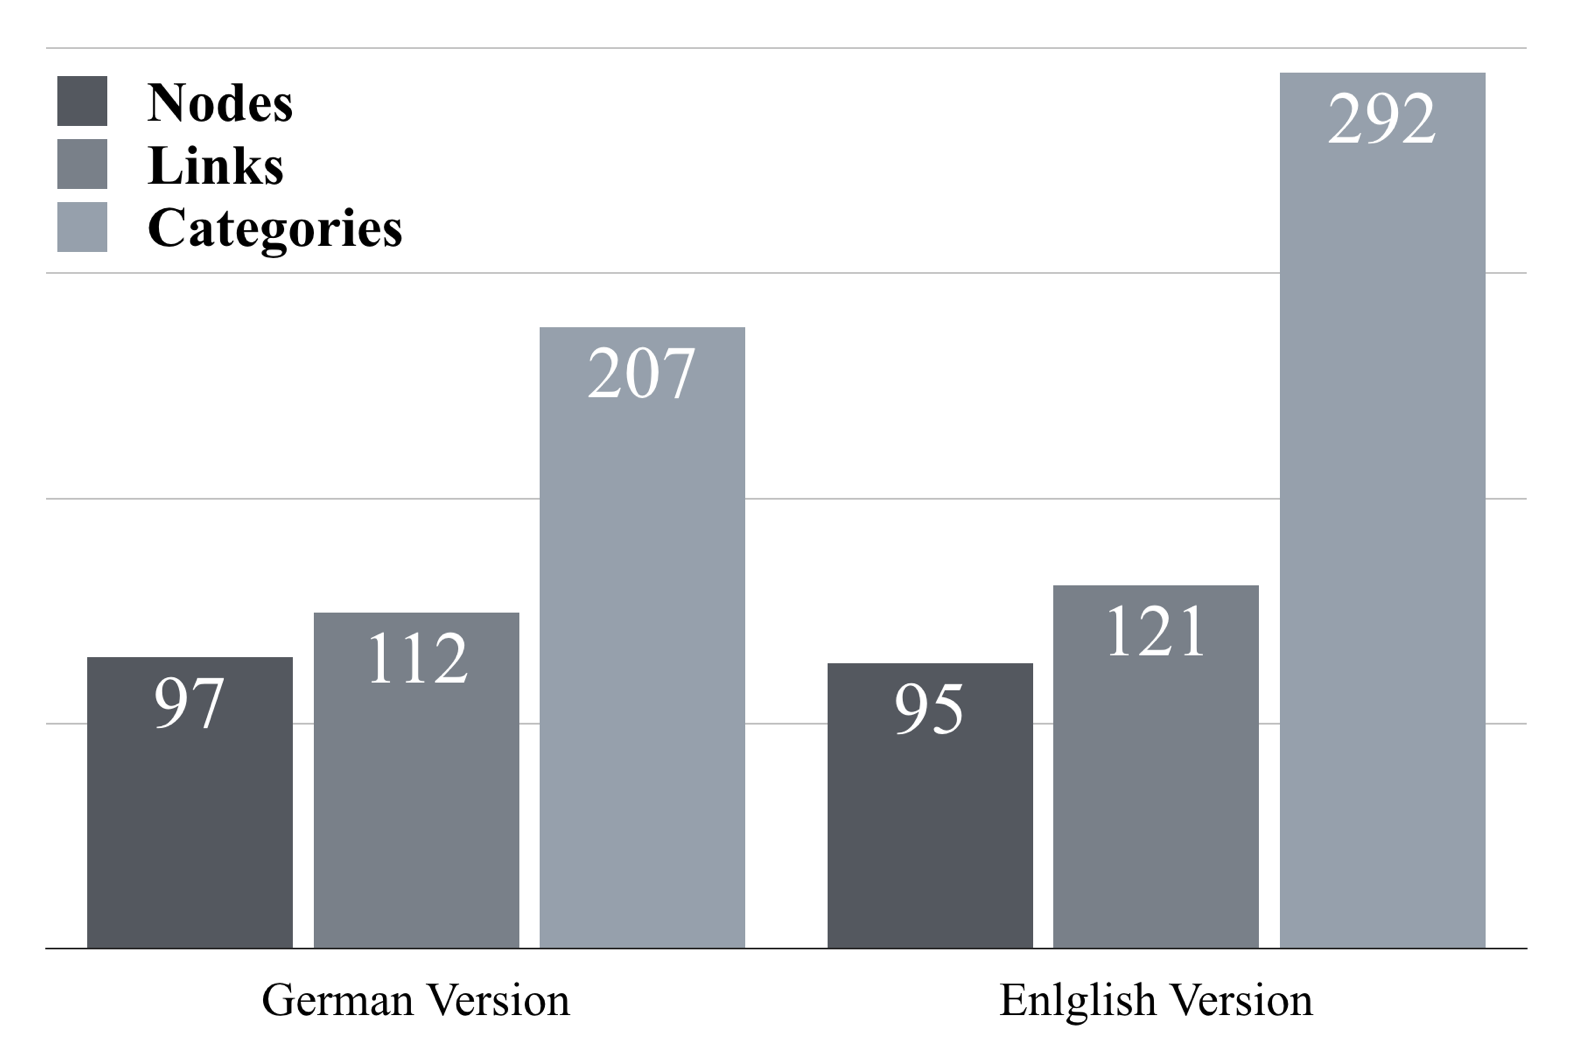
\includegraphics[width=0.8\linewidth]{_bookdown_files/figures/graph_metrics_industrie} 

}

\caption{Number of nodes, links and categories for the German version of the graph (left) and the English version (right)}\label{fig:graphmetricsindustrie}
\end{figure}

The resulting graphs are shown in figure \ref{fig:graphindustrie1}
(respectively the German version on the left and the English version on
the right). Here the vertices of the graphs represent the Wikipedia
entries, while the links are depicted by arcs that are directed from the
originating page to the linked page. The structures of the two graphs
and the difference in the number of links gives an evidence of the more
focused network of concepts in Germany: the number of links is in fact
lower for Germany, creating a more clustered graph.

\begin{figure}

{\centering 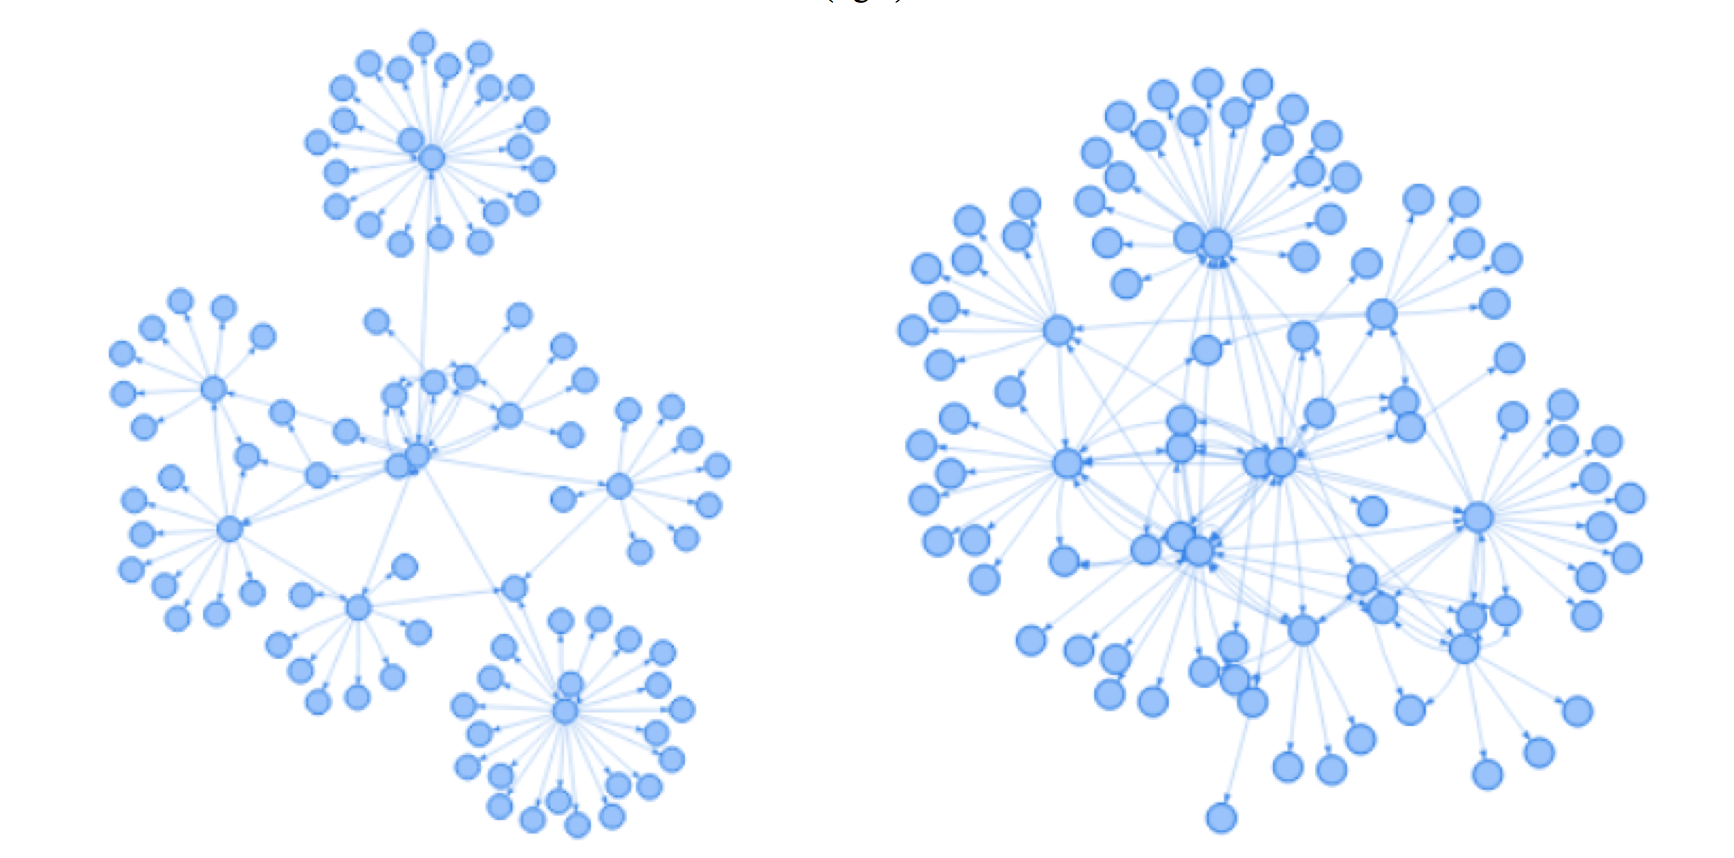
\includegraphics[width=1\linewidth]{_bookdown_files/figures/graph_1_industrie} 

}

\caption{The German version (left) and the English version (right) of the Industry 4.0 related graphs.}\label{fig:graphindustrie1}
\end{figure}

\subsubsection*{Graph metrics}\label{graph-metrics}
\addcontentsline{toc}{subsubsection}{Graph metrics}

In this section we analyze the graphs using standard metrics. These
measures allow investigations about relevant topology and specific
features of a given graph. More precisely, we looked at the following
measures: - Graph diameter: calculates the longest shortest path in a
graph, thus, the minimal distance between two nodes that are the
furthest away from each other. - Nodes Degree: Shows the number of nodes
that every node is connected to. The mean value of the degree for the
whole graph shows how interconnected the graph is: the higher the value,
the more connections the nodes have with each other. - Nodes Distance:
Gives back the minimum number of edges that connect one node with each
other. Here again, the mean value shows the interconnectivity of the
graph: A lower value means that the way from one node to another is
shorter, thus that the graph is more highly connected. The results of
these metrics for the two graphs are:

\begin{itemize}
\item
  German Version: Diameter= 4, Mean Degree= 2.38, Mean Distance= 3.25
\item
  English Version: Diameter= 4, Mean Degree= 3.29, Mean Distance= 3
\end{itemize}

From the diameter measure we can see that all of the pages are connected
through a maximum of 4 edges. This is not surprising, since it was a
premise of the method when setting the level to 2. Considering the mean
degree, a level of 2.38 for the German version and 3.29 for the English
version shows how the nodes of the English graph are more
interconnected. This can also be qualitative observed when looking at
the figures 3. Finally, the average distance from one node to another is
higher in the German graph, supporting the finding of the measures
discussed above.

These findings goes in line with what is said by a study of Acatech
\citep{kagermann2006industry}: in the USA, for example, the term
Industry 4.0 is understood in a much wider meaning. Furthermore, Acatech
study say that in Germany, the focus is mostly on technological
dimensions, while in the USA, the development of the new business models
in the area of big data analytics play a greater role, among others.

\subsubsection*{Clustering}\label{clustering-1}
\addcontentsline{toc}{subsubsection}{Clustering}

Figure \ref{fig:industrieclusters} shows the outcomes of the clustering
process: the vertices of the graphs represent the Wikipedia pages, the
links are depicted by arcs that are directed from the originating page
to the linked page and the clusters are represented by the different
colors of the nodes. In order to make these clusters comparable, the
label of the German version are translated in English. The resulting,
corresponding groups as well as the number of nodes they contain can be
found in table \ref{tab:industrietab3}.

Considering together figure \ref{fig:industrieclusters} and table
\ref{tab:industrietab3}, it is evident how the central node of the graph
(Industry 4.0) is contained in the first cluster Internet of things \&
manufacturing for both the graphs. It is also by design connected to all
other clusters, so that no cluster is isolated from Industry 4.0 node.

As evident from table \ref{tab:industrietab3}, the clusters in the two
graphs are similar. We have the same five clusters in both graphs and a
different one for each language. This shows that Industry 4.0 framework
if considered at a more abstract level, is similar in different
countries. This is not surprising, since there must be something that
made policy and industry call it the same name, but it is a strong
result for our methods, able to map bottom-up this phenomenon.

However, when looking at the clusters more closely, some interesting
differences get clear. The cluster production, product life circle \&
flow production, which is completely missing in the English graph, is
the one with the higher number of nodes in the German one. This shows
how the topic of Industry 4.0 in Germany is much more concentrated on
production than elsewhere. In the study of acatech
\citep{kagermann2006industry}, it is also explicitly stated that in
Germany `` {[}\ldots{}{]} the focus is on optimizing production
processes in terms of quality, price and flexibility and delivering
better financial returns overall''. The focus on production for Germany
is also confirmed by a monitor paper written by the by the European
Commission \citep{industrie2016eu}. To give a clearer view of this
phenomena, we have to consider that the word production is very similar
in meaning to manufacturing. The cluster including the latter (internet
of things \& manufacturing) has more than the double number of nodes in
the English graph with respect to the German one, so it might be that it
is rather the wording that makes the difference. Anyway, by looking at
the the disposition of the cluster (see figure
\ref{fig:industrieclusters}) internet of things \& manufacturing in the
two graphs, it can be observed that in the English version the cluster
is strongly integrated with ITC-related topics (Data processing \&
Analytics, Cognition and Cloud Computing), adding the adjective cyber to
the topic of manufacturing.

Additionally, also automation has more entries in the English version
and is highly connected not only to internet of things \& manufacturing,
but also to could computing, which does not even exist in the German
version of the graph: it is well known that Germany is not at the front
when it comes to the integration of ICT in Industry 4.0. This found is
again confirmed by the study of Acatech \citep{kagermann2006industry},
where it is said that ``Germany is currently lagging behind with regard
to data-driven business models and the development of large platform
ecosystems''.

The fact that cloud computing does not show up in the German graph is
examined more closely. In fact, a Wikipedia page about this topic does
exist in the German version of Wikipedia, but is not linked to the
Industrie 4.0 page. As stated in section 4.3, contributors of the German
version of Wikipedia tend to add only the most important connections
between pages. This again shows that integrated ICT is not the most
important topic in Germany now.

Another great difference in the number of nodes is in the cluster
cognition, which seems to be more important in the German version of the
graph. The German Wikipedia page describes this as a processing and
rearrangement of information between a human and a system. Acatech study
\citep{kagermann2006industry} does the same observation: ``In Germany in
particular, the focus is on integrating information, communication and
manufacturing technologies''. This could explain even better the finding
that the German graph lacks on the ICT side, giving a new
interpretation: in Germany there is a different interpretation of the
meaning of cognitive computing with respect to the rest of the world.

Finally, while the group of data, processing and analytics nearly has
the same amount of nodes, the links of this cluster with the other
clusters is quite different in the two graphs and also its content
changes from on nation to the other. Words like big data does not even
exist in the list of German pages related to industry 4.0 where it is
limited to just data. This emphasizes the careful approach of Germany
with this topic, which was also observed in \citep{wee2015industry}.
Germany seems to be rather conservative when it comes to new emerging
technological trends or even buzz-worlds like Big Data.

\begin{longtable}[]{@{}lll@{}}
\caption{\label{tab:industrietab3} Clusters names and number of nodes per
cluster for each version of the Industry Graph 4.0.}\tabularnewline
\toprule
Cluster & \# Nodes German & \# Nodes English\tabularnewline
\midrule
\endfirsthead
\toprule
Cluster & \# Nodes German & \# Nodes English\tabularnewline
\midrule
\endhead
1- Internet of things \& manufacturing & 12 & 28\tabularnewline
2- Cognition & 23 & 7\tabularnewline
3- Data, processing \& analytics & 23 & 19\tabularnewline
4- Automation & 12 & 20\tabularnewline
5- Cloud computing & - & 21\tabularnewline
6- Production, product life circle and flow production & 27 &
-\tabularnewline
\bottomrule
\end{longtable}

\begin{figure}

{\centering 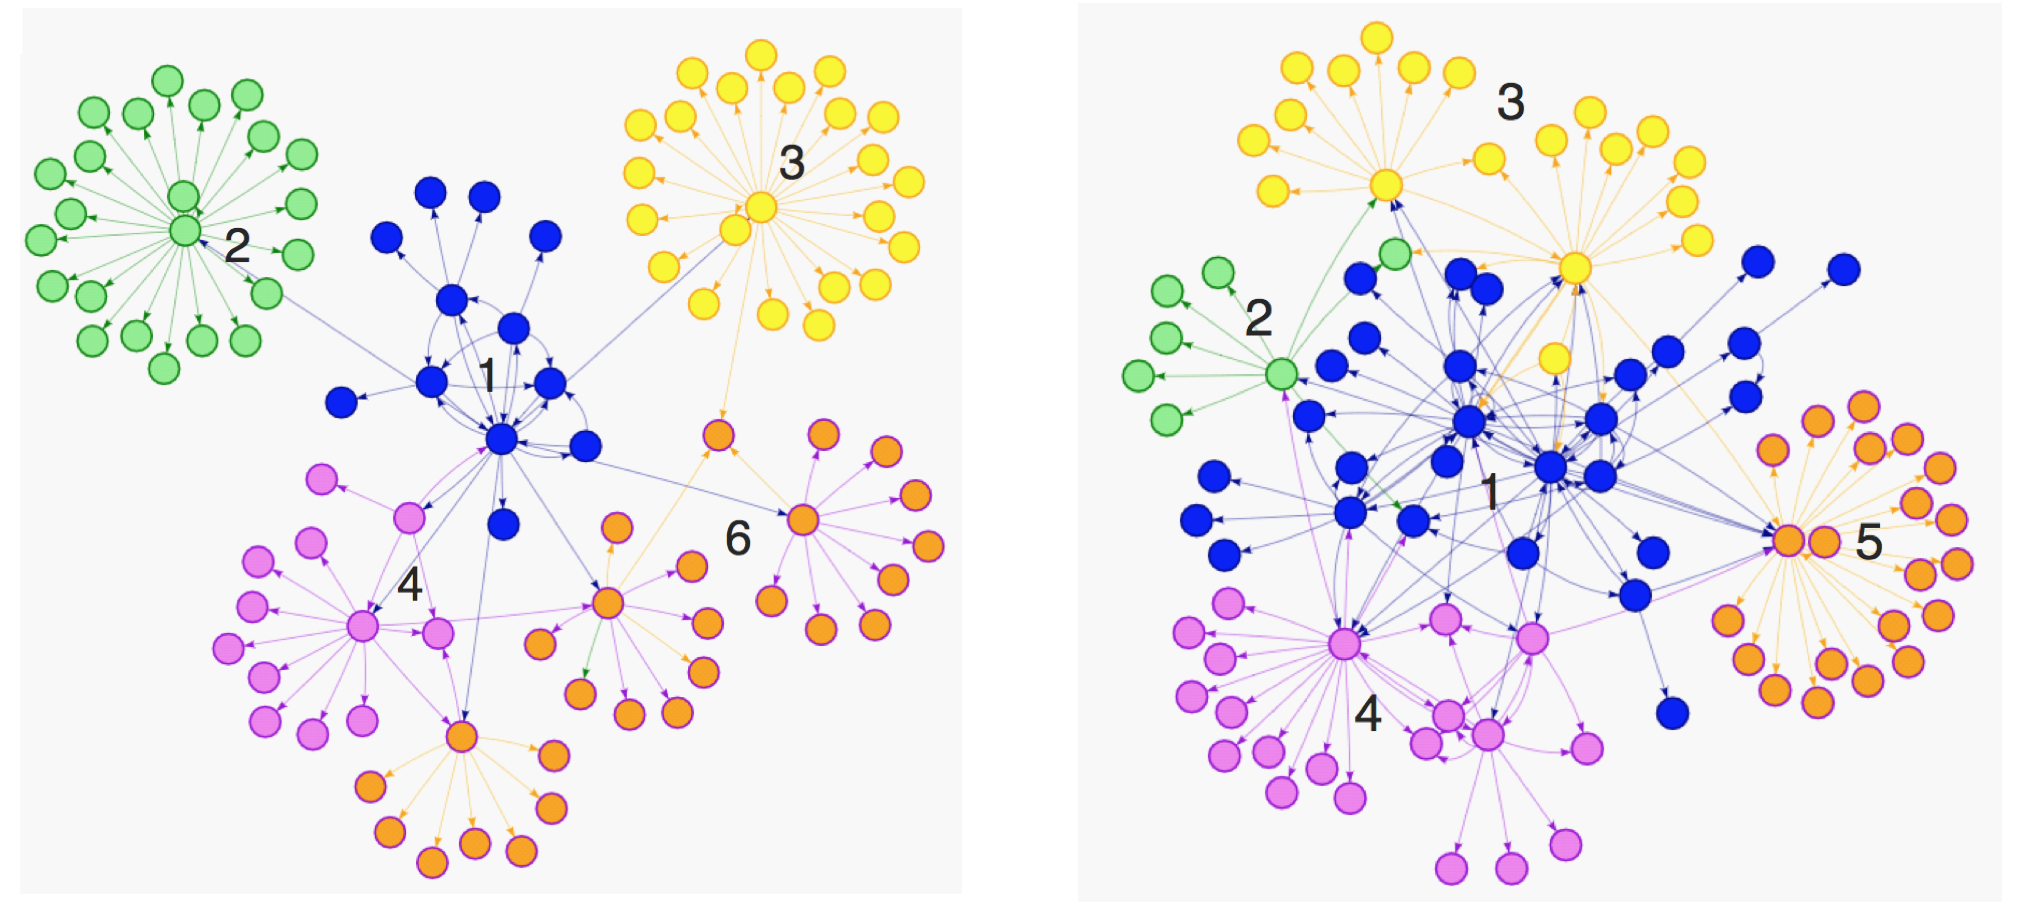
\includegraphics[width=1\linewidth]{_bookdown_files/figures/industrie_clusters} 

}

\caption{The German version (left) and the English version (right) of the Industry 4.0 clustered graphs.}\label{fig:industrieclusters}
\end{figure}

\chapter{Social Media}\label{social-media}

The technical knowledge generated by Social Media remains largely
untapped. Some researchers proved that social media have been a valuable
source to predict the future outcomes of some events such as box-office
movie revenues or political elections. Social media are nowadays also
used by companies to measure the sentiment of customers about their
brand and products.

This chapter proposes a new social media based model to measure how
users perceive new products from a technical point of view. This model
relies on the analysis of advantages and drawbacks of products, which
are both important aspects evaluated by consumers during the buying
decision process. This model is based on a lexicon developed in a
related work (see chapter \ref{advdrwresults}) to analyse patents and
detect advantages and drawbacks connected to a certain technology.

The results show that when a product has a certain technological
complexity and fuels a more technical debate, advantages and drawbacks
analysis is more efficient than sentiment analysis in producing
technical-functional judgments.

\section{Technical Sentiment Analysis}\label{techsentanal}

Nowadays, social media have become an inseparable part of modern life,
providing a vast record of mankind's everyday thoughts, feelings and
actions. For this reason, there has been an increasing interest in
research of exploiting social media as information source of knowledge
although extracting a valuable signal is not a trivial task since social
media data is noisy and must be filtered before proceeding with the
analysis. In this domain, sentiment analysis, which aims to determine
the sentiment content of a text unit, is considered one of the best data
mining method. It relies on different approaches
\citep{collomb2014study} and it has been used to answer research
questions in a variety of fields comprised the measure of customers
perception of new products \citep{mirtalaie2018extracting}. In this
section, we try to understand if sentiment analysis is really the best
available method to analyse consumer's perception of products,
especially when we want to measure the perception of the technical
content of the product. Thus we compare State of the art sentiment
analysis techniques with a lexicon of advantages and drawbacks related
to products.

\subsection{Methodology}\label{methodology-8}

Our work started with the selection of an event able to polarise Twitter
users' attention and products to analyse. In particular, we chose a
premiere tradeshow for the video game industry, and two video game
consoles disclosed during the event. We collected about 7 milions tweets
about products published before, during and after the tradeshow. Since
social media data is noisy (for example it may contains spam and
advertising), before proceeding with the analyses, we filtered our
dataset. In particular, after removing too short and non-English tweets,
we manually classified a randomly extracted subset of posts to train a
classifier which provide us the cleansed dataset. Then we conducted a
sentiment analysis of the tweets using state of the art machine learning
techniques. We classified each tweet as positive, negative or neutral.
At this point we applied our lexicon identifying advantages tweets and
drawbacks tweets. Finally we compared the outputs of the two analyses
for the two product-related clusters of tweets. We found consistent
differences between the extractions. The results shows that when a
product has a certain technological complexity and fuels a more
technical debate, advantages and drawbacks analysis is more able than
sentiment in producing technical-functional judgements. For this reason
we think that the proposed methodology peforms better then standard
sentiment analysis techniques when a product has a certain technological
complexity and fuels a more technical social media discourse.

\subsubsection*{Selection of a triggering event and
products}\label{selection-of-a-triggering-event-and-products}
\addcontentsline{toc}{subsubsection}{Selection of a triggering event and
products}

We chose the Electronic Entertainment Expo as event able to polarise
users' attention. Commonly referred to as E3, it is a premier trade
event for the video game industry, presented by the Entertainment
Software Association (ESA). We chose two new video game consoles,
disclosed at E3 2017, as products of which predicting the success or
failure. The first is Xbox One X, a new high-end version of Xbox One
with upgraded hardware and the other product is New Nintendo 2DS XL, a
streamlined version of the handheld console New Nintendo 3DS XL.

\subsubsection*{Data collection}\label{data-collection}
\addcontentsline{toc}{subsubsection}{Data collection}

Twitter provides two possible ways to gather tweets: the Streaming
Application Programming Interface (API) and the Search API. The first
one allows user to obtain real-time access to tweets from an input
query. The user first requests a connection to a stream of tweets from
the server. Then, the server opens a streaming connections and tweets
are streamed in as they occur, to the user. However, there are a few
limitations of the Streaming API. First, language is not specifiable,
resulting in a stream that contains tweets of all languages, including a
few non-Latin-based alphabets, that complicates further analysis.
Instead, Twitter Search API is a Representational State Transfer API
which allows users to request specific queries of recent tweets. It
allows filtering based on language, region, geolocation, and time.
Unfortunately, using the Search API is expensive and there is a rate
limit associated with the query. Because of these issues, we decided to
go with the Twitter Streaming API instead. For each product, we detected
related hashtags and keywords an constructed a query to download
relevant tweets. We chose to collect tweets not only after the
tradeshow, but also before. For these reason, we initially identified
some products keywords with their provisional names and we updated them
at a later stage. Tweets have been downloaded from CNR (Consiglio
Nazionale delle Ricerche, Istituto di Informatica e Telematica, Area di
Pisa) since 11th June 2017 h. 10:00 to 31th July 2017 h. 15:00.

\subsubsection*{Data filtering}\label{data-filtering}
\addcontentsline{toc}{subsubsection}{Data filtering}

The initial dataset resulted to be very noisy, containing tweets written
in different languages, advertising and posts related to different
products or subjects. We chose to keep into account only English tweets
because sentiment and advantages/drawbacks lexicon is in this language.
The data set is filtered removing tweets with less than five words and
non-English posts with a language classifier. We obtained 7.165.216 of
filtered tweets.\\
At this point we created a golden set of relevant tweet to train a
Supported Vector Machine classifier able to recognize relevant and
unrelevant tweets. We defined characteristics that make a tweet: (i)
relevant (posted by users or containing words or opinions related to our
products of interests and their functionalities), (ii) irrelevant
(tweets containing advertisings, links to e-commerce websites or
messages related to other products or subjects). A researcher manually
classified a subset made up of randomly extracted tweets. In particular,
we extract a subset composed of 6.500 finding 105 positive results and
6.395 negative. SVM model was then trained using this dataset, and
computed a probability for each tweet to be relevant or irrelevant. A
threshold of 0.7 has been chosen to label a tweet as relevant. The final
dataset of filtered tweets, made up of 66.796 posts. We clustered tweets
using product-related keywords. Clustering posts allowed us to further
filter the final dataset which contained a small number of irrelevant
tweets (Table \ref{tab:tweetab1}).

\begin{longtable}[]{@{}lrr@{}}
\caption{\label{tab:tweetab1} Clusters of tweets.}\tabularnewline
\toprule
& N° of tweets & \% of tweets\tabularnewline
\midrule
\endfirsthead
\toprule
& N° of tweets & \% of tweets\tabularnewline
\midrule
\endhead
Xbox One X & 64885 & 0.9714\tabularnewline
New N2DS & 1706 & 0.0255\tabularnewline
Irrelevant tweets & 198 & 0.0030\tabularnewline
\bottomrule
\end{longtable}

\subsubsection*{Sentiment analysis}\label{sentiment-analysis}
\addcontentsline{toc}{subsubsection}{Sentiment analysis}

Table \ref{tab:tweetab2} presents the results of the sentiment analysis.
We classified each tweet according to its sentiment into positive,
negative, or neutral. We used an established methodology developed by
\citep{cimino2014linguistically}. We pre-processed the tweets by
removing mentions (@ character), URLs, product hashtags, emoticons and
single characters. As a result, for each tweet we obtained a probability
of belonging to a mood class. After a manual analysis, we used a class
prediction probability threshold of 0.6 to filter out low confidence
prediction, i.e.~tweets that cannot be classified as positive or
negative with a high confidence are classified as neutral instead.

\begin{longtable}[]{@{}lrrr@{}}
\caption{\label{tab:tweetab2} Clusters of tweets.}\tabularnewline
\toprule
& Positive & Negative & Neutral\tabularnewline
\midrule
\endfirsthead
\toprule
& Positive & Negative & Neutral\tabularnewline
\midrule
\endhead
Xbox One X & 0.3599 & 0.0465 & 0.5937\tabularnewline
New N2DS & 0.5299 & 0.0158 & 0.4543\tabularnewline
Overall & 0.3642 & 0.0457 & 0.5901\tabularnewline
\bottomrule
\end{longtable}

\subsubsection*{Advantages and drawbacks
analysis}\label{advantages-and-drawbacks-analysis}
\addcontentsline{toc}{subsubsection}{Advantages and drawbacks analysis}

To extract technical advantages and drawbacks from tweets we used the
lexicon developed in chapter \ref{advdrwresults} that contains 657
Advantages words and 297 Drawbacks clues. These words are searched on
our dataset finding different percentages of tweets with words from the
lexicon in the two product-related clusters of tweets. Table
\ref{tab:tweetab3} reports the results.

\begin{longtable}[]{@{}lrrrrr@{}}
\caption{\label{tab:tweetab3} Percentages of tweets containing or not words
from our lexicon.}\tabularnewline
\toprule
& Adv & Drw & Adv \& Drw & No Adv or Drw & Adv or Drw\tabularnewline
\midrule
\endfirsthead
\toprule
& Adv & Drw & Adv \& Drw & No Adv or Drw & Adv or Drw\tabularnewline
\midrule
\endhead
Xbox One X & 0.0884 & 0.0374 & 0.0037 & 0.8705 & 0.1295\tabularnewline
New N2DS XL & 0.0662 & 0.0094 & 0.0000 & 0.9244 & 0.0756\tabularnewline
\bottomrule
\end{longtable}

\subsection{Results}\label{results-9}

We adapted the advantages \& drawbacks analysis to give as output a
classification of each tweet. We classified data coming from the latter
analysis in this way:

\begin{enumerate}
\def\labelenumi{\arabic{enumi}.}
\tightlist
\item
  positive (tweets containing only advantages words)
\item
  negative (tweets containing only drawbacks)
\item
  neutral (tweets with no words of our lexicon or controversial tweets)
\end{enumerate}

As we can see in figure \ref{fig:tweetsentres}, sentiment analysis is
more able to polarise tweets. In fact, with this analysis we found lower
levels of neutral tweets, respectively 59.37 \% for Xbox One X and
45.43\% for the New Nintendo 2DS XL.

\begin{figure}

{\centering 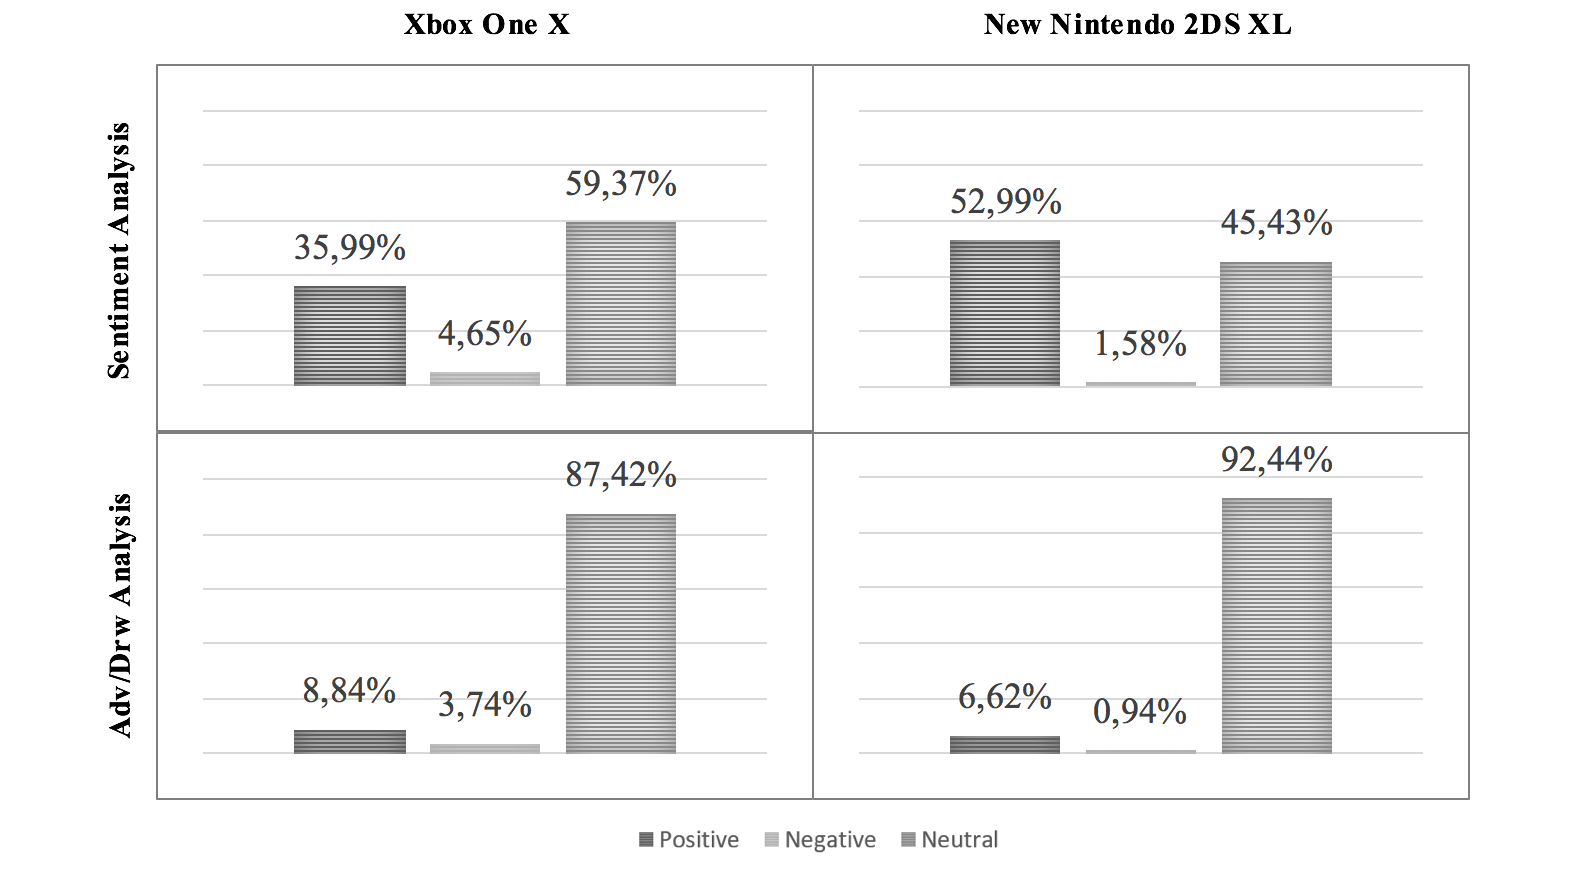
\includegraphics[width=1\linewidth]{_bookdown_files/figures/tweet_sent_res} 

}

\caption{Comparison between Sentiment analysis and Advantages/Drawbacks analysis.}\label{fig:tweetsentres}
\end{figure}

This was an expected result since this kind of analysis is designed to
deal with colloquial language while our lexicon is technical, being
derived from patents analysis. What surprised us is the different
polarisation of the products that we see comparing the two analyses. In
fact, while with sentiment analysis Nintendo achieves lower percentages
of neutral tweets, with advantages and drawbacks analysis is the
opposite, since Xbox tweets are more polarised. We also noted that we
found more tweets with words of our lexicon in the Xbox subset than in
the Nintendo one (\ref{tab:tweetab3}). We did the hypothesis that the
differences between the percentages of tweets with words found for each
product, and the differences of polarisation between the two analyses
depend on the different marketing focus, target customer, and
technological complexity of the two new video game consoles. Xbox One X
targets hard-core gamers who really wants a premium experience
\footnote{\url{http://www.businessinsider.com/why-xbox-one-x-costs-500-2017-6?IR=T}
  (last access: 17/11/2017)}. With its marketing campaign, Microsoft
pushed the technical supremacy of its new machine over the competitors'
products, fuelling a debate about its technical features amongst the
potential users.

As a result, the campaign produced a more technical social discourse
that allowed us achieving better results. Instead, the new Nintendo
handheld console has been developed targeting children and families
providing a model that falls somewhere in the middle of the line of 3DS
consoles \footnote{\url{http://www.nintendolife.com/news/2017/05/reggie_explains_the_reasoning_behind_the_new_2ds_xl}
  (last access: 17/11/2017)}. We initially checked our hypothesis using
Google Trend to compare users' search interest about technical review of
the two products during the data collection period (Figure
\ref{fig:tweetsearchinterest}). Then, we analysed the number of
technical articles related to the new products published by the 25 most
popular video games and technology websites in the U.S, according to the
ranking of SimilarWeb, a digital marketing intelligence company which
publishes insights about websites. We used Google search engine to
retrieve technical article within the web domains previously identified:
we obtained 1.117 articles about Xbox and only 52 about Nintendo,
proving that technical debate concerning Xbox is greater. This is and
evidence of the fact that when a product has a certain technological
complexity and fuels a more technical debate, advantages and drawbacks
analysis is more able than sentiment in producing technical-functional
judgements. The greater number of neutral tweets found with advantages
and drawbacks analysis can also be explained with the Means-end chain
model \citep{reynolds1995means}. Consumers express themselves basing on
personal consequences linked with product use or basing on personal
values satisfied by the product itself. For these reasons, tweets
contain a more colloquial language which sentiment analysis is more able
to interpret than the latter tool.

\begin{figure}

{\centering 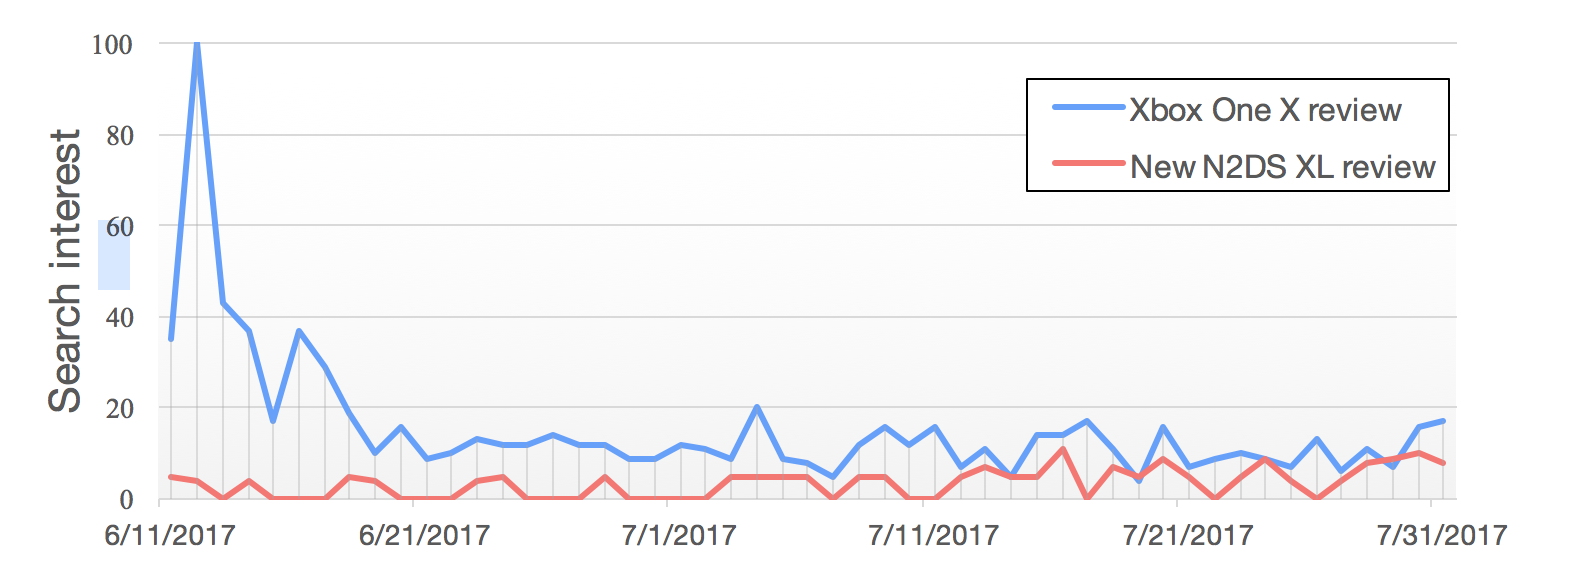
\includegraphics[width=1\linewidth]{_bookdown_files/figures/tweet_search_interest} 

}

\caption{Google Trends comparison of search-terms “Xbox One X review” and “New Nintendo 2DS XL review” during the data collection period, since 11th June 2017 to 31st July 2017. Values on the vertical axis depict search interest compared to the highest point in the graph during the observation time. A value of 100 is the peak popularity for the term. On average, users searched for Xbox reviews with an approximately five times higher frequency.}\label{fig:tweetsearchinterest}
\end{figure}

\part{Applications of the
Results}\label{part-applications-of-the-results}

It has been highlighted by the guidelines of design research
\citep{bichler2006design} that effective design-science research must
provide clear and verifiable contributions in the areas of the design
artifact, design foundations, and/or design methodologies. For this
reason the present section is a collection of projects that describes
the applications and results of the methods designed in \emph{Part 3
``Methods and Results''}.

All the specific technologies from the previous chapters are exploited,
and each chapter of the present part will show a specific application
based on the technologies. The sequenct chapters provide an in depth
view of the possibile appications of the tools with respect to the
previous ones that are more focused on how the tools where developed.

\chapter{A Novel Rapresentation of Patents}\label{explpatentnovel}

Due to the complexity and volatility of user needs, companies
increasingly ask product designers and engineers to create ideas that
meet needs in novel and better ways, rather than just making existing
technologies more attractive \citep{brown2010design}. As a matter of
fact, these professionals are nowadays involved in the process of
understanding in depth what users want and desire
\citep{haley1968benefit, day1979customer}. Unfortunately, it is well
known that user needs are usually examined in separate business
departments, such as marketing or business development, and are
described in a language that is remote from the professional practice of
product designers and engineers. The relation between the understanding
of user needs by marketing departments and the development of new
products by technical departments is a deeply troubled one. There is a
large agreement within the design community that this state of affairs
is not optimal and that dedicated efforts should be made to reconcile
the engineering approach with a more articulated understanding of user
needs, particularly of consumer needs
\citep{pahl2013engineering, eppinger1995product}.

A promising approach is based on the description of products in terms of
advantages and disadvantages, or drawbacks. Users typically choose an
artifact considering the advantages that it brings and the disadvantages
that it solves. Advantages and drawbacks exist if they have an impact on
the user and if they affect the product in terms of effectiveness (the
level at which the product reaches its goals) and efficiency (how many
resources does the product have to consume to reach its goals).

At the state of the art, the two main tools to manage advantages and
drawbacks developed by the design community are QFD and FMEA/FMECA.
Companies frequently make use of Quality Function Deployment (QFD) in
order to generate lists of requisites, users' needs, users' requirements
and to guide the design process \citep{carnevalli2008review}. They use
FMEA/FMECA to gather and study drawbacks, failure modes and their
effects and causes \citep{liu2013risk}. On the other hand, the notion of
advantages is also at the core of marketing techniques used in the
segmentation of markets (benefit segmentation) and in the identification
of alternative design solutions to achieve desired benefits
(means-and-ends-chain analysis).

The interest in the description in terms of advantages and drawbacks is
that it can be interpreted smoothly from the two sides of this troubled
relationship: engineers can easily link them to performance
specifications (usually described with a functional language) and hence
technical specifications, while marketing experts can read them with the
language of social sciences (for example, psychology, semiotics,
sociology or anthropology). Given the promise of this description, why
is it used so rarely?

There are several reasons. First, information on user needs is typically
owned by users, and is stored in implicit and non codified formats.
Second, and consequently, in order to access this information product
developers must enter into direct and personal contact with users,
listening and understanding the voice of the customer. Not only this is
very expensive, but the experience shows that the earlier the stage of
development of needs, the more ambiguous, fuzzy and uncertain the
information obtained by users. Third, most of this information is not
publicly disclosed but is kept confidential as company know-how.
Researchers have hard time to access structured analyses of products
based on advantages, even more so for descriptions based on drawbacks.
Thus the goal of building up full scale descriptions based on advantages
and drawbacks is still elusive.

In the present work we consider patents as a possible alternative
information source for advantages and drawbacks. As stated by the World
Intellectual Property Organization (WIPO), an invention is a solution to
a specific technological problem \citep{world2004wipo}. The problem that
an invention solves in a technological field is a certain negative
effect that the state-of-the-art technologies cannot overcome; on the
other side, a solution is the way to solve this problem. A solution can
lead to some advantages with respect to the known state of the art.
Thus, starting from the definition of invention, it is clear how it can
be characterized by its advantages and the problems it solves. Based on
these definitions, the WIPO explicitly suggests as a guideline for
applicants to write patents in this language. The applicant (the person
or company that applies for the patent) is led to include this
information in patent documents in order to have more chances of success
in the patenting phase.

An important feature that makes patent information valuable is that the
information that is contained in these documents today will be contained
in other documents, like manuals, handbooks and market reports, to which
designers are more accustomed, in the future: information anticipates
availability of products on the market by a factor varying from 6 to 18
months \citep{golzio2012}. In addition, these documents are freely
accessible by many different databases nowadays \citep{kim2015patent}.

To claim that patents include descriptions in terms of advantages and
drawbacks is one thing, to show how this information can be used
effectively, however, is a completely different business. To test the
hypothesis of the presence of advantages and drawbacks information in
patents and to exploit this information for design purposed, there is a
need to overcome two main problems:

\begin{itemize}
\tightlist
\item
  analyzing patents requires skilled personnel and long time
  \citep{leon2007trends}
\item
  due to the increase in the number of patent publications, there is a
  massive information overflow \citep{bergmann2008evaluating}.
\end{itemize}

In this chapter we present a methodology for the extraction of
information on advantages and drawbacks of technologies from patents,
that is able to fully overcome these problems (as demonstrated in
section \ref{advdrwresults}) and with the final goal to make available
patent-based structured information to the design community.

\section{Towards Formal Definitions of Advantages and
Drawbacks}\label{towards-formal-definitions-of-advantages-and-drawbacks}

Referring to section \ref{advdrwresults}, we propose that all useful
definitions of advantages and drawbacks can be collapsed into three
categories, each with a positive or negative sign, as follows:

\begin{enumerate}
\def\labelenumi{\arabic{enumi}.}
\tightlist
\item
  more/less wanted output obtained . A wanted output is a desired effect
  of the system.
\item
  more/less unwanted output obtained. An unwanted output is undesired
  effect of the system.
\item
  more/less resources needed. More resources needed to achieve a desired
  effect imply less efficiency.
\end{enumerate}

This classification can be labelled ADIO classification
(Advantages-Disadvantages-Input.Output). The operationalization of this
classification for purposes of automatic information extraction and
processing is the object of the rest of the paper.

\section{Methodology}\label{methodology-9}

The goal of our system is to automatically extract short sentences that
contain information about the advantages and the drawbacks of the
technology from patent texts. Furthermore we propose a taxonomy that
organizes the output of the system focusing on advantages and drawbacks
that have impacts on the systems thus influencing its input or output. A
flow diagram representing the adopted method for the automatic ADIO
extraction and classification of a technology is shown in Figure
\ref{fig:adioworkflow}. The method takes as entry a patent set
representing the technology to analyze. The patent set and the list of
advantages and drawbacks clues are entries of the process of advantages
and drawbacks extraction and generate the phrases containing the
advantages and the drawbacks. Than they become the entry of the process
of Advantages and Drawbacks classification that exploits human knowledge
to classify the technology according to the ADIO representation.

\begin{figure}

{\centering 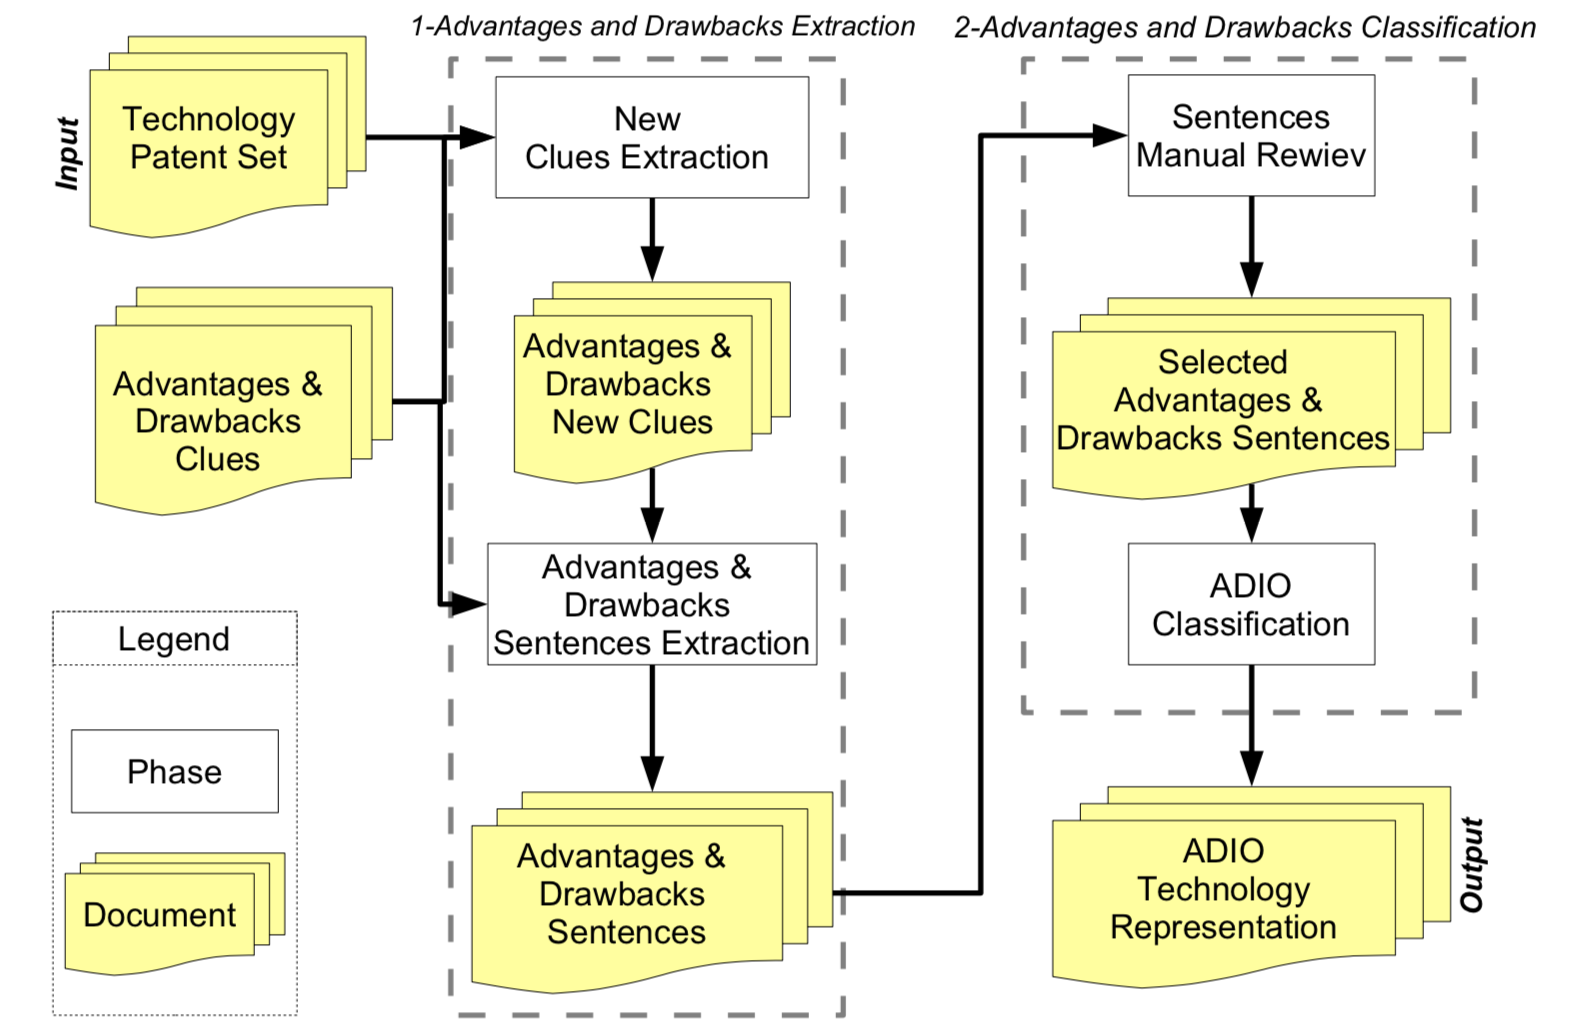
\includegraphics[width=0.8\linewidth]{_bookdown_files/figures/adioworkflow} 

}

\caption{Work flow diagram followed to extract the ADIO technology repres- entation from a patent set.}\label{fig:adioworkflow}
\end{figure}

\subsection{Advantages and drawbacks
extraction}\label{advantages-and-drawbacks-extraction}

The process of advantages and drawbacks extraction is the first of the
two-macro processes used in our system. The first process starts from a
patent set containing patents inherent to a technology and extract
relevant sentences in output. Each sentence describes an advantage or a
drawback of the specific technology. All steps of this process are fully
automatic. The patent set should be very large, in the order of several
hundred (in our case study n \textgreater{} 1000 items). To describe
with a certain degree of precision an advantage or a drawback, patent
applicants have to use sentences of a certain length. Since NER systems
are designed to extract single words or short n- grams, we need to
extract entities that are clues of the whole sentence that describes the
advantage or the drawback. However our interest is not on the clue but
rather on the words that follows the clue: the real advantage or the
real drawback. We refer to these words as target. Considering the ADIO
classification, proposed in the present work, these are words that help
to classify whether the advantage or the drawback have an impact on the
input (influencing efficiency) or the output (influencing effectiveness)
of the system. The few examples above shows how clues are words that
indicates a characteristic of a flow or its modification (positive or
negative); the clue and target together specify the entity and direction
of the modification of the flows that evolve within the system. A
summary of these linguistic concepts and some examples are shown in
figure \ref{fig:audioexamplesent}.

\begin{figure}

{\centering 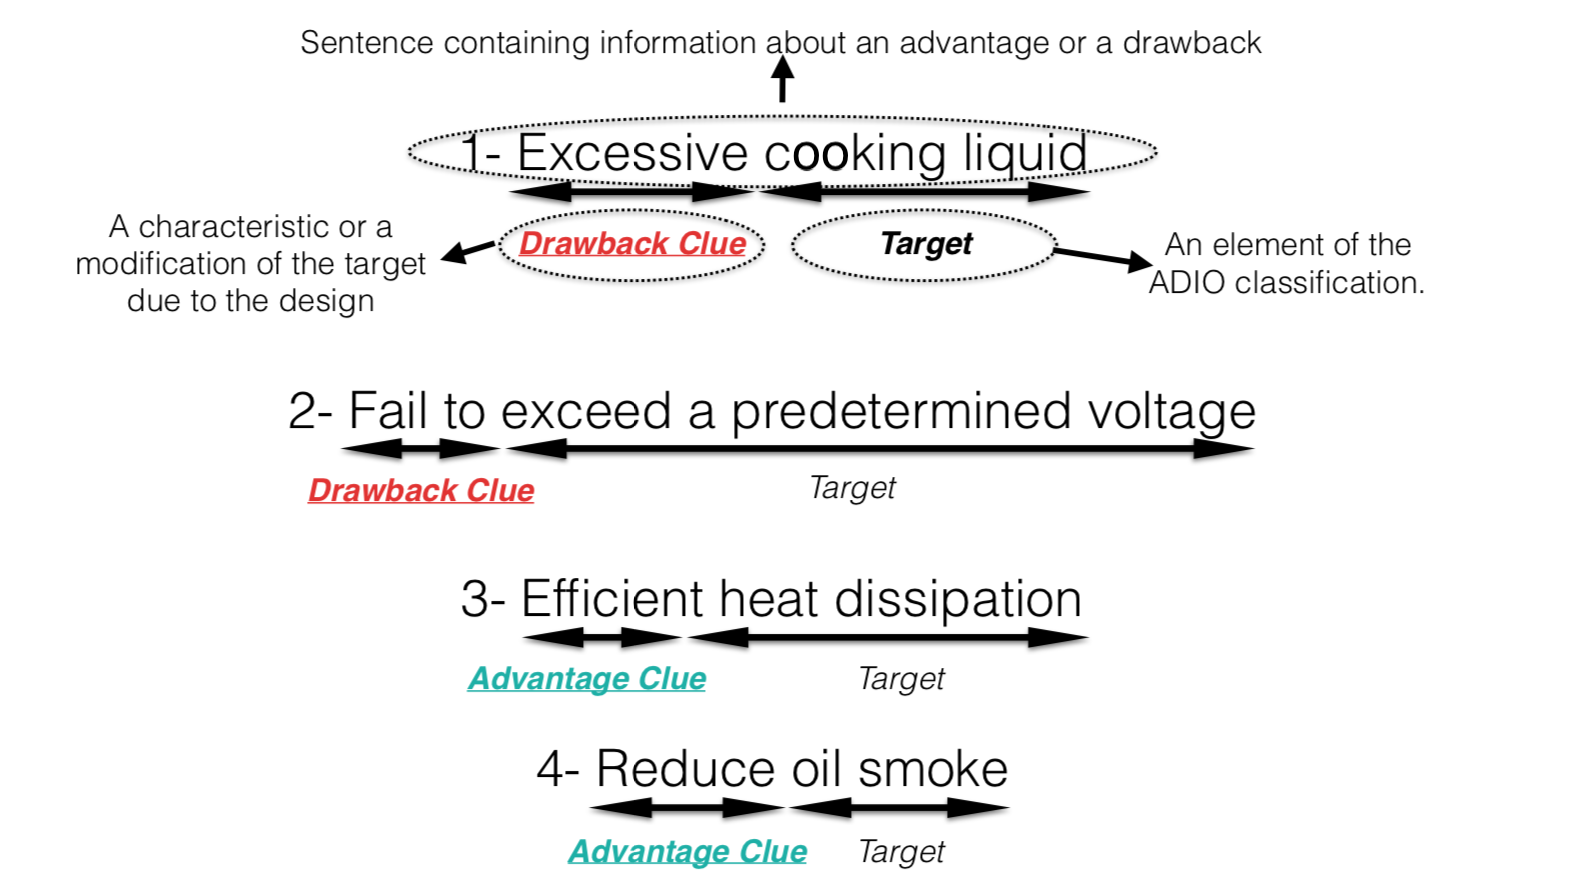
\includegraphics[width=0.8\linewidth]{_bookdown_files/figures/audioexamplesent} 

}

\caption{Examples of advantage or drawback sentences divided in its clue and target.}\label{fig:audioexamplesent}
\end{figure}

As stated above, we introduce a crucial concept, that of a ``clue'' for
the identification of a complex text structure describing advantages or
drawbacks. We describe here the process for collecting clues. The
process is not trivial because the sources are heterogeneous, fragmented
and sparse. For example, we can find lists of failures in repositories
published in the car industry, lists of diseases or infections in
medical treatises, lists of positive and negative words in sentiment
analysis tool-chains. Some of them are very accurate but extremely
short, domain specific and rarely occurring in patents (e.g.~new
diseases), while others are broad but ambiguous thus introducing noise
in the analysis (e.g.~sentiment annotated words). We followed a twofold
approach. The first approach consisted in the manual collection of clues
of advantages and drawbacks directly from patent texts. This process was
performed on 2000 patents in several patent classes. This has led to
collect 3.254 advantage-clues and 5.142 drawback-clues. The second
approach consisted in looking for alternative methods to indicate
advantages or drawbacks clues, finding defined word patterns. The most
relevant are the negations of advantages to obtain drawbacks, and the
negation of drawbacks to obtain advantages. It is worth noting the cases
of suffixes like as -less or -friendly, - free and the like, and
prefixes like as anti-, dis- , de-, un- and the like, that allow a rapid
and systematic expansion of the database. At the end of the process,
advantages numbered 6.568 and the drawbacks numbered 14.809. This is a
fairly large knowledge base for the system, and gave us a reasonable
number of clues to be used in the next step of the process. Example of
clues are shown in section \ref{advdrwresults}. The first approach has
the limitation that lists were extracted from a random but relatively
small sample of patents (n= 2000). Another limitation is that the rules
used in the second approach are not exhaustive, and they can create
non-sense clues, due to the possible combinations of words (e.g. ``anti-
ability'' or ``un-problem''). On the positive side, it is reasonable to
assume that using these approaches it is possible to collect a large set
of clues that are relatively independent from the patent set. In
addition, it is now clear how new clues could be easily extracted when
changing patent sets. In order to obtain a larger and complete
collection of clues it is unsuitable to use the manual extraction on
each domain patent set. For this reason, new clues were iteratively used
to train machine learning algorithms.

\subsubsection*{New Clues Extraction}\label{new-clues-extraction}
\addcontentsline{toc}{subsubsection}{New Clues Extraction}

In this section we briefly describe the system used to automatically
extract new word clues from patent texts. The system is based on the
work discussed in section \ref{advdrwresults}. This process takes in
input a corpus of patent documents regarding a certain technology. After
the tokenization of the corpus, each token (word or n-gram) is
represented by series of features. Then the advantage and drawback clues
are re-projected on the text, generating a training set of words to be
given as an input to a classifier system. The classifier builds a model
able to detect words that have similar behavior (in terms of the
selected features) with respect to the behavior described in the
training set. The model is used to classify the words contained in
patents as potential new advantages or drawbacks word clues. These new
words clues are technology specific clues or generic clues that did not
belong to the starting list of advantages and drawbacks generic word
clues.

\subsubsection*{Advantages and Drawbacks Phrases
extraction}\label{advantages-and-drawbacks-phrases-extraction}
\addcontentsline{toc}{subsubsection}{Advantages and Drawbacks Phrases
extraction}

Once all the new advantages and drawbacks clues are extracted, these are
merged with the ones belonging to the original knowledge base, obtaining
a final list which will be processed by the advantages and drawbacks
sentences extractor. The advantages and drawbacks sentences extraction
is the activity through which the system catches the shortest
informative sentence containing each word clues. To do that the patents
are processed through a phase of part-of-speech tagging (POS tagging).
Starting from the clues, only the POS sequences that match a certain
pattern were extracted. The pattern, expressed using a regex regular
expression is:

\begin{equation*} 
(Clue) + Noun.* Noun.* Noun.*
\end{equation*}

This structure has proven to be able to catch a reasonable number of
words of the target, exhaustively expressing an advantage or a drawback
without catching very long phrases.

\subsection{Advantages and Drawbacks ADIO
classification}\label{advantages-and-drawbacks-adio-classification}

The process of advantages and drawbacks classification is the second of
the two macro processes involved in our system. This process takes in
input the advantages and drawback sentences extracted in the advantages
and drawback extraction process and gives in output the ADIO
representation of the technology.

\subsubsection*{Sentences Selection}\label{sentences-selection}
\addcontentsline{toc}{subsubsection}{Sentences Selection}

As stated above, we suggest a clear classification of advantages and
drawbacks in a 3*2 structure. After the extraction each sentence is
assigned to one of the following classes:

\begin{enumerate}
\def\labelenumi{\arabic{enumi}.}
\tightlist
\item
  more/less wanted output obtained. A wanted output is a desired effect
  of the system.
\item
  more/less unwanted output obtained. An unwanted output is undesired
  effect of the system.
\item
  more/less resources needed.
\end{enumerate}

If a sentence does not belong to one of these classes it is not taken in
to consideration for the next analysis, even if expresses advantages or
the drawbacks of the invention. This classification makes it possible to
represent the technology using the ADIO representation.

\subsubsection*{ADIO Technology
Representation}\label{adio-technology-representation}
\addcontentsline{toc}{subsubsection}{ADIO Technology Representation}

Given the classification described above, we obtain three possible kind
of advantages and three possible kinds of drawbacks. Considering a
wanted or desired output, the achievement or the increase is an
advantage, while the negation or the reduction is a drawback. On the
other side, considering an input to the system or an unwanted output,
negation and reduction constitute an advantage, while achievement and
increase are clearly a drawback. It is important to specify that the
both the input or the output (wanted or unwanted) could involve flows of
matter, energy, or signal.

\section{Results}\label{results-10}

\subsection{Patent set}\label{patent-set}

To test the proposed process, we selected a patent set composed of a
sample of 3,000 patents. The patent sets belongs to the A47J37 IPC
patent class defined as \emph{``Baking; Roasting; Grilling; Frying''}.
We will refer to this patent set as cookers set.

\subsection{Extraction of Advantages and
Drawbacks}\label{extraction-of-advantages-and-drawbacks}

Total extracted advantages numbered 4129, drawbacks numbered 1835. After
manual review of sentences the total number went to 2509 and 1532,
respectively. During the manual review phase each sentence was assigned
to one of the three classes of the taxonomy, considering the target of
the sentence. The system itself decides if a sentence indicates an
advantage or a drawback, considering the clue. The results in terms of
cardinality of the classes of the taxonomy are shown in Table
\ref{tab:adiotableresults}. As we can see from this table, the sentences
review process has led to a balance between the extracted advantages and
drawbacks. It is interesting to see how the wanted outputs are more
likely expressed as advantages (1786 sentences are advantageous wanted
output while 660 are drawbacks); the situation is reversed for the
unwanted output (431 sentences or that advantages and 682 for the
drawbacks).

\begin{longtable}[]{@{}lrr@{}}
\caption{\label{tab:adiotableresults} Examples of clues of advantages and
drawbacks extracted manually from patents.}\tabularnewline
\toprule
Class & Number of Advantages Sentences & Number of Drawback
Sentences\tabularnewline
\midrule
\endfirsthead
\toprule
Class & Number of Advantages Sentences & Number of Drawback
Sentences\tabularnewline
\midrule
\endhead
Input & 292 & 190\tabularnewline
Wanted Output & 1786 & 660\tabularnewline
Unwanted Output & 431 & 682\tabularnewline
TOT & 2509 & 1532\tabularnewline
\bottomrule
\end{longtable}

\subsection{A-D-I-O Representation}\label{a-d-i-o-representation}

The two ADIO schemes for the advantages and drawbacks of cookers are
shown respectively in Figure \ref{fig:adiorapresentationout}. The
sentences shown in this figure are a sample of all of the 2662 extracted
sentences. Furthermore these sentences are taken as-is from patents,
misprints and errors included.

\begin{figure}

{\centering 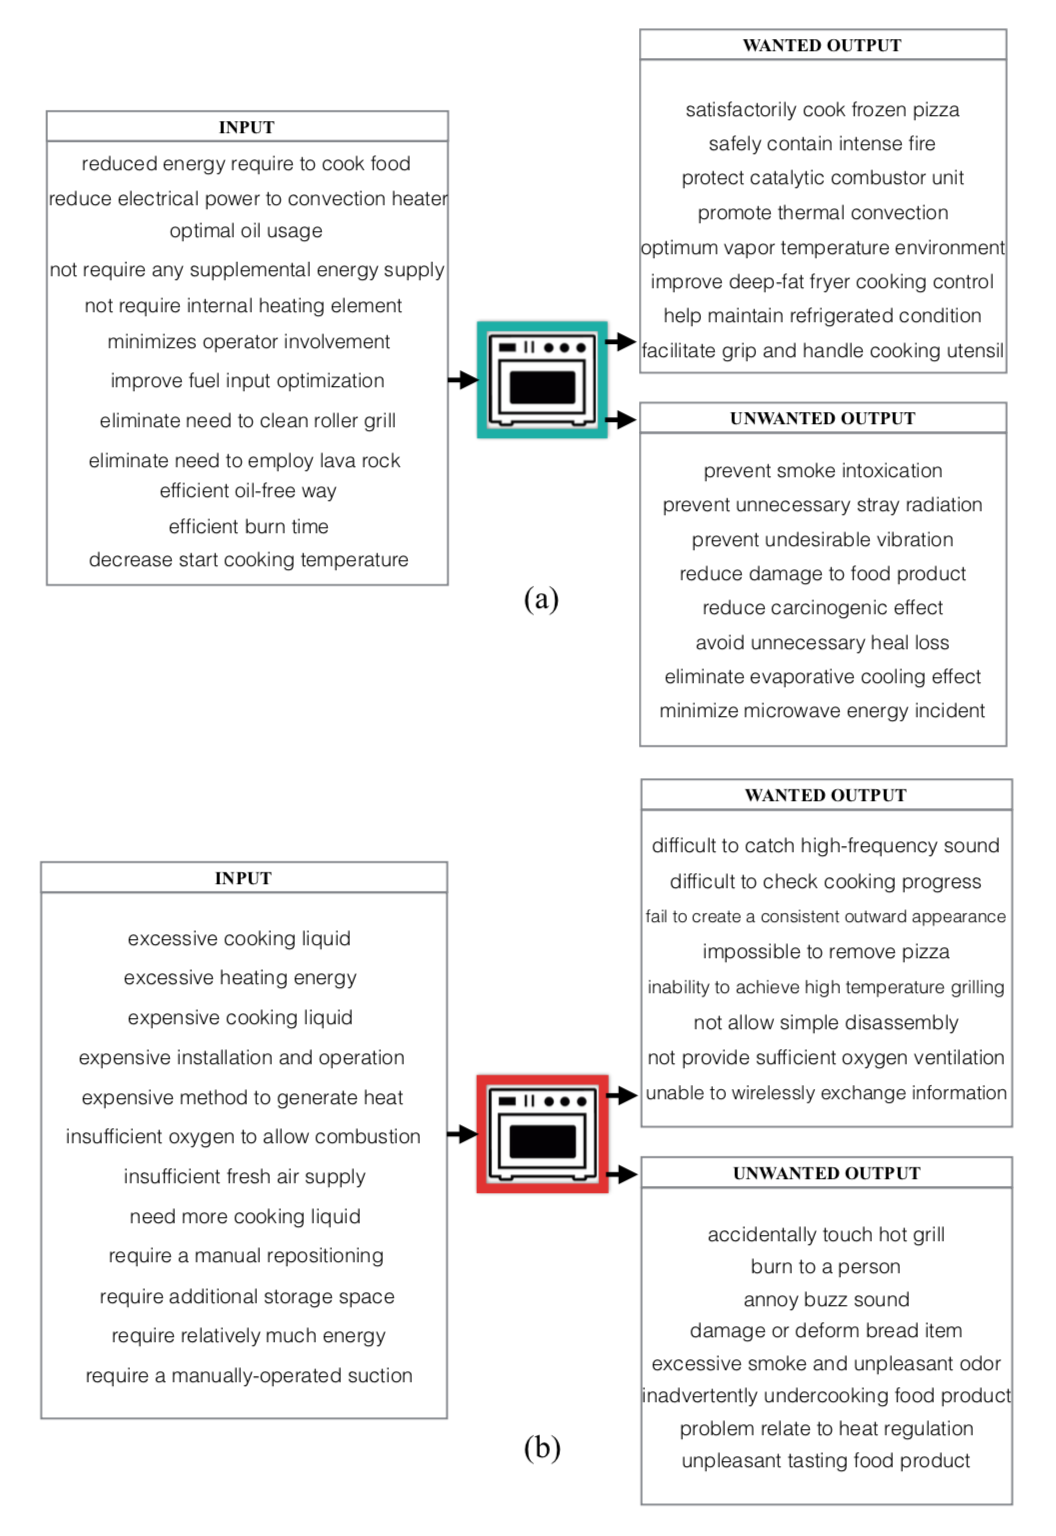
\includegraphics[width=0.8\linewidth]{_bookdown_files/figures/adiorapresentationout} 

}

\caption{Examples of advantage or drawback sentences divided in its clue and target.}\label{fig:adiorapresentationout}
\end{figure}

Both the results are promising for future applications in the design
fields. In particular Figure \ref{fig:adiorapresentationout} (a) allows
designers to focus on the positive side of the effects provided by the
product and to better meet the explicit and implicit user needs.
Similarly, Figure \ref{fig:adiorapresentationout} (b) helps designers to
redesign of the product in a proactive way, to keep attention to the
critical issues identified by the drawbacks and to conceive possible
corrective actions to solve such drawbacks.

\section{Discussion}\label{discussion}

This chapter has proposed a method to extract and summarize sentences
that describe advantages and drawbacks of technologies from patents.
Advantages and drawbacks are considered as phenomena that influence the
efficiency or the effectiveness of products by modifying their inputs or
their outputs. Advantages and drawbacks information are useful for
designers who want to design new products or to redesign old ones so to
meet user needs in novel and better ways. The proposed approach allows
patent readers to analyze a massive quantity of patents and to reduce
the time needed for research and analysis.

\chapter{Enriched dictionaries for
Innovation}\label{enriched-dictionaries-for-innovation}

The demand for intelligence and foresight of technologies is increasing
due to the need of companies and governments to make sense of the
rapidly changing technology landscape and to make better decisions. In
particular, emerging technologies exhibit not only rapid growth, but
also strong conditions of technology and market uncertainty, so that
traditional techniques of technology intelligence are challenged
\citep{rotolo2015emerging}.

Technology intelligence makes large use of a statistical procedure
called clustering. This multivariate technique is commonly used to place
entities into relatively homogeneous groups, maximizing the difference
with other groups, when entities are not subject to an existing
classification. In technology intelligence this is the most interesting
situation: if technologies were already fully classified, then they
would already be established or mature.

It is important to remark that clustering, in one way or another, is
almost a necessity in technology intelligence. The amount of data
available on technologies, even on the last generation of technologies,
is so large that a preliminary effort of clustering and profiling is
generally considered a preliminary step for the analysis.

In technology intelligence the formation of clusters is generally based
on words extracted from relevant documents (scientific publications,
patents, technical standards). There are two main approaches to the
extraction of words from documents: extracting from the metadata
associated to the document, or extracting from the full text of the
document. Examples of metadata are authors, affiliations, inventors,
assignees, keywords, titles. This approach has generated a large
literature that uses metadata in order to extract usable knowledge.
Within this literature, a notable stream of studies has extracted usable
knowledge from documents by clustering the metadata in order to obtain
meaningful structures. This method is associated to the use of keywords,
as we will see below.

More recently, a different approach has been introduced, based on the
processing of the full text of documents. Following the remarkable
advancements in computational linguistics, it has become possible to
process the entire text of publications, patents, or technical standards
to a large scale. Here the clustering exercise does not take place on
metadata, but on words, or their combinations, included in the text of
documents. The topic modeling is the most used approach. Topic modeling
is a tool to extract structures of text from corpora without the help of
external sources of knowledge \citep{blei2003latent}. Once the words
have been extracted from metadata or the full text, a clustering
strategy must be designed based on an appropriate definition of
similarity.

We then suggest the exploration of a novel approach, one that combines
domain knowledge with powerful data science techniques, called
\emph{enriched dictionaries}. These are large and highly structured
collections of words, associated to formal definitions and internal
linkages, that are produced on the basis of domain knowledge of various
kinds. In some cases they are publicly available, in other cases they
are the result of dedicated and idiosyncratic research efforts. These
dictionaries can be used in order to ``filter'' the semantic content of
the full text of documents according to pre-defined structures,
generated within the domain knowledge and validated at the state of the
art. They can be used, therefore, within the so called supervised text
mining approach. This section has two objectives: introducing the
methodology of enriched dictionaries, and showing that it allows the
joint use of several, and complementary, perspectives: one based on the
abstract engineering principles of technologies (functional view),
another on the advantages delivered by the technology (advantage view).
These dimensions are kept separate in the literature and clustering
exercises do not combine them. We show the power of clustering
technologies using these views in a combined way.

\section{An overview of dictionaries for technology
intelligence}\label{an-overview-of-dictionaries-for-technology-intelligence}

\subsection{Publicly available
dictionaries}\label{publicly-available-dictionaries}

One of the advantages of the dictionary approach is the possibility to
utilize publicly available dictionaries, that is, available online with
unrestricted, free access. We made systematic use of Wordnet, a large
dictionary in English language made available and curated by Princeton
University. Wordnet is a standard reference in computational
linguistics.

Upon the basic Wordnet dictionary, several specialized or dedicated
dictionaries have then been developed, which are also available with
unrestricted, free access. We made use of the following dictionaries.

\begin{itemize}
\item
  Artifacts: a collection of terms referring to objects, inventions and
  tools. The dictionary is one of the Name categories available in the
  Wordnet-based categorization dictionary from Provalis, free to
  download \footnote{\url{https://provalisresearch.com/products/content-analysis-software/wordstat-dictionary/wordnet-based-categorization-dictionary}}.
  Artifacts were chosen to explore texts in order to find structural
  indications for the components of an invention.
\item
  Acts: a collection of terms referring to generic actions. This is
  another Name category from the Wordnet dictionary. Acts were selected
  in order to find verbal expressions referable to functions carried out
  by the objects described therein.
\end{itemize}

\subsection{Research-based
dictionaries}\label{research-based-dictionaries}

The dictionary methodology offers the flexibility to build up dedicated
or specialized dictionaries, that represent the state of the art of a
given knowledge domain. We make use of two dedicated dictionaries
recently developed by the authors in an academic research context.
Needless to say, in these cases the authors must give the readers or
users of the dictionary full proof of the completeness of the
dictionary, or the compliance with formal criteria for the definition of
a dictionary. These proofs have been offered in a number of papers cited
below.

\begin{longtable}[]{@{}lrl@{}}
\caption{\label{tab:dictex1} Sources and main characteristics of
dictionaries.}\tabularnewline
\toprule
\begin{minipage}[b]{0.17\columnwidth}\raggedright\strut
Dictionary\strut
\end{minipage} & \begin{minipage}[b]{0.12\columnwidth}\raggedleft\strut
Numberof entries\strut
\end{minipage} & \begin{minipage}[b]{0.62\columnwidth}\raggedright\strut
Examples of chunks\strut
\end{minipage}\tabularnewline
\midrule
\endfirsthead
\toprule
\begin{minipage}[b]{0.17\columnwidth}\raggedright\strut
Dictionary\strut
\end{minipage} & \begin{minipage}[b]{0.12\columnwidth}\raggedleft\strut
Numberof entries\strut
\end{minipage} & \begin{minipage}[b]{0.62\columnwidth}\raggedright\strut
Examples of chunks\strut
\end{minipage}\tabularnewline
\midrule
\endhead
\begin{minipage}[t]{0.17\columnwidth}\raggedright\strut
Artifacts\strut
\end{minipage} & \begin{minipage}[t]{0.12\columnwidth}\raggedleft\strut
12374\strut
\end{minipage} & \begin{minipage}[t]{0.62\columnwidth}\raggedright\strut
Acetanilid, Actuator, Aerogenerator, Agglomerator\strut
\end{minipage}\tabularnewline
\begin{minipage}[t]{0.17\columnwidth}\raggedright\strut
Acts\strut
\end{minipage} & \begin{minipage}[t]{0.12\columnwidth}\raggedleft\strut
5527\strut
\end{minipage} & \begin{minipage}[t]{0.62\columnwidth}\raggedright\strut
Abduction, Abidance, Accenting, Acquiring\strut
\end{minipage}\tabularnewline
\begin{minipage}[t]{0.17\columnwidth}\raggedright\strut
Functional Verbs\strut
\end{minipage} & \begin{minipage}[t]{0.12\columnwidth}\raggedleft\strut
11256\strut
\end{minipage} & \begin{minipage}[t]{0.62\columnwidth}\raggedright\strut
Abrade, Absorb, Abut, Accelerate\strut
\end{minipage}\tabularnewline
\begin{minipage}[t]{0.17\columnwidth}\raggedright\strut
ADV/DIS\strut
\end{minipage} & \begin{minipage}[t]{0.12\columnwidth}\raggedleft\strut
29902\strut
\end{minipage} & \begin{minipage}[t]{0.62\columnwidth}\raggedright\strut
Ability, Accelerate, Acceptance, Accessibility, Accident, Accidents,
Aggravated, Aggravation\strut
\end{minipage}\tabularnewline
\bottomrule
\end{longtable}

\begin{itemize}
\item
  Functional verbs: list of verbal expressions describing functions, or
  actions performed by artifacts on given objects
  \citep{fantoni2013automatic, apreda2016functional}.
\item
  Advantages and Disadvantages: list of terms referring to measurable
  benefits or drawbacks related to an object, chosen for their capacity
  to represent applications of an invention (see section
  \ref{advdrwresults}).
\end{itemize}

Table \ref{tab:dictex1} offers an overview of the dictionaries used for
this analysis, with a few examples of terms.

\section{The value added of enriched
dictionaries}\label{the-value-added-of-enriched-dictionaries}

In order to illustrate the original contribution of the enriched
dictionary approach, it is useful to refer to similar approaches,
recently introduced in the literature. The starting point of this
literature is similar to the one advocated in this paper, i.e.~the need
to supervise the full text mining with the help of list of words that
reflect domain knowledge.

A natural candidate here is the list of words that describe technical
functions, or the abstract characterization of the working principles of
technologies
\citep{cascini2004natural, dewulf2006directed, cascini2007computer, cascini2008measuring}.
The pioneering approach in this field is TRIZ, the patent-based
methodology that has identified a number of abstract inventive
principles \citep{petrov2002laws}, whose application to patent texts has
permitted the detection of evolutionary trends in specific technologies
\citep{verhaegen2009relating, wang2010identifying, yoon2011automated, park2013identification}.
A variant of this approach combines the functional approach with lists
of product attributes or properties
\citep{yoon2012detecting, yoon2011invention, kim2010cause}. More
recently, a similar approach has been introduced, suggesting that
subject-action-object (SAO) linguistic patterns can be derived
automatically from the full text of patents
\citep{yoon2011identifying, choi2012sao, park2011identifying}. A SAO
textual sequence is considered an indication of the engineering
principle that describes an action that is changing an object. Choi et
al \citep{choi2012sao} reviews the state of the art of function-based
technology databases (in particular, TRIZ and Creax) but suggest that
SAO structures are more versatile and flexible in order to apply Natural
Language Processing techniques.

Within this line of investigation the notion of technology tree (Tech
Tree) has been introduced \citep{choi2012sao}. It combines within a
single representation taxonomies of products, technologies, and abstract
functions. Similarity matrices are built along these dimensions and
aggregated.

While these two approaches have generated a large and interesting
literature, their main limitation is the lack of transparency. The
queries obtained from the TRIZ inventive principles have not been
published and there is no demonstration of their reliability
(i.e.~replicability under controlled conditions) with respect to all
semantic variations of words. Similarly, the SAO queries, although
intuitively clear, leave the readers and users with the problem of
establishing the semantic content in the engineering sense, given that
the notion of ``action'' may cover, in fact, many different meanings.

\section{Methodology}\label{methodology-10}

The cited studies have suggested that a mixed approach to the clustering
problem could be the best solution to achieve good results. In
particular there is a need for placing more domain knowledge into the
analysis, while keeping the enormous advantages of text mining and
automatic knowledge representation techniques.

This is the starting point of the dictionary approach we propose. It
suggests that the full text of technical documents is searched by using
a structured list of words, generated from a substantive body of domain
knowledge, formally defined, and organized in a hierarchical way.

A dictionary, in substance, is a collection of terms pertaining to a
precise context and then selected following a logical pattern. The
content of a dictionary may sensibly vary from case to case, comprising
terms related to a precise technology, a technical field, a social
group, or more generic parts-of-speech such as particular kinds of
actions or nouns, and so on.

The main difference between a dictionary and a mere collection of
keywords is in their respective scope, which is, for a dictionary, wider
and far more complete, including all the synonyms, hypernyms and
hyponyms of a term. By definition, a dictionary must include all the
definitions and terms referring to the chosen context. The completeness
has an important consequence for text mining applications. When a
dictionary is used as a tool to filter the content in a collection of
texts, the query is formed not only by principal words, but also by
secondary words, such as synonyms. These secondary words would be lost
if the analysis were based on words and keywords. Therefore dictionaries
contribute to overcoming the biases introduced in the analysis by the
subjective choice of keywords by experts.

To start with, the dictionary method was combined with topic modelling
techniques in order to overcome one of the main limitations of topic
modeling, that is, the extraction of irrelevant topics.

The starting assumption is the possibility of representing a document
using the main topics cited in it. A topic is, basically, a collection
of terms that delineate and describe an argument. Topics may be
identified by using unsupervised or supervised methods. The unsupervised
application of the method will have the result of giving generic topics,
often irrelevant in specialized analysis. This outcome can be mitigated,
but not eliminated, by the application of ranking techniques, such as
Term Frequency-Inverse Document Frequency (TF-IDF), that allow the
identification of coherent topics. Alternatively, analysts may refer to
supervised methods, which are however resource-consuming in their design
and implementation. The dictionary approach offers an excellent solution
to the trade-off between relevance and precision of the search, which
plays in favor of supervised methods, and the parsimony of the analysis,
which on the contrary militates for the adoption of unsupervised
methods.

In addition, if topics are clearly delineated, it becomes possible to
identify similarities between documents that refer to technologies with
a transversal, or cross-domain, potential for application. Dictionaries
can be used for different purposes and help to identify latent
structures from a variety of perspectives. We advocate the use of
several dictionaries in parallel, on the same collection of texts, as a
way to examine technologies with a variety of perspectives. Figure
\ref{fig:dictwf} illustrates the main steps of the methodology.

\begin{figure}

{\centering 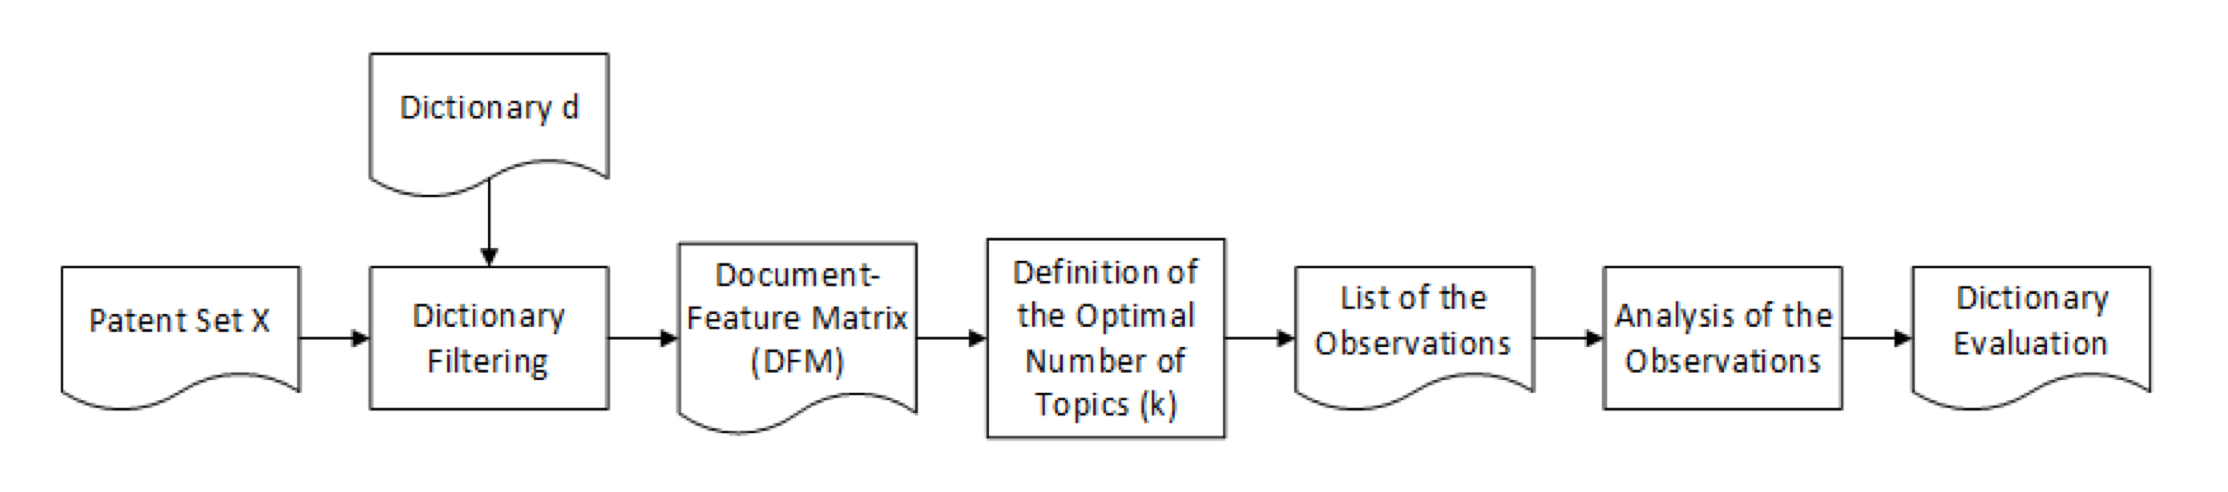
\includegraphics[width=0.8\linewidth]{_bookdown_files/figures/dictwf} 

}

\caption{Steps of the dictionary approach to the text mining of patents.}\label{fig:dictwf}
\end{figure}

The basic idea of the process is that a document can be represented by
the set of terms, numbers, graphic symbols and punctuation that compose
meaningful sentences. The ``technical'' objects belonging to this set
are named Features. Starting from selected patent sets, a
Document-Feature Matrix is created using different dictionaries as
filters to select only the desired features; the obtained matrices are
then used as the starting point to perform a topics number evaluation
algorithm, based on the connections between documents with same or
similar features. Topics are formally clusters of features, coupled
because of their pertinence to the same concept; measuring the
percentage of cohesion of a document to each topic recognized is, then,
a method to collect information about the contents of the document
itself.

\subsubsection*{Creation of the Document-Feature
Matrix}\label{creation-of-the-document-feature-matrix}
\addcontentsline{toc}{subsubsection}{Creation of the Document-Feature
Matrix}

A patent can be represented by a vector exhibiting the number of
occurrences, if a given feature is included, and 0 otherwise. Since
these features are ordered within dictionaries, all patents in a patent
set can be represented with similar vectors. A collection of texts can
be therefore represented as a matrix called Document-Feature. A Document
Feature Matrix (DFM) is a algebraic matrix with N rows, corresponding to
individual documents in the corpus, and M columns representing the
features. With this formalization it is possible to measure the
occurrences of features in every document contained in the corpus. It is
a powerful tool to get a fast quantitative information about a document
set, counting the features originated in the dictionaries, with the
opportunity of selecting (or removing) some of them.

Each patent in the patent set is filtered using one of the four
dictionaries at a time. The resulting list of words was processed in
order to eliminate the generic words, or those words that, being
diffused across most documents, do not have specific semantic content.
This is done by using the stopwords labelled SMART in the text mining
literature, in combination with a list of stopwords extracted from the
text of patents and including some generic words in the legal language
of patents (or ``Patentese''), such as claim, invention, right, tool
etc.

Due to the large number of entries in dictionaries and the exploratory
nature of this work, we restricted the number of features considered for
each of the DFMs to 500. The selection was made automatically, by
selecting the top 500 terms in terms of share of documents in which they
appear. In some cases the selected patent text delivered no matching
with the selected features. In this case the patents were eliminated.
Thus the final DFM only includes documents with positive entries from
the lists of features extracted from the analysis. It must be noted that
DFMs are sparse matrices: sparsity is a mathematical parameter, varying
from 0 to 1, that indicates how much systems are loosely coupled. In
particular, it is a measure of the Z zero-valued elements in a matrix
divided by the N x M total number of elements. Thus, a sparse matrix is
a matrix in which large part of elements in cells are zeroes. Sparsity
it is a good measure of how documents in a corpus differ from each other
with respect to their Features.

Documents are iteratively examined in pairs: if two documents share a
feature they are considered similar. Various metrics of similarity can
be defined and computed. After a measure of similarity is defined,
various clustering techniques can be applied as well. In this
application we use the cosine similarity, which is largely adopted in
the field. Cosine similarity is a measure of similarity between two
non-zero vectors, that computes the cosine of the angle between them in
an inner product space. Each document in the Document-feature Matrix is
characterized by a vector where the value of each dimension corresponds
to the number of times the feature appears in the document. Two
documents, then, are similar if their cosine similarity is near to 1.

Given two n-dimensional vectors of attributes, x and y, their cosine
similarity is calculated by the dot product of them, normalized by the
product of the vector lengths. Results of the similarity measures are
stored in a N x N matrix, in which documents are both upon rows and
columns. It is a squared matrix with ones on its diagonal, indicating
identities between patents and themselves, and the upper (or lower, for
it is the same) half filled with similarity values for all the document
couples. The most intuitive method to analyze which patents are more
similar is to visualize them in a graph. To do so, it was used the
igraph package , which contains a list of commands for creating and
analyzing graphs. We can use our similarity matrices as a base to build
the corresponding graphs, using them as they were adjacency matrices.

\subsubsection*{Adjacency Matrix}\label{adjacency-matrix}
\addcontentsline{toc}{subsubsection}{Adjacency Matrix}

An Adjacency Matrix is a square matrix that represents a finite graph.
In this case, the similarity matrix has in position (i,j) the inverse of
the distance between vertices vi and vj . This gives to the graph not
only information about whether two vertices are connected, but also a
measure of their connection. It was chosen to set a threshold t = 0.8
for similarities in order to avoid representation of loose relations
between vertices. To better visualize results, graphs were migrated from
R to Gephi, a visualization software that simplifies this kind of
operations. Gephi makes possible to assign colors to nodes as an
intuitive way to label them; in our graphs four different colors were
used to partition patents in their class, then Force Atlas layout
algorithm was performed to see how well the graphs were clustered.

\subsubsection*{Optimal Number of
Topics}\label{optimal-number-of-topics}
\addcontentsline{toc}{subsubsection}{Optimal Number of Topics}

Once created, a DFM can be interpreted as a graph showing similarity
links between documents. In this context, in fact, similarity can be
defined in terms of the percentage of total features that are shared
between documents. Features can also be grouped in topics. In turn,
similarity between documents can be defined in terms of the percentage
of topics shared between documents. Finally, documents that refer to the
same topic, hence are similar among them, can be grouped in cluster.
Within a cluster it is possible to define a metrics of cohesiveness: the
larger the number of topics shared by documents, the larger the
cohesiveness of the cluster they belong to.

The optimal number of topics is not defined once and for all, but it
depends in subtle ways from the characteristics of the documents in the
set and the list of features. Thus the optimal number is the result of
an experimental approach. The R package ldatuning calculates several
metrics and then delivers an estimate on the optimal number of topics
for Latent Dirichlet Allocation (LDA) models. In our application, we
chose the CAOJUAN metric to evaluate the number of topics. The decision
to use just one metric was made due to computational reasons; we
selected the model proposed by Cao Juan, since he demonstrated that LDA
models perform in an optimal way when the average cosine distance of
topics reaches the minimum. Starting from the assumption that less
correlated topics are more independent, the author defined average
dispersion as a metric to measure the topic structure, using cosine
distance. A smaller average dispersion denotes a more stable topic
structure, that is, a topic model which is defined in a better way.

\section{Results}\label{results-11}

We now turn to the analysis of the topics resulting from the filtering
procedure based on dictionaries, the construction of the DFM, the
measurement of cosine similarity. We will use four measures to highlight
the content of the patent sets:

\begin{itemize}
\tightlist
\item
  Average cosine distance of topics
\item
  Average number of topics
\item
  Average sparsity of DFM
\end{itemize}

The dictionaries were divided in two macro-classes, due to their nature:
Non-Technical Dictionaries (Acts and Artifacts) versus Technical
Dictionaries (Functional Verbs and Advantages \& Disadvantages). The
Blacklist set, filtered with canonical and ``Patentese'' stopwords, will
be useful for a more complete understanding of the findings.

In order to test the dictionary approach to clustering, we trained the
algorithm on a standard patent set, formed by patents belonging to four
IPC classes whose technologies are largely known. Table
\ref{tab:dicpatents} illustrates the International Patent Classification
(IPC) classes included in the analysis (a random sample of 2.000 patents
each).

\begin{table}

\caption{\label{tab:dicpatents}Patent sets under examination.}
\centering
\begin{tabular}[t]{>{}l>{\em\raggedright\arraybackslash}p{30em}}
\toprule
IPC Class & IPC Definition\\
\midrule
A47J37 & KITCHEN EQUIPMENT; BAKING DEVICES; ROASTING DEVICES; GRILLING DEVICES; FRYING DEVICES\\
A61C15 & DENTISTRY; APPARATUS OR METHODS FOR ORAL OR DENTAL HYGIENE\\
A61G13 & TRANSPORT, PERSONAL CONVEYANCES, OR ACCOMMODATION SPECIALLY ADAPTED FOR PATIENTS OR DISABLED PERSONS; OPERATING TABLES OR CHAIRS; CHAIRS FOR DENTISTRY; FUNERAL DEVICES\\
A61H & PHYSICAL THERAPY APPARATUS, e.g. DEVICES FOR LOCATING OR STIMULATING REFLEX POINTS IN THE BODY; ARTIFICIAL RESPIRATION; MASSAGE; BATHING DEVICES FOR SPECIAL THERAPEUTIC OR HYGIENIC PURPOSES OR SPECIFIC PARTS OF THE BODY\\
\bottomrule
\end{tabular}
\end{table}

The technologies examined are largely mature. As it is shown in Figure
\ref{fig:dicttrendsipc}, in some of them the patenting activity started
as early as XIX century. The maturity of these technologies is a good
starting condition for the training set: similarities and
dissimilarities of the patents should be clearly visible.

By placing them together in the same patent set we deliberately include
very different technologies. We ask the algorithm based on dictionaries
to be able to discriminate technologies in a patent set which is, by
construction, highly heterogeneous.

\begin{figure}

{\centering 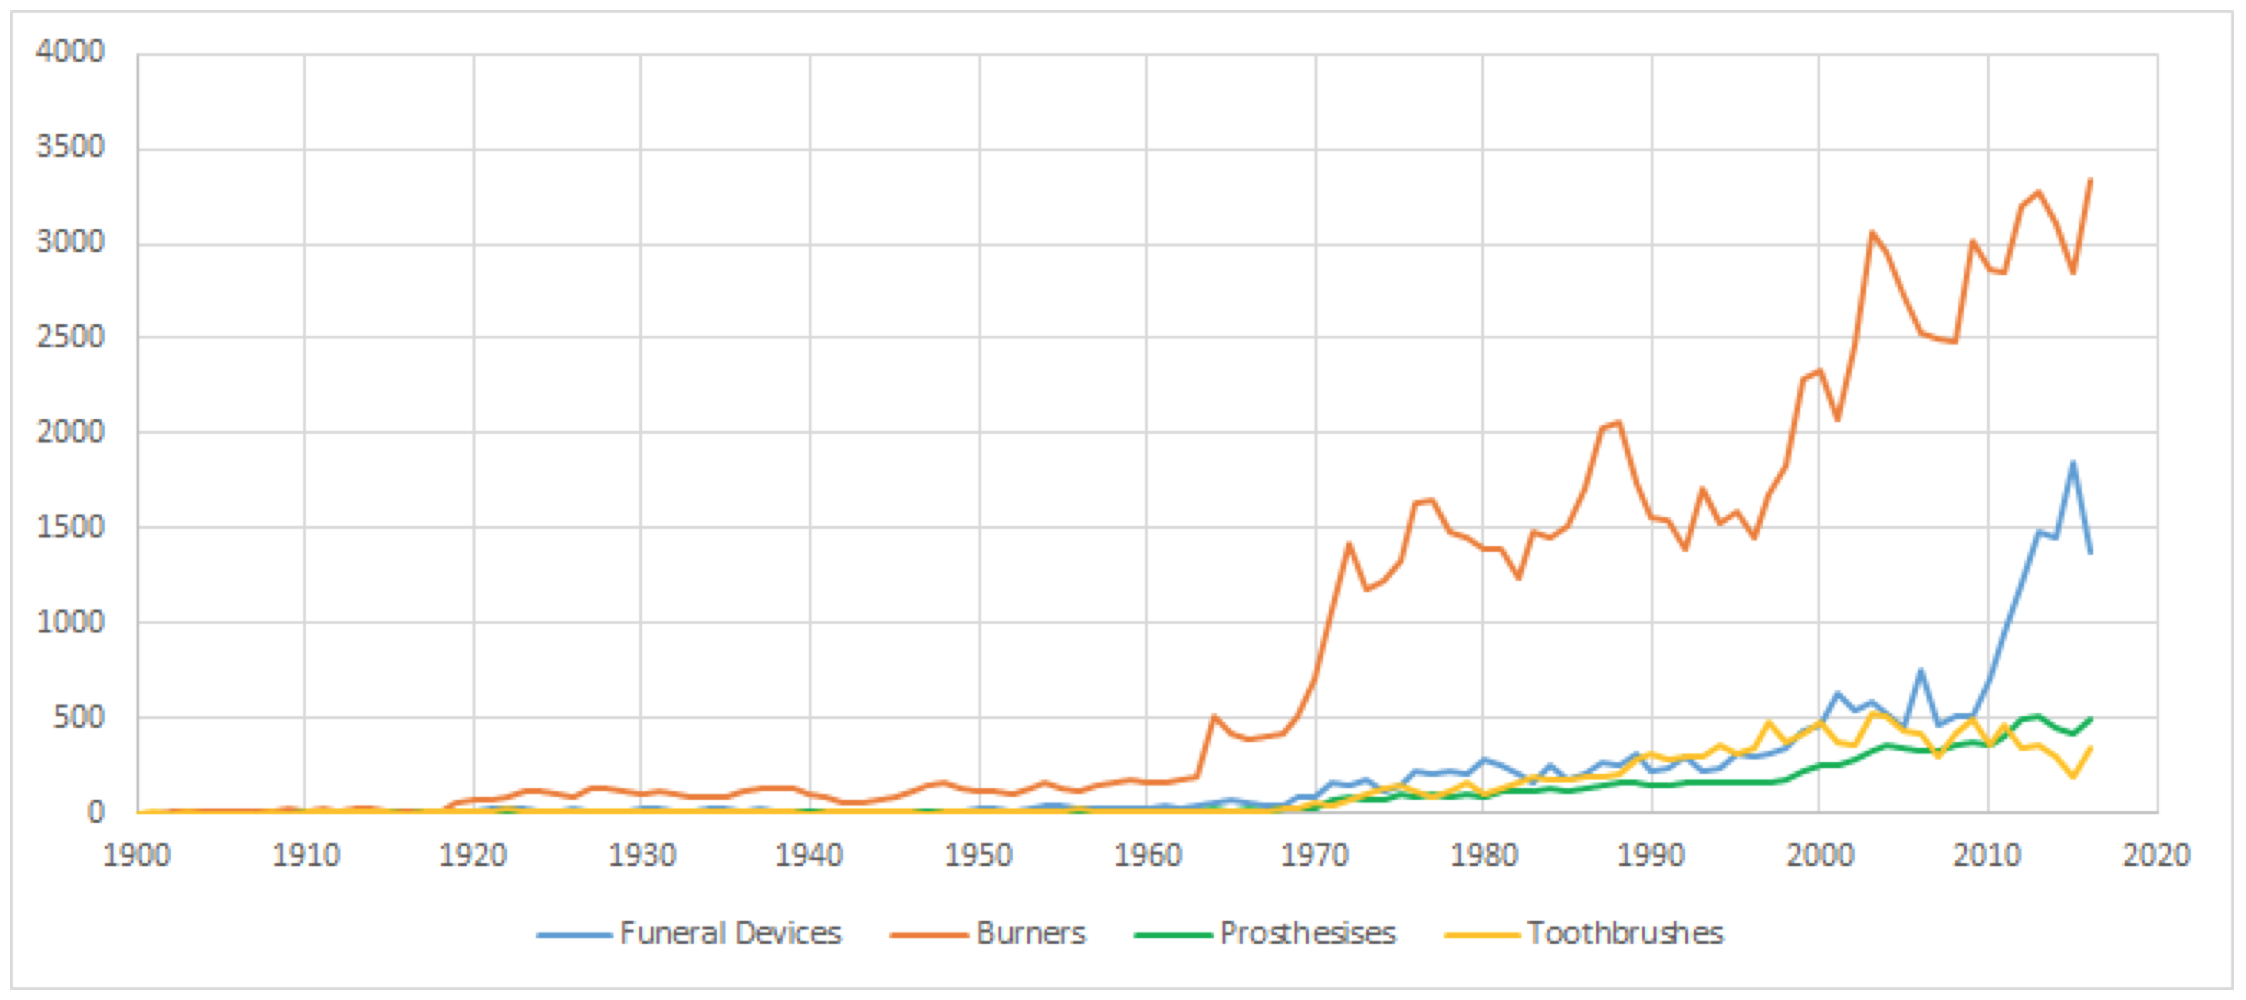
\includegraphics[width=0.8\linewidth]{_bookdown_files/figures/dicttrendsipc} 

}

\caption{Technological history of the technologies in the selected patent sets.}\label{fig:dicttrendsipc}
\end{figure}

Table \ref{tab:dictmetrix} offers a summary of measures derived from the
application of dictionaries to the four patent sets combined together.

\begin{table}

\caption{\label{tab:dictmetrix}Summary of findings from the application of dictionaries to the combined patent sets.}
\centering
\begin{tabular}[t]{>{\raggedright\arraybackslash}p{5em}>{\raggedleft\arraybackslash}p{10em}>{\raggedleft\arraybackslash}p{10em}>{\raggedleft\arraybackslash}p{10em}}
\toprule
Dictionary & Average cosine distance of topics & Average number of topics & Average sparsity of the DFM\\
\midrule
Artifacts & 0.002 & 16 & 98.3\\
Acts & 0.004 & 11 & 97.9\\
Advantages and Disadvantages & 0.016 & 32 & 94.3\\
Functional Verbs & 0.029 & 37 & 73.8\\
Blacklist & 0.031 & 40 & 63.3\\
\bottomrule
\end{tabular}
\end{table}

Two findings are visible in Table \ref{tab:dictmetrix}. First, there is
large difference in the cohesiveness of the clustering based on
Technical and Non-technical dictionaries. The average cosine distance
calculated with the Artifacts and Acts dictionaries is ten times smaller
than the average cosine distance for Advantages \& disadvantages and the
Functional dictionary. Second, Non-technical dictionaries give origin to
a much smaller number of topics.

Let us examine the differences between dictionaries more in detail. We
start by examining the performance of each dictionary in extracting and
clustering topics.

\subsubsection*{Non-technical
Dictionaries}\label{non-technical-dictionaries}
\addcontentsline{toc}{subsubsection}{Non-technical Dictionaries}

Table \ref{tab:dictactsresults} shows the results of the application of
the Acts dictionary to the four separate patent sets, while Table
\ref{tab:dictartsresults} shows the same for the Artifacts dictionary.

\rowcolors{2}{gray!6}{white}

\begin{table}

\caption{\label{tab:dictactsresults}Findings from the application of the Acts dictionary to selected patent sets.}
\centering
\resizebox{\linewidth}{!}{
\begin{tabular}[t]{lrrrrr}
\hiderowcolors
\toprule
Dataset & Number of topics & Cosine distance of topics & Number of documents & Number of features & Average sparsity of the DFM (\%)\\
\midrule
\showrowcolors
Burners & 2 & 0.001 & 496 & 306 & 97.8\\
Toothbrushes & 6 & 0.002 & 494 & 311 & 97.8\\
Prosthesis & 18 & 0.005 & 491 & 493 & 97.9\\
Funeral Dev. & 16 & 0.007 & 491 & 470 & 98.2\\
Mean & 11 & 0.004 & 493 & 395 & 97.9\\
\bottomrule
\end{tabular}}
\end{table}

\rowcolors{2}{white}{white}

\rowcolors{2}{gray!6}{white}

\begin{table}

\caption{\label{tab:dictartsresults}Findings from the application of the Artifacts dictionary to selected patent sets.}
\centering
\resizebox{\linewidth}{!}{
\begin{tabular}[t]{lrrrrr}
\hiderowcolors
\toprule
Dataset & Number of topics & Cosine distance of topics & Number of documents & Number of features & Average sparsity of the DFM (\%)\\
\midrule
\showrowcolors
Burners & 6 & 0.001 & 495 & 397 & 98.4\\
Toothbrushes & 16 & 0.001 & 469 & 500 & 98.8\\
Prosthesis & 18 & 0.003 & 487 & 500 & 98.0\\
Funeral Dev. & 22 & 0.002 & 485 & 500 & 98.1\\
Mean & 16 & 0.002 & 484 & 474 & 98.3\\
\bottomrule
\end{tabular}}
\end{table}

\rowcolors{2}{white}{white}

These two dictionaries were retrieved from the Wordnet categorization
dictionary, which is a tool for linguistic analysis; thus, the terms
comprised in them are of common use, and their suitability for the
description of patents is not guaranteed. Taken together the
Non-technical dictionaries deliver two main results. First, there is a
difference in the optimal number of topics between simple technologies
(Burners and Toothbrushes) and more complex and articulated technologies
(Prosthesis and Funeral devices). In the case of the Acts dictionary,
the optimal number of topics is 2-6 for the former technologies and
18-16 for the latter. Second, Non-technical dictionaries deliver
clusters with an extremely low cosine distance, that is, with strong
internal cohesiveness. In other words, Non-technical dictionaries
produce an excellent clustering of documents. This suggests that they
can be used to obtain a small number of non-technical topics, that allow
a general identification of the content of documents, but not the
identification of technical similarities and differences.

To provide an example of the potential of the dictionary methodology we
show in Tables \ref{tab:acttopicresults} and \ref{tab:arttopicresults}
the top ten words found in a selection of the topics extracted with the
Non-technical dictionaries in the patent set Prosthesis. We need to test
whether Non-technical dictionaries deliver topics that are satisfactory
with respect to their potential to describe technologies.

\begin{table}

\caption{\label{tab:acttopicresults}Top ten words in selected topics extracted in the patent set Prosthesis with the aid of the Acts dictionary.}
\centering
\begin{tabular}[t]{>{\em\raggedright\arraybackslash}p{10em}l>{\em\raggedright\arraybackslash}p{10em}l}
\toprule
Topic 3: Term & Topic 3: Beta & Topic 7: Term & Topic 7: Beta\\
\midrule
Measuring & 0.322 & Manipulation & 0.160\\
Measurement & 0.217 & Steering & 0.152\\
Detecting & 0.210 & Dialysis & 0.145\\
Performing & 0.033 & Cycling & 0.063\\
Sending & 0.031 & Deactivation & 0.060\\
\addlinespace
Calibration & 0.030 & Dampening & 0.049\\
Supplying & 0.024 & Shearing & 0.047\\
Repositioning & 0.024 & Logging & 0.032\\
Causing & 0.009 & Exercising & 0.029\\
Comparing & 0.009 & Reaching & 0.023\\
\bottomrule
\end{tabular}
\end{table}

\begin{table}

\caption{\label{tab:arttopicresults}Top ten words in selected topics extracted in the patent set Prosthesis with the aid of the Artifacts dictionary.}
\centering
\begin{tabular}[t]{>{\em\raggedright\arraybackslash}p{10em}l>{\em\raggedright\arraybackslash}p{10em}l}
\toprule
Topic 5: Term & Topic 5: Beta & Topic 14: Term & Topic 14: Beta\\
\midrule
Backrest & 0.498 & Electrode & 0.405\\
Eyewash & 0.092 & Catheter & 0.233\\
Armrest & 0.085 & Circuitry & 0.106\\
Gasket & 0.060 & Sensor & 0.026\\
Capacitor & 0.052 & Housing & 0.025\\
\addlinespace
Arms & 0.048 & Converter & 0.025\\
Gurney & 0.045 & Emitter & 0.021\\
Footplate & 0.025 & Cathode & 0.018\\
Eyepiece & 0.019 & Anode & 0.018\\
Headrest & 0.011 & Reflector & 0.011\\
\bottomrule
\end{tabular}
\end{table}

In the case of the Artifacts dictionary, Topic 5 gives us information on
components related to the body part interested by the prosthesis, while
Topic 14 tells us about electrical tools and sensors that are involved
in the invention. Also in this case, the two groups are useful to gather
information about the basic composition of the set, but not enough on
focus to have a satisfactory definition of the technologies.

\subsubsection*{Technical Dictionaries}\label{technical-dictionaries}
\addcontentsline{toc}{subsubsection}{Technical Dictionaries}

Table \ref{tab:dictadvsresults} shows the results of the application of
the Advantages \& Disadvantages dictionary to the four separate patent
sets, while Table \ref{tab:dictfunctsresults} shows the same for the
Functional dictionary. The technical dictionaries applied contain a
large number of features, generating a large DFM. An overall look at
Tables \ref{tab:dictadvsresults} and \ref{tab:dictfunctsresults} shows
several interesting findings. First of all, the technical dictionaries
allow the identification of a much larger number of topics with respect
to non-technical dictionaries: the average number is 32 for the
Advantages \& Disadvantages, and 37 for the Functional dictionary. This
means that technical dictionaries show a higher power of discrimination
of semantic content. This is an important finding for Technology
intelligence, since a larger number of internally coherent topics is an
extremely useful starting point for the interpretation of their content.

\rowcolors{2}{gray!6}{white}

\begin{table}

\caption{\label{tab:dictadvsresults}Findings from the application of the Advantages and Disadvantages dictionary to selected patent sets.}
\centering
\resizebox{\linewidth}{!}{
\begin{tabular}[t]{lrrrrr}
\hiderowcolors
\toprule
Dataset & Number of topics & Cosine distance of topics & Number of documents & Number of features & Average sparsity of the DFM (\%)\\
\midrule
\showrowcolors
Burners & 32 & 0.015 & 500 & 500 & 95.9\\
Toothbrushes & 30 & 0.014 & 500 & 500 & 95.0\\
Prosthesis & 32 & 0.021 & 497 & 500 & 92.3\\
Funeral Dev. & 34 & 0.014 & 495 & 500 & 94.0\\
Mean & 32 & 0.016 & 498 & 500 & 94.3\\
\bottomrule
\end{tabular}}
\end{table}

\rowcolors{2}{white}{white}

\rowcolors{2}{gray!6}{white}

\begin{table}

\caption{\label{tab:dictfunctsresults}Findings from the application of the Functional dictionary to selected patent sets.}
\centering
\resizebox{\linewidth}{!}{
\begin{tabular}[t]{lrrrrr}
\hiderowcolors
\toprule
Dataset & Number of topics & Cosine distance of topics & Number of documents & Number of features & Average sparsity of the DFM (\%)\\
\midrule
\showrowcolors
Burners & 38 & 0.021 & 500 & 500 & 76.6\\
Toothbrushes & 36 & 0.022 & 500 & 500 & 75.5\\
Prosthesis & 34 & 0.032 & 497 & 500 & 70.6\\
Funeral Dev. & 38 & 0.041 & 495 & 500 & 72.4\\
Mean & 37 & 0.029 & 498 & 500 & 73.8\\
\bottomrule
\end{tabular}}
\end{table}

\rowcolors{2}{white}{white}

Second, in the case of the Functional dictionary the Document-Feature
Matrix (DFMs) is less sparse: the average sparsity index is 73,8\%, as
opposed to around 98\% for the non-technical dictionaries and 94,3\% for
the Advantages \& Disadvantages dictionary. Third, the total number of
documents used, i.e.~the documents in which there is at least one
matching between the words and the features of the dictionary, is larger
in the case of technical dictionaries (in particular, it is 498 out of
500 for the Functional dictionary).

Fourth, the cosine distance of topics is approximately ten times larger
in the case of technical dictionaries, meaning that clusters enjoy a
over cohesiveness. These findings point to an important contribution of
technical dictionaries, and in particular of the Functional dictionary,
to Technology intelligence, that is, technology mapping, clustering,
interpretation, and foresight.

The Functional dictionary offers a large number of features that find a
matching with the text of the patents, so that the resulting DFM is less
sparse. The fact that the total number of topics is larger also means
that each of the topics is populated by a smaller number of features.
Each topic, therefore, lends itself to a clear understanding of the
technical content. The differences between topics have also a clear
technical interpretation.

It can be said that technical dictionaries, as opposed to non-technical
dictionaries, allow a fine-grained intelligence of the technical content
of patent sets. This is in itself an important achievement, given that
the topic modelling algorithm has not been previously trained, but is
only filtered by the dictionary. In practice we achieve the precise
results of supervised topic modeling with an effort which is more
similar to that of the unsupervised approach.

In order to give a better understanding of the potential of the
technical dictionary approach, let us examine more in detail in table
\ref{tab:advtopicresults} and \ref{tab:functtopicresults} the top 10
words in some of the topics identified in one of the four patent sets
examined, namely Prosthesis.

\begin{table}

\caption{\label{tab:advtopicresults}Top ten words in selected topics extracted in the patent set Prosthesis with the aid of the Advantages and Disadvantages dictionary.}
\centering
\begin{tabular}[t]{>{\em\raggedright\arraybackslash}p{10em}l>{\em\raggedright\arraybackslash}p{10em}l}
\toprule
Topic 6: Term & Topic 6: Beta & Topic 28: Term & Topic 28: Beta\\
\midrule
Adjustable & 0.564 & Worn & 0.155\\
Accommodate & 0.046 & Comfort & 0.086\\
Ergonomic & 0.032 & Wearing & 0.077\\
Securely & 0.022 & Comfortable & 0.058\\
Adjustability & 0.020 & Injury & 0.043\\
\addlinespace
Ability & 0.017 & Discomfort & 0.031\\
Facilitate & 0.016 & Increase & 0.029\\
Stabilizing & 0.011 & Reduce & 0.026\\
Comfort & 0.010 & Uncomfortable & 0.025\\
Stability & 0.010 & Tear & 0.024\\
\bottomrule
\end{tabular}
\end{table}

\begin{table}

\caption{\label{tab:functtopicresults}Top ten words in selected topics extracted in the patent set Prosthesis with the aid of the Functional dictionary.}
\centering
\begin{tabular}[t]{>{\em\raggedright\arraybackslash}p{10em}l>{\em\raggedright\arraybackslash}p{10em}l}
\toprule
Topic 15: Term & Topic 15: Beta & Topic 20: Term & Topic 20 :Beta\\
\midrule
Distance & 0.054 & Arm & 0.238\\
Coupling & 0.053 & Exercise & 0.082\\
Position & 0.052 & Arms & 0.060\\
Neck & 0.043 & Stretching & 0.042\\
Line & 0.041 & Left & 0.025\\
\addlinespace
Parallel & 0.030 & View & 0.024\\
View & 0.021 & Orientation & 0.023\\
Form & 0.019 & Stretch & 0.021\\
Orientation & 0.016 & Angle & 0.019\\
Contact & 0.013 & Tension & 0.017\\
\bottomrule
\end{tabular}
\end{table}

In Table \ref{tab:advtopicresults} Topic 6 calls the attention to
features of the prosthesis such as adjustability, facilitation and
stability, that is, on ergonomic features. Topic 28 emphasizes comfort
(as an advantage made possible by the invention) or discomfort (as a
disadvantage addressed by the invention). The content of these topics,
thanks to the power of the technical dictionary, is crystal clear.

In Table \ref{tab:functtopicresults} we see, in topic 15, the
positioning of prosthesis on the neck of patients, and in topic 20, the
orientation of arms with the support of prosthesis. Both these topics
deal with the issue of placing the prosthesis around or over various
parts of the human body. It is important to underline that, once
generated, topics can also be combined together in further steps of the
analysis.

\subsubsection*{Blacklist}\label{blacklist}
\addcontentsline{toc}{subsubsection}{Blacklist}

Finally, the information power of technical dictionaries can be
appreciated by comparing the results with those that would be obtained
by filtering the texts with semantically poor words, such as generic
words (stopwords) and ``patentese'' generic words. As stated above, the
combination between generic and patentese stopwords is labelled
Blacklist.

\rowcolors{2}{gray!6}{white}

\begin{table}

\caption{\label{tab:dictblacklist}Top ten words in selected topics extracted in the four patent sets with the aid of the Blacklist.}
\centering
\resizebox{\linewidth}{!}{
\begin{tabular}[t]{lrrrrr}
\hiderowcolors
\toprule
Dataset & Number of topics & Cosine Distance of Topics & Number of documents & Number of features & Average sparsity of the DFM (\%)\\
\midrule
\showrowcolors
Burners & 40 & 0.016 & 500 & 500 & 66.5\\
Toothbrushes & 40 & 0.025 & 500 & 500 & 65.7\\
Prosthesis & 40 & 0.040 & 500 & 500 & 59.2\\
Funeral Dev. & 40 & 0.042 & 500 & 500 & 61.6\\
Mean & 40 & 0.031 & 500 & 500 & 63.3\\
\bottomrule
\end{tabular}}
\end{table}

\rowcolors{2}{white}{white}

The Table \ref{tab:dictblacklist} shows the clustering results using as
filter a blacklist, composed by traditional and patentese stopwords. The
following observations are in order. First, we observe a remarkable
flatness in the number of topics: it equals 40, which is the maximum
value that can be achieved by the algorithm. Second, Burners and
Toothbrushes have a smaller distance value, confirming that these two
patent sets are composed by more homogeneous types of features.

Summing up, it seems that the dictionaries deliver different results. On
the one hand, Non-technical dictionaries include more generic word
expressions. Non-technical dictionaries deliver better performance if
the goal is to provide a global representation of the technological
field, since they generate a smaller number of topics and better
indicators of effectiveness of clustering.

On the other hand, if the goal is to detect novelty and technological
trends, or to identify the areas of exploration of emerging
technologies, then Technical dictionaries perform better, as they
generate a larger number of topics. Analysing these topics it is
possible to get insights on technological differences among patents in
the same patent set and to produce detailed technology maps. This is
particularly important for innovations in the pre-paradigmatic stage.

\section{Discussions}\label{discussions}

Patent clustering is a standard application in technology intelligence
and has been common practice in the professional IP industry. In recent
years, patent clustering based on text mining has gained large
acceptance. In this section we have introduced a novel methodology to
cluster patents. With respect to the existing literature we give a
contribution by testing the use of dictionaries as a structured list of
words to filter patent data and build up clusters. The clustering based
on dictionaries is significantly different from the one provided by IPC
classification. We have tested the use of multiple dictionaries on the
same patent set. The resulting clusters allow a fine-grained
interpretation, which is illuminating for purposes of technology
intelligence. Kreuchauff and Korzinov \citep{kreuchauff2017patent} have
developed a set of performance criteria to compare and evaluate the
identification approaches proposed in the literature. These criteria
include: degree of intervention of experts, portability, transparency,
replicability, adaptability, updating capacity, and finally extent and
relevance of data obtained. We suggest that the enriched dictionary
approach satisfies all these criteria: it does not involve the role of
experts, is portable and transparent (after publication of the
dictionary in the open literature), it is therefore replicable to any
technology, is adaptable and has capacity to update (particularly if
based on Wikipedia), and offers broad and relevant data.

\chapter{Impact of Research from the Perspective of
Users}\label{impactresuser}

A substantive interest has been developed in the last 15 years on the
so-called ``impact revolution'', namely the increasing demand for
showcasing the results of publicly funded research in order to justify
public expenditure. Public funders are increasingly required to
demonstrate the relevance of funded research not only for scientific
communities but also for the economy and society at large. In other
words, there is an increasing demand to prove that the users and
beneficiaries of research results are not only the traditional academic
audience - researchers and university students - but include a large
number of social actors. Let use use here the concept of ``societal
impact'', as opposed to academic impact, to include all dimensions of
impact on the society and economy that are realized through impact
pathways that go beyond the institutional research and teaching
activities.

The issue of societal impact of public research has gained prominence in
the specialized literature since the start of the century and has
accelerated in recent years
\citep{van2000evaluation, erno2011measuring, bornmann2013societal, bornmann2014evaluate, bornmann2017does}.
Indeed, a quick look at the most important journals in the field of
innovation, research policy and research evaluation shows that the most
largely cited, downloaded or read articles in the last five years are
almost invariably dedicated to the issue of societal impact.

This follows from the adoption of societal impact of research as one
dimension of evalution of research, both ex ante and ex post, in many
advanced countries.

As discussed by several authors, societal impact has become one of the
criteria of ex ante project selection in several institutions and
countries \citep{kanninen2006methods, dance2013impact}. It is also a
crucial chapter in the ex post research assessment in some countries,
such as United Kingdom. Within the UK Research Excellence Framework
(REF) the assessment of societal impact has been responsible for 20\% of
the total score, while an increase to 25\% has been announced in
September 2017 for the future exercise. The publication of REF case
studies of societal impact has fueled a field of analysis
\citep{derrick2014unwrapping, samuel2015societal, khazragui2014measuring}.
Some authors advocate impact analysis as a way to examine the effects of
research agenda on the societal priorities
\citep{cozzens2002evaluating}.

This surge of policy interest, however, comes in a period in which the
scientific analysis of the concept of societal impact and of the
potential and limits of existing methodologies has not yet come to a
general agreement. As succinctly stated by Lutz Bornmann, impact
evaluation is ``still in the infant stage''
\citep{bornmann2013societal}. And Bozeman and Sarewitz
\citep{bozeman2011public} explained that ``there has been remarkably
little progress in the ability to measure directly, systematically, and
validly the impacts of research on social change'', so that ``we have no
satisfactory analytical tools for characterizing the social impact (of
research)'' \citep{bozeman2011public}.

This chapter is a contribution to the substantive and methodological
work on the assessment of societal impact of research. From the
substantive point of view, it introduces the notion of target group, or
group of potential users of research, as a necessary component of the
design and implementation of research projects. From the methodological
point of view, the method strongly supports the idea, already advanced
in the literature, that Text mining techniques are promising in this
field, but suggests a major modification by introducing the Enriched
dictionary methodology.

To be more precise we argue that a necessary component for impact
assessment is the definition of users of research at a granular level.
In addition, we suggest that the more researchers are able to define
precisely their target groups the more they are likely to reach them
effectively and to increase the impact. We develop a full scale,
replicable and scalable methodology to identify the user groups
mentioned in research-based texts, such as research proposals (ex ante),
impact case studies (ex post), or publications. We test the methodology
on the collection of case studies developed under the Research
Excellence Framework (REF) in the United Kingdom. We examine three main
dimensions of user target groups (frequency, intensity and specificity)
and disaggregate the data by broad discipline.

\section{Methodological challenges}\label{methodological-challenges}

\subsection{Variability in the identification of outcomes and
users}\label{variability-in-the-identification-of-outcomes-and-users}

A first methodological issue is that in order to assess the societal
impact of research, there is a need not only to identify observable
elements that can be considered as an outcome of the research process,
but also to define the actors that are affected, or benefit, from those
outcomes. It turns that these elements are subject to huge variability
across disciplines. Consequently, there are areas in which methodologies
are more sophisticated and largely tested, and others in which there is
remarkable lack of experience and methodological work
\citep[\citet{cturcan2015national}]{stern2013long, mitton2007knowledge}

Among the former the health care sector is probably the one in which the
impact assessment of research has made the largest progresses: a number
of well structured research impact assessment methodologies have been
developed and implemented. There in fact are as many as 16 different
impact assessment models, according to Milat, Bauman and Redman
\citep{milat2015narrative}. An important reason for this accumulation of
experience and knowledge is that the outcomes that demonstrate the
expected impact are clearly identified and standardized, and the
categories of users are clearly observed, given a high degree of
professionalism.

At the opposite side of the spectrum, there is still much uncertainty
about the way in which the societal impact of research in social
sciences and humanities (SSH) could be defined and observed, even less
quantified and measured. The challenges associated with identifying the
impact of outputs from these fields stem from a number of issues, most
of which have been noted in earlier evaluation-based literature.
According to certain theoretical perspectives the very notion of impact
is problematic for SSH \citep{blasi2018ssh}. From a historical
perspective, it has become increasingly clear that research across SSH
has had a large influence on modern societies on a long time scale
\citep{bod2013new}. It should be recognised therefore that a certain
share of research need not be asked to demonstrate any impact, but be
valued for its own sake \citep{small2013value}. It is part of the
millennial history of humankind that some people, some ages of life,
some resources are dedicated to the search for intangible and priceless
goals such as beauty or truth. Research from the arts and humanities is
needed in order to preserve in society the ability to interpret,
appreciate, enjoy and valorize symbolic values inherited from the past.
Should the many scholars from this field be interrupted or deprived,
modern societies would rapidly become unable to coordinate, administer
and govern themselves.

Consider the problem from the perspective of potential users of SSH
research: the results or products are not necessarily used on the basis
of direct access to scientific sources (as it happens more frequently
with technological and biomedical research), but after some
transformation and intermediation by specialised actors
(e.g.~journalists of popular magazines; social media). Furthermore they
do not necessarily take the form of compelling evidence, or ultimate
scientific authority, but enter into a social arena for public and
political conversations and debate, where arguments may be advanced and
refuted. In addition, audiences may be dispersed, non-institutionalized,
or even transient (e.g.~issue-based) and not professional. Finally,
social behaviors are by definition slow to change, thus the impact of
research is likely to be seen only after a long delay. This means that
both outcomes and categories of users are much more difficult to
identify and define.

\subsection{Sources of information}\label{sources-of-information-1}

Current approaches can be classified, according to Morton
\citep{morton2015progressing}, as forward tracking, backward tracking,
and evaluation of mechanisms. In forward tracking, researchers are asked
to reconstruct the ways in which their research might be useful for
given categories of users. Alternatively, users are asked to declare
which kind of research results they are likely to utilize
\citep{tang2000pilot}. The strong limitation of this approach is that it
relies heavily on the researcher's and research user's own recollections
of research use \citep{nutley2007using, donovan2011state}. In some
sense, this is also the limitation of the use of case studies of
research impact: it is difficult to verify whether they are a random
collection or they are biased in one way or another. Backward tracking
suffers less from these subjective biases. If the sample of final
outcomes is well designed, it can offer important lessons for
researchers and policy makers. However, it comes with long delays with
respect to actual research results.

It should be noted that this methodology is the one largely adopted in
impact assessment of health-related research: once it is agreed that
clinical guidelines are a suitable candidate for assessment, it is
possible to trace back the impact using the citations to the medical
literature. Evaluation of mechanisms is a partial methodology, which
describes in great detail the pathways in which research results are
channeled from their origin to the endpoint.

\subsection{Text-based impact
assessment}\label{text-based-impact-assessment}

More recently, an interesting alternative approach has been suggested.
Based on the availability of Machine learning and Text mining
techniques, it has been argued that the evidence for the impact of
research might be traced by extracting selected expressions from certain
kinds of documents. We may distinguish between two kinds of documents:
(a) produced by users of research; (b) produced by researchers
themselves.

There are several suggestions to use documents produced by users of
research. In one of the most developed efforts to conceptualize the
social impact of research, called Public Value Mapping (PVM) Bozeman and
Sarewitz \citep{bozeman2011public} suggested the use of three main
sources of statements, from which it could be possible to trace the
impact of research: government statements, academic literature, and
public opinion polls containing public statements. More recently,
Bornmann, Haunschild and Marx \citep{bornmann2016policy} have suggested
to use the frequency of occurrence of policy-related words in policy
documents as evidence of impact of research. In this section we will
make these suggestions operational.

Yet another approach in the same line is to examine the documents
produced within social media. A prominent approach is based on
Altmetrics measures. The main tenet of Altmetrics is that citations, the
basic unit of analysis of bibliometrics, capture only part of the impact
of published research, so that ``citation tracking has never been able
to follow the less visible- but often more important- threads of
invisible colleges, woven through personal connections and informal
communications'' \citep{priem2012altmetrics}. By accessing data on the
personal use of published materials ``Altmetrics could deliver
information about impacts on diverse audiences, like clinicians,
practitioners, and the general public, as well as help to track the use
of diverse research products like datasets, software, and blog posts''
(ib.). Sibele et al. \citep{fausto2012research} examine in this light
the phenomenon of research blogging. There are however severe
limitations that might make Altmetrics problematic. The extent to which
Altmetrics can capture traces of societal impact has recently been
seriously contested \citep{bornmann2014evaluate}. Social media are used
more for internal discussions within scientific communities, rather than
a bridge between the research community and society at large. According
to Haustein there is lack of evidence that social media events can serve
as appropriate indicators of societal impact \citep{haustein2016tweets}.

Among the documents produced by researchers, we might further
distinguish between: (a) research proposals (ex ante documents) and (b)
case studies produced after the realization of research projects (ex
post, or documents produced within the research assessment process).

It is this type of documents we suggest to examine as a novel
methodology to assess the potential societal impact of research. In the
proposed method we follow type (b) documents and use the collection of
case studies produced by UK researchers under the REF exercise. In
future studies we plan to use archives of proposals made available in
public sources in order to examine the ex ante representation of
researchers.

The REF impact case studies, as already noted, have been the object of a
large literature in recent years. Among these studies, King's College
and Digital Science \citep{king2015nature} have indeed produced, using
Text mining techniques, an interesting analysis of beneficiaries of UK
research, publishing a fascinating infographics. This analysis, however,
lists only a fairly small set of research users, most of which are
defined with generic terms. It is our contention that much further work
should be done in this direction. We propose a new lexicon-based
methodology, called Enriched dictionary (see below), which allows a much
more fine-grained analysis.

\section{Methodology}\label{methodology-11}

Basically we suggest to examine carefully the full text of documents
produced by researchers and extract, in a highly structured and
theory-dependent way, information on potential users of research. Users
are defined as categories of human agents that share some
characteristics that are relevant with respect to the object of
interest. In the present context users are social groups, or target
groups, that are potentially affected by research results and that use
these results for their own purposes. Before entering into a technical
description of the methodology let us address the rationale of assuming
users as an important dimension of research impact.

There are several compelling theoretical reasons for this choice. First,
the literature has strongly underlined the interactive nature of
societal research impact. As discussed above, the most recent literature
and practice strongly suggest to abandon a unilinear model of impact, in
which it is expected that researchers produce results, diffuse them in
various channels, and see the results taken up by interested users. Let
us call this approach a ``percolation model'': researchers produce
results that eventually percolate down into society, but without knowing
the ways in which they flow, the obstacles they meet, the timing of the
process, or the final destination of the flows. On the contrary, it is
strongly suggested to adopt an interactive model of interaction, in
which researchers actively engage into systematic relation with
potential users. In an interactive model there must be a reflexive
activity on one side about the nature (characteristics, interests,
behavior, style) of the other side. Researchers must build up a
representation of their potential users, and vice versa. How could
researchers engage with users if they do not know them? And how they
could know potential users if they do not engage into some sort of
analysis, even as simple as description and characterization? For
interaction to take place, there must be some preliminary recognition of
the existence, nature, attitudes of those that may utilize the research
results. According to our methodological suggestion, it is this
representation that is the preliminary object of interest for impact
assessment. If researchers have a representation of their potential
users, they will leave traces of this representation in their written
texts. When they write research proposals they will promise to address
the issues of these users, and when they write case studies of research
impact they will report on the takeup or use of their research
activities by these users.

Second, it has been shown that research activities have a huge variety
of impact pathways, largely dependent on the scientific discipline. In
turn, this implies that disciplines have at least partially different
target groups. Research in political science is different from research
in oncology not only because their scientific foundations, methods,
objects and cognitive styles are different, but also because they talk
to different user groups. The texts produced by researchers themselves
are a necessary starting point to reconstruct the various impact
pathways. Third, focusing on user groups has the advantage of shifting
away the attention from discrete events or products to long term
processes of interaction between research and society. The focus on
discrete events or products is a typical feature of the narrow
definition of research impact cultivated since long time in the so
called ``valorization of research''. This impact is defined and measured
with reference to highly stylized entities, such as patents, licensing
contracts, research contracts, and spinoff companies. These are clearly
defined, legally enforced, highly visible and measurable entities.
Defining and measuring impact is easier by focusing on these entities
because they convey the meaning of knowledge transfer from research to
the market, and because the final outcome can be defined in monetary
terms. We suggest to focus on user groups as a relatively permanent
social entity, which is defined by a specific combination of social
status, needs, culture, practices and routines. User groups survive the
individual personality of people. They are a permanent, although often
entirely informal, characterization of society.

Finally, our methodology allows the large scale automatic analysis of
large corpora. This means that the inevitable subjectivity in the
reconstruction of impact by researchers in writing their proposals
and/or impact case studies can be mitigated by examining large scale
patterns. It is important to remark that the notion of users is
consistent with other suggestions in the literature that adopt different
definitions, such as stakeholders, constituencies, interest groups. Our
definition is broader and admits more internal variability, as discussed
below.

\subsection{Operationalizing user groups using Natural Language
Processing
techniques}\label{operationalizing-user-groups-using-natural-language-processing-techniques}

A simple implication of our methodology is that researchers ``leave a
trace'' of their representation of users, or the groups of social agents
that are most likely to use or uptake the results of their research
activity. By using state-of-the-art Text mining technologies we are able
to identify these traces in written texts and to give them unambiguous
meaning. By assuming target groups as units of analysis we suggest to
introduce a number of concepts, from which suitable indicators can be
derived.

\emph{Definition 1} Stakeholders are entities influenced by the research
activity. This definition covers all possible entities that engage an
active or passive relation with the research activity.

\emph{Definition 2} Target groups are entities or groups of entities on
which researchers claim to have an effect.

Given definition 2, it is clear that every target group is also a
stakeholder, while the reverse does not hold true. Non-target
stakeholders include the proponents themselves, managing authorities,
funding agencies and so on. We need a formal technique for identifying
target groups in the text of research documents. This technique as been
developed as described in section \ref{usersresults}.

Dictionaries are a peculiar type of written text, characterized by
authoritativeness, saturation and update. In other words, a dictionary
must be composed of entries established by some authority, most often an
academic one and/or an authority established since long time by
reputation (e.g.~editorial initiatives of prestigious publishers).
Saturation means that all words that are related to the domain of the
dictionary must be included. It is a major flaw of a dictionary the lack
of important entries. A dictionary is characterized by a property of
semantic saturation: all words that have a meaning associated to a given
field are included in the dictionary. Using this tool it will be
possible to count the occurrences of target groups, and develop
indicators of frequency and intensity. Finally, update means that
dictionaries have an internal organization (for example, an editorial
board) that examines all new expressions, discusses their acceptability
in the dictionary, and make official and authoritative decisions about
inclusion or exclusions.

These formal requisites, that used to be appropriate only for
established dictionaries, are currently satisfied by a larger variety of
sources. In particular, the huge power of Text mining techniques has
made it possible to automatize at least some of the steps needed to
create a formal dictionary. Section \ref{usersresults} illustrates the
steps undertaken in order to build up an Enriched dictionary of users.
It currently includes 76.857 entries, that have been shown to saturate
the semantic field of users. It includes, among others, all jobs, work
positions, professions, hobby, patient roles, sports, creative and
entertainment roles, political, institutional and organizational roles,
social roles, that have been classified in hundreds of official sources.
In particular, this includes all stakeholders and target groups, as
defined above.

Our Natural Language Processing (NLP) system follows the following
steps. - Sentence splitting and Tokenization: this process splits the
text into sentences and then segments each sentence in orthographic
units called tokens. Sentence splitting plays a key role since thanks to
a given word, it is possible to find all sentences in which the word is
used. - POS tagging and Lemmatization: The Part-Of-Speech tagging (or
POS tagging) is the process of assigning unambiguous grammatical
categories to words in a specific context. It plays a key role in NLP
and in many language technology systems. Once the computation of the
POS-tagged text is completed, the text is lemmatized according to the
result of this analysis. - Target groups Annotation: The Target groups
Extraction tool is based on lexicon methods. Among the various lexicon
methods we adopt, as stated above, the Enriched dictionary approach.
With respect to users, we use a lexicon composed of 76.857 entries. By
launching this Extraction tool we are able to capture all the different
ways in which each target group can be expressed in a research document.

Table \ref{tab:impact1} shows the output of the NLP procedure for a
sentence contained in the corpus (``Each year, in England alone,
approximately 152,000 people suffer a stroke.''). As it can be seen, the
automatic annotation system isolates the only word (``people'') that may
be part of a target group.

\begin{table}

\caption{\label{tab:impact1}Tokenization, lemmatization and annotation of a sentence in the corpus.}
\centering
\begin{tabular}[t]{rrllll}
\toprule
Doc\_id & Token\_id & Token & Lemma & Xpos & Target\_group\\
\midrule
1855 & 1 & Each & Each & DT & NA\\
1855 & 2 & year & Year & NN & NA\\
1855 & 3 & , & , & , & NA\\
1855 & 4 & in & in & IN & NA\\
1855 & 5 & England & england & NN & NA\\
\addlinespace
1855 & 6 & alone & alone & RB & NA\\
1855 & 7 & , & , & , & NA\\
1855 & 8 & approximately & approximately & RB & NA\\
1855 & 9 & 152 & 152 & CD & NA\\
1855 & 10 & people & people & NN & People\\
\addlinespace
1855 & 11 & suffer & suffer & VBP & NA\\
1855 & 12 & a & A & DT & NA\\
1855 & 13 & stroke & stroke & NN & NA\\
1855 & 14 & . & . & . & NA\\
\bottomrule
\end{tabular}
\end{table}

\section{From text extraction to
indicators}\label{from-text-extraction-to-indicators}

After having extracted all possible expression of target groups in
research documents, we are in a position to develop indicators with
suitable statistical properties. They are defined as follows.

\subsection*{Frequency}\label{frequency}
\addcontentsline{toc}{subsection}{Frequency}

For a given document J, let us define T\_j (number of target groups
contained in J) and W\_j (number of words contained in J). We then
define:

\begin{equation*} 
F_j= \frac{T_j}{W_j}*100
\end{equation*}

The frequency F of a document measures the percentage of words that are
target groups. If a document shows high frequency it means that it cites
many times target groups, even if it/they are always the same and they
are generic. For example, an impact description that repeats many times
the target group people will show high frequency.

\subsection*{Diversity}\label{diversity}
\addcontentsline{toc}{subsection}{Diversity}

For a given document J, let us define Tu\_j (number of different target
groups contained in J) and Wu\_j (number of different words contained in
J). We then define:

\begin{equation*} 
D_j= \frac{Tu_j}{Wu_j}*100
\end{equation*}

The diversity D of a document measures the percentage ratio of different
words that are target groups. If a document has a high diversity it
means that it cites many different target groups, even if they are
generic.

\subsection*{Specificity}\label{specificity}
\addcontentsline{toc}{subsection}{Specificity}

For a given target group i, let us define N (number of document in the
corpus) and ni (number of documents that contains the target group i).
We then define Si, the specificity of the target group i as:

\begin{equation*} 
S_i= \frac{log(N/n_i)}{log(N)}
\end{equation*}

The Specificity of a target group Si measures how rare, and thus
specific, is a target group in the overall corpus. The specificity
diminishes for target groups that occur very frequently in the corpus
and increases for target groups that occur rarely (more specific target
group). Let us take the example before, in which the annotation system
identifies people as a target group. There will be a large amount of
documents in which the word people will occur, so that the ratio between
the total number of documents in the corpus and the number of those that
include the word people will be close to one. On the contrary, highly
specific words (say, free climbers) will occur less frequently, so that
the above ratio will increase. Since we are interested in giving a
measure for each document, having defined Si for each target group, if
the document j contains k different target groups, we have that the
specificity of the document j is:

\begin{equation*} 
Sj=\sum_{i=1}^{k}Si,j/k
\end{equation*}

The specificity of a document Sj measures how rare, and thus specific,
are the target groups contained in that document and it is the mean of
the specificity of all the target groups that it contains. If a document
contains only rare target group (not cited by other impact descriptions)
that document exhibits high specificity. For the previous example,
suppose we have a document repeating many times that the research has an
impact on people. Since the target group people is a common one (thus
having a low specificity Si itself) the measure of the specificity of
the document, resulting from the sum of low specificity values, will be
low.

An interesting example of application of these principles comes from the
scientific study of popular science, or divulgation. In these fields
authors use a language which must be understood by lay people, not by
professional scientists. For this reason they tend to use generic words,
rather than highly specific and professional words. This is,
incidentally, one of the reasons why professional scientists often
disregard popular science as a literary genre: they perceive the generic
nature of language used as too coarse. Scholars of popular science have
used quantitative linguistic techniques to distinguish between generic
and specific terms in the same semantic field
\citep{jacobi1999communication}

\subsection{The meaning of Frequency, Diversity and Specificity
indicators for the analysis of research
impact}\label{the-meaning-of-frequency-diversity-and-specificity-indicators-for-the-analysis-of-research-impact}

The above definitions are building blocks of a model of engagement of
researchers with their potential users. At the outset, it is important
to examine whether researchers include users in their representation of
research activity at all. Thanks to the use of an Enriched dictionary,
which by definition saturates the semantic field, we are in a position
to establish whether user-related expressions are found in researchers'
texts or not. Since in the proposed method we use the impact case
studies produced under the REF, the minimum level is by definition
satisfied, as it was the condition for submitting the case study. At the
same time, this indicator will be extremely useful for the ex ante
evaluation of research proposals. The appropriateness of this indicator
and its policy implications will be the object of future research.
Authors of the REF documents are by definition aware of the existence of
target groups of users.

Once the awareness level is satisfied, frequency comes into play.
Frequency is a standard measure in computational linguistics and Text
mining techniques, since it gives evidence of the relative importance of
words or expressions. The frequency by which target groups are mentioned
in a document is a measure of their perceived importance. We are keen to
examine the frequency by which users, or target groups, are mentioned in
documents produced by researchers. Yet researchers may cite repeatedly a
target group, but consider them as a unique entity. This approach is
reasonable when the target group does not have internal differentiation
(i.e.~it is not segmented) and when the results of the research are
equally useful for all its members.

But in many relevant cases this undifferentiated approach does not work.
Representing and addressing users as a single target group may weaken
the potential for impact.

There are two directions in which researchers can deepen their
representation of target groups, and hence their impact. One is to
address different target groups. This is similar to the notion of
segmentation in consumer psychology: if target groups have sufficiently
dissimilar characteristics with respect to the activity (in this case,
the use of research results), then it is better to treat them
differently. The other is to go in depth in addressing each of the
target group, by refining their approach, using fine grained
representations of the needs of the users. We capture these two
directions by measuring diversity and specificity. It is our contention
that the language used by researchers is a clear signal of their
approach to research impact. A high level of diversity implies that
researchers understand the need to mention, identify, enumerate target
groups that have different names. They stop using generic words (say,
people) and start to introduce some of the many criteria for
segmentation. In addition, or in alternative, they discover that within
their target groups it is possible to go deep in the fine grained
representation, by adding specificity.

A spatial metaphor may help to capture the point: by increasing
diversity of target groups researchers move horizontally, defining new
regions of the space, while by increasing specificity they move
vertically, drilling the ground in each of the regions. Frequency,
diversity and specificity are not necessarily correlated. An interesting
empirical issue is the relation between these two dimensions.

Let us articulate an example. Suppose an expected impact of a given
research is on policy making. A low specificity situation arises when
researchers speak about ``policy makers'', or ``government''. A more
mature and engaged approach should articulate the policy making process
by identifying several specific user groups in addition to the various
layers of political and legislative decision making. For example,
interest groups. These social actors are extremely important in shaping
the policy agenda. A well developed body of research in political theory
has examined the way in which new policy issues are generated, framed in
the public conversation, and pushed forward in the policy arena until
they become established in the policy agenda
\citep{sabatier1987knowledge}. Pittman \citep{pittman2006beyond} argues
that the most important factors leading to government interest there is
the role of domestic advocacy, as well as the interest in their
international standing. Second, intermediary organizations or boundary
organizations, such as technical agencies and regulatory bodies
\citep{agrawala2001integrating}. Third, opinion-makers such as think
tanks should be included. Many other examples could be added. These
actors would be mentioned with more specific expressions.

Finally, researchers may engage into identifying user groups ``by name
and surname'', that is, as concrete and localized actors with whom they
plan to enter into interaction. Counting or measuring them would be the
final stage of maturity of research engagement with users.

\section{Data}\label{data}

\subsection{Description of the corpus}\label{description-of-the-corpus}

The corpus is composed of 6637 REF impact case studies. They generally
follow a template illustrated in the REF criteria. The template has a
Title and five main text sections, plus the name of the Submitting
Institution and the Unit of Assessment. In addition to the Title of the
case study, the text sections of the template and the indicative
lengths, as recommended in the REF criteria are:

\begin{enumerate}
\def\labelenumi{\arabic{enumi}.}
\tightlist
\item
  Summary of the impact, 100 words
\item
  Underpinning research, 500 words
\item
  References to the research, 6 references
\item
  Details of the impact, 750 words
\item
  Sources to corroborate the impact, 10 references
\end{enumerate}

We take into consideration the sections Summary of the impact and
Details of the impact. It is common practice in computational
linguistics to examine the length of documents to be included in a
corpus in order to ensure comparability. Figure
\ref{fig:impacthistogramslength} shows that the limits established by
the REF criteria are not always respected. Nevertheless, since the
distribution of the length is almost normal and there are not outliers
it is appropriate to include all documents in the corpus.

\begin{figure}

{\centering 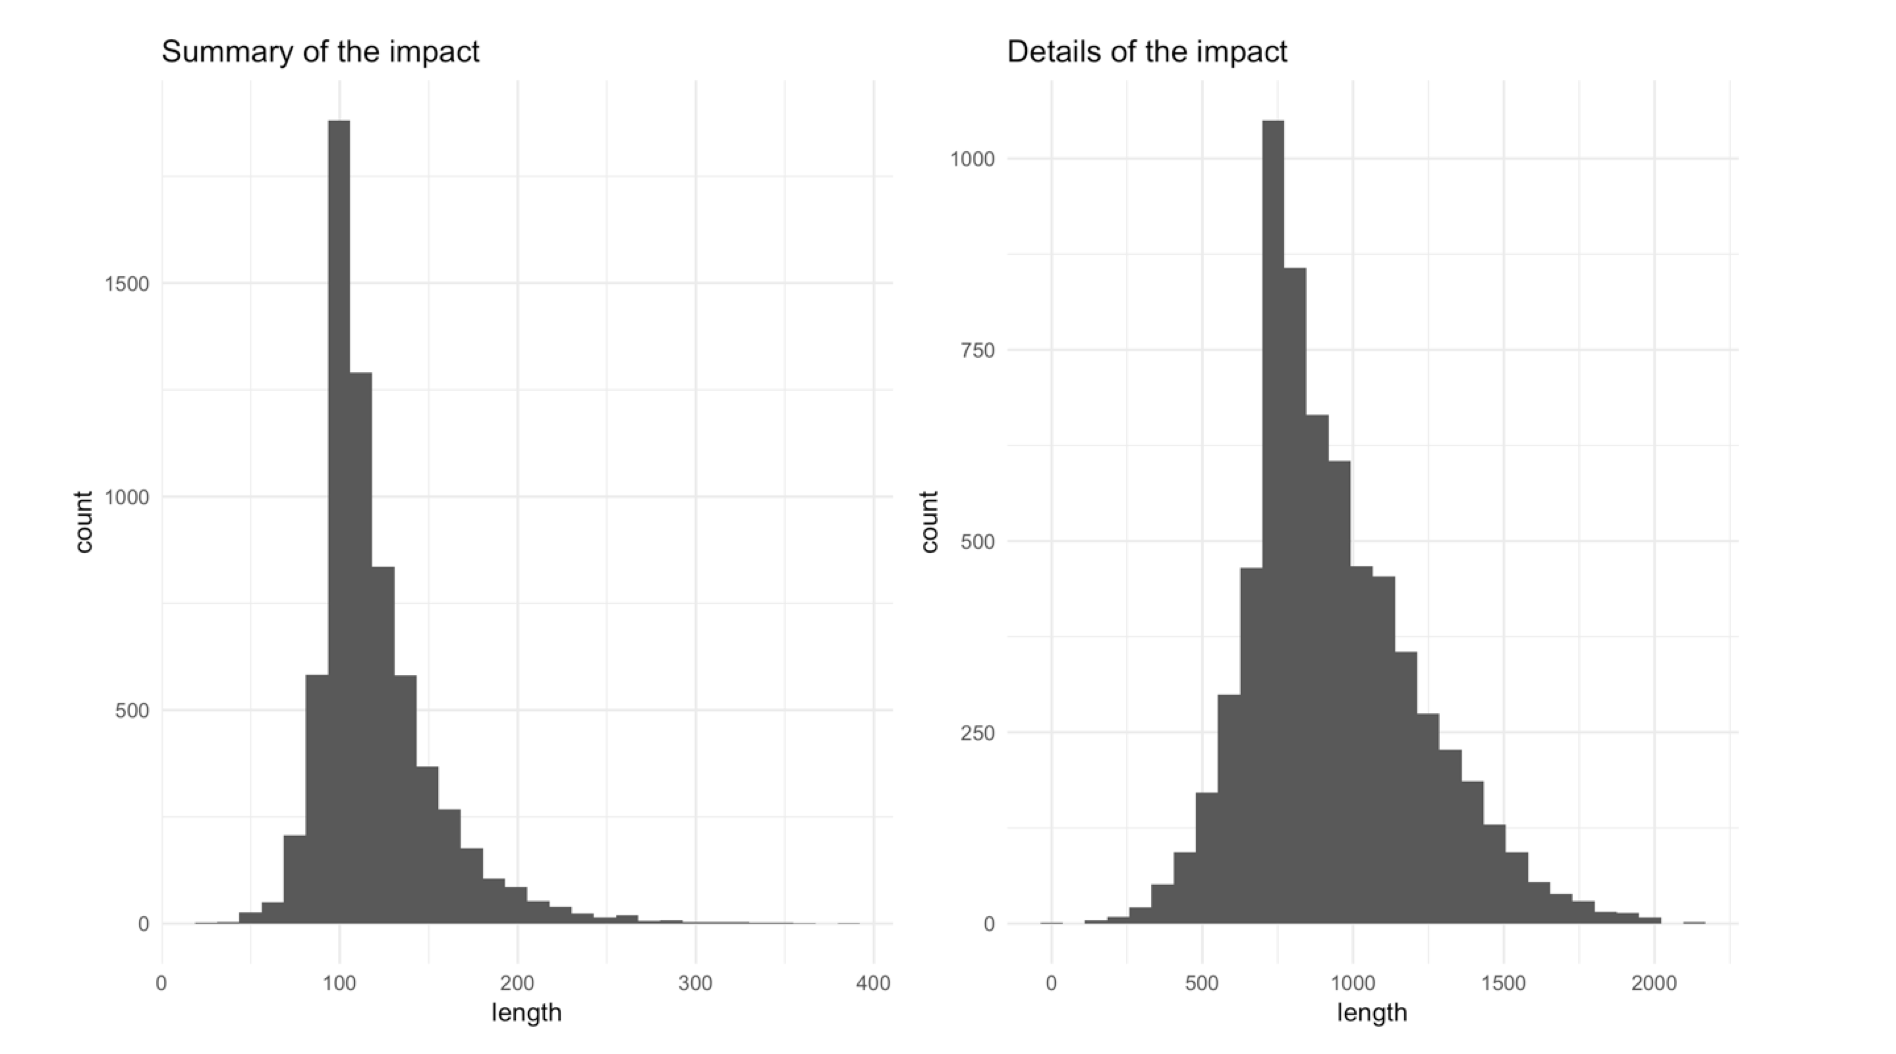
\includegraphics[width=1\linewidth]{_bookdown_files/figures/impact_histograms_length} 

}

\caption{Distribution of number of words in relevant sections of the REF impact case studies.}\label{fig:impacthistogramslength}
\end{figure}

Within the REF repository projects are classified using three criteria:

\begin{itemize}
\tightlist
\item
  Impact type: There are eight Summary Impact Types. These follow the
  PESTLE convention (Political, Economic, Societal, Technological,
  Legal, and Environmental) widely used in government policy
  development, with the addition of Health and Cultural impact types.
\item
  Units of assessment (UOA): Institutions were invited to make REF
  submissions in 36 subject areas, called units of assessment (UOAs),
  each of which had a separate expert panel.
\item
  Research subject areas: The REF Impact case studies are assigned to
  one or more Research Subject Areas (to a maximum of three) by text
  analysis of the `Underpinning research' (Section 2 of the Impact case
  study template). This is a guide to text search that uses a
  disciplinary structure that is more fine-grained than the one in the
  36 Units of assessment.
\end{itemize}

Figure \ref{fig:impactmetadataanalysis} shows the number of documents
per Unit of assessment.

\begin{figure}

{\centering 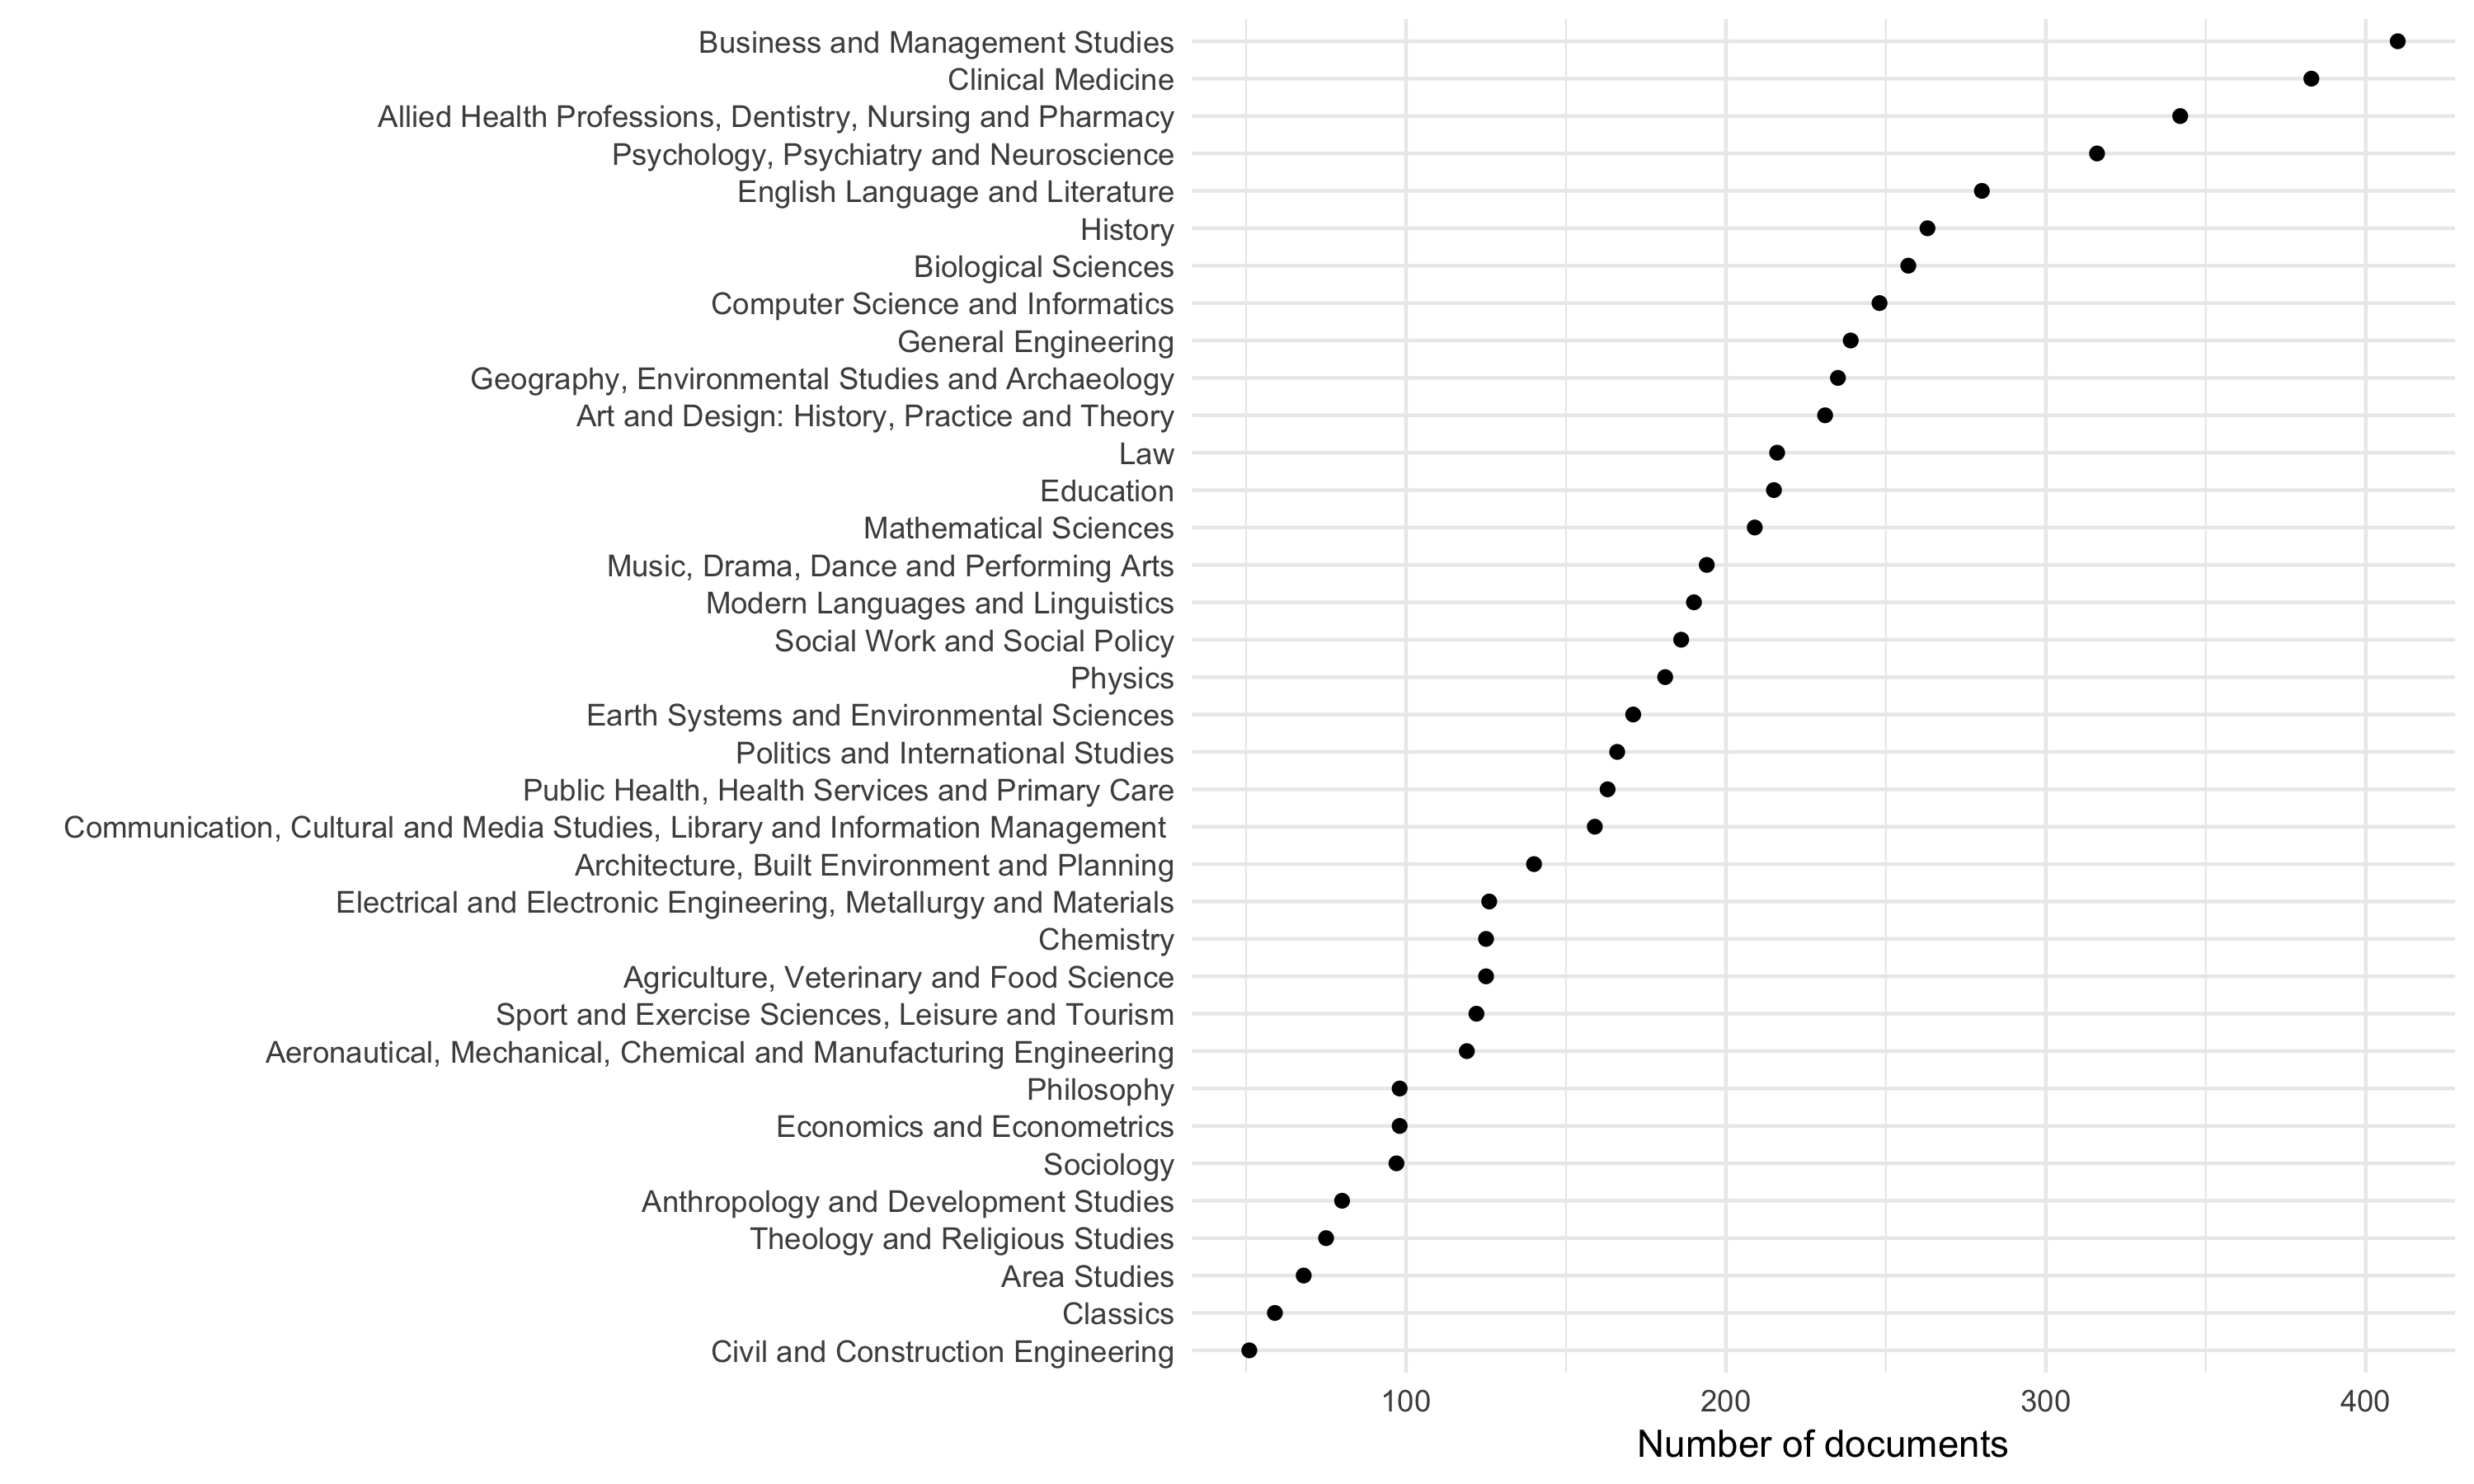
\includegraphics[width=1\linewidth]{_bookdown_files/figures/impact_metadata_analysis} 

}

\caption{Number of documents per Unit of assessment (UoA) in REF impact case studies.}\label{fig:impactmetadataanalysis}
\end{figure}

\subsection{Preliminary analysis of the
corpus}\label{preliminary-analysis-of-the-corpus}

In this section we present a descriptive analysis of the content of the
documents to give an evidence of two important facts: 1. The description
of the impact contains target groups; 2. This information is enough to
make a significant statistical analysis.

The corpus contains 8.230.598 words in total and 141.705 different
words. By annotating the entire corpus with the entries of the Enriched
dictionary we find that the total number of words referring to target
groups is 169.037, while the number of different target groups is 1830,
or 1.3\% of different words.The number of documents that contain at
least one target group is 6628, or 99,9\% of the total. Only for nine
documents we were unable to locate any word referring to a target group.

Figure \ref{fig:impactusersdistributions} offers a vivid demonstration
of the issue of specificity of words referring to target groups. As many
as 37\% of all projects include people, and as many as 25\% mention
company as isolated words. Among the top 20 occurrences we find
extremely generic words such as public, community, individual,
organization, user, or society. Slightly more specific are the words
referring to the school or youth context (child, school, student,
teacher) or the health context (patient, patients). In order to find
more specific words we have to go further down the ranking. Please note
that in all these cases these words do not appear in combination with
other that might increase the specificity, but in isolation. Should the
same word appear in combination with other more semantically connotated
words, they would form a separate target group. As an example, the word
people is considered part of a separate expression in the following
examples: people with cystic fibrosis, people with primordial dwarfism,
people with rheumatoid arthritis, ordinary people in extraordinary
situation, people in senior management, people from different
background, key policy people in UK government, specific community of
people, young people in deprived community in Glasgow. Each of these
expressions is considered as a separate target group and their
Specificity is computed according to the formula above.

\begin{figure}

{\centering \includegraphics[width=1\linewidth]{_bookdown_files/figures/impact_users_distributions} 

}

\caption{Top 20 occorrences of words referring to target groups in the corpus of REF impact case studies.}\label{fig:impactusersdistributions}
\end{figure}

To see the difference in the use of words in sentences consider the
following examples from REF case studies: ``The validation of the exit
poll forecast allowed people to see the power of social scientific
methods, and may have helped them to establish a level of trust in
evidence-based information'' (generic use of the word people) and ``Key
components of this are nurturing people with cross-cultural
understanding, diversity in thinking and global leadership skills''
(more specific use). The NLP procedure developed for this analysis is
able to accurately distinguish these situations.

\section{Results}\label{results-12}

\subsection{Descriptive analysis}\label{descriptive-analysis}

Table \ref{tab:impact2} offers a snapshot of the value of indicators
calculated across the entire corpus. The minimum value of indicators
(zero) is represented by the 9 documents without target groups. On
average the REF impact case studies contain words that represent target
groups as 2\% of total words, and words that represent distinct target
groups as 2.5\% of different words. In absolute terms, the median REF
impact case study contains 10 different words that refers to target
groups, repeated 22 times in total.

\begin{table}

\caption{\label{tab:impact2}Descriptive statistics of indicators of target groups in the corpus of REF impact case studies.}
\centering
\begin{tabular}[t]{lrlllll}
\toprule
Indicator & Min & Max & 1st quartile & 3rd quartile & Mean & Median\\
\midrule
Frequency:indicator & 0 & 9.2 & 1.2 & 2.7 & 2 & 1.9\\
Frequency: absolute value & 0 & 115 & 14 & 34 & 25469 & 22\\
Diversity: indicator & 0 & 7.6 & 1.8 & 3.2 & 2.5 & 2.4\\
Diversity: absolute value & 0 & 34 & 7 & 14 & 10518 & 10\\
Specificity & 0 & 1 & 0.59 & 0.731 & 0.659 & 0.656\\
\bottomrule
\end{tabular}
\end{table}

There is not large variability in the number of different target groups,
as the first and third quartile at 7 and 14 are close to the median
value. Interestingly, all distributions are close to the normal. A small
number of documents use words that refer to target groups with much
larger frequency and diversity. The document with maximum use of target
groups identifies as many as 34 different words or combination of words.
In terms of repetition, the document with the largest number of words
uses 115 times a word representing target groups. When coming to
specificity, the mean value of 0.659 implies a good level of
specificity, given the range of the indicator. Figure
\ref{fig:impactusersfreqcomparison} shows the distribution of documents
by indicators.

\begin{figure}

{\centering \includegraphics[width=1\linewidth]{_bookdown_files/figures/impact_users_freq_comparison} 

}

\caption{Top 20 occorrences of words referring to target groups in the corpus of REF impact case studies.}\label{fig:impactusersfreqcomparison}
\end{figure}

\subsection{Findings by subject area}\label{findings-by-subject-area}

We disaggregate the indicators with respect to the subject areas, or the
Units of assessment (UoA), according to the REF nomenclature. This
analysis offers a new perspective on the way in which he various
disciplines describe their impact pathways. We use the conventional
boxplot representation.

Figure \ref{fig:impactfrequency} shows a surprising finding. On top of
the ranking by frequency of occurrence of words that refer to target
groups of users we find Humanities: not only Education (which by nature
refers to children, students and teachers as user groups), but also
Music and drama, Classics, Language and literature, and History. Or, in
other words, disciplines that are not oriented towards users, but rather
cultivate the goal of knowledge per se. At the bottom of the ranking we
find, again surprisingly, Engineering disciplines, with a number of
specializations, and Economics, that is, disciplines that, on the
contrary, have a pragmatic orientation towards various target groups of
users.

\begin{figure}

{\centering \includegraphics[width=1\linewidth]{_bookdown_files/figures/impact_frequency} 

}

\caption{Boxplot of the Frequency indicator in the corpus of REF impact case studies by subject area (Unit of assessment)}\label{fig:impactfrequency}
\end{figure}

Figure \ref{fig:impactdiversity} confirms a similar ranking by subject
area when we use the Diversity indicator, with slight variations. In the
case of diversity we find also Theology and religious studies, as well
as Art and design. Almost all subject areas in Humanities consistently
show up at the top when we investigate the frequency by which they
mention users of research and the number of different target groups they
are able to identify. This is a remarkable finding. It is true that this
comes from documents that are themselves retrospective reconstruction of
impact, but this feature applies to all subject areas in the same way.

This finding sheds light on one of the controversial issues in the
literature on impact evaluation, that is, the role of Humanities and
Arts. It seems that one of the tenets of the argument that Humanities
and Arts are not sensitive to the audiences, or users, of their research
results, is simply false. When asked to reflexively reconstruct their
impact, they are systematically able to mention their target groups.

\begin{figure}

{\centering \includegraphics[width=1\linewidth]{_bookdown_files/figures/impact_diversity} 

}

\caption{Boxplot of the Diversity indicator in the corpus of REF impact case studies by subject area (Unit of assessment)}\label{fig:impactdiversity}
\end{figure}

This comes at a cost, however. Humanities rank top in the Frequency and
Diversity of target groups, but rank at the bottom when coming to their
Specificity. Figure \ref{fig:impactspecificity} shows an almost reverse
ranking of subject areas when the indicator chosen is Specificity. At
the top of the Specificity ranking we find Social Sciences, such as
Economics, Politics, Anthropology and Law. This is another interesting
finding. These disciplines have been able to target highly specific
groups of users, following a process of academic specialization. They
have low Frequency and low Diversity- that is, do not spend much
emphasis on their target users, but have high Specificity- that is, they
know whom to target.

Large part of Humanities are found at the bottom: Psychology, Education,
Philosophy, Language and literature, Art and design. Engineering
disciplines are more scattered.

Finally, by combining the three indicators it is possible to examine
more closely the pattern of impact of subject areas.

\begin{figure}

{\centering \includegraphics[width=1\linewidth]{_bookdown_files/figures/impact_specificity} 

}

\caption{Boxplot of the Specificiy indicator in the corpus of REF impact case studies by subject area (Unit of assessment)}\label{fig:impactspecificity}
\end{figure}

Frequency and Diversity are highly correlated
(\ref{fig:impactfrequencydiversity}). Humanities rank top in both
indicators and are located in the top right region of the graph. Almost
all disciplines in Engineering and Economics and Econometrics lie at the
opposite corner. When coming to Specificity, correlation with the other
indicators is on the contrary extremely low and is negative (- 0.016
with Intensity, - 0.146 with Diversity).

\begin{figure}

{\centering \includegraphics[width=1\linewidth]{_bookdown_files/figures/impact_frequency_diversity} 

}

\caption{Scatterplot of the relation between Frequency and Diversity indicators in the corpus of REF impact case studies by subject area (Unit of assessment)}\label{fig:impactfrequencydiversity}
\end{figure}

\section{Discussion}\label{discussion-1}

The data show an intriguing disciplinary pattern: Humanities and Arts
show remarkably higher frequency of terms related to users, but a
significantly lower specificity. The opposite is found for many areas of
STEM, namely Engineering and several Natural science disciplines.

The results for Humanities are very intriguing. Research in Humanities
is often considered as pure, abstract, not engaged with society. This
representation is used by those governments that argue that research
funding in these areas should be cut because their impact on society
cannot be demonstrated. For Social Sciences the situation is slightly
different, but there is a presumption that only a few social sciences
have an impact, in particular those with instrumental value, such as
Economics. Our data tell a different story. When asked to demonstrate
the impact of their research, scholars in Humanities and Arts use a very
rich vocabulary of users and mention users very frequently, twice as
much as scholars in STEM. At the same time, they are less capable to
transform their orientation in operational terms, by defining,
identifying, targeting specific groups or audiences. At the opposite
extreme, it seems that scholars in STEM mention very precise and well
defined groups of users. This might be a result of the nature of their
studies: researchers in Medicine follow specific targets in terms of
disease and patients, or technologists have narrow industrial
applications. This remarkable difference may create an imbalance in the
assessment of research impact.

Research in STEM finds more easily and unambiguously the groups of
potential users, so that its impact is easier to observe and
operationalize. As it has been noted by the studies on REF, evaluators
may find it easier to use concepts drawn from STEM to evaluate all types
of research, simply because they point to more observable and discrete
products of research. From the field of social studies of evaluation it
is well known that measurements lead to a feedback loop so that the
immediate availability of indicators may lead to believe that important
things are only those that can be measured.

The notion of impact of research deserves further and intense research
effort in the near future. We see several directions of research. First,
apply the methodology to ex ante research documents, such as research
proposals: do they include users? do they identify target groups with
adequate Diversity and/or Specificity? Second, test whether there is a
relation between the Specificity of identification of target groups and
the assessment of the research, either ex ante (approval of a proposal)
and ex post (score obtained in research assessment exercises). Third,
extend the methodology to other kinds of documents.

\chapter{Defining Industry 4.0 Professional
Archetypes}\label{defining-industry-4.0-professional-archetypes}

Worldwide industrial systems are evolving by leveraging Internet
connected technologies to generate new added values for organizations
and society. Researchers, policy makers and entrepreneurs refer to such
phenomenon with the name of Industry 4.0.

An increasing number experts from different fields are focusing on this
topic, bringing their contribution in terms of new technologies and
methods. As a consequence of this process, the companies that are
embracing the new paradigm need to manage new technologies and the new
relations among them with a multidisciplinary approach. The result is an
emerging need of new professional figures able to bridge the different
fields.

Moreover, while the scientific interest in technological aspects of
Industry 4.0 is constantly growing, the understanding of the future
works and professional roles is slowed down by the heterogeneity,
complexity and static nature of job description systems. These issues
are usually addressed by qualitative methods thus making the results
uncertain and partial.

The first step of the present chapter is to develop a data driven
mapping of 4.0 competencies which benefit (rather than being
disadvantaged) by the heterogeneity of the entities to map. Then we
propose a classification of the groups of competencies with the aim of
identifying and defining the archetypes of Industry 4.0 workers. Given
the bottom-up process we adopted to reach our goal, also the
relationships between them can be described.

\section{Digital Competences
Development}\label{digital-competences-development}

The radical technological change is going to affect the whole industrial
environment and will radically transform, in several different ways, the
world we live in (see section \ref{technimetrochap}). Consequently, the
revolution is not just referred to the availability of new sophisticated
machines, but also to the deep reconsideration of worker roles it brings
with. On the one hand Industry 4.0 implementation may have negative
impact on specific professional figures, which could be substituted by
robots. In support of this theory, Osborne \& Frey implemented a
methodology to estimate the probability of job computerization using a
Gaussian classifier \citep{frey2017future}. The results are quite
pessimist: they distinguished between High, Medium and Low risk of
computerization: according to their estimates around the 47\% of jobs is
in the high risk category. On the other hand, another possible impact is
represented by a significant increase of worker competences and the
emersion of new professional profiles: our research mostly focused on
the second prospect.

\section{Methodology}\label{methodology-12}

In this chapter we show the process to built the graph of Wikipedia
pages related to Industry 4.0. This graph will be then used by expert to
define 4.0 workers archetypes. Figure 1 shows the process we adopted.
The whole process takes in input a set of linked entities
(e.g.~Wikipedia pages) and gives as output a clustered graph.

\begin{figure}

{\centering \includegraphics[width=1\linewidth]{_bookdown_files/figures/archewf} 

}

\caption{Flow diagram of the process of 4.0 Archetypes definition.}\label{fig:archewf}
\end{figure}

\subsubsection*{Wikipedia Pages
Collection}\label{wikipedia-pages-collection-1}
\addcontentsline{toc}{subsubsection}{Wikipedia Pages Collection}

The process takes as input a set of entities linked between them. A link
between two entities represent the existence of a relation between them.
Here the concept of relation is intended as the sharing of a topic. In
other words, two entities has to be connected if they belong to the same
topic. Any entities-links structure that meets this requirements can be
used as input for the proposed process. For the purpose of the present
work, we decided to use the free encyclopedia Wikipedia . Wikipedia is
structured in such a way that each page contains links to other
Wikipedia pages. The links from page to page are manually assigned by
the contributors, so the structure of the links evolves dynamically.
Furthermore each page is labeled by the contributors through categories
with the intent of grouping together pages on similar subjects. To
collect industry 4.0 related wikipedia pages we exploit this information
and structure. In the date of 23/11/17 we collected three levels of
pages typologies for a total of 4739 pages:

\begin{itemize}
\tightlist
\item
  L1, The Wikipedia page of industry 4.0 \footnote{\url{https://en.wikipedia.org/wiki/Industry_4.0}}
  \emph{(1 page)}
\item
  L2, All the pages linked to L1 \emph{(39 pages)}
\item
  L3, All the pages linked to L2 \emph{(4699 pages)}
\end{itemize}

For each page we collected the page name, the links and the categories.

\subsubsection*{Pages Graph Generation}\label{pages-graph-generation}
\addcontentsline{toc}{subsubsection}{Pages Graph Generation}

Once we collected all the pages and the links between them, we represent
this structure as a directed graph (S). It is composed of:

\begin{itemize}
\tightlist
\item
  A set of nodes (N): the Wikipedia pages.
\item
  A set of edges (E): the links between the pages (considering also the
  direction of the edge)
\end{itemize}

S has 4739 nodes and 194.299 edges.

\subsubsection*{Nodes filtering on 4.0
Categories}\label{nodes-filtering-on-4.0-categories}
\addcontentsline{toc}{subsubsection}{Nodes filtering on 4.0 Categories}

Considering the content of Wikipedia, it is reasonable to assume that
not all of the 4.739 pages are related to Industry 4.0.

To sanitize the set of nodes N we adopted a series of filtering rules
based on the categories of the pages. The steps we followed were:

\begin{itemize}
\tightlist
\item
  Count the occurrence of each category we extracted. At this step we
  had 14.711 categories.
\item
  Filter the categories having an occurrence minor or equal to 3. This
  threshold level has been chosen looking at the distribution of the
  occurrences (the number of pages per category). A change in the
  central node could make changes on the selection of this threshold
  level. At this step we had 1.605 categories.
\item
  Manually screen the categories and select those related to industry
  4.0, taken in to consideration the definition of Industry 4.0. At this
  step we had 337 categories.
\item
  Selecting the nodes that contains at least one of the 337 categories.
\end{itemize}

As an example, the top 10 categories in terms of occurrence and the
relative occurrences are: production and manufacturing (51), parallel
computing (42), manufacturing (37), business terms (33), management
(31), process management (29), engineering disciplines (28), internet of
things(28), technology in society (26) and cloud computing (25). This
list shows how the process is able to make categories correlated to
Industry 4.0 emerge. We thus obtain a new graph S' that is a subgraph of
S (all the nodes N' and the edges E' are a subset of N and E
respectively). S' has 645 nodes and 703 edges. Of these nodes 75 are
disconnected from the graph (both in-degree and out-degree equals to
zero) and are thus not useful for the analysis we will conduct in
section 3.4 . These nodes are filtered, obtaining a definitive S' having
570 nodes.

\subsubsection*{Clustering}\label{clustering-2}
\addcontentsline{toc}{subsubsection}{Clustering}

We can assume that S' gives us a reasonable representation of Industry
4.0 related Wikipedia pages in terms of precision and recall.

It is thus possible now to analyze if the pages are arranged in
clusters, or in other words, if there exists groups of similar pages.

To understand the concept of similarity we need to consider the nodes N1
and N2, and the sets of all nodes connected to N1 and N2, respectively
L1 and L2. The similarity of N1 and N2 is proportional to the module of
the intersection between L1 and L2. To investigate this similarity and
to find clusters of similar pages, we grouped similar nodes via short
random walks \citep{durrett2007random}. The approach finds ways to
compute an intimacy relation between the nodes incident to each of the
graph's edges. The process is non-supervised so it makes an optimal
decision on the number of clusters. The output was 9 different
communities.

The obtained graph is shown in Figure \ref{fig:archeout}. The figure
shows the nodes, the edges and the label of the nodes. The dimension of
the nodes is proportional to the out-degree of each one (the number of
tail edges adjacent to the vertex) and the color represent the community
to which it belongs to. The label of the nodes (as center of the
clusters) are shown for those having an out degree greater than 4. The
table shows the correspondence between the community, the colors and the
percentage of nodes per community.

\begin{figure}

{\centering \includegraphics[width=1\linewidth]{_bookdown_files/figures/archeout} 

}

\caption{Representation of the graph S’. The nodes are the Wikipedia pages related to Industry 4.0. The arch between two nodes exists if there is a link between the pages. The labels of the nodes are shown only for nodes having an out-degree (number of tail edges adjacent to the vertex) greater than 4. The color of each node represent the community to which the node belongs. The table in the low-left shows the percentages of nodes for each community.}\label{fig:archeout}
\end{figure}

\subsubsection*{Workers 4.0 Archetypes
Definition}\label{workers-4.0-archetypes-definition}
\addcontentsline{toc}{subsubsection}{Workers 4.0 Archetypes Definition}

The authors generated a list representing the ``Industry 4.0 workers
archetypes'' based on Wikipedia. The bias due to the profile of people
writing this kind of Wikipedia pages does not reduce the importance of
this exercise, but it is fundamental to understand why the reader will
find such a great emphasis on technologies, methodologies and tools as
pages describing the archetypes in section 4. Skills, competences and
professional figures (in the strict sense) are then behind and beyond
the archetypes, which represent just the attitudinal profile of the
workers that will be soon seek by companies adopting Industry 4.0
paradigm.

Table of Figure \ref{fig:archeouttab} shows the relation between the
Archetypes and the communities (created by the text-mining procedure
presented above). It also shows the total number of nodes per archetypes
and per community.

\begin{figure}

{\centering \includegraphics[width=1\linewidth]{_bookdown_files/figures/archeouttab} 

}

\caption{Table of the accordance between the archetypes and communities. The total of pages for each archetypes is shown in the last column, the total of pages for each community is shown in the last row. }\label{fig:archeouttab}
\end{figure}

From this table it emerges that:

\begin{itemize}
\item
  Group 1 (75 pages) has two nodes/centers: the page ``Big Data'' and
  the page ``Analytics''. This is why from Group 1 derives two different
  Archetypes: ``the Architect'' (44 pages, centered in Big Data) and
  ``the Prophet'' (21, centered in Analytics). This is an evidence of
  the fact that these two archetypes are strongly related between them,
  since they belong differently from all the other groups.
\item
  More than 80\% of the pages referred to Group 2 (centered in the page
  ``SCADA'' and ``Industrial Control system) were used for creating the
  Archetype of ``the Perfectionist''. It is important to underline that
  the page SCADA - acronym of Supervisory control and data acquisition-
  being a specific control system architecture, was discarded from the
  assignation to a specific archetypes. Our focus for designing ``the
  Perfectionist'' was the generic page ``Industrial Control System''.
\item
  Group 3, Group 4 and Group 9 are composed of pages we linked to the
  same Archetype: ``The Geek''. In respect of Group 1, we made a
  different choice: we referred the most part of these three groups'
  pages to just one Archetype, ``nuanced'' on the basis of the nearest
  technologies in the graph: ``Cloud Computing'', ``Automation'' and
  ``Internet of Things''. As the Geek was created starting from three
  different groups, it has three different declinations as shown in
  Figure \ref{fig:archecoolout}. The geek, as will be explained in
  section 4, has to be seen as the expert of a specific family of
  similar technologies strongly related to industry 4.0.
\item
  Group 6 is composed of 26 pages, that were referred to almost all the
  Archetypes. These pages are general purpose, and referring to Figure
  \ref{fig:archeout}, this is also evident from their central position
  in the graph (there are related to every community). The predominance
  of pages referred to one Archetype (the Geek) did not allow us to
  consider this Group, centered in the page ``Computer Integrated
  Manufacturing'', as another nuance of ``the Geek''. Moreover, Group 6
  is strictly related to Group 9, as the proximity of the clusters in
  the graph can easily show.
\item
  In group 7, centered in ``Root Cause Analysis'' page, we found 100\%
  of pages referable to the Archetype we called ``The Investigator''.
\item
  As in the previous group, also in Group 8 (centered in ``Value Chain''
  page) the 100\% of pages were referable to one Archetype: ``the
  Strategist''
\end{itemize}

Figure \ref{fig:archecoolout} shows the same graph of Figure
\ref{fig:archeout}, associating to each group an Archetype. In this new
version of the graph it is possible to identify the centers of each
cluster, the position of the clusters (and the related archetype) in
respect of the others, the interrelation among the clusters/archetypes.

\begin{figure}

{\centering \includegraphics[width=1\linewidth]{_bookdown_files/figures/archecoolout} 

}

\caption{The different professional archetypes associated with each technological cluster.}\label{fig:archecoolout}
\end{figure}

\section{The Archetypes}\label{the-archetypes}

The term ``archetype'' has its origins in the Greek word ``archein'',
which means ``original or old'' and ``typos'' ``pattern, model or
type''. It is thus etymologically referred to the ``original pattern''
from which all other similar persons are derived, modeled or emulated.
In this work we consider this etymological meaning, discarding any
philosophical or psychoanalytic references which would mislead our
research. As regards the personality many theories have been proposed
over the years {[}11,12{]}, but a common vision at the academic level
has not been reached yet. Both Jung's theory of personality types
{[}13{]} and the Myers-Briggs indicator (MBTI) in the field of work
psychology {[}14{]} come to several psychological types defined through
descriptions and traits. Some of them (e.g.~the 16 psychological types
of MBTI) are a standard for Human Resource managers and are largely used
for resource classification and selection. It is important to underline
that in the present work i) technologies and skills have been extracted
in a scientific and repeatable manner, ii) they have been clustered
following a well-known and accepted algorithm. Conversely, archetypes'
names have been chosen with the intent to better communicate the
research outcomes.

The archetype description sections are built following a common
structure:

\begin{enumerate}
\def\labelenumi{\arabic{enumi}.}
\item
  \emph{The name of the archetype.} The choice of the name was made by
  the authors in order to have an evocative impact on the reader and
  reaching a communication goal. In some cases, the names are
  deliberatively imaginative, renouncing to respect a rigid scientific
  approach with the aim of charming and interesting the reader
\item
  \emph{The list of the Wikipedia pages selected.} The pages represent
  the elements considered by the authors for defining the archetypes.
  The selection of the pages was done referring to the clusters
  identified with the data-mining as shown in section 3. All the
  Archetypes are referred at least to one group, with the exception of
  group 1, from which two different Archetypes were created, and groups
  3,4 and 9, which all together participated in the creation of another
  Archetype (even if with three different declinations). In many cases
  the pages reported in the box are related to technologies,
  methodologies, tools: evidently the authors of Wikipedia pages related
  to Industry 4.0 are more interested in ``hard'' rather than ``soft''
  topics, such as competencies or cultural aspects of the new paradigm.
\item
  \emph{Industry 4.0 Emerging needs.} The authors presented shortly the
  needs that the companies face when introducing Industry 4.0
  applications. The needs are mainly based upon the interpretation given
  by the acatech study {[}15{]}, which represent one of the most
  effective key for understanding the new paradigm {[}16{]}.
\item
  \emph{The archetype.} We have already explained what we meant with the
  word ``archetype'' and the rationale behind the choice of the specific
  names. The explanation of the archetype given in this section is based
  on the interpretation of the Wikipedia pages selected and on the
  semantic fields they refer to. We tried to describe the inner nature
  of the individuals referable to each specific archetype, defining the
  peculiar traits of their mindset and their most marked features. The
  aim was also to describe them so to make them recognizable in our
  daily experience.
\item
  \emph{Keywords.} The keywords are taken from the column ``categories''
  of the clustered list of selected Wikipedia pages. Strikethrough in
  the body of the text indicates where the authors decided of deleting
  misleading words: we kept them for making clear and transparent the
  procedure behind this cleaning activity. The reasons for deleting some
  words were: a) they were too generic and did not characterize the
  archetype, b) they were too specific and they made the archetype
  losing its capacity of encompassing more aspects, c) even if they
  survived to the ``cleaning'' after the data-mining, they were referred
  to another semantic field (disambiguation).
\end{enumerate}

\subsubsection*{The Architect}\label{the-architect}
\addcontentsline{toc}{subsubsection}{The Architect}

\emph{The Wikipedia pages selected}: Big data; Data blending; Data
quality; Cognitive computing; Data fusion; Data science; Unstructured
data; Data lake; Data set; Data; Data lineage; Data transmission;
Radio-frequency identification; Data philanthropy; Datafication

\emph{Industry 4.0 Emerging needs}

When taking a decision in Industry 4.0 paradigm it is more important
than ever that the individuals can access, collect and process data and
information. Data can be gathered from machinery, equipment and tools
thanks to sensors, actuators and information processing systems, linked
to a communication layer. Big data is a buzzword usually linked to
Industry 4.0 and used to describe mass data that cannot be analyzed
adopting common procedures, but requires advanced applications and
technologies. Thus, in the new paradigm, it is important not just
collecting the data, but also collecting and processing them in an
innovative way and shaping them in a form that make them usable for the
company decision-makers and other employees.

\emph{The archetype: The Architect}

The Architect is the individual that is at ease in managing,
transforming and processing data. He/she has a clear idea of the
importance of data and understand which data are useful, in which
context and for who. The Architect likes formalized information and the
possibility of shaping them, has an innate capacity of breaking the
problems and find the best solutions: this capacity is fundamental when
having to deal with different sources of information and numerous data
and inputs. He/she is precise and reliable, has a great aptitude for
visualization and for problem solving.

\emph{Key words}: big data; data management; distributed computing
problems; technology forecasting; transaction processing, artificial
intelligence; cognitive science business intelligence; data; information
technology management, computer data, automatic identification and data
capture; privacy; radio-frequency identification; ubiquitous computing;
wireless, big data, types of analytics, online analytical processing

\subsubsection*{The Prophet}\label{the-prophet}
\addcontentsline{toc}{subsubsection}{The Prophet}

\emph{The Wikipedia pages selected}: Analytics; User behavior analytics;
Business analytics; Data mining; Data analysis; Continuous analytics;
Machine learning; Data visualization; Cultural analytics; Predictive
analytics; Natural language processing; Customer analytics; Business
intelligence; Analytic applications; News analytics; Statistics;
Behavioral analytics; Predictive engineering analytics

\emph{Industry 4.0 Emerging needs}

The implementation process of the Industry 4.0 paradigm involves
different stages. At one advanced stage of this process the company
should be able, starting from the data collected, to simulate future
scenarios and select the most likely one {[}15{]}. To do so the company
needs to have analyzed and assessed a number of data and projected the
``digital shadow'' of its assets in the future. Forecasting and the
recommendations based on it became the key elements on which building
the development of the company. The analysis of the different scenarios
is the basis for building the business success. For reaching these
targets it is fundamental to have constructed proper ``digital shadows''
of the assets and have understood the interactions among them.

\emph{The archetype: The Prophet}

The Prophet is an individual with strong analytical thinking skills,
able to examine in details specific situations in a critical way. He/she
has a future-oriented mindset: is at ease in thinking about next steps,
possible scenarios and with a medium-to-long-term vision. Starting from
the analysis of data and adopting also statistical methods, the Prophet
investigate the problems (creative thinking) and identify possible
solutions (complex problem solving) in order to reach the best case
scenario he designed.

\emph{Key words}: analytics; business intelligence; business terms;
financial data analysis; formal sciences; data mining; formal sciences;
cybernetics; learning; machine learning; actuarial science; big data;
business intelligence; financial crime prevention; prediction;
statistical analysis; types of analytics; financial technology;
information management; data; formal sciences; information; mathematical
and quantitative methods (economics); research methods; statistics;
artificial intelligence; computer security; human behavior; machine
learning; computational fields of study; data analysis; particle
physics; scientific method; data; information technology governance;
statistical charts and diagrams; visualization (graphic); artificial
intelligence; computational fields of study; computational linguistics;
natural language processing; speech recognition; business intelligence;
business software stubs; applied data mining; business analytics; market
research; marketing performance measurement

\subsubsection*{The Perfectionist}\label{the-perfectionist}
\addcontentsline{toc}{subsubsection}{The Perfectionist}

\emph{The Wikipedia pages selected}: Industrial control system;
Instrumentation; Control valve; Overall equipment effectiveness;
Enterprise resource planning; Distributed control system; Control
system; Lean manufacturing; Total productive maintenance; Programmable
logic controller; Risk; Control System Security; Control loop

\emph{Industry 4.0 Emerging needs}

Since the First Industrial Revolution, quality improvement has been one
of the critical aspects for developing any business. In the current age
of high competition and mass production, this has become, along with
price strategies, the main element for expanding the market. Thus,
quality control has become a central issue to consider before
establishing any industrial undertaking and the best way for ensuring
the best allocation of resources and highest level of production. In
Industry 4.0 paradigm quality has become even more important, mainly
because the increased flexibility of machinery, processes and procedures
allow to intervene continuously for analyzing the parameters, identify
machine faults or quality issues with a high degree of confidence and in
advance. Flexibility and agility (which denotes the ability to implement
changes in real-time, including changes to the company's business model)
are two key factors that allow a constant improvement.

\emph{The archetype: the Perfectionist}

The Perfectionist is the individual who is never satisfied of the actual
conditions: it could be his/her current personal situation, the
preparation for an exam, the functioning of a process or a machinery.
He/she always thinks that things can be done better, in a shorter time,
with less resources, involving different teams, collaborating more (or
less). The Perfectionist likes tests: he/she tries, monitors, checks the
results, thinks about it (possibly analyzing data and empirical results)
and then suggests - or decides - how to make things work right.

\emph{Key words}: control engineering; industrial automation; industry;
manufacturing; telemetry; lean manufacturing; automation; control
theory; systems engineering; systems theory; industrial computing;
programmable logic controllers; measuring instruments; sensors; business
terms; computer-aided engineering; erp software; enterprise resource
planning terminology; information technology management; management;
production and manufacturing; supply chain management terms; commercial
item transport and distribution; inventory; management; process
management; production and manufacturing; actuarial science;
environmental social science concepts; financial risk; risk;
applications of distributed computing; control engineering; industrial
automation; control devices; valves; applications of distributed
computing; control engineering; industrial automation; business terms;
commercial item transport and distribution; computer security; computer
security procedures

\subsubsection*{The Geek}\label{the-geek}
\addcontentsline{toc}{subsubsection}{The Geek}

\emph{The Wikipedia pages selected}: Cloud computing; Smart grid;
Productivity; Cyber manufacturing; Artificial intelligence; Embedded
system; Cyber-physical system; Cybernetics; system; Manufacturing;
Computer network; Cloud manufacturing; Computer security; Internet of
things; Information technology; Distributed computing; Service-oriented
architecture; Automation; Adaptable robotics; Automation Technician;
Developmental robotics; Industrial Engineering

\emph{Industry 4.0 Emerging needs}

Beside the aspects related to a new organizational structure and a
different work culture, Industry 4.0 is strongly determined by the new
technologies, both hardware and software. It is impossible to implement
Industry 4.0 applications without considering technical aspects. The
enabling technologies (Clouds, Augmented reality, Simulation, IoT, etc.)
must be known in the company in order to make the new paradigm real.
Technologies are so specific and so many, that it is important to have
an extensive knowledge of them (even if not deep) and be able to
integrate them for finding the most effective custom-made solution to
solve specific problems.

\emph{The archetype: the Geek}

The Geek is the archetype of an individual extremely passionate in new
technologies and its applications. He/she is interested in everything is
new and innovative, in seeing beyond and within things: how
technological applications work, why and at what extend their capacities
can be brought. Integration is always an important aspect: the Geek
appreciate the ideas of combining, breaking and keeping just some
aspects for recombining and then creating something new. He/she has a
kinesthetic learning (or tactile learning) and has a kinesthetic
approach to the work: he/she needs make tests (rather than thinking or
planning), piloting solutions (rather than have someone else doing the
job) and working on the field. The geek is always up-to-date on the
newest technology and is always willing to be the first in creating
something new. As the number of pages referable to the Geek were
numerous, the authors decided to create three different nuances
represented by three different logos, one for each field of expertise of
the Geeks.

\emph{Key words}: ambient intelligence; emerging technologies; internet
of things; computers; information-theoretically secure algorithms;
information technology; media technology decentralization; distributed
computing; architectural pattern (computer science); enterprise
application integration; service-oriented (business computing); software
design patterns; web services; cloud computing; cloud infrastructure;
big data; industrial revolution; industrial automation; industrial
computing; technology forecasting; computer systems; industrial
computing; industry; internet companies; manufacturing; computer
systems; physical systems industry; manufacturing ambient intelligence;
emerging technologies; smart grid; artificial intelligence;
computational fields of study; computational neuroscience; cybernetics;
formal sciences; technology in society; unsolved problems in computer
science; cybernetics computer networking; computer networks;
telecommunications engineering; computer network security; crime
prevention; cryptography; cybercrime; cyberwarfare; e-commerce;
information governance; national security; secure communication;
security technology; weapons countermeasures; economic growth; industry;
production and manufacturing; production economics; electrical
engineering; embedded systems; cloud computing; automation; engineering
disciplines; adaptable robotics; robot kits; robotics stubs; industrial
automation; technicians; machine learning; robot control; engineering
disciplines; industrial engineering; operations research; production and
manufacturing

\subsubsection*{The Investigator}\label{the-investigator}
\addcontentsline{toc}{subsubsection}{The Investigator}

\emph{The Wikipedia pages selected}: Root cause analysis; A3 problem
solving; Failure mode and effects analysis; Quality control; Business
process mapping; Forensic engineering; Business process; DMAIC; Incident
management; Value stream mapping; Design of experiments; Pareto chart;
5S (methodology)

\emph{Industry 4.0 Emerging needs}

Industry 4.0 paradigm enables to a constant check on procedures,
processes and systems, as they are all integrated and all the
information are conveyed to a same ``repository'' (the communication
layer). All these aspects can be then monitored in a totally new way: it
is possible, for example, to have data in real time and the decisions
can be taken according to information which can be transferred almost at
the same time they are created by one or more devices or tools. Thanks
to the high amount of information than can be analyzed, also mistakes
can be treated in a different way: in Industry 4.0 it becomes easier to
focus and investigate on the causes of a failure -- and solve it -,
rather than on finding out who is to blame.

\emph{The archetype: the Investigator}

The Investigator is the individual who is naturally curious: as a proper
scout he/she wants to understand what is working and what is not. He/she
is never satisfied with the explanation he/she receives and is always
searching for a mistake, a bug or just another way for reaching at the
same conclusion. The Investigator is eager for analyzing what is already
known and what is new, he/she likes going into details and understanding
how things works and how they could work in a different way. When
identified the problem the Investigator is not necessarily interested in
finding the fix, he/she rather prefer to have some other problems to
break and leaving someone else the possibility of coming up with a
solution (that he/she would love to analyze again).

\emph{Key word}: business terms; problem solving; process management;
production and manufacturing; quality; quality management; six sigma;
design for x; management; quality control; statistical process control;
business process; enterprise modelling; process management; lean
manufacturing; commercial item transport and distribution; inventory;
japanese business terms; lean manufacturing; manufacturing; methodology;
process management; quality control tools; business process; data
management; design of experiments; experiments; industrial engineering;
quantitative research; statistical theory; systems engineering;
reliability analysis; reliability engineering; systems analysis;
engineering disciplines; engineering failures; forensic disciplines;
materials science; business software; disaster preparedness; enterprise
modelling; firefighting in the united states; itil; incident management;
categorical data; statistical charts and diagrams

\subsubsection*{The Strategist}\label{the-strategist}
\addcontentsline{toc}{subsubsection}{The Strategist}

\emph{The Wikipedia pages selected}: Value chain; Core competency; SWOT
analysis; Business model; Delta Model; Strategic management; Balanced
scorecard; Game theory; Strategic planning; Control (management);
Porter's five forces analysis; Strategic thinking

\emph{Industry 4.0 Emerging needs}

If Industry 4.0 allows the companies to foresee different scenario based
on data and information, it doesn't not guarantee to the entrepreneurs
to select the right one or take the correct decision. Data should be
read correctly, but also the strategy for reaching the preferred
scenario should be decided in the proper way. In particular, one of the
most dangerous risk is not being able to redefine properly the company
business model, which should be constantly monitored, assessed and,
according to the most updated information, modified.

\emph{The archetype: the Strategist}

The Strategist is the individual who has a mind wide open: he/she thinks
to the outcomes of each activity and reflect on the different ways for
reaching the target. Strategic thinking, strategic management and
planning are its most marked qualities: he likes thinking to all the
possible outputs in a comparative way. He/she is also a pragmatist, as
starting from the analysis of the current situation he/she doesn't like
to create different scenarios (as the Prophet does) but rather reaching
the result established in the more effective way. Even if the Strategist
is not an entrepreneur, he has some of its qualities and this is why
this archetype can be referred to the ``entrepreneurial mindset''. The
Strategist is visionary, risk-taker, creative, with a strong willingness
to challenge the status quo and he has diplomatic and leadership skills.

\emph{Key words}: distribution (business); michael porter; process
management; supply chain management; value proposition; business models;
management; strategic management; types of marketing; business planning;
business software; business terms; management; control (social and
political); control theory; artificial intelligence; formal sciences;
game theory; john von neumann; mathematical economics; business terms;
strategic management; business intelligence; strategy; systems thinking

\section{Discussions}\label{discussions-1}

The present section can be seen as a first step of a long journey. As
stated in introduction our Archetypes are intended in the etymological
sense, as original models, and we assume that they are emerging in the
digital economy. Thanks to the data-mining exercise we were able to
place the clusters of Wikipedia pages in a graph, analyzing them
according to the contents, the position in the graph and the relation
among them. This recurrence of same pages in almost all the clusters let
us concluding that some topics are common to all the Archetypes,
independently to the cluster they were originated. For example, being
able to read and exploit data is a transversal issue and all the
Archetypes (and all the workers referable to them) should be used to
work with them. Another constant in all the cluster is the reference to
technologies: they are central in the new paradigm, it is unavoidable
for a digital worker knowing them. Even if the ``Fourth Industrial
Revolution'' doesn't end with a bunch of IT tools, they are at the
center of the new paradigm and workers must be used to play with them
{[}17{]}.

To conclude and anticipate the further developments, in figure
\ref{fig:archeporter} we give an interpretation of the position of the
archetypes in the graph. We can cluster the Archetypes according to the
general company area they could be referred. The areas are:

\begin{enumerate}
\def\labelenumi{\arabic{enumi}.}
\tightlist
\item
  Business. The Strategist and the Investigator are the main actors. In
  this area the decision regarding the future and the strategy of the
  company are taken: it is important to have people who have always the
  big picture clear in their mind (the Strategists) and are good in
  analyzing the situation for what it is (the Investigator).
\item
  Data. The Architect and the Prophet suits well here. This area is
  referred to the acquisition, collection and management of data. This
  area is perfectly suitable for someone who is comfortable in analyzing
  and structuring data (the Architect) and for who has a future-oriented
  mindset, always based on the actual inputs coming from the company
  functions (the Prophet).
\item
  Process. The Geek (automation) is the only major player in this area.
  The process area is where the core activities of a company are
  performed.
\end{enumerate}

The connection between the three areas are ensured by three Archetypes:

\begin{itemize}
\tightlist
\item
  The Perfectionist, is the bridge between the process area and the
  business area: in both of them is useful to have someone who is
  comfortable in solving problems and making things work always better.
\item
  The Geek (cloud) is the bridge among the Data area, where he/she
  contribute with the knowledge of technologies, and the Business area,
  where Archetypes will benefits from these technologies for new
  business development.
\item
  Finally, the Geek (IoT) is the connection among the Process area and
  the Data area, representing the bridge between the core activities and
  the usage of information coming from them.
\end{itemize}

A possible next step of our study will be identifying at which function
of the Porter value chain model each Archetype suits better. Then,
having placed the Archetypes in their most suitable function, it will be
then possible to allocate for each Archetype the most appropriate 4.0
professional profiles, so to follow their attitudes and exploit better
their skills. At this stage, as the new paradigm is still emerging, we
cannot go further in our research, but the road-map is now clear and the
first step is taken.

\begin{figure}

{\centering \includegraphics[width=1\linewidth]{_bookdown_files/figures/archeporter} 

}

\caption{The Archetypes grouped by business areas. The image also shows the strategic roles of Perfectionist, Cloud Geek and IOT Geek, who represent the bridges between different functions.}\label{fig:archeporter}
\end{figure}

\part{Conclusions}\label{part-conclusions}

The thesis has faced the problem of Mining Technical Knowledge from
documents with a particular focus on Engineering Management Methods and
Natural Language Processing Techniques. Its main goals are three:

\begin{itemize}
\tightlist
\item
  understand which information sources contain the most untapped value
  and which methods and tools can be used to uncover that.
\item
  understand how management engineering can cover those areas.
\item
  designing analysis algorithms, which can provide correct knowledge
  exchange between human and machine, leading to incorporate knowledge
  of the experts inside machine-learning systems and improve the usage
  that experts' makes of machine outputs in their process of decision
  making.
\end{itemize}

The designed solutions make large use of the Design Science Approach,
the Data Science Workflow and Natural Language Processing Techniques.

In \emph{Part Number 2 ``State of the Art''} has made a review of tools
and techniques for Natural Language Processing and shows the documents
used for knowledge extraction. In particular, the analysis of technical
documents require the design of processes that rely both on Natural
Language Processing techniques and on technical field expertise. While
the first techniques are codified and explicit, the second are sometimes
implicit and always hard to systematize. In the State of the Art these
two groups of techniques are treated in the same way to give to the
reader a systematic literature review on these topics. Furthermore it is
important to define the value in terms of new knowledge that documents
can bring to companies. The goal of this state of the art is to
demonstrate that a large literature on Techniques able to solve the
problems discussed in section \ref{introproblems} exists, but week or no
effort exist in the literature in the systemic integration of these
tools and in the design of holistic methods to solve these problems.

\emph{Part Number 3 ``Methods and Results''} has been the core Part of
the thesis. This part describes the methods and processes designed for
the analysis of technical documents following the guidelines of design
research described in section \ref{introdesres}. Since design research
is a problem solving paradigm, each chapter (focalised on a different
kind of document) starts with a brief description of the field of
application of the method and with the framing of the problem to be
solved. Then the methodology to solve the problem is described with the
goal of being clear to a technical audience and a managerial audience.
Each chapter closes with the results description that proves the
utility, quality, and efficacy of the design artifact.

\emph{Part Number 4 ``Applications of the Results''} is a collection of
projects that describes the applications and results of the methods
designed in \emph{Part 3 ``Methods and Results''}. The goal, again
following the the guidelines of design research
\citep{bichler2006design}, is to provide clear and verifiable
contributions in the areas of the design artifact, design foundations,
and/or design methodologies.

In this Part a brief summary of the thesis is made, and its future
developments are described. Before that, a more descriptive-science view
of the results is given. In the next chapter we give a general method
that has proven to be effective in the major part of the designs of the
present thesis: \textbf{lexicons design}.

\chapter{Lexicons Design for Mining Technical
Knowledge}\label{sotadocumentsunderstandlexicons}

In this work as been shown that text mining techniques are being adopted
in many different fields to face the problem of extracting meaningful
information hidden in unstructured data. Hybrid processes
(human-machine) of knowledge extraction are usually the best solution
for companies to achieve great results and to ensure the conformity of
the output of the knowledge extraction process. Anyway, state-of-art
literature on Natural Language Processing (NLP) lacks in process
management studies. In particular, researchers have not yet studied the
best way to integrate NLP outputs with human activities. To our best
knowledge, the present thesis is a first step in the desired direction.
Such a process and the design of new methods for human-machine (or
better engineers machine) interaction , started with the present thesis,
bring some valuable contribution to the literature:

\begin{itemize}
\item
  Minimize the introduction of errors and biases made by human
  intervention;
\item
  Maximize the human effort only on value added tasks such as knowledge
  validation and consolidation;
\item
  Decrease the overall time of the process.
\end{itemize}

From this thesis emerges the fact that \emph{Information Extraction from
texts for developing technical dictionaries (a Knowledge Base), is a
effective approach to follow in order to increase the knowledge base of
a specific field.} Many of the designs presented in this thesis uses
this approach.

In section \ref{usersresults} a dictionary of \emph{users of inventions}
has been developed, containing more than 76.000 entries, and this
dictionary has been used to analyze projects texts \ref{impactresuser}.
In section \ref{advdrwresults} a dictionary of \emph{advantages and
drawbacks} has been extracted from patents using twitter to validate its
content. The dictionary contains a total of 6.568 advantages and the
14.809 drawbacks and has been used to classify problems of different
technologies in patents \ref{explpatentnovel} and papers
\ref{blockchainanalysis}. This dictionary has also been used to design a
novel technical sentiment analysis, which has been used to analyze the
sentiment about two innovative products in section \ref{techsentanal}.

Sections \ref{smtextdrivenbottomup}, \ref{precisionagri} and
\ref{technimetrochap} developed dictionaries for respectively
sustainable manufacturing, precision agriculture and industry 4.0 with
the aim of giving a clear picture to both academics and practitioners
about the state of the of art of technologies in these fields. In
particular in section \ref{technimetrochap} the dictionary is an
enriched dictionary: the enriched dictionary can be defined as a set of
enabling technologies for industry 4.0, associated to their definitions
and to the linkages between them.

In this final chapter of the thesis we give a descriptive-science view
of the results. We thus present a general method that has proven to be
effective in the major part of the designs of the present thesis:
\textbf{lexicons design}.

\section{The Knowledge Bases and Technical
Lexicons}\label{the-knowledge-bases-and-technical-lexicons}

A Knowledge Base is an organized repository of knowledge - in a computer
system or an organization - consisting of concepts, data, objectives,
requirements, rules, or specifications. Technical Lexicons (or
Dictionaries) are lists of keywords and expressions linked to a specific
topic and they are used to extract information through the research of
these keywords in raw texts. All the methods that use these lists of
keywords are named Dictionary-based Approaches.

For using these approaches, the first thing to do is the construction of
these dictionaries. For some applications - i.e.~biomedical fields -
there are already existing dictionaries that can be used for text
mining; in other applications, these dictionaries need to be
constructed. The development of dictionary is a task still too
human-dependent: in fact, for building these lists, domain experts must
select keywords from texts and clear them from words that are too
general for that domain; this process must be repeated iteratively until
a satisfactory result is achieved, in relation with the purpose. These
tasks rely too much on the intervention of experts and the subsequent
analysis are greatly influenced from their choices and opinions. Experts
intervention is also too time consuming and expensive.

Another way to increase the Knowledge Base is through the Named-Entity
Recognition Techniques. Named-entity recognition (NER) - also known as
entity identification, entity chunking and entity extraction- is a
subtask of Information Extraction that seeks to locate and classify
named entities in text into pre-defined categories as names, locations,
quantity, and others. These techniques usually take an unlabeled text
and produce an annotation on it, extracting the entities of some
predefined categories.

\section{The history of Lexicons
Design}\label{the-history-of-lexicons-design}

In order to map the main techniques used for Lexicons Design, 23 papers
have been analysed and mapped.

In 2014, Song et al \citep{song2015developing} developed a hybrid
dictionary-based bio-entity recognition technique based on the expansion
of the bio-entity dictionary by combining different data sources and
using the approximate string matching technique and the shortest path
edit distance algorithm. The technique also adopts text mining
techniques in the merging stage of similar entities such as Part of
Speech (POS) expansion, stemming, and the exploitation of the contextual
cues to further improve the performance.

In 2015, Yang and Garibaldi \citep{yang2015hybrid} described a hybrid
information extraction system to automatically identify risk factors for
heart disease in medical records. Their approaches rely on several
natural language processing (NLP) techniques such as machine learning,
rule-based methods, and dictionary-based keyword spotting to cope with
complicated clinical contexts inherent in a wide variety of risk
factors.

In 2016, Arif-Uz-Zaman et al \citep{arif2017extracting} used text mining
for industrial application, proposing a text mining approach to extract
accurate failure time data from WOs (work orders which detail
maintenance activities on the asset) and DD (downtime data which details
when the asset was taken offline). Texts are pre-processed and the WOs
are manually labeled as potential failure or non-failure. Then a keyword
dictionary is developed from the WOs. Labels and the keyword dictionary
are used to classify each DDs downtime event as a failure or
non-failure.

Kim and Joung \citep{joung2017monitoring} proposed a technical
keyword-based analysis of patents to monitor emerging technologies, and
used a keyword-based model in contents-based patent analysis. Technical
keywords are extracted using a commercial NLP software package, then
selected using a TF-IDF function. After that, a technical
keyword-context matrix is constructed. The relatedness between pairs of
keywords is then identified , and patent documents are clustered by
using a hierarchical clustering algorithm based on patent document
vectors. As a result, emerging technologies can be monitored by
identifying clusters composed of technical keywords.

In 2017, Rezaeian et al \citep{rezaeian2017science} described a
three-step methodological framework for science foresight on the basis
of published research papers, consisting of life-cycle analysis, text
mining and knowledge gap identification by means of automated
clustering. Moro et al \citet{amado2018research}{]} presented a research
literature analysis based on a text mining semi-automated approach with
the goal of identifying the main trends in Big Data in Marketing. The
study includes dictionaries built by keywords extraction, experts'
judgment and usage of sources as Bloomberg and Google Finance. Text
mining results in a matrix structure used as input to the LDA algorithm
of Topic Modeling, that groups articles in logical topics characterized
by key relevant terms.

Baechle et al \citep{baechle2017big} presented a method to examine
several de-identified clinical notes and discover associations between
Chronic Obstructive Pulmonary Disease and medical terms. A natural
language processing system is leveraged to annotate and structure
clinical notes. In order to analyse the performance of retrieved
results, dictionaries of terms for diseases, medications, and symptoms
have been created using clinical domain knowledge.

Fan et al \citep{chen2017revealing} used a Bio-Dynamic Topic Modeling
(DTM) for revealing topics and their evolution in biomedical literature.
The system of Bio-DTM mainly includes four components, documents
pre-processing, bio-dictionary construction with the use of medical
sources, dynamic topic models, topics analysis and visualization.

Finally, Karystianis et al \citep{karystianis2017evaluation} proposed a
knowledge-driven, rule-based approach to identify targeted information
from abstracts of epidemiological studies. Their methodology involved
the design and implementation of generic rules that enable the
recognition of mentions of elements in the right context in
epidemiological study abstracts, using dictionaries of targeted
elements. Since the dictionaries are concept specific for the outcomes
and exposures, they are manually crafted because of their quickly
development.

Regarding the NER techniques, in 2008 Sasaki et al
\citep{sasaki2008make} suggested a novel way to improve the NER
performance by adding Named Entities (NEs) to an NE dictionary without
retraining. In their approach, known NEs are identified in parallel with
Part-of-Speech (POS) tagging based on a general word dictionary and an
NE dictionary. Then, statistical NER is trained on the POS/PROTEIN
tagger outputs with correct NE labels attached. In particular, they use
CRF models to predict the label of entities.

In 2009, Yang et al \citep{xu2009named} conducted a Named Entity Mining
(NEM) by using click-through data collected at a web search engine,
employing the Weak Supervised Latent Dirichlet Allocation (WS-LDA) topic
model technique that generates the click-through data, and learning the
topic model by weak supervision from humans. The method then applies the
acquired patterns into the click-through data to mine new named
entities. It outputs the top ranked named entities for each class, as
well as patterns of each class.

In 2014, Mahalakshmi et al \citep{mahalakshmi2018named} described a way
for automating the test process from the early stages of requirement
elicitation in the development of software. They proposed a semi-
supervised technique to generate test cases by identifying named
entities in the given set of use cases. The Named Entity Recognizer
model used is Maximum Entropy Model (MEM), that is trained by a set of
features extracted from the use cases. The Named Entities found are
saved in the NE dictionary in their domain which can be referred in
future for other set of use cases.

Also in 2014, Konkol et al \citep{konkol2015latent} proposed a new
feature for NER based on latent semantic and explored the effect of
unsupervised morphological information on these methods and on the NER
system in general. Rather than using gazetteers -lists of named entities
of the same type- made by human experts as semantic features, they use
words and phrases clusters and use word similarity based on semantic
spaces to create these clusters. These clusters are then used to
represent the local semantic information. They also used topic models -
LDA in particular- and enrich features by a language-independent
unsupervised stemming. In 2015, Chen et al \citep{liu2015effects}
investigated the effect of semantic features based on word embeddings on
DNR and compare them with semantic features based on three drug
dictionaries. They propose a Conditional Random Fields-based system for
Drug Name Recognition. Rather than using classical semantic features
based on drug dictionaries manually constructed by experts, they use
word embeddings. The skip-gram model, an unsupervised algorithm, is used
to induce word embeddings on unlabelled biomedical texts.

Song et al \citep{song2015pkde4j} presented a comprehensive text-mining
system that integrates dictionary-based entity extraction and rule-based
relation extraction in a highly flexible and extensible framework. They
developed an extensible rule engine based on dependency parsing for
relation extraction in order to develop a predictive model that was
effective in general. A set of rules is applied to identify whether a
relation exists in a sentence and to determine its relation type.

In 2017, Natarajan et al \citep{murugesan2017bcc} described an hybrid
named entity tagging composed of three modules: the first is for text
processing, which includes basic NLP pre-processing, feature extraction,
and feature selection; the second is for training and model building
with bidirectional Conditional Random Fields to parse the text in both
directions (forward and backward); the final module is for
post-processing, which includes surrounding text features, parenthesis
mismatching, and two-tier abbreviation algorithm.

Rinaldi et al \citep{basaldella2017entity} showed an approach that uses
a two-stage pipeline, combining a dictionary- based entity recognizer
with a machine-learning classifier. First, the dictionary stage
annotates the terms that appear in selected domain ontologies.
Subsequently, the machine learning stage uses this information as a
feature for two machine learning algorithms, Conditional Random Fields
and Neural Networks, to select the relevant entities only.

Unanue et al \citep{unanue2017recurrent} proposed two deep learning
methods to create a highly accurate Drug Name Recognition and Clinical
Concept Extraction system that avoids conventional, time-consuming
feature engineering and to develop more specialized word embeddings by
using health domain datasets. Two deep learning methods are the
Bidirectional LSTM and the Bidirectional LSTM-CRF. A CRF model is set as
the baseline to compare the deep learning systems to a traditional
machine learning approach and the same features are used for all the
models.

To solve the issue of biomedical names ambiguity in knowledge
extraction, Huang et al \citep{huang2018novel} presented a novel
approach to disambiguating gene/protein names by using context graphs.
In order to obtain the domain knowledge, a context graphs is built by
examining the co- occurrence word relationship in a set of abstract of
document, rather than by relying on expensive experts' judgements. They
propose a method that integrates the word frequency, dispersion degree
and concentration degree. Finally, entity resolution is performed by
applying a Support Vector Machine.

Venkatasubramanian et al \citep{remolona2017hybrid} developed an
approach that integrates a variety of machine learning and natural
language processing methods to extract information from journal articles
and store them semantically in an ontology. In this work, identification
of key terms - such as chemicals, drugs, processes, anatomical entities,
etc. - from abstracts, and the classification of these terms into 25
classes are presented. They tested two methods - a multi-class
classifier (SVM) and a multi-label classifier (HOMER)- on an annotated
data set for the pharmaceutical industry.

In 2018, Gupta et al \citep{gupta2018automatic} propose a hybrid
approach that combines dependency-based parse tree with distributed
semantics for generating structured information frames about particular
findings from the free-text mammography reports. To do this, they follow
three steps: Extraction of relation through tokenization, sentence
splitting, POS tagging, Dependency Parsing and Relation extraction;
Clustering of relations through Word2Vec and k-means method; Association
of relations with their arguments and construction of information
frames. Chen et al \citep{wang2018information} present a workflow for
information extraction and knowledge discovery from textual geoscience
data. They set up a hybrid corpus combining the generic and geology
terms from geology dictionaries to train word segmentation rules of the
Conditional Random Fields model. Then, they parsed documents and get a
corpus constituted of content-words. Finally, they use a statistical
method to analyze the semantic links between content words, and they use
a knowledge graph to visualize these links and to map a clear overview
of key information in an unstructured document. Also in 2018, An et al
\citep{an2018deriving} propose a novel approach based on preposition
semantic analysis network, where a preposition is the word that defines
the relationship between two neighbouring words. In the case of patents,
prepositions aid in revealing the relationships between keywords related
to technologies. Patent documents largely consist of technical terms
and, if the relationships between the keywords are well identified, the
keyword analysis can be a useful tool for revealing the overall
technological structure of the invention and the technological
landscape.

\section{A Map for Lexicons Design}\label{a-map-for-lexicons-design}

After the identification of the main techniques for dictionaries
construction and for NER techniques used in the 23 papers, techniques
were grouped into three classes: pre-processing tools, NER supervised
tools and NER unsupervised tools. Table presented in figure
\ref{fig:lexdesign} shows what of these techniques were used in the
analysed papers. In the table, there is also a column that indicates the
presence of expert intervention, a column that indicates the year of
publication of papers and a column that gives an indication about the
number of documents used as datasets for the analysis described in
papers.

\begin{figure}

{\centering \includegraphics[width=0.8\linewidth]{_bookdown_files/figures/final_lexicon} 

}

\caption{Summary of state-of-art techniques for lexicons design.}\label{fig:lexdesign}
\end{figure}

The use of experts for crafting of Knowledge Base and Technical lexicons
has evolved in time: at first, knowledge extraction was a completely
human task in which domain experts selected manually keywords from raw
texts. To date, with the development of text mining techniques just
described, experts' intervention has been reduced but not eliminated:
although their intervention is considered too subjective, expensive and
time-consuming, their contribution is still fundamental in the process
of keywords selection and filtering, and in phase of dictionaries check
and analysis check.

\chapter{Future Developments}\label{future-developments}

One of the main evidence looking at the state-of-art literature on the
topic of knowledge extraction from documents is the lacks in management
studies. In particular, researchers did not study the best way to
integrate NLP outputs with human activities yet. This work is a first
step in the desired direction, but the research agenda is still long.

Among the many possible future works the most important at this time is
the development of measurements of efficiency and effectiveness of
human-machine processes for the knowledge extraction from texts. To do
so we will focus on specific areas of applications and understand how to
measure the impact of our designs on the day-to-day work of our
stakeholders.

For this reason, in further research we will investigate the impact of
the methods on the design and marketing processes. A first type of
impact involves more effectiveness of the process. Our tools can be used
in the design or the redesign of existing products; the users or the
advantages of the inventions for example, can help marketer in
communicate the positive effects of a product/system, helping them in
the product positioning. A second type of impact can bring efficency.
The use of the proposed methods are clearly less time and money
expensive with respect to the manual analysis of documents made by
experts.

Another interesting area of research is the extraction of new lexicons
that could be connected with the ones described in this thesis. A
taxonomy instead of a dictionary could dramatically improve the quality
of the output of our systems.

Finally, it is important to underline that further areas of research can
focus on using our methodologies for the extraction of new types of
entities, even far from the explored field. The challenge is to
understand which other group of words contained in documents can add
value to different stakeholders, and how to use design science, data
science and natural language processing to solve their problems.

\chapter*{Glossary}\label{glossary}
\addcontentsline{toc}{chapter}{Glossary}

\textbf{Algorithm}: In mathematics and computer science, an algorithm is
an unambiguous specification of how to solve a class of problems.
Algorithms can perform calculation, data processing and automated
reasoning tasks.

\textbf{Artificial Intelligence}: Artificial intelligence (AI),
sometimes called machine intelligence, is intelligence demonstrated by
machines, in contrast to the natural intelligence displayed by humans
and other animals. In computer science AI research is defined as the
study of ``intelligent agents'': any device that perceives its
environment and takes actions that maximize its chance of successfully
achieving its goals. Colloquially, the term ``artificial intelligence''
is applied when a machine mimics ``cognitive'' functions that humans
associate with other human minds, such as ``learning'' and ``problem
solving''.

\textbf{Bias}: Bias is disproportionate weight in favor of or against
one thing, person, or group compared with another, usually in a way
considered to be unfair.

\textbf{Bibliometrics}: Bibliometrics is statistical analysis of written
publications, such as books or articles. Bibliometric methods are
frequently used in the field of library and information science,
including scientometrics. For instance, bibliometrics are used to
provide quantitative analysis of academic literature or for evaluating
budgetary spending. Citation analysis is a commonly used bibliometric
method which is based on constructing the citation graph, a network or
graph representation of the citations between documents. Many research
fields use bibliometric methods to explore the impact of their field,
the impact of a set of researchers, the impact of a particular paper, or
to identify particularly impactful papers within a specific field of
research. Bibliometrics also has a wide range of other applications,
such as in descriptive linguistics, the development of thesauri, and
evaluation of reader usage.

\textbf{Blockchain}: A blockchain,originally block chain is a growing
list of records, called blocks, which are linked using cryptography.
Each block contains a cryptographic hash of the previous block, a
timestamp, and transaction data (generally represented as a merkle tree
root hash).

\textbf{Business Intelligence}: Business intelligence (BI) comprises the
strategies and technologies used by enterprises for the data analysis of
business information. BI technologies provide historical, current and
predictive views of business operations. Common functions of business
intelligence technologies include reporting, online analytical
processing, analytics, data mining, process mining, complex event
processing, business performance management, benchmarking, text mining,
predictive analytics and prescriptive analytics. BI technologies can
handle large amounts of structured and sometimes unstructured data to
help identify, develop and otherwise create new strategic business
opportunities. They aim to allow for the easy interpretation of these
big data. Identifying new opportunities and implementing an effective
strategy based on insights can provide businesses with a competitive
market advantage and long-term stability.

\textbf{Business Process Management}: Business process management (BPM)
is a discipline in operations management in which people use various
methods to discover, model, analyze, measure, improve, optimize, and
automate business processes. BPM focuses on improving corporate
performance by managing business processes. Any combination of methods
used to manage a company's business processes is BPM. Processes can be
structured and repeatable or unstructured and variable. Though not
required, enabling technologies are often used with BPM.

\textbf{Citation Analysis}: Citation analysis is the examination of the
frequency, patterns, and graphs of citations in documents. It uses the
pattern of citations, links from one document to another document, to
reveal properties of the documents. A typical aim would be to identify
the most important documents in a collection. A classic example is that
of the citations between academic articles and books. The judgements
produced by judges of law to support their decisions refer back to
judgements made in earlier cases so citation analysis in a legal context
is important. Another example is provided by patents which contain prior
art, citation of earlier patents relevant to the current claim.

\textbf{Cloud Computing}: Cloud computing is shared pools of
configurable computer system resources and higher-level services that
can be rapidly provisioned with minimal management effort, often over
the Internet. Cloud computing relies on sharing of resources to achieve
coherence and economies of scale, similar to a public utility.

\textbf{Cognitive Computing}: Cognitive computing (CC) describes
technology platforms that, broadly speaking, are based on the scientific
disciplines of artificial intelligence and signal processing. These
platforms encompass machine learning, reasoning, natural language
processing, speech recognition and vision (object recognition), human
``computer interaction, dialog and narrative generation, among other
technologies.Contents Definition Use cases Cognitive analytics4 See
also5 References6 Further readingDefinition

\textbf{Communication}: Communication (meaning ``to share'') is the act
of conveying meanings from one entity or group to another through the
use of mutually understood signs and semiotic rules.

\textbf{Computer Science}: Computer science is the study of the theory,
experimentation, and engineering that form the basis for the design and
use of computers. It is the scientific and practical approach to
computation and its applications and the systematic study of the
feasibility, structure, expression, and mechanization of the methodical
procedures (or algorithms) that underlie the acquisition,
representation, processing, storage, communication of, and access to,
information. An alternative, more succinct definition of computer
science is the study of automating algorithmic processes that scale. A
computer scientist specializes in the theory of computation and the
design of computational systems. See glossary of computer science.

\textbf{Confidence}: Confidence has a common meaning of a certainty
about handling something, such as work, family, social events, or
relationships. Some have ascribed confidence as a state of being certain
either that a hypothesis or prediction is correct or that a chosen
course of action is the best or most effective. Self-confidence is
having confidence in one's self. Arrogance or hubris in this comparison
is having unmerited confidence\&\#160â\euro{}`` believing something or
someone is capable or correct when they are not. Overconfidence or
presumptuousness is excessive belief in someone (or something)
succeeding, without any regard for failure. Confidence can be a
self-fulfilling prophecy as those without it may fail or not try because
they lack it and those with it may succeed because they have it rather
than because of an innate ability.

\textbf{Cosine Similarity}: Cosine similarity is a measure of similarity
between two non-zero vectors of an inner product space that measures the
cosine of the angle between them. The cosine of 0 is 1, and it is less
than 1 for any angle in the interval radians. It is thus a judgment of
orientation and not magnitude: two vectors with the same orientation
have a cosine similarity of 1, two vectors oriented at relative to each
other have a similarity of 0, and two vectors diametrically opposed have
a similarity of -1, independent of their magnitude. The cosine
similarity is particularly used in positive space, where the outcome is
neatly bounded in. The name derives from the term ``direction cosine'':
in this case, unit vectors are maximally ``similar'' if they're parallel
and maximally ``dissimilar'' if they're orthogonal (perpendicular). This
is analogous to the cosine, which is unity (maximum value) when the
segments subtend a zero angle and zero (uncorrelated) when the segments
are perpendicular.

\textbf{Data}: Data is a set of values of qualitative or quantitative
variables.

\textbf{Data Science}: Data science is an interdisciplinary field that
uses scientific methods, processes, algorithms and systems to extract
knowledge and insights from data in various forms, both structured and
unstructured, similar to data mining.

\textbf{Design}: Design is the creation of a plan or convention for the
construction of an object, system or measurable human interaction.
Design has different connotations in different fields (see design
disciplines below). In some cases, the direct construction of an object
(as in pottery, engineering, management, coding, and graphic design) is
also considered to use design thinking.

\textbf{Design Methods}: Design methods is a broad area that focuses
on:Divergence â\euro{}`` Exploring possibilities and constraints of
inherited situations by applying critical thinking through qualitative
and quantitative research methods to create new understanding (problem
space) toward better design solutionsTransformation ``Redefining
specifications of design solutions which can lead to better guidelines
for traditional and contemporary design activities (architecture,
graphic, industrial, information, interaction, et al.) and/or
multidisciplinary responseConvergence`` Prototyping possible scenarios
for better design solutions that incrementally or significantly improve
the originally inherited situationSustainability â\euro{}`` Managing the
process of exploring, redefining and prototyping of design solutions
continually over timeArticulation - the visual relationship between the
parts and the whole.

\textbf{Design Science}: Design Science was introduced in 1957 by R.
Buckminster Fuller who defined it as a systematic form of designing. He
expanded on this concept in his World Design Science Decade proposal to
the International Union of Architects in 1961. The term was later used
in S. A. Gregory's 1966 book of the 1965 Design Methods Conference 4
where he drew the distinction between scientific method and design
method. Gregory was clear in his view that design was not a science and
that design science referred to the scientific study of design. Herbert
Simon in his 1968 Karl Taylor Compton lectures 5 used and popularized
these terms in his argument for the scientific study of the artificial
(as opposed to the natural). Over the intervening period the two uses of
the term (systematic designing and study of designing) have co-mingled
to the point where design science has come to have both meanings.

\textbf{Document}: A document is a written, drawn, presented, or
memorialized representation of thought. The word originates from the
Latin documentum, which denotes a ``teaching'' or ``lesson''. In the
past, the word was usually used to denote a written proof useful as
evidence of a truth or fact. In the computer age, ``document'' usually
denotes a primarily textual computer file, including its structure and
format, e.g.~fonts, colors, and images. Contemporarily, ``document'' is
not defined by its transmission medium, e.g., paper, given the existence
of electronic documents. ``Documentation'' is distinct because it has
more denotations than ``document''. Documents are also distinguished
from ``realia'', which are three-dimensional objects that would
otherwise satisfy the definition of ``document'' because they
memorialize or represent thought documents are considered more as
dimensional representations. While documents are able to have large
varieties of customization, all documents are able to be shared freely,
and have the right to do so, creativity can be represented by documents,
also. History, events, examples, opinion, etc. all can be expressed in
documents.

\textbf{Efficacy}: Efficacy is the ability to get a job done
satisfactorily. The word comes from the same roots as effectiveness, and
it has often been used synonymously, although in pharmacology a
distinction is now often made between efficacy and effectiveness. The
word efficacy is used in pharmacology and medicine to refer both to the
maximum response achievable from a pharmaceutical drug in research
settings, and to the capacity for sufficient therapeutic effect or
beneficial change in clinical settings.

\textbf{Efficency}: Efficiency is the (often measurable) ability to
avoid wasting materials, energy, efforts, money, and time in doing
something or in producing a desired result. In a more general sense, it
is the ability to do things well, successfully, and without waste. In
more mathematical or scientific terms, it is a measure of the extent to
which input is well used for an intended task or function (output). It
often specifically comprises the capability of a specific application of
effort to produce a specific outcome with a minimum amount or quantity
of waste, expense, or unnecessary effort. Efficiency refers to very
different inputs and outputs in different fields and industries.

\textbf{Entrepreneurship}: Entrepreneurship is the process of designing,
launching and running a new business, which is often initially a small
business. The people who create these businesses are called
entrepreneurs.need quotation to verify.

\textbf{Expert System}: In artificial intelligence, an expert system is
a computer system that emulates the decision-making ability of a human
expert.Expert systems are designed to solve complex problems by
reasoning through bodies of knowledge, represented mainly as ``then
rules rather than through conventional procedural code. The first expert
systems were created in the 1970s and then proliferated in the 1980s.
Expert systems were among the first truly successful forms of artificial
intelligence (AI) software.

\textbf{Feature Selection}: In machine learning and statistics, feature
selection, also known as variable selection, attribute selection or
variable subset selection, is the process of selecting a subset of
relevant features (variables, predictors) for use in model construction.
Feature selection techniques are used for four reasons:simplification of
models to make them easier to interpret by researchers/users,shorter
training times,to avoid the curse of dimensionality,enhanced
generalization by reducing overfitting (formally, reduction of
variance).

\textbf{Forecasting}: Forecasting is the process of making predictions
of the future based on past and present data and most commonly by
analysis of trends. A commonplace example might be estimation of some
variable of interest at some specified future date. Prediction is a
similar, but more general term. Both might refer to formal statistical
methods employing time series, cross-sectional or longitudinal data, or
alternatively to less formal judgmental methods. Usage can differ
between areas of application: for example, in hydrology the terms
``forecast'' and ``forecasting'' are sometimes reserved for estimates of
values at certain specific future times, while the term ``prediction''
is used for more general estimates, such as the number of times floods
will occur over a long period.

\textbf{Grammar}: In linguistics, grammar is the set of structural rules
governing the composition of clauses, phrases, and words in any given
natural language. The term refers also to the study of such rules, and
this field includes phonology, morphology, and syntax, often
complemented by phonetics, semantics, and pragmatics.

\textbf{Heuristic}: A heuristic technique often called simply a
heuristic, is any approach to problem solving, learning, or discovery
that employs a practical method, not guaranteed to be optimal, perfect,
logical, or rational, but instead sufficient for reaching an immediate
goal. Where finding an optimal solution is impossible or impractical,
heuristic methods can be used to speed up the process of finding a
satisfactory solution. Heuristics can be mental shortcuts that ease the
cognitive load of making a decision. Examples that employ heuristics
include using a rule of thumb, an educated guess, an intuitive judgment,
a guesstimate, stereotyping, profiling, or common sense.

\textbf{Industrial Engineering}: Industrial engineering is a branch of
engineering which deals with the optimization of complex processes,
systems, or organizations. Industrial engineers work to eliminate waste
of time, money, materials, person-hours, machine time, energy and other
resources that do not generate value. According to the Institute of
Industrial and Systems Engineers, they create engineering processes and
systems that improve quality and productivity.

\textbf{Information}: Information is any entity or form that provides
the answer to a question of some kind or resolves uncertainty. It is
thus related to data and knowledge, as data represents values attributed
to parameters, and knowledge signifies understanding of real things or
abstract concepts. As it regards data, the information's existence is
not necessarily coupled to an observer (it exists beyond an event
horizon, for example), while in the case of knowledge, the information
requires a cognitive observer.

\textbf{Information Technology}: Information technology (IT) is the use
of computers to store, retrieve, transmit, and manipulate data, or
information, often in the context of a business or other enterprise. IT
is considered to be a subset of information and communications
technology (ICT).

\textbf{Knowledge}: Knowledge is a familiarity, awareness, or
understanding of someone or something, such as facts, information,
descriptions, or skills, which is acquired through experience or
education by perceiving, discovering, or learning.

\textbf{Knowledge Base}: A knowledge base (KB) is a technology used to
store complex structured and unstructured information used by a computer
system. The initial use of the term was in connection with expert
systems which were the first knowledge-based systems.Contents1 Original
usage of the term Knowledge base properties Internet as a knowledge base
See also5 NotesOriginal usage of the term

\textbf{Latent Dirichlet Allocation}: In natural language processing,
latent Dirichlet allocation (LDA) is a generative statistical model that
allows sets of observations to be explained by unobserved groups that
explain why some parts of the data are similar. For example, if
observations are words collected into documents, it posits that each
document is a mixture of a small number of topics and that each word's
presence is attributable to one of the document's topics. LDA is an
example of a topic model.

\textbf{Lexicon}: A lexicon, word-hoard, wordbook, or word-stock is the
vocabulary of a person, language, or branch of knowledge (such as
nautical or medical). In linguistics, a lexicon is a language's
inventory of lexemes.

\textbf{Literature Review}: A literature review or narrative review is a
type of review article. A literature review is a scholarly paper, which
includes the current knowledge including substantive findings, as well
as theoretical and methodological contributions to a particular topic.
Literature reviews are secondary sources, and do not report new or
original experimental work. Most often associated with academic-oriented
literature, such reviews are found in academic journals, and are not to
be confused with book reviews that may also appear in the same
publication. Literature reviews are a basis for research in nearly every
academic field. A narrow-scope literature review may be included as part
of a peer-reviewed journal article presenting new research, serving to
situate the current study within the body of the relevant literature and
to provide context for the reader. In such a case, the review usually
precedes the methodology and results sections of the work.

\textbf{Machine Learning}: Machine learning is a field of artificial
intelligence that uses statistical techniques to give computer systems
the ability to ``learn'' (e.g., progressively improve performance on a
specific task) from data, without being explicitly programmed.

\textbf{Morphology}: the study of the way words are built up from
smaller meaning-bearing units called morphemes.

\textbf{Named-Entity Recognition}: Named-entity recognition (NER) (also
known as entity identification, entity chunking and entity extraction)
is a subtask of information extraction that seeks to locate and classify
named entity mentions in unstructured text into pre-defined categories
such as the person names, organizations, locations, medical codes, time
expressions, quantities, monetary values, percentages, etc.

\textbf{Natural Language Processing}: Natural language processing (NLP)
is a subfield of computer science, information engineering, and
artificial intelligence concerned with the interactions between
computers and human (natural) languages, in particular how to program
computers to process and analyze large amounts of natural language data.

\textbf{Neural Network}: The term neural network was traditionally used
to refer to a network or circuit of neurons. The modern usage of the
term often refers to artificial neural networks, which are composed of
artificial neurons or nodes. Thus the term may refer to either
biological neural networks, made up of real biological neurons, or
artificial neural networks, for solving artificial intelligence (AI)
problems. The connections of the biological neuron are modeled as
weights. A positive weight reflects an excitatory connection, while
negative values mean inhibitory connections. All inputs are modified by
a weight and summed. This activity is referred as a linear combination.
Finally, an activation function controls the amplitude of the output.

\textbf{Patent}: A patent is a form of intellectual property. A patent
gives its owner the right to exclude others from making, using, selling,
and importing an invention for a limited period of time, usually twenty
years. The patent rights are granted in exchange for an enabling public
disclosure of the invention. People who are employed to do research are
often obligated by their employment contracts to assign inventions to
their employer. In most countries patent rights fall under civil law and
the patent holder needs to sue someone infringing the patent in order to
enforce their rights. In some industries patents are an essential form
of competitive advantage in others they are irrelevant.

\textbf{Policy}: A policy is a deliberate system of principles to guide
decisions and achieve rational outcomes. A policy is a statement of
intent, and is implemented as a procedure or protocol. Policies are
generally adopted by a governance body within an organization. Policies
can assist in both subjective and objective decision making. Policies to
assist in subjective decision making usually assist senior management
with decisions that must be based on the relative merits of a number of
factors, and as a result are often hard to test objectively,
e.g.~work-life balance policy. In contrast policies to assist in
objective decision making are usually operational in nature and can be
objectively tested, e.g.~password policy.

\textbf{Precision Agriculture}: Precision agriculture (PA), satellite
farming or site specific crop management (SSCM) is a farming management
concept based on observing, measuring and responding to inter and
intra-field variability in crops. The goal of precision agriculture
research is to define a decision support system (DSS) for whole farm
management with the goal of optimizing returns on inputs while
preserving resources.

\textbf{Programming Language}: A programming language is a formal
language, which comprises a set of instructions used to produce various
kinds of output. Programming languages are used to create programs that
implement specific algorithms.

\textbf{Radio-Frequency Identification}: Radio-frequency identification
(RFID) uses electromagnetic fields to automatically identify and track
tags attached to objects. The tags contain electronically-stored
information. Passive tags collect energy from a nearby RFID reader's
interrogating radio waves. Active tags have a local power source (such
as a battery) and may operate hundreds of meters from the RFID reader.
Unlike a barcode, the tag need not be within the line of sight of the
reader, so it may be embedded in the tracked object. RFID is one method
for Automatic Identification and Data Capture (AIDC).

\textbf{Regular Expression}: A regular expression, regex or regexp
(sometimes called a rational expression) is, in theoretical computer
science and formal language theory, a sequence of characters that define
a search pattern. Usually this pattern is then used by string searching
algorithms for ``find'' or ``find and replace'' operations on strings,
or for input validation.

\textbf{Research Excellence Framework}: The Research Excellence
Framework is the successor to the Research Assessment Exercise. It is an
impact evaluation which assesses the research of British higher
education institutions. It was first used in to assess the period. REF
is undertaken by the four UK higher education funding bodies: Research
England, the Scottish Funding Council (SFC), the Higher Education
Funding Council for Wales (HEFCW), and the Department for the Economy,
Northern Ireland (DfE).

\textbf{Scientific Literature}: Scientific literature comprises
scholarly publications that report original empirical and theoretical
work in the natural and social sciences, and within an academic field,
often abbreviated as the literature. Academic publishing is the process
of contributing the results of one's research into the literature, which
often requires a peer-review process. Original scientific research
published for the first time in scientific journals is called the
primary literature. Patents and technical reports, for minor research
results and engineering and design work (including computer software),
can also be considered primary literature. Secondary sources include
review articles (which summarize the findings of published studies to
highlight advances and new lines of research) and books (for large
projects or broad arguments, including compilations of articles).
Tertiary sources might include encyclopedias and similar works intended
for broad public consumption.

\textbf{Semantic Field}: In linguistics, a semantic field is a set of
words grouped semantically (by meaning) that refers to a specific
subject. The term is also used in anthropology, computational semiotics,
and technical exegesis.

\textbf{Social Media}: Social media are interactive computer-mediated
technologies that facilitate the creation and sharing of information,
ideas, career interests and other forms of expression via virtual
communities and networks. The variety of stand-alone and built-in social
media services currently available introduces challenges of definition
however, there are some common features:Social media are interactive Web
.0 Internet-based applications.User-generated content, such as text
posts or comments, digital photos or videos, and data generated through
all online interactions, is the lifeblood of social media.Users create
service-specific profiles for the website or app that are designed and
maintained by the social media organization.4Social media facilitate the
development of online social networks by connecting a user's profile
with those of other individuals or groups.

\textbf{Social Science}: Social science is a category of academic
disciplines, concerned with society and the relationships among
individuals within a society. Social science as a whole has many
branches, each of which is considered a social science. The social
sciences include, but are not limited to: anthropology, archaeology,
communication studies, economics, history, human geography,
jurisprudence, linguistics, political science, psychology, public
health, and sociology. The term is also sometimes used to refer
specifically to the field of sociology, the original ``science of
society'', established in the 19th century. For a more detailed list of
sub-disciplines within the social sciences see: Outline of social
science.

\textbf{Statistical Model}: A statistical model is a mathematical model
that embodies a set of statistical assumptions concerning the generation
of some sample data and similar data from a larger population. A
statistical model represents, often in considerably idealized form, the
data-generating process.

\textbf{Strategic Management}: In the field of management, strategic
management involves the formulation and implementation of the major
goals and initiatives taken by an organization's top management on
behalf of owners, based on consideration of resources and an assessment
of the internal and external environments in which the organization
operates.need quotation to verify.

\textbf{Taxonomy}: Taxonomy (general) is the practice and science of
classification of things or concepts, including the principles that
underlie such classification.

\textbf{Technology Intelligence}: Technology Intelligence (TI) is an
activity that enables companies to identify the technological
opportunities and threats that could affect the future growth and
survival of their business. It aims to capture and disseminate the
technological information needed for strategic planning and decision
making. As technology life cycles shorten and business become more
globalized having effective TI capabilities is becoming increasingly
important.

\textbf{Topic Model}: In machine learning and natural language
processing, a topic model is a type of statistical model for discovering
the abstract ``topics'' that occur in a collection of documents. Topic
modeling is a frequently used text-mining tool for discovery of hidden
semantic structures in a text body. Intuitively, given that a document
is about a particular topic, one would expect particular words to appear
in the document more or less frequently: ``dog'' and ``bone'' will
appear more often in documents about dogs, ``cat'' and ``meow'' will
appear in documents about cats, and ``the'' and ``is'' will appear
equally in both. A document typically concerns multiple topics in
different proportions thus, in a document that is 10\% about cats and
90\% about dogs, there would probably be about 9 times more dog words
than cat words. The ``topics'' produced by topic modeling techniques are
clusters of similar words.

\textbf{Trademark}: A trademark, trade mark, or trade-mark is a
recognizable sign, design, or expression which identifies products or
services of a particular source from those of others, although
trademarks used to identify services are usually called service marks.45
The trademark owner can be an individual, business organization, or any
legal entity. A trademark may be located on a package, a label, a
voucher, or on the product itself. For the sake of corporate identity,
trademarks are often displayed on company buildings.

\textbf{Trait Theory}: In psychology, trait theory (also called
dispositional theory) is an approach to the study of human personality.
Trait theorists are primarily interested in the measurement of traits,
which can be defined as habitual patterns of behavior, thought, and
emotion. According to this perspective, traits are aspects of
personality that are relatively stable over time, differ across
individuals (e.g.~some people are outgoing whereas others are not), are
relatively consistent over situations, and influence behavior. Traits
are in contrast to states, which are more transitory dispositions.

\textbf{Word-Sense Disambiguation}: In computational linguistics,
word-sense disambiguation (WSD) is an open problem of natural language
processing and ontology. WSD is identifying which sense of a word
(i.e.~meaning) is used in a sentence, when the word has multiple
meanings. The solution to this problem impacts other computer-related
writing, such as discourse, improving relevance of search engines,
anaphora resolution, coherence, inference, et cetera.

\textbf{Wordvec}: Wordvec is a group of related models that are used to
produce word embeddings. These models are shallow, two-layer neural
networks that are trained to reconstruct linguistic contexts of words.
Wordvec takes as its input a large corpus of text and produces a vector
space, typically of several hundred dimensions, with each unique word in
the corpus being assigned a corresponding vector in the space. Word
vectors are positioned in the vector space such that words that share
common contexts in the corpus are located in close proximity to one
another in the space.

\bibliography{papers.bib}


\end{document}
